% Options for packages loaded elsewhere
\PassOptionsToPackage{unicode}{hyperref}
\PassOptionsToPackage{hyphens}{url}
%
\documentclass[
]{book}
\usepackage{amsmath,amssymb}
\usepackage{lmodern}
\usepackage{iftex}
\ifPDFTeX
  \usepackage[T1]{fontenc}
  \usepackage[utf8]{inputenc}
  \usepackage{textcomp} % provide euro and other symbols
\else % if luatex or xetex
  \usepackage{unicode-math}
  \defaultfontfeatures{Scale=MatchLowercase}
  \defaultfontfeatures[\rmfamily]{Ligatures=TeX,Scale=1}
\fi
% Use upquote if available, for straight quotes in verbatim environments
\IfFileExists{upquote.sty}{\usepackage{upquote}}{}
\IfFileExists{microtype.sty}{% use microtype if available
  \usepackage[]{microtype}
  \UseMicrotypeSet[protrusion]{basicmath} % disable protrusion for tt fonts
}{}
\makeatletter
\@ifundefined{KOMAClassName}{% if non-KOMA class
  \IfFileExists{parskip.sty}{%
    \usepackage{parskip}
  }{% else
    \setlength{\parindent}{0pt}
    \setlength{\parskip}{6pt plus 2pt minus 1pt}}
}{% if KOMA class
  \KOMAoptions{parskip=half}}
\makeatother
\usepackage{xcolor}
\usepackage{color}
\usepackage{fancyvrb}
\newcommand{\VerbBar}{|}
\newcommand{\VERB}{\Verb[commandchars=\\\{\}]}
\DefineVerbatimEnvironment{Highlighting}{Verbatim}{commandchars=\\\{\}}
% Add ',fontsize=\small' for more characters per line
\usepackage{framed}
\definecolor{shadecolor}{RGB}{248,248,248}
\newenvironment{Shaded}{\begin{snugshade}}{\end{snugshade}}
\newcommand{\AlertTok}[1]{\textcolor[rgb]{0.94,0.16,0.16}{#1}}
\newcommand{\AnnotationTok}[1]{\textcolor[rgb]{0.56,0.35,0.01}{\textbf{\textit{#1}}}}
\newcommand{\AttributeTok}[1]{\textcolor[rgb]{0.77,0.63,0.00}{#1}}
\newcommand{\BaseNTok}[1]{\textcolor[rgb]{0.00,0.00,0.81}{#1}}
\newcommand{\BuiltInTok}[1]{#1}
\newcommand{\CharTok}[1]{\textcolor[rgb]{0.31,0.60,0.02}{#1}}
\newcommand{\CommentTok}[1]{\textcolor[rgb]{0.56,0.35,0.01}{\textit{#1}}}
\newcommand{\CommentVarTok}[1]{\textcolor[rgb]{0.56,0.35,0.01}{\textbf{\textit{#1}}}}
\newcommand{\ConstantTok}[1]{\textcolor[rgb]{0.00,0.00,0.00}{#1}}
\newcommand{\ControlFlowTok}[1]{\textcolor[rgb]{0.13,0.29,0.53}{\textbf{#1}}}
\newcommand{\DataTypeTok}[1]{\textcolor[rgb]{0.13,0.29,0.53}{#1}}
\newcommand{\DecValTok}[1]{\textcolor[rgb]{0.00,0.00,0.81}{#1}}
\newcommand{\DocumentationTok}[1]{\textcolor[rgb]{0.56,0.35,0.01}{\textbf{\textit{#1}}}}
\newcommand{\ErrorTok}[1]{\textcolor[rgb]{0.64,0.00,0.00}{\textbf{#1}}}
\newcommand{\ExtensionTok}[1]{#1}
\newcommand{\FloatTok}[1]{\textcolor[rgb]{0.00,0.00,0.81}{#1}}
\newcommand{\FunctionTok}[1]{\textcolor[rgb]{0.00,0.00,0.00}{#1}}
\newcommand{\ImportTok}[1]{#1}
\newcommand{\InformationTok}[1]{\textcolor[rgb]{0.56,0.35,0.01}{\textbf{\textit{#1}}}}
\newcommand{\KeywordTok}[1]{\textcolor[rgb]{0.13,0.29,0.53}{\textbf{#1}}}
\newcommand{\NormalTok}[1]{#1}
\newcommand{\OperatorTok}[1]{\textcolor[rgb]{0.81,0.36,0.00}{\textbf{#1}}}
\newcommand{\OtherTok}[1]{\textcolor[rgb]{0.56,0.35,0.01}{#1}}
\newcommand{\PreprocessorTok}[1]{\textcolor[rgb]{0.56,0.35,0.01}{\textit{#1}}}
\newcommand{\RegionMarkerTok}[1]{#1}
\newcommand{\SpecialCharTok}[1]{\textcolor[rgb]{0.00,0.00,0.00}{#1}}
\newcommand{\SpecialStringTok}[1]{\textcolor[rgb]{0.31,0.60,0.02}{#1}}
\newcommand{\StringTok}[1]{\textcolor[rgb]{0.31,0.60,0.02}{#1}}
\newcommand{\VariableTok}[1]{\textcolor[rgb]{0.00,0.00,0.00}{#1}}
\newcommand{\VerbatimStringTok}[1]{\textcolor[rgb]{0.31,0.60,0.02}{#1}}
\newcommand{\WarningTok}[1]{\textcolor[rgb]{0.56,0.35,0.01}{\textbf{\textit{#1}}}}
\usepackage{longtable,booktabs,array}
\usepackage{calc} % for calculating minipage widths
% Correct order of tables after \paragraph or \subparagraph
\usepackage{etoolbox}
\makeatletter
\patchcmd\longtable{\par}{\if@noskipsec\mbox{}\fi\par}{}{}
\makeatother
% Allow footnotes in longtable head/foot
\IfFileExists{footnotehyper.sty}{\usepackage{footnotehyper}}{\usepackage{footnote}}
\makesavenoteenv{longtable}
\usepackage{graphicx}
\makeatletter
\def\maxwidth{\ifdim\Gin@nat@width>\linewidth\linewidth\else\Gin@nat@width\fi}
\def\maxheight{\ifdim\Gin@nat@height>\textheight\textheight\else\Gin@nat@height\fi}
\makeatother
% Scale images if necessary, so that they will not overflow the page
% margins by default, and it is still possible to overwrite the defaults
% using explicit options in \includegraphics[width, height, ...]{}
\setkeys{Gin}{width=\maxwidth,height=\maxheight,keepaspectratio}
% Set default figure placement to htbp
\makeatletter
\def\fps@figure{htbp}
\makeatother
\setlength{\emergencystretch}{3em} % prevent overfull lines
\providecommand{\tightlist}{%
  \setlength{\itemsep}{0pt}\setlength{\parskip}{0pt}}
\setcounter{secnumdepth}{5}
\usepackage{booktabs}
\ifLuaTeX
  \usepackage{selnolig}  % disable illegal ligatures
\fi
\usepackage[]{natbib}
\bibliographystyle{apalike}
\IfFileExists{bookmark.sty}{\usepackage{bookmark}}{\usepackage{hyperref}}
\IfFileExists{xurl.sty}{\usepackage{xurl}}{} % add URL line breaks if available
\urlstyle{same} % disable monospaced font for URLs
\hypersetup{
  pdftitle={R Coding Basics},
  pdfauthor={Gaston Sanchez},
  hidelinks,
  pdfcreator={LaTeX via pandoc}}

\title{R Coding Basics}
\usepackage{etoolbox}
\makeatletter
\providecommand{\subtitle}[1]{% add subtitle to \maketitle
  \apptocmd{\@title}{\par {\large #1 \par}}{}{}
}
\makeatother
\subtitle{An Introduction to the Basics of Coding in R}
\author{Gaston Sanchez}
\date{January 2022}

\begin{document}
\maketitle

{
\setcounter{tocdepth}{1}
\tableofcontents
}
\hypertarget{about}{%
\chapter*{About}\label{about}}
\addcontentsline{toc}{chapter}{About}

This text seeks to give you an introduction to programming in R.

In a nutshell, I discuss the basics of R, covering properties of data objects,
such as vectors, factors, matrices, lists, and data frames. Likewise, I
describe fundamental notions of programming (e.g.~functions, conditionals,
iterations).

\hypertarget{about-you}{%
\subsubsection*{About You}\label{about-you}}
\addcontentsline{toc}{subsubsection}{About You}

I am assuming that you have both R or RStudio installed in your computer. If
this is not the case, you can take a look at \textbf{Breaking the Ice with R}

https://www.gastonsanchez.com/R-ice-breaker

\hypertarget{citation}{%
\subsubsection*{Citation}\label{citation}}
\addcontentsline{toc}{subsubsection}{Citation}

You can cite this work as:

Sanchez, G. (2022) An Introduction to the Basics of Coding in R.
\url{https://www.gastonsanchez.com/R-coding-basics}

\begin{center}\rule{0.5\linewidth}{0.5pt}\end{center}

\hypertarget{my-series-of-r-tutorials}{%
\subsection*{My Series of R Tutorials}\label{my-series-of-r-tutorials}}
\addcontentsline{toc}{subsection}{My Series of R Tutorials}

This document is part of a series of texts that I've written about Programming
and Data Analysis in R:

\begin{itemize}
\tightlist
\item
  \textbf{Breaking the Ice with R: Getting Started with R and RStudio}
\end{itemize}

\url{https://www.gastonsanchez.com/R-ice-breaker}

\begin{itemize}
\tightlist
\item
  \textbf{Tidy Hurricanes: Analyzing Tropical Storms with Tidyverse Tools}
\end{itemize}

\url{https://www.gastonsanchez.com/R-tidy-hurricanes}

\begin{itemize}
\tightlist
\item
  \textbf{R Coding Basics: An Introduction to the Basics of Coding in R}
\end{itemize}

\url{https://www.gastonsanchez.com/R-coding-basics}

\begin{itemize}
\tightlist
\item
  \textbf{Rolling Dice: Exploring Simulations in Games of Chance with R}
\end{itemize}

\url{https://www.gastonsanchez.com/R-rolling-dice}

\begin{itemize}
\tightlist
\item
  \textbf{Web Technologies in R: A Short Introduction to Web Technologies in R}
\end{itemize}

\url{https://www.gastonsanchez.com/R-web-technologies}

\begin{center}\rule{0.5\linewidth}{0.5pt}\end{center}

\hypertarget{donation}{%
\subsection*{Donation}\label{donation}}
\addcontentsline{toc}{subsection}{Donation}

As a Data Science and Statistics educator, I love to share the work I do.
Each month I spend dozens of hours curating learning materials like this resource.
If you find any value and usefulness in it, please consider making
a one-time donation---via paypal---in any amount (e.g.~the amount you would spend inviting me a cup of coffee or any other drink). Your support really matters.

\hypertarget{license}{%
\subsection*{License}\label{license}}
\addcontentsline{toc}{subsection}{License}

This work is licensed under a Creative Commons Attribution-NonCommercial-ShareAlike 4.0 International License.

\hypertarget{part-data-objects-vectors}{%
\part{Data Objects: Vectors}\label{part-data-objects-vectors}}

\hypertarget{vectors1}{%
\chapter{First Contact with Vectors}\label{vectors1}}

In order to enjoy and exploit R as a computational tool, one of the first
things you need to learn is about the objects R provides to handle data.
The formal name for these programming elements is \textbf{data objects} also known as
\textbf{data structures}. They form the ecosystem of data containers that we can use
to handle various types of data sets, and be able to operate with them in
different forms.

I'm going to use financial math examples as an excuse to introduce and explain
the material. I've found that having a common theme helps avoiding falling
into the ``teaching trap'' of presenting isolated examples in a vacuum.

\hypertarget{motivation-compound-interest}{%
\section{Motivation: Compound Interest}\label{motivation-compound-interest}}

I would like to ask you if you have any of the following accounts:

\begin{itemize}
\item
  Savings account?
\item
  Retirement account?
\item
  Brokerage account?
\end{itemize}

Don't worry if you don't have any of these accounts. I certainly didn't have
any of those accounts until I started my first job right after I finished college.

Anyway, let's consider a hypothetical scenario in which you have \$1000, and
you decide to deposit them in a savings account that pays you an annual
interest rate of 2\%. Assuming that you leave that money in the savings account,
an important question to ask is:

\begin{quote}
How much money will you have in your savings account \textbf{one} year from now?
\end{quote}

The answer to this question is given by the \textbf{compound interest} formula:

\[
\text{deposit} + \text{annual paid interest} = \text{amount in one year}
\]

In this example, you deposit \$1000, and the bank pays you 2\% of \$1000 = \$20,
12 months from now.

In mathematical terms, we can write the following equation to calculate the
amount that you should expect to have in your savings account within a year:

\[
1000 + 1000 (0.02) = 1000 \times (1 + 0.02) = 1020
\]

You can confirm this by running the following R command:

\begin{Shaded}
\begin{Highlighting}[]
\CommentTok{\# in one year}
\DecValTok{1000} \SpecialCharTok{*}\NormalTok{ (}\FloatTok{1.02}\NormalTok{)}
\SpecialCharTok{\textgreater{}}\NormalTok{ [}\DecValTok{1}\NormalTok{] }\DecValTok{1020}
\end{Highlighting}
\end{Shaded}

Now, if you leave the \$1020 in the savings account for one more year, assuming
that the bank keeps paying you a 2\% annual return, how much money will you have
at the end of the second year?

Well, all you have to do is repeat the same computation, this time by letting
the \$1020---accumulated during the first year---compound for one more year:

\[
1020 + 1020 (0.02) = 1020 \times (1 + 0.02) = 1040.40
\]

which in R can be computed as:

\begin{Shaded}
\begin{Highlighting}[]
\CommentTok{\# in two years}
\DecValTok{1020} \SpecialCharTok{*}\NormalTok{ (}\FloatTok{1.02}\NormalTok{)}
\SpecialCharTok{\textgreater{}}\NormalTok{ [}\DecValTok{1}\NormalTok{] }\FloatTok{1040.4}
\end{Highlighting}
\end{Shaded}

How much money will you have at the end of three years? Again, take the amount
saved at the end of year 2, and compund it for one more year:

\[
1040.4 + 1040.4 (0.02) = 1040 \times (1 + 0.02) = 1061.208
\]

We can confirm this in R by running the following command:

\begin{Shaded}
\begin{Highlighting}[]
\CommentTok{\# in three years}
\FloatTok{1040.40} \SpecialCharTok{*}\NormalTok{ (}\FloatTok{1.02}\NormalTok{)}
\SpecialCharTok{\textgreater{}}\NormalTok{ [}\DecValTok{1}\NormalTok{] }\FloatTok{1061.208}
\end{Highlighting}
\end{Shaded}

\hypertarget{comments}{%
\subsection{Comments}\label{comments}}

One thing to note in all the previous commands is the use of the informative
text preceded by the pound or hash \texttt{\#} symbol, for example: \texttt{\#\ in\ three\ years}.
This kind of text is not a command but rather a \textbf{comment}.

\begin{Shaded}
\begin{Highlighting}[]
\CommentTok{\# this is a comment}
\CommentTok{\# and so is this}

\CommentTok{\# in four years}
\FloatTok{1061.208} \SpecialCharTok{*}\NormalTok{ (}\FloatTok{1.02}\NormalTok{)}
\SpecialCharTok{\textgreater{}}\NormalTok{ [}\DecValTok{1}\NormalTok{] }\FloatTok{1082.432}
\end{Highlighting}
\end{Shaded}

All programming languages use a set of characters to indicate that a specific
part or lines of code are comments, that is, things that are not to be executed.
R uses the \texttt{\#} symbol to specify comments. Any code to the right of \texttt{\#} will
not be executed by R.

\hypertarget{creating-objects}{%
\subsection{Creating Objects}\label{creating-objects}}

Often, it will be more convenient to create \textbf{objects} , also referred to as \textbf{variables}, that store both input and output values. To do this, type the
name of the object, followed by the equals sign \texttt{=}, followed by the assigned
value. For example, you can create an object \texttt{d} for the initial deposit of
\$1000, and then inspect the object by typing its name:

\begin{Shaded}
\begin{Highlighting}[]
\CommentTok{\# deposit 1000}
\NormalTok{d }\OtherTok{=} \DecValTok{1000}
\NormalTok{d}
\SpecialCharTok{\textgreater{}}\NormalTok{ [}\DecValTok{1}\NormalTok{] }\DecValTok{1000}
\end{Highlighting}
\end{Shaded}

Alternatively, you can also use the \emph{arrow operator} \texttt{\textless{}-}, technically known as
the \textbf{assignment operator} in R. This operator consists of the left-angle
bracket (i.e.~the less-than symbol) and the dash (i.e.~hyphen character).

\begin{Shaded}
\begin{Highlighting}[]
\CommentTok{\# interest rate of 2\%}
\NormalTok{r }\OtherTok{\textless{}{-}} \FloatTok{0.02}
\NormalTok{r}
\SpecialCharTok{\textgreater{}}\NormalTok{ [}\DecValTok{1}\NormalTok{] }\FloatTok{0.02}
\end{Highlighting}
\end{Shaded}

\hypertarget{assignment-statements}{%
\subsection{Assignment Statements}\label{assignment-statements}}

All R statements where you create objects are known as ``assignments'', and they
have this form:

\begin{Shaded}
\begin{Highlighting}[]
\NormalTok{object }\OtherTok{\textless{}{-}}\NormalTok{ value}

\CommentTok{\# equivalent to}
\NormalTok{object }\OtherTok{=}\NormalTok{ value}
\end{Highlighting}
\end{Shaded}

this means you assign a \texttt{value} to a given \texttt{object};
you can read the previous assignment when we created the interest rate as
``r gets 0.02''.

Here are more assignments for each of the savings amounts at the end of years
1, 2, and 3:

\begin{Shaded}
\begin{Highlighting}[]
\CommentTok{\# amounts at the end of years 1, 2, and 3}
\NormalTok{a1 }\OtherTok{=}\NormalTok{ d }\SpecialCharTok{*}\NormalTok{ (}\DecValTok{1} \SpecialCharTok{+}\NormalTok{ r)}
\NormalTok{a2 }\OtherTok{=}\NormalTok{ a1 }\SpecialCharTok{*}\NormalTok{ (}\DecValTok{1} \SpecialCharTok{+}\NormalTok{ r)}
\NormalTok{a3 }\OtherTok{=}\NormalTok{ a2 }\SpecialCharTok{*}\NormalTok{ (}\DecValTok{1} \SpecialCharTok{+}\NormalTok{ r)}
\NormalTok{a3}
\SpecialCharTok{\textgreater{}}\NormalTok{ [}\DecValTok{1}\NormalTok{] }\FloatTok{1061.208}
\end{Highlighting}
\end{Shaded}

\hypertarget{case-sensitive}{%
\subsection{Case Sensitive}\label{case-sensitive}}

Recall that R is case sensitive. This means that \texttt{a1} is not the same as \texttt{A1}.
Similarly, \texttt{money} is not the same as \texttt{Money} or \texttt{MONEY}

\begin{Shaded}
\begin{Highlighting}[]
\CommentTok{\# case sensitive}
\NormalTok{money }\OtherTok{=} \DecValTok{10}
\NormalTok{Money }\OtherTok{=} \DecValTok{100}
\NormalTok{MONEY }\OtherTok{=} \DecValTok{1000}

\NormalTok{money }\SpecialCharTok{+}\NormalTok{ Money}
\SpecialCharTok{\textgreater{}}\NormalTok{ [}\DecValTok{1}\NormalTok{] }\DecValTok{110}
\end{Highlighting}
\end{Shaded}

\begin{Shaded}
\begin{Highlighting}[]
\NormalTok{MONEY }\SpecialCharTok{{-}}\NormalTok{ Money}
\SpecialCharTok{\textgreater{}}\NormalTok{ [}\DecValTok{1}\NormalTok{] }\DecValTok{900}
\end{Highlighting}
\end{Shaded}

\hypertarget{use-descriptive-names}{%
\subsection{Use Descriptive Names}\label{use-descriptive-names}}

While the names of objects such as \texttt{d}, \texttt{r}, \texttt{a1}, etc, are good for a computer,
they can be a bit cryptic for a human being. Right now you may not have an
issue understanding what those names refer to. You may even find these names
to be quite convenient: they are short and easy to type. Moreover, they
match the algebraic notation used in the compound interest formula. What's not
to like about them?

Well, the issue is that this kind of names are too short. Mathematically
there's nothing wrong with them. Computationally, from the point of view of
the programming language (R), there is also nothing inherently bad about them.
However, from the human (i.e.~the reader or the code reviewer) standpoint, it is
much better if we use more descriptive names, for example:

\begin{itemize}
\tightlist
\item
  \texttt{deposit} instead of \texttt{d}
\item
  \texttt{rate} instead of \texttt{r}
\item
  \texttt{amount1} instead of \texttt{a1}
\end{itemize}

The longer and more descriptive names are good for a computer and also for a
human being (that reads English).

\begin{Shaded}
\begin{Highlighting}[]
\CommentTok{\# inputs}
\NormalTok{deposit }\OtherTok{=} \DecValTok{1000}
\NormalTok{rate }\OtherTok{=} \FloatTok{0.02}

\CommentTok{\# amounts at the end of years 1, 2, and 3}
\NormalTok{amount1 }\OtherTok{=}\NormalTok{ deposit }\SpecialCharTok{*}\NormalTok{ (}\DecValTok{1} \SpecialCharTok{+}\NormalTok{ rate)}
\NormalTok{amount2 }\OtherTok{=}\NormalTok{ amount1 }\SpecialCharTok{*}\NormalTok{ (}\DecValTok{1} \SpecialCharTok{+}\NormalTok{ rate)}
\NormalTok{amount3 }\OtherTok{=}\NormalTok{ amount2 }\SpecialCharTok{*}\NormalTok{ (}\DecValTok{1} \SpecialCharTok{+}\NormalTok{ rate)}
\NormalTok{amount3}
\SpecialCharTok{\textgreater{}}\NormalTok{ [}\DecValTok{1}\NormalTok{] }\FloatTok{1061.208}
\end{Highlighting}
\end{Shaded}

The idea of using descriptive names has to do with a broader topic known as
\emph{literate programming}. This term, coined by computer scientist Donald Knuth,
involves the core idea of creating programs as being works of literature. As
Donald puts it:

\begin{quote}
\emph{``Let us change our traditional attitude to the construction of programs: Instead of imagining that our main task is to instruct a computer what to do, let us concentrate rather on explaining to human beings what we want a computer to do.''}

Donald Knuth (1984)
\end{quote}

Whenever possible, make an effort to use descriptive names. While they don't
matter that much for the computer, they definitely can have a big impact on
any person that takes a look at the code, which most of the times it's going to
be your future self. As it turns out, we tend to spend more time reviewing and
reading code than writing it. So do yourself (and others) a favor by using
descriptive names for your objects.

\hypertarget{combining-various-objects-into-a-single-one}{%
\subsection{Combining various objects into a single one}\label{combining-various-objects-into-a-single-one}}

We can store various computed values in a single object using the combine or
catenate function \texttt{c()}. Simply list two or more objects inside this function,
separating them by a comma \texttt{,}. Here's an example for how to use \texttt{c()} to
define an object \texttt{amounts} containing the amounts at the end of years 1, 2,
and 3.

\begin{Shaded}
\begin{Highlighting}[]
\CommentTok{\# inputs}
\NormalTok{deposit }\OtherTok{=} \DecValTok{1000}
\NormalTok{rate }\OtherTok{=} \FloatTok{0.02}

\CommentTok{\# amounts at the end of years 1, 2, and 3}
\NormalTok{amount1 }\OtherTok{=}\NormalTok{ deposit }\SpecialCharTok{*}\NormalTok{ (}\DecValTok{1} \SpecialCharTok{+}\NormalTok{ rate)}
\NormalTok{amount2 }\OtherTok{=}\NormalTok{ amount1 }\SpecialCharTok{*}\NormalTok{ (}\DecValTok{1} \SpecialCharTok{+}\NormalTok{ rate)}
\NormalTok{amount3 }\OtherTok{=}\NormalTok{ amount2 }\SpecialCharTok{*}\NormalTok{ (}\DecValTok{1} \SpecialCharTok{+}\NormalTok{ rate)}

\CommentTok{\# combine (catenate) in a single object}
\NormalTok{amounts }\OtherTok{=} \FunctionTok{c}\NormalTok{(amount1, amount2, amount3)}
\NormalTok{amounts}
\SpecialCharTok{\textgreater{}}\NormalTok{ [}\DecValTok{1}\NormalTok{] }\FloatTok{1020.000} \FloatTok{1040.400} \FloatTok{1061.208}
\end{Highlighting}
\end{Shaded}

So far we have created a bunch of objects. You can use the list function \texttt{ls()}
to display the names of the available objects. But what kind of objects are we
dealing with?

It turns out that all the objects we have so far are \textbf{vectors}. You'll
learn about the basic properties of vectors in the next chapter.

\begin{center}\rule{0.5\linewidth}{0.5pt}\end{center}

\hypertarget{exercises}{%
\section{Exercises}\label{exercises}}

\textbf{1)} Area of a rectangle.

As you know, the area of a rectangle is the product of its length and width:

\[
\text{area of rectangle} = \text{length} \times \text{width}
\]

Write R code to compute the area of a rectangle of a certain \texttt{length} and
a certain \texttt{width}. You can give \texttt{length} and \texttt{width} numeric values of your
preference. The computed area should be stored in an object \texttt{area}.

\textbf{2)} Area of a circle.

As you know, the area of a circle of radius \(r\) is given by

\[
\text{area of circle} = \pi \times r^2
\]

Write R code to compute the area of a circle of radius \(r = 5\). Write code in
a way that you create a \texttt{radius} object, and an \texttt{area} object. By the way,
R comes with a built-in constant \texttt{pi} for the number \(\pi\).

\textbf{3)} In this chapter we introduced the formula of Future Value. There is
also the \emph{Present Value} which is the current value of a future sum of money or
stream of cash flows given a specified rate of return. Its equation is given by:

\[
\text{PV} = \text{FV} \times \frac{1}{(1 + r)^n}
\]

where:

\begin{itemize}
\tightlist
\item
  \(\text{FV}\) = Future Value
\item
  \(r\) = Rate of return
\item
  \(n\) = Number of periods
\end{itemize}

Write R code to compute the Present Value of \$2,200 one year from now,
knowing that the annual rate of return is \(r=3\%\). Try using descriptive
names for the objects created to obtain the present value.

\textbf{4)} Consider the monthly bills of an undergraduate student:

\begin{itemize}
\tightlist
\item
  cell phone \$90
\item
  transportation \$30
\item
  groceries \$580
\item
  gym \$15
\item
  rent \$1700
\item
  other \$85
\end{itemize}

\begin{enumerate}
\def\labelenumi{\alph{enumi})}
\item
  Use assignments to create variables \texttt{phone}, \texttt{transportation}, \texttt{groceries},
  \texttt{gym}, \texttt{rent}, and \texttt{other} with their corresponding amounts.
\item
  Create a \texttt{total} object with the sum of the expenses.
\item
  Assuming that the student has the same expenses every month, how much would
  she spend during a school ``term''? (assume the term involves five months).
\end{enumerate}

\hypertarget{vectors2}{%
\chapter{Properties of Vectors}\label{vectors2}}

Vectors are the \textbf{most basic} kind of data objects in R. Pretty much all other
R data objects are derived (or are built) from vectors. This is the reason why
I like to say that, to a large extent, R is a
\emph{vector-based programming language}.

Based on my own experience, becoming proficient in R requires a solid
understanding of the properties and behavior of R vectors.

\hypertarget{motivation}{%
\section{Motivation}\label{motivation}}

In the preceding chapter we ended up creating six main objects, which I'm
bringing back for you in the following code chunk:

\begin{Shaded}
\begin{Highlighting}[]
\CommentTok{\# inputs}
\NormalTok{deposit }\OtherTok{=} \DecValTok{1000}
\NormalTok{rate }\OtherTok{=} \FloatTok{0.02}

\CommentTok{\# amounts at the end of years 1, 2, and 3}
\NormalTok{amount1 }\OtherTok{=}\NormalTok{ deposit }\SpecialCharTok{*}\NormalTok{ (}\DecValTok{1} \SpecialCharTok{+}\NormalTok{ rate)}
\NormalTok{amount2 }\OtherTok{=}\NormalTok{ amount1 }\SpecialCharTok{*}\NormalTok{ (}\DecValTok{1} \SpecialCharTok{+}\NormalTok{ rate)}
\NormalTok{amount3 }\OtherTok{=}\NormalTok{ amount2 }\SpecialCharTok{*}\NormalTok{ (}\DecValTok{1} \SpecialCharTok{+}\NormalTok{ rate)}

\CommentTok{\# combine in a single object}
\NormalTok{amounts }\OtherTok{=} \FunctionTok{c}\NormalTok{(amount1, amount2, amount3)}
\NormalTok{amounts}
\SpecialCharTok{\textgreater{}}\NormalTok{ [}\DecValTok{1}\NormalTok{] }\FloatTok{1020.000} \FloatTok{1040.400} \FloatTok{1061.208}
\end{Highlighting}
\end{Shaded}

As we said, all these objects are \textbf{vectors}.

To give you a mental picture of what a vector could like, you can think of a
vector as set of contiguous ``cells'' of data, like in the diagram below:

\begin{figure}

{\centering 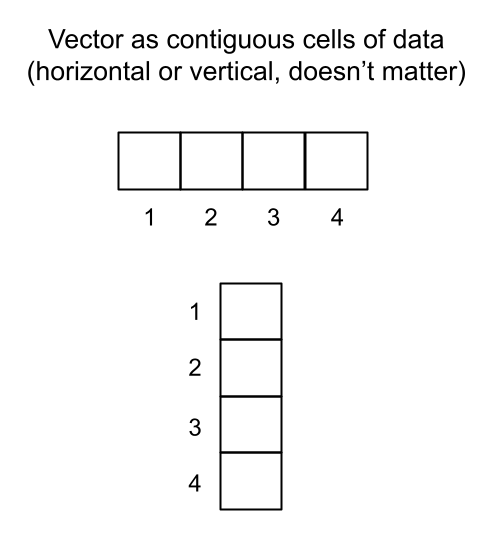
\includegraphics[width=0.4\linewidth]{images/objects/obj-vectors} 

}

\caption{Think of vectors as contiguous cells of data.}\label{fig:unnamed-chunk-16}
\end{figure}

Because this is supposed to be a ``mental representation'' of a vector, you can
think of a vector either horizontally or vertically oriented. It does not
really matter which orientation you prefer to visualize since R has no notion
of a vector's orientation.

Regardless of how you decide to picture a vector in your head, an important
trait of this class of object, and of any other data object in R, is that the
starting position or index is always number 1.

\hypertarget{vectors-are-atomic-objects}{%
\section{Vectors are Atomic Objects}\label{vectors-are-atomic-objects}}

The first thing you should learn about R vectors is that they are considered to
be \textbf{atomic structures}, which is just the fancy name to indicate that all the
elements in a vector are of the \textbf{same type}.

R has four main basic types of atomic vectors:

\begin{itemize}
\item
  \texttt{logical}
\item
  \texttt{integer}
\item
  \texttt{double} or \texttt{real}
\item
  \texttt{character}
\end{itemize}

Here are simple examples of the four common data types of vectors:

\begin{Shaded}
\begin{Highlighting}[]
\CommentTok{\# logical}
\NormalTok{a }\OtherTok{=} \ConstantTok{TRUE}

\CommentTok{\# integer}
\NormalTok{x }\OtherTok{=}\NormalTok{ 1L}

\CommentTok{\# double (real)}
\NormalTok{y }\OtherTok{=} \DecValTok{5}

\CommentTok{\# character}
\NormalTok{b }\OtherTok{=} \StringTok{"yosemite"}
\end{Highlighting}
\end{Shaded}

Logical values, known as boolean values in other languages, are \texttt{TRUE} and
\texttt{FALSE}. These values can be abbreviated by using their first letters \texttt{T} and
\texttt{F}, although I discourage you from doing this because it can make code review
a bit harder. Also, notice that these logical values are specified with upper
case letters. Recall that R is case sensitive, so if you type \texttt{True} or \texttt{False}
R will not recognize them as logical values.

Integer values have an awkward syntax. Notice the appended \texttt{L} when assigning
number 1 to object \texttt{x}. This is not a typo. Rather, this is the syntax used in
R to indicate that a number (with no decimals) is an integer.

If you just simply type a number like \texttt{1} or \texttt{5}, even though cosmetically
they correspond to the mathematical notion of integer numbers, R stores those
numbers as \texttt{double} type. So if you want to declare those numbers as type
\texttt{integer}, you should append an upper case letter \texttt{L} to encode them as \texttt{1L}
and \texttt{5L}.

Character types, referred to as strings in other languages, are specified by
surrounding characters within quotes: either double quotes \texttt{"yosemite"} or
single quotes \texttt{\textquotesingle{}yosemite\textquotesingle{}}. The important thing is to have an opening and a
closing quote of the same kind.

The following diagram summarizes the four common data types of vectors.

\begin{figure}

{\centering 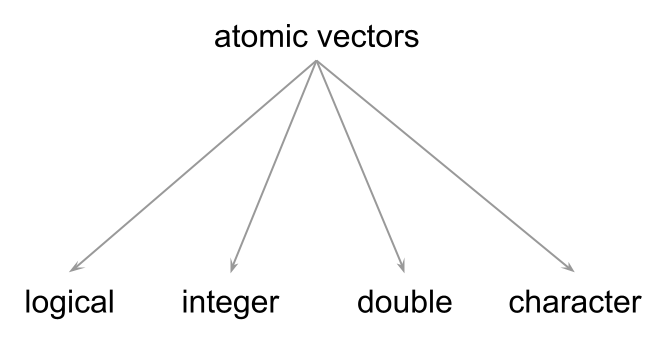
\includegraphics[width=0.55\linewidth]{images/objects/obj-vector-atomic-types} 

}

\caption{Common data types of atomic vectors.}\label{fig:unnamed-chunk-18}
\end{figure}

\hypertarget{complex-and-raw-types}{%
\subsection{Complex and Raw Types}\label{complex-and-raw-types}}

There are two additional types that are less commonly used: \texttt{complex}
(for complex numbers), and \texttt{raw} (raw bytes) which is a binary format used by R.

\begin{figure}

{\centering 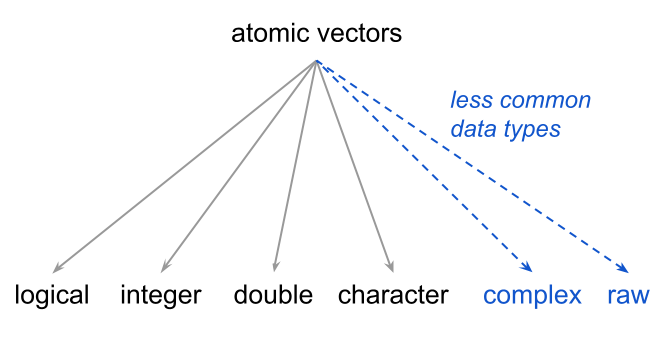
\includegraphics[width=0.6\linewidth]{images/objects/obj-vector-atomic-types2} 

}

\caption{The 4 most common, and 2 less common, data types of atomic vectors.}\label{fig:unnamed-chunk-19}
\end{figure}

I got my first contact with R back in 2001, and I've been using it almost on a
daily basis since 2005. I have never had the need to use \texttt{raw} vectors; R may
be using them in the background but not me (at least not explicitly or
consciously). As for \texttt{complex} numbers, I've seen them every once in a while
when doing certain matrix algebra computations. But again, I haven't
had the need to intentionally work with complex values. I can say the same thing
about most of my colleagues: they rarely use these data types. And I'm willing
to bet that you will rarely use them too. But now you know, if you ever need
to work with \texttt{complex} and/or \texttt{raw} values, they are available in R.

\hypertarget{types-and-modes}{%
\section{Types and Modes}\label{types-and-modes}}

How do you know that a given vector is of a certain data type? For better or
worse, there is a couple of functions that allow you to answer this question:

\begin{itemize}
\item
  \texttt{typeof()}
\item
  \texttt{storage.mode()}
\item
  \texttt{mode()}
\end{itemize}

Although not commonly used within the R community, my recommended function
to determine the data type of a vector is \texttt{typeof()}. The reason for this
recommendation is because \texttt{typeof()} returns the data types previously listed
which are what most other programming languages use:

\begin{Shaded}
\begin{Highlighting}[]
\FunctionTok{typeof}\NormalTok{(deposit)}
\SpecialCharTok{\textgreater{}}\NormalTok{ [}\DecValTok{1}\NormalTok{] }\StringTok{"double"}

\FunctionTok{typeof}\NormalTok{(rate)}
\SpecialCharTok{\textgreater{}}\NormalTok{ [}\DecValTok{1}\NormalTok{] }\StringTok{"double"}
\end{Highlighting}
\end{Shaded}

You should know that among the R community, many useRs don't really talk about
\emph{types}. Instead, because of historical reasons related to the S language---on
which R is based---you will often hear useRs talking about \emph{modes}. To further
complicate matters, there is not just one but two functions related to the
concept of mode: \texttt{storage.mode()} and \texttt{mode()}.

\begin{Shaded}
\begin{Highlighting}[]
\FunctionTok{storage.mode}\NormalTok{(deposit)}
\SpecialCharTok{\textgreater{}}\NormalTok{ [}\DecValTok{1}\NormalTok{] }\StringTok{"double"}

\FunctionTok{mode}\NormalTok{(deposit)}
\SpecialCharTok{\textgreater{}}\NormalTok{ [}\DecValTok{1}\NormalTok{] }\StringTok{"numeric"}
\end{Highlighting}
\end{Shaded}

Both \texttt{storage.mode()} and \texttt{mode()} rely on the output of \texttt{typeof()}, and as
their name indicate, provide information about the storage mode. So what is
the difference between these functions?

For practical purposes, \texttt{storage.mode()} is similar to \texttt{typeof()}, in the
sense that they both return the same output:

\begin{Shaded}
\begin{Highlighting}[]
\FunctionTok{typeof}\NormalTok{(deposit)}
\SpecialCharTok{\textgreater{}}\NormalTok{ [}\DecValTok{1}\NormalTok{] }\StringTok{"double"}

\FunctionTok{storage.mode}\NormalTok{(deposit)}
\SpecialCharTok{\textgreater{}}\NormalTok{ [}\DecValTok{1}\NormalTok{] }\StringTok{"double"}
\end{Highlighting}
\end{Shaded}

In turn, \texttt{mode()} behaves a bit different. \texttt{mode()} groups together types
\texttt{"double"} and \texttt{"integer"} into a single mode called \texttt{"numeric"} because both
data types are numeric values.

\begin{Shaded}
\begin{Highlighting}[]
\FunctionTok{typeof}\NormalTok{(deposit)}
\SpecialCharTok{\textgreater{}}\NormalTok{ [}\DecValTok{1}\NormalTok{] }\StringTok{"double"}

\FunctionTok{mode}\NormalTok{(deposit)}
\SpecialCharTok{\textgreater{}}\NormalTok{ [}\DecValTok{1}\NormalTok{] }\StringTok{"numeric"}
\end{Highlighting}
\end{Shaded}

The following diagram depicts the \texttt{numeric} mode of types \texttt{integer} and
\texttt{double}:

\begin{figure}

{\centering 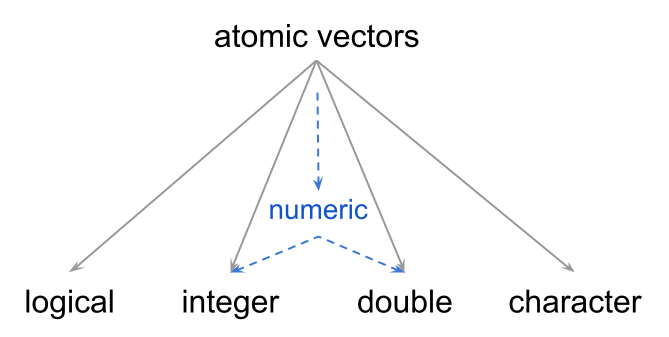
\includegraphics[width=0.55\linewidth]{images/objects/obj-vector-atomic-modes} 

}

\caption{Data types "integer" and "double" correspond to "numeric" mode.}\label{fig:unnamed-chunk-24}
\end{figure}

R also comes with a set of testing functions to determine the type and mode of
a given value:

\begin{itemize}
\item
  \texttt{is.logical()} to test if a value is of type logical
\item
  \texttt{is.integer()} to test if a value is of type integer
\item
  \texttt{is.double()} to test if a value is of type double
\item
  \texttt{is.numeric()} to test if a value is of numeric mode: either integer or double
\item
  \texttt{is.character()} to test if a value is of type character
\end{itemize}

We discuss more details about how R handles data types in chapter
\protect\hyperlink{vectors4}{More About Vectors}.
In the meantime, the following table shows basic examples of each common
data type, and the output of associated functions that give you information
about the type and mode of vectors:

\begin{longtable}[]{@{}cccc@{}}
\toprule()
Example & \texttt{typeof()} & \texttt{storage.mode()} & \texttt{mode()} \\
\midrule()
\endhead
\texttt{TRUE} & \texttt{"logical"} & \texttt{"logical"} & \texttt{"logical"} \\
\texttt{1L} & \texttt{"integer"} & \texttt{"integer"} & \texttt{"numeric"} \\
\texttt{1} & \texttt{"double"} & \texttt{"double"} & \texttt{"numeric"} \\
\texttt{"one"} & \texttt{"character"} & \texttt{"character"} & \texttt{"character"} \\
\bottomrule()
\end{longtable}

\hypertarget{special-values}{%
\section{Special Values}\label{special-values}}

In addition to the four common data types, R also comes with a series of
special values:

\begin{itemize}
\item
  \texttt{NULL} is the null object (it has length zero). The way I like to think of
  this is as ``nothing''; that is, an object that represents ``nothing''.
\item
  \texttt{NA}, which stands for \emph{Not Available}, indicates a missing value. By default,
  typing \texttt{NA} is stored as a logical value. But there are also special types of
  missing values.

  \begin{itemize}
  \tightlist
  \item
    \texttt{NA\_integer\_}
  \item
    \texttt{NA\_real\_}
  \item
    \texttt{NA\_character\_}
  \end{itemize}
\item
  \texttt{NaN} indicates \emph{Not a Number}. An example of this value is the output
  returned by computing the square root of a negative number: \texttt{sqrt(-5)}
\item
  \texttt{Inf} indicates positive infinite, e.g.~\texttt{100/0}
\item
  \texttt{-Inf} indicates negative infinite, e.g.~\texttt{-100/0}
\end{itemize}

R also comes with a set of testing functions to determine if a given value is
of a special kind:

\begin{itemize}
\item
  \texttt{is.null()} to test if a value is \texttt{NULL}
\item
  \texttt{is.na()} to test if a value is \texttt{NA}
\item
  \texttt{is.nan()} to test if a value is \texttt{NaN}
\item
  \texttt{is.infinite()} to test if a value is \texttt{Inf} or \texttt{-Inf}
\end{itemize}

\hypertarget{length-of-vectors}{%
\section{Length of Vectors}\label{length-of-vectors}}

Another important property about vectors is that they have \textbf{length}, which
refers to the number of elements or cells that they contain. If it helps, you
can think of length as the ``size'' of a vector.

The simplest kind of vectors are single values---i.e.~vectors with just one
element. For example, objects such as \texttt{deposit} and \texttt{rate} are one-element
vectors. To find the length of a vector you use the function \texttt{length()}

\begin{Shaded}
\begin{Highlighting}[]
\FunctionTok{length}\NormalTok{(deposit)}
\SpecialCharTok{\textgreater{}}\NormalTok{ [}\DecValTok{1}\NormalTok{] }\DecValTok{1}

\FunctionTok{length}\NormalTok{(amounts)}
\SpecialCharTok{\textgreater{}}\NormalTok{ [}\DecValTok{1}\NormalTok{] }\DecValTok{3}
\end{Highlighting}
\end{Shaded}

By the way, vectors can be of any length, including 0. We talk more about
these special vectors in the next chapter.

\hypertarget{no-scalars-in-r}{%
\subsubsection*{No Scalars in R}\label{no-scalars-in-r}}
\addcontentsline{toc}{subsubsection}{No Scalars in R}

In most other languages, a number like \texttt{5} or a logical \texttt{TRUE} are usually
considered to be ``scalars''. R, however, does not have the concept of ``scalar'',
instead the simplest data structure is that of a one-element vector. This means
that when you type \texttt{5} R handles this data with a vector of length one.

\hypertarget{vector-elements-can-have-names}{%
\section{Vector elements can have names}\label{vector-elements-can-have-names}}

Another feature of vectors is that their elements can have names. For example,
we have the \texttt{amounts} vector that contains the savings amounts at the end of
years 1, 2, and 3:

\begin{Shaded}
\begin{Highlighting}[]
\NormalTok{amounts}
\SpecialCharTok{\textgreater{}}\NormalTok{ [}\DecValTok{1}\NormalTok{] }\FloatTok{1020.000} \FloatTok{1040.400} \FloatTok{1061.208}
\end{Highlighting}
\end{Shaded}

We can give names to the elements in \texttt{amounts} by using the \texttt{names()} function.
We apply \texttt{names()} to \texttt{amounts} and we assign a vector of names like so:

\begin{Shaded}
\begin{Highlighting}[]
\FunctionTok{names}\NormalTok{(amounts) }\OtherTok{=} \FunctionTok{c}\NormalTok{(}\StringTok{"year1"}\NormalTok{, }\StringTok{"year2"}\NormalTok{, }\StringTok{"year3"}\NormalTok{)}
\NormalTok{amounts}
\SpecialCharTok{\textgreater{}}\NormalTok{    year1    year2    year3 }
\SpecialCharTok{\textgreater{}} \FloatTok{1020.000} \FloatTok{1040.400} \FloatTok{1061.208}
\end{Highlighting}
\end{Shaded}

\begin{center}\rule{0.5\linewidth}{0.5pt}\end{center}

\hypertarget{exercises-1}{%
\section{Exercises}\label{exercises-1}}

Consider the following three types of financial products:

\begin{enumerate}
\def\labelenumi{\alph{enumi})}
\item
  joint \textbf{savings account} that pays 2\% annual return, during 2 years,
\item
  joint \textbf{money market account} that pays 3\% annual return, during 3 years
\item
  individual \textbf{certificate of deposit} that pays 4\% annual return, during 4 years
\end{enumerate}

Questions below.

\textbf{1)} Use the \texttt{c()} function to create a character vector \texttt{accounts} such
that when printed it displays the values shown below:

\begin{verbatim}
> [1] "savings"      "money market" "certificate"
\end{verbatim}

\textbf{2)} Use the \texttt{c()} function to create a vector \texttt{joint} of \textbf{logical} values
such that when printed it displays the values shown below:

\begin{verbatim}
> [1]  TRUE  TRUE FALSE
\end{verbatim}

\textbf{3)} Use the \texttt{c()} function to create a vector \texttt{rates} such that when
printed it displays the values shown below:

\begin{verbatim}
> [1] 0.02 0.03 0.04
\end{verbatim}

\textbf{4)} Use the function \texttt{names()} to give names to the elements of your vector \texttt{rates}. When printing \texttt{rates} you should get following output:

\begin{verbatim}
> savings  market  certif 
>    0.02    0.03    0.04
\end{verbatim}

\textbf{5)} Use the \texttt{c()} function to create a vector \texttt{years} of \textbf{integer}
values such that when printed it displays the values shown below. Recall
that integer values are of the form \texttt{1L}.

\begin{verbatim}
> [1] 2 3 4
\end{verbatim}

\textbf{6)} Use the \texttt{typeof()} function to inspect the data type of \texttt{accounts},
\texttt{joint}, \texttt{rates}, and \texttt{years}. Confirm that their output is \texttt{"character"},
\texttt{"logical"}, \texttt{"double"} and \texttt{"integer"}, respectively.

\textbf{7)} Use the \texttt{length()} function to inspect the length of \texttt{accounts},
\texttt{joint}, \texttt{rates}, and \texttt{years}.

\textbf{8)} Explain, in your own words, why vectors are said to be \textbf{atomic} objects.

\textbf{9)} Explain, in your own words, the difference between the output of
functions \texttt{typeof()} and \texttt{mode()}---when applied to vectors.

\hypertarget{vectors3}{%
\chapter{Creating Vectors}\label{vectors3}}

In the preceding chapter you started learning about the basic properties of
vectors. We focused on the common flavors of vectors (e.g.~logical, integer,
double, and character), reviewed special values (e.g.~\texttt{NULL}, \texttt{NA}), talked
about the length or size of a vector, and we also mentioned that elements in a
vector can have names.

Likewise, you have seen two basic ways to create simple vectors:

\begin{itemize}
\item
  creation of one-element vectors, e.g.~\texttt{money\ =\ 100}, \texttt{rate\ =\ 0.02},
  \texttt{account\ =\ "savings"}
\item
  creation of more than one-element, yet small, vectors with the combine
  function \texttt{c()}, e.g.~\texttt{years\ =\ c(1L,\ 2L,\ 3L)}.
\end{itemize}

In this chapter I discuss two broad topics: 1) a review of various functions
and ways to \textbf{create vectors}, and 2) a description of the \textbf{coercion} notion.
Why should you learn about various forms of vector creation in R? Because as I
said, R is---to a large extent---a vector-based language, and you have to be
ready to create multiple kinds of vectors, and to take advantage of some of the
mechanisms that R provides for doing this. As for the topic of coercion, you
also need to understand the behavior of R when working with vectors of different
data types.

\hypertarget{creating-vectors-with-c}{%
\section{\texorpdfstring{Creating vectors with \texttt{c()}}{Creating vectors with c()}}\label{creating-vectors-with-c}}

We've seen how to create simple vectors containing just one element (i.e.~
length-1 vectors)

\begin{Shaded}
\begin{Highlighting}[]
\CommentTok{\# inputs}
\NormalTok{deposit }\OtherTok{=} \DecValTok{1000}
\NormalTok{rate }\OtherTok{=} \FloatTok{0.02}

\CommentTok{\# amounts at the end of years 1, 2, and 3}
\NormalTok{amount1 }\OtherTok{=}\NormalTok{ deposit }\SpecialCharTok{*}\NormalTok{ (}\DecValTok{1} \SpecialCharTok{+}\NormalTok{ rate)}
\NormalTok{amount2 }\OtherTok{=}\NormalTok{ amount1 }\SpecialCharTok{*}\NormalTok{ (}\DecValTok{1} \SpecialCharTok{+}\NormalTok{ rate)}
\NormalTok{amount3 }\OtherTok{=}\NormalTok{ amount2 }\SpecialCharTok{*}\NormalTok{ (}\DecValTok{1} \SpecialCharTok{+}\NormalTok{ rate)}
\end{Highlighting}
\end{Shaded}

We've also seen the basic use of the \textbf{combine} function \texttt{c()} to create a
vector containing several elements:

\begin{Shaded}
\begin{Highlighting}[]
\CommentTok{\# combine amounts in a single vector}
\NormalTok{amounts }\OtherTok{=} \FunctionTok{c}\NormalTok{(amount1, amount2, amount3)}
\NormalTok{amounts}
\SpecialCharTok{\textgreater{}}\NormalTok{ [}\DecValTok{1}\NormalTok{] }\FloatTok{1020.000} \FloatTok{1040.400} \FloatTok{1061.208}
\end{Highlighting}
\end{Shaded}

The \texttt{c()} function is one of the primary functions to create vectors of length
greater than one. Here's another example for how to create a vector \texttt{flavors}
with some ice-cream flavors:

\begin{Shaded}
\begin{Highlighting}[]
\NormalTok{flavors }\OtherTok{\textless{}{-}} \FunctionTok{c}\NormalTok{(}\StringTok{"lemon"}\NormalTok{, }\StringTok{"vanilla"}\NormalTok{, }\StringTok{"chocolate"}\NormalTok{)}

\NormalTok{flavors}
\SpecialCharTok{\textgreater{}}\NormalTok{ [}\DecValTok{1}\NormalTok{] }\StringTok{"lemon"}     \StringTok{"vanilla"}   \StringTok{"chocolate"}
\end{Highlighting}
\end{Shaded}

Basically, you call \texttt{c()} and you type in the values, separating them by
commas.

If your vector has only one element, you don't need to call the \texttt{c()} function.

\begin{Shaded}
\begin{Highlighting}[]
\CommentTok{\# no need to use c() to create a one{-}element vector}
\NormalTok{lemon }\OtherTok{=} \FunctionTok{c}\NormalTok{(}\StringTok{"lemon"}\NormalTok{)}

\CommentTok{\# instead just do this}
\NormalTok{lemon }\OtherTok{=} \StringTok{"lemon"}
\end{Highlighting}
\end{Shaded}

One more thing that you can do when using \texttt{c()} is to give names to the
elements of the created vector. This is done by joining pairs of
values of the form: \texttt{\textquotesingle{}name\textquotesingle{}\ =\ value}, where \texttt{\textquotesingle{}name\textquotesingle{}} is the name given to the
\texttt{value} of an element. For instance, you can create the vector
\texttt{amounts} and give names to each element like this:

\begin{Shaded}
\begin{Highlighting}[]
\CommentTok{\# give names to elements when using c()}
\CommentTok{\# (names specified with quotes)}
\NormalTok{amounts }\OtherTok{=} \FunctionTok{c}\NormalTok{(}
  \StringTok{"year1"} \OtherTok{=}\NormalTok{ amount1, }
  \StringTok{"year2"} \OtherTok{=}\NormalTok{ amount2, }
  \StringTok{"year3"} \OtherTok{=}\NormalTok{ amount3)}

\NormalTok{amounts}
\SpecialCharTok{\textgreater{}}\NormalTok{    year1    year2    year3 }
\SpecialCharTok{\textgreater{}} \FloatTok{1020.000} \FloatTok{1040.400} \FloatTok{1061.208}
\end{Highlighting}
\end{Shaded}

As you can tell, the names of each element are specified as \texttt{character} values:
\texttt{"year1"}, \texttt{"year2"}, and \texttt{"year3"}. Interestingly, you can also
specify names without quoting them:

\begin{Shaded}
\begin{Highlighting}[]
\CommentTok{\# give names to elements when using c()}
\CommentTok{\# (names unquoted)}
\NormalTok{amounts2 }\OtherTok{=} \FunctionTok{c}\NormalTok{(}
  \AttributeTok{year1 =}\NormalTok{ amount1, }
  \AttributeTok{year2 =}\NormalTok{ amount2, }
  \AttributeTok{year3 =}\NormalTok{ amount3)}

\NormalTok{amounts2}
\SpecialCharTok{\textgreater{}}\NormalTok{    year1    year2    year3 }
\SpecialCharTok{\textgreater{}} \FloatTok{1020.000} \FloatTok{1040.400} \FloatTok{1061.208}
\end{Highlighting}
\end{Shaded}

This way of giving names to the elements of a vector can feel a bit surprising,
especially to users that have previous programming experience but are new to
the R syntax. Personally, I don't really care about having 2 different---and
apparently confusing---ways to give names to elements when using functions like
\texttt{c()}. Having said that, I can perfectly understand the initial shock and
confusion that this may cause to non-experienced useRs.

To be consistent with most other languages, and also to play defensively,
I tend to recommend quoting the values that are supposed to be the
names of the elements in a vector. Again, this is my personal biased
suggestion, and it is not a rule by any means.

\hypertarget{default-vectors}{%
\section{Default Vectors}\label{default-vectors}}

R comes with a set of functions to initialize vectors of a specific data type.
The generic function is \texttt{vector()} but there are also type-specific versions:

\begin{itemize}
\item
  \texttt{vector()}
\item
  \texttt{logical()}
\item
  \texttt{integer()}
\item
  \texttt{double()} and \texttt{numeric()}
\item
  \texttt{character()}
\end{itemize}

The function \texttt{vector()}, as the name indicates, lets you create a vector of
a given \texttt{mode} and of a certain \texttt{length}. By default, \texttt{vector()} creates a
\texttt{"logical"} vector of \texttt{length\ =\ 0}.

\begin{Shaded}
\begin{Highlighting}[]
\NormalTok{log }\OtherTok{=} \FunctionTok{vector}\NormalTok{()}
\NormalTok{log}
\SpecialCharTok{\textgreater{}} \FunctionTok{logical}\NormalTok{(}\DecValTok{0}\NormalTok{)}

\FunctionTok{length}\NormalTok{(log)}
\SpecialCharTok{\textgreater{}}\NormalTok{ [}\DecValTok{1}\NormalTok{] }\DecValTok{0}
\end{Highlighting}
\end{Shaded}

Notice what happens when you print \texttt{log}, the output displayed is: \texttt{logical(0)}.
This is the notation that R uses to indicate that a vector is of length zero.
The previous call is equivalent to:

\begin{Shaded}
\begin{Highlighting}[]
\FunctionTok{vector}\NormalTok{(}\AttributeTok{mode =} \StringTok{"logical"}\NormalTok{, }\AttributeTok{length =} \DecValTok{0}\NormalTok{)}
\end{Highlighting}
\end{Shaded}

A common question that some useRs have when they encounter things like
\texttt{logical(0)} is ``when do you use zero-length vectors''? The quick answer is:
you can use zero-length vectors to initialize a vector that will later be
populated with more elements. This typically happens when you know that a
vector of certain type is needed to store several values, but you don't know
in advance how many elements will be computed.

All the other functions, e.g.~\texttt{logical()}, \texttt{integer()}, etc, take just one
argument \texttt{length} to indicate the number of elements of the output vector.
Keep in mind that the value(s) of the initialized vector cannot be changed:

\begin{Shaded}
\begin{Highlighting}[]
\FunctionTok{logical}\NormalTok{(}\AttributeTok{length =} \DecValTok{1}\NormalTok{)}
\SpecialCharTok{\textgreater{}}\NormalTok{ [}\DecValTok{1}\NormalTok{] }\ConstantTok{FALSE}

\FunctionTok{integer}\NormalTok{(}\AttributeTok{length =} \DecValTok{2}\NormalTok{)}
\SpecialCharTok{\textgreater{}}\NormalTok{ [}\DecValTok{1}\NormalTok{] }\DecValTok{0} \DecValTok{0}

\FunctionTok{double}\NormalTok{(}\AttributeTok{length =} \DecValTok{3}\NormalTok{)}
\SpecialCharTok{\textgreater{}}\NormalTok{ [}\DecValTok{1}\NormalTok{] }\DecValTok{0} \DecValTok{0} \DecValTok{0}

\FunctionTok{character}\NormalTok{(}\AttributeTok{length =} \DecValTok{4}\NormalTok{)}
\SpecialCharTok{\textgreater{}}\NormalTok{ [}\DecValTok{1}\NormalTok{] }\StringTok{""} \StringTok{""} \StringTok{""} \StringTok{""}
\end{Highlighting}
\end{Shaded}

\hypertarget{numeric-sequences}{%
\section{Numeric Sequences}\label{numeric-sequences}}

A common situation when creating vectors involves creating numeric sequences.
If the numeric sequence is short and simple, it could be created with the
combine function \texttt{c()}, for example:

\begin{Shaded}
\begin{Highlighting}[]
\NormalTok{s1 }\OtherTok{=} \FunctionTok{c}\NormalTok{(}\DecValTok{1}\NormalTok{, }\DecValTok{2}\NormalTok{, }\DecValTok{3}\NormalTok{, }\DecValTok{4}\NormalTok{)}
\NormalTok{s1}
\SpecialCharTok{\textgreater{}}\NormalTok{ [}\DecValTok{1}\NormalTok{] }\DecValTok{1} \DecValTok{2} \DecValTok{3} \DecValTok{4}
\end{Highlighting}
\end{Shaded}

Often, you will have to create less simpler and/or longer sequences. For these
purposes there are two useful functions:

\begin{itemize}
\item
  the colon operator \texttt{":"}
\item
  the sequence function \texttt{seq()} and its siblings \texttt{seq.int()}, \texttt{seq\_along()}
  and \texttt{seq.len()}
\end{itemize}

\hypertarget{sequences-with}{%
\subsection{\texorpdfstring{Sequences with \texttt{:}}{Sequences with :}}\label{sequences-with}}

The colon operator \texttt{:} lets you create numeric sequences by indicating the
starting and ending values. For instance, if you want to generate an integer
sequence starting at 1 and ending at 10, you use this command:

\begin{Shaded}
\begin{Highlighting}[]
\NormalTok{ints }\OtherTok{=} \DecValTok{1}\SpecialCharTok{:}\DecValTok{10}
\NormalTok{ints}
\SpecialCharTok{\textgreater{}}\NormalTok{  [}\DecValTok{1}\NormalTok{]  }\DecValTok{1}  \DecValTok{2}  \DecValTok{3}  \DecValTok{4}  \DecValTok{5}  \DecValTok{6}  \DecValTok{7}  \DecValTok{8}  \DecValTok{9} \DecValTok{10}
\end{Highlighting}
\end{Shaded}

Notice that the colon operator, when used with whole numbers, will produce
an integer sequence

\begin{Shaded}
\begin{Highlighting}[]
\FunctionTok{typeof}\NormalTok{(ints)}
\SpecialCharTok{\textgreater{}}\NormalTok{ [}\DecValTok{1}\NormalTok{] }\StringTok{"integer"}
\end{Highlighting}
\end{Shaded}

However, when the starting value is not a whole number, then the generated
sequence will be of type \texttt{double}, with one-unit steps. For example:

\begin{Shaded}
\begin{Highlighting}[]
\NormalTok{dbls }\OtherTok{=} \FloatTok{1.5}\SpecialCharTok{:}\FloatTok{5.5}
\NormalTok{dbls}
\SpecialCharTok{\textgreater{}}\NormalTok{ [}\DecValTok{1}\NormalTok{] }\FloatTok{1.5} \FloatTok{2.5} \FloatTok{3.5} \FloatTok{4.5} \FloatTok{5.5}

\FunctionTok{typeof}\NormalTok{(dbls)}
\SpecialCharTok{\textgreater{}}\NormalTok{ [}\DecValTok{1}\NormalTok{] }\StringTok{"double"}
\end{Highlighting}
\end{Shaded}

Run the following commands to see how R generates different sequences:

\begin{Shaded}
\begin{Highlighting}[]
\FloatTok{1.5}\SpecialCharTok{:}\DecValTok{5}
\FloatTok{1.5}\SpecialCharTok{:}\FloatTok{5.1}
\FloatTok{1.5}\SpecialCharTok{:}\FloatTok{5.5}
\FloatTok{1.5}\SpecialCharTok{:}\FloatTok{5.9}
\end{Highlighting}
\end{Shaded}

You can also create a \textbf{descending} sequence by starting with a value on the
left-hand side of \texttt{:} that is greater than the value on the right-hand side:

\begin{Shaded}
\begin{Highlighting}[]
\CommentTok{\# descending (reversed) sequence}
\DecValTok{10}\SpecialCharTok{:}\DecValTok{1}
\SpecialCharTok{\textgreater{}}\NormalTok{  [}\DecValTok{1}\NormalTok{] }\DecValTok{10}  \DecValTok{9}  \DecValTok{8}  \DecValTok{7}  \DecValTok{6}  \DecValTok{5}  \DecValTok{4}  \DecValTok{3}  \DecValTok{2}  \DecValTok{1}
\end{Highlighting}
\end{Shaded}

\begin{Shaded}
\begin{Highlighting}[]
\CommentTok{\# this also applies to negative numbers}
\SpecialCharTok{{-}}\DecValTok{10}\SpecialCharTok{:{-}}\DecValTok{1}
\SpecialCharTok{\textgreater{}}\NormalTok{  [}\DecValTok{1}\NormalTok{] }\SpecialCharTok{{-}}\DecValTok{10}  \SpecialCharTok{{-}}\DecValTok{9}  \SpecialCharTok{{-}}\DecValTok{8}  \SpecialCharTok{{-}}\DecValTok{7}  \SpecialCharTok{{-}}\DecValTok{6}  \SpecialCharTok{{-}}\DecValTok{5}  \SpecialCharTok{{-}}\DecValTok{4}  \SpecialCharTok{{-}}\DecValTok{3}  \SpecialCharTok{{-}}\DecValTok{2}  \SpecialCharTok{{-}}\DecValTok{1}
\end{Highlighting}
\end{Shaded}

\hypertarget{sequences-with-seq}{%
\subsection{\texorpdfstring{Sequences with \texttt{seq()}}{Sequences with seq()}}\label{sequences-with-seq}}

The colon operator \texttt{:} can be very useful but it has its limitations. Its main
downside is that the generated sequences are of one-unit steps. But what if
you want a sequence with steps different from one-unit? For instance, what if
you are interested in something like: \texttt{2,\ 4,\ 6,\ 8,\ ...}?

In addition to the colon operator, R also provides the more generic \texttt{seq()}
function for creating numeric sequences. This function comes with a couple of
parameters that let you generate sequences in various forms.

The simplest usage of \texttt{seq()} involves passing values for the arguments \texttt{from}
(the starting value) and \texttt{to} (the ending value):

\begin{Shaded}
\begin{Highlighting}[]
\CommentTok{\# equivalent to 1:10}
\FunctionTok{seq}\NormalTok{(}\AttributeTok{from =} \DecValTok{1}\NormalTok{, }\AttributeTok{to =} \DecValTok{10}\NormalTok{)}
\SpecialCharTok{\textgreater{}}\NormalTok{  [}\DecValTok{1}\NormalTok{]  }\DecValTok{1}  \DecValTok{2}  \DecValTok{3}  \DecValTok{4}  \DecValTok{5}  \DecValTok{6}  \DecValTok{7}  \DecValTok{8}  \DecValTok{9} \DecValTok{10}
\end{Highlighting}
\end{Shaded}

As you can tell, the sequence is created with one-unit steps. But this can
be changed with the \texttt{by} argument. Say you want steps of two-units, then
specify \texttt{by\ =\ 2}:

\begin{Shaded}
\begin{Highlighting}[]
\FunctionTok{seq}\NormalTok{(}\AttributeTok{from =} \DecValTok{1}\NormalTok{, }\AttributeTok{to =} \DecValTok{10}\NormalTok{, }\AttributeTok{by =} \DecValTok{2}\NormalTok{)}
\SpecialCharTok{\textgreater{}}\NormalTok{ [}\DecValTok{1}\NormalTok{] }\DecValTok{1} \DecValTok{3} \DecValTok{5} \DecValTok{7} \DecValTok{9}
\end{Highlighting}
\end{Shaded}

Now, what if you want a decreasing sequence, for example 10, 9, \ldots, 1?
You can also use \texttt{seq()} to achieve this goal. The starting value \texttt{from} is 10,
the ending value \texttt{to} is 1, and the step size \texttt{by} has to be \texttt{-1}

\begin{Shaded}
\begin{Highlighting}[]
\FunctionTok{seq}\NormalTok{(}\AttributeTok{from =} \DecValTok{10}\NormalTok{, }\AttributeTok{to =} \DecValTok{1}\NormalTok{, }\AttributeTok{by =} \SpecialCharTok{{-}}\DecValTok{1}\NormalTok{)}
\SpecialCharTok{\textgreater{}}\NormalTok{  [}\DecValTok{1}\NormalTok{] }\DecValTok{10}  \DecValTok{9}  \DecValTok{8}  \DecValTok{7}  \DecValTok{6}  \DecValTok{5}  \DecValTok{4}  \DecValTok{3}  \DecValTok{2}  \DecValTok{1}
\end{Highlighting}
\end{Shaded}

Sometimes you may be interested in creating a sequence of a specific length.
When this is the case, you need to use the \texttt{length.out} argument. For example,
say we want to start with 2, getting the sequence of the first six even numbers.
One way to obtain this sequence is with \texttt{from\ =\ 2}, steps of size \texttt{by\ =\ 2},
and a length of \texttt{length.out\ =\ 6}

\begin{Shaded}
\begin{Highlighting}[]
\FunctionTok{seq}\NormalTok{(}\AttributeTok{from =} \DecValTok{2}\NormalTok{, }\AttributeTok{length.out =} \DecValTok{6}\NormalTok{, }\AttributeTok{by =} \DecValTok{2}\NormalTok{)}
\SpecialCharTok{\textgreater{}}\NormalTok{ [}\DecValTok{1}\NormalTok{]  }\DecValTok{2}  \DecValTok{4}  \DecValTok{6}  \DecValTok{8} \DecValTok{10} \DecValTok{12}
\end{Highlighting}
\end{Shaded}

\hypertarget{sequences-with-seq_len-and-seq_along}{%
\subsection{\texorpdfstring{Sequences with \texttt{seq\_len()} and \texttt{seq\_along()}}{Sequences with seq\_len() and seq\_along()}}\label{sequences-with-seq_len-and-seq_along}}

\texttt{seq()} comes with sibling functions such as \texttt{seq.int()}, \texttt{seq\_len()} and
\texttt{seq\_along()}. These are more specialized functions than the generic \texttt{seq()},
and they can be more efficient to generate certain sequences.

The function \texttt{seq.int()} is designed to generate integer sequences. The
difference against \texttt{seq()} is that \texttt{seq.int()} is more efficient:

\begin{Shaded}
\begin{Highlighting}[]
\CommentTok{\# equivalent to seq(from = 5, to = 10), but more efficient}
\FunctionTok{seq.int}\NormalTok{(}\AttributeTok{from =} \DecValTok{5}\NormalTok{, }\AttributeTok{to =} \DecValTok{10}\NormalTok{)}
\SpecialCharTok{\textgreater{}}\NormalTok{ [}\DecValTok{1}\NormalTok{]  }\DecValTok{5}  \DecValTok{6}  \DecValTok{7}  \DecValTok{8}  \DecValTok{9} \DecValTok{10}
\end{Highlighting}
\end{Shaded}

If you want a sequence of consecutive positive integers starting at 1,
\texttt{seq\_len()} is your friend:

\begin{Shaded}
\begin{Highlighting}[]
\CommentTok{\# equivalent to seq(from = 1, to = 10), but more efficient}
\FunctionTok{seq\_len}\NormalTok{(}\DecValTok{10}\NormalTok{)}
\SpecialCharTok{\textgreater{}}\NormalTok{  [}\DecValTok{1}\NormalTok{]  }\DecValTok{1}  \DecValTok{2}  \DecValTok{3}  \DecValTok{4}  \DecValTok{5}  \DecValTok{6}  \DecValTok{7}  \DecValTok{8}  \DecValTok{9} \DecValTok{10}
\end{Highlighting}
\end{Shaded}

The third type of sequence function is \texttt{seq\_along()}. This function takes
a vector of any length, and it produces a sequence of consecutive positive
integers of the same length as the input vector.

\begin{Shaded}
\begin{Highlighting}[]
\NormalTok{accounts }\OtherTok{=} \FunctionTok{c}\NormalTok{(}\StringTok{"savings"}\NormalTok{, }\StringTok{"checking"}\NormalTok{, }\StringTok{"brokerage"}\NormalTok{, }\StringTok{"retirement"}\NormalTok{)}
\FunctionTok{seq\_along}\NormalTok{(accounts)}
\SpecialCharTok{\textgreater{}}\NormalTok{ [}\DecValTok{1}\NormalTok{] }\DecValTok{1} \DecValTok{2} \DecValTok{3} \DecValTok{4}
\end{Highlighting}
\end{Shaded}

If the input vector has length zero, then \texttt{seq\_along()} returns zero

\begin{Shaded}
\begin{Highlighting}[]
\NormalTok{null }\OtherTok{=} \ConstantTok{NULL}  \CommentTok{\# length(null) is zero}
\FunctionTok{seq\_along}\NormalTok{(null)}
\SpecialCharTok{\textgreater{}} \FunctionTok{integer}\NormalTok{(}\DecValTok{0}\NormalTok{)}
\end{Highlighting}
\end{Shaded}

\hypertarget{replicated-vectors}{%
\section{Replicated Vectors}\label{replicated-vectors}}

Some times you need to create vectors containing repeated elements. To do this
you can use the function \texttt{rep()}. This function takes a vector as the main
input, and then it optionally takes various arguments: \texttt{times}, \texttt{length.out},
and \texttt{each} that let you control the way in which the elements of the input
vector should be repeated.

\begin{Shaded}
\begin{Highlighting}[]
\FunctionTok{rep}\NormalTok{(}\DecValTok{1}\NormalTok{, }\AttributeTok{times =} \DecValTok{5}\NormalTok{)        }\CommentTok{\# repeat 1 five times}
\SpecialCharTok{\textgreater{}}\NormalTok{ [}\DecValTok{1}\NormalTok{] }\DecValTok{1} \DecValTok{1} \DecValTok{1} \DecValTok{1} \DecValTok{1}

\FunctionTok{rep}\NormalTok{(}\FunctionTok{c}\NormalTok{(}\DecValTok{1}\NormalTok{, }\DecValTok{2}\NormalTok{), }\AttributeTok{times =} \DecValTok{3}\NormalTok{)  }\CommentTok{\# repeat 1 2 three times}
\SpecialCharTok{\textgreater{}}\NormalTok{ [}\DecValTok{1}\NormalTok{] }\DecValTok{1} \DecValTok{2} \DecValTok{1} \DecValTok{2} \DecValTok{1} \DecValTok{2}

\FunctionTok{rep}\NormalTok{(}\FunctionTok{c}\NormalTok{(}\DecValTok{1}\NormalTok{, }\DecValTok{2}\NormalTok{), }\AttributeTok{each =} \DecValTok{2}\NormalTok{)   }\CommentTok{\# each element repeated twice}
\SpecialCharTok{\textgreater{}}\NormalTok{ [}\DecValTok{1}\NormalTok{] }\DecValTok{1} \DecValTok{1} \DecValTok{2} \DecValTok{2}

\FunctionTok{rep}\NormalTok{(}\FunctionTok{c}\NormalTok{(}\DecValTok{1}\NormalTok{, }\DecValTok{2}\NormalTok{), }\AttributeTok{length.out =} \DecValTok{5}\NormalTok{)  }\CommentTok{\# repeat until length of 5}
\SpecialCharTok{\textgreater{}}\NormalTok{ [}\DecValTok{1}\NormalTok{] }\DecValTok{1} \DecValTok{2} \DecValTok{1} \DecValTok{2} \DecValTok{1}
\end{Highlighting}
\end{Shaded}

Here are two less simple examples:

\begin{Shaded}
\begin{Highlighting}[]
\FunctionTok{rep}\NormalTok{(}\FunctionTok{c}\NormalTok{(}\DecValTok{3}\NormalTok{, }\DecValTok{2}\NormalTok{, }\DecValTok{1}\NormalTok{), }\AttributeTok{times =} \DecValTok{3}\SpecialCharTok{:}\DecValTok{1}\NormalTok{)}
\SpecialCharTok{\textgreater{}}\NormalTok{ [}\DecValTok{1}\NormalTok{] }\DecValTok{3} \DecValTok{3} \DecValTok{3} \DecValTok{2} \DecValTok{2} \DecValTok{1}

\FunctionTok{rep}\NormalTok{(}\FunctionTok{c}\NormalTok{(}\DecValTok{3}\NormalTok{, }\DecValTok{2}\NormalTok{, }\DecValTok{1}\NormalTok{), }\AttributeTok{times =} \DecValTok{3}\NormalTok{, }\AttributeTok{each =} \DecValTok{2}\NormalTok{)}
\SpecialCharTok{\textgreater{}}\NormalTok{  [}\DecValTok{1}\NormalTok{] }\DecValTok{3} \DecValTok{3} \DecValTok{2} \DecValTok{2} \DecValTok{1} \DecValTok{1} \DecValTok{3} \DecValTok{3} \DecValTok{2} \DecValTok{2} \DecValTok{1} \DecValTok{1} \DecValTok{3} \DecValTok{3} \DecValTok{2} \DecValTok{2} \DecValTok{1} \DecValTok{1}
\end{Highlighting}
\end{Shaded}

\hypertarget{coercion}{%
\section{Coercion}\label{coercion}}

One of the basic properties of vectors that you learned in the preceding chapter
is that vectors are \emph{atomic} objects. This is just the fancy way to say that all
the elements of a vector have to be of the same data type. If I show you the
following vectors, and ask you about their data types, you should have no
problem answering this question:

\begin{Shaded}
\begin{Highlighting}[]
\NormalTok{one }\OtherTok{=} \FunctionTok{c}\NormalTok{(}\ConstantTok{TRUE}\NormalTok{, }\ConstantTok{FALSE}\NormalTok{)}
\NormalTok{two }\OtherTok{=} \DecValTok{2}\SpecialCharTok{:}\DecValTok{4}
\NormalTok{three }\OtherTok{=} \FunctionTok{c}\NormalTok{(}\DecValTok{11}\NormalTok{, }\DecValTok{22}\NormalTok{, }\DecValTok{33}\NormalTok{)}
\NormalTok{four }\OtherTok{=} \FunctionTok{c}\NormalTok{(}\StringTok{"one"}\NormalTok{, }\StringTok{"two"}\NormalTok{, }\StringTok{"three"}\NormalTok{)}
\end{Highlighting}
\end{Shaded}

If you have doubts about the data type of any of the above vectors, recall
that you can use \texttt{typeof()} to get the answer.

But what if I create vectors by mixing elements of different data types? For
example:

\begin{Shaded}
\begin{Highlighting}[]
\NormalTok{uno }\OtherTok{=} \FunctionTok{c}\NormalTok{(}\ConstantTok{FALSE}\NormalTok{, 1L)    }\CommentTok{\# logical \& integer}
\NormalTok{dos }\OtherTok{=} \FunctionTok{c}\NormalTok{(1L, 2L, }\DecValTok{3}\NormalTok{)    }\CommentTok{\# integer \& double}
\NormalTok{tres }\OtherTok{=} \FunctionTok{c}\NormalTok{(}\DecValTok{1}\NormalTok{, }\DecValTok{2}\NormalTok{, }\StringTok{"3"}\NormalTok{)   }\CommentTok{\# double \& character}
\end{Highlighting}
\end{Shaded}

Enter \textbf{coercion} principles!

Coercion is another fundamental concept that you should learn about vectors.
This has to do with the mechanisms that R uses to make sure that all the
elements in a vector are of the same data type.

There are two coercion mechanisms or approaches:

\begin{itemize}
\item
  implicit coercion rules
\item
  explicit coercion functions
\end{itemize}

\hypertarget{implicit-coercion-rules}{%
\subsection{Implicit Coercion Rules}\label{implicit-coercion-rules}}

\textbf{Implicit coercion} is what R does when we try to combine values of different
types into a single vector. Here's an example:

\begin{Shaded}
\begin{Highlighting}[]
\NormalTok{mixed }\OtherTok{\textless{}{-}} \FunctionTok{c}\NormalTok{(}\ConstantTok{TRUE}\NormalTok{, 1L, }\FloatTok{2.0}\NormalTok{, }\StringTok{"three"}\NormalTok{)}
\NormalTok{mixed}
\SpecialCharTok{\textgreater{}}\NormalTok{ [}\DecValTok{1}\NormalTok{] }\StringTok{"TRUE"}  \StringTok{"1"}     \StringTok{"2"}     \StringTok{"three"}
\end{Highlighting}
\end{Shaded}

In this command we are mixing different data types: a logical \texttt{TRUE}, an integer
\texttt{1L}, a double \texttt{2.0}, and a character \texttt{"three"}. Now, even though the input
values are of different data flavors, R has decided to convert everything into
type \texttt{"character"}. Technically speaking, R has \textbf{implicitly coerced} the
values as characters, without asking for our permission and without even
letting us know that it did so.

If you are not familiar with implicit coercion rules, you may get an initial
impression that R is acting weirdly, in a nonsensical form. The more you get
familiar with R, you will notice some interesting coercion patterns. But you
don't need to struggle figuring out what R will do. You just have to remember
the following hierarchy:

\[
\mathsf{character > double > integer > logical}
\]

Here's how R works in terms of coercion:

\begin{itemize}
\item
  characters have priority over other data types: as long as one element is
  a character, all other elements are coerced into characters
\item
  if a vector has numbers (double and integer) and logicals, double will
  dominate
\item
  finally, when mixing integers and logicals, integers will dominate
\end{itemize}

Also, when certain operations are applied to certain data types, R may apply
its coercion rules. An example of this behavior is when you have a logical
vector on which you apply arithmetic operations:

\begin{Shaded}
\begin{Highlighting}[]
\CommentTok{\# logical vector}
\NormalTok{logs }\OtherTok{=} \FunctionTok{c}\NormalTok{(}\ConstantTok{TRUE}\NormalTok{, }\ConstantTok{FALSE}\NormalTok{, }\ConstantTok{TRUE}\NormalTok{)}

\CommentTok{\# addition (creates integers)}
\NormalTok{logs2 }\OtherTok{=}\NormalTok{ logs }\SpecialCharTok{+}\NormalTok{ logs}
\FunctionTok{typeof}\NormalTok{(logs2)}
\SpecialCharTok{\textgreater{}}\NormalTok{ [}\DecValTok{1}\NormalTok{] }\StringTok{"integer"}

\CommentTok{\# multiplication (creates doubles)}
\NormalTok{logs3 }\OtherTok{=}\NormalTok{ logs }\SpecialCharTok{*} \DecValTok{3}
\FunctionTok{typeof}\NormalTok{(logs3)}
\SpecialCharTok{\textgreater{}}\NormalTok{ [}\DecValTok{1}\NormalTok{] }\StringTok{"double"}
\end{Highlighting}
\end{Shaded}

\hypertarget{explicit-coercion-functions}{%
\subsection{Explicit Coercion Functions}\label{explicit-coercion-functions}}

The other type of coercion mechanism, known as \textbf{explicit coercion}, is done
when you explicitly tell R to convert a certain type of vector into a different
data type by using explicit coercion functions such as:

\begin{itemize}
\tightlist
\item
  \texttt{as.integer()}
\item
  \texttt{as.double()}
\item
  \texttt{as.character()}
\item
  \texttt{as.logical()}
\end{itemize}

Depending on the type of input vector, and the coercion function, you may
achieve what you want, or R may fail to convert things accordingly.

We can take \texttt{deposit}, which is of type double, and convert it into an integer
with no issues:

\begin{Shaded}
\begin{Highlighting}[]
\NormalTok{int\_deposit }\OtherTok{=} \FunctionTok{as.integer}\NormalTok{(deposit)}
\NormalTok{int\_deposit}
\SpecialCharTok{\textgreater{}}\NormalTok{ [}\DecValTok{1}\NormalTok{] }\DecValTok{1000}
\end{Highlighting}
\end{Shaded}

Interestingly, the way an \texttt{integer} number is displayed is exactly the same
as its \texttt{double} version. To confirm that \texttt{int\_deposit} is indeed of type
\texttt{integer} you can use the \texttt{is.integer()} function

\begin{Shaded}
\begin{Highlighting}[]
\FunctionTok{is.integer}\NormalTok{(deposit)}
\SpecialCharTok{\textgreater{}}\NormalTok{ [}\DecValTok{1}\NormalTok{] }\ConstantTok{FALSE}
\FunctionTok{is.integer}\NormalTok{(int\_deposit)}
\SpecialCharTok{\textgreater{}}\NormalTok{ [}\DecValTok{1}\NormalTok{] }\ConstantTok{TRUE}
\end{Highlighting}
\end{Shaded}

What about trying to convert a character string such as \texttt{"string"} into an
integer? You can try to apply \texttt{as.integer()} but in this case the attempt is
fruitless:

\begin{Shaded}
\begin{Highlighting}[]
\FunctionTok{as.integer}\NormalTok{(}\StringTok{"string"}\NormalTok{)}
\SpecialCharTok{\textgreater{}}\NormalTok{ Warning}\SpecialCharTok{:}\NormalTok{ NAs introduced by coercion}
\SpecialCharTok{\textgreater{}}\NormalTok{ [}\DecValTok{1}\NormalTok{] }\ConstantTok{NA}
\end{Highlighting}
\end{Shaded}

\begin{center}\rule{0.5\linewidth}{0.5pt}\end{center}

\hypertarget{exercises-2}{%
\section{Exercises}\label{exercises-2}}

\textbf{1)} What is the data type---as returned by \texttt{typeof()}---of each of the
following vectors. Try guessing the data type without running any commands.

\begin{itemize}
\item
  \texttt{x}: where \texttt{x\ \textless{}-\ c(TRUE,\ FALSE)}
\item
  \texttt{y}: where \texttt{y\ \textless{}-\ c(x,\ 10)}
\item
  \texttt{z}: where \texttt{z\ \textless{}-\ c(y,\ 10,\ "a")}
\end{itemize}

\textbf{2)} What is the data type---as returned by \texttt{typeof()}---of each of the
following vectors. Try guessing the data type without running any commands.

\begin{itemize}
\item
  \texttt{x}: where \texttt{x\ \textless{}-\ c(\textquotesingle{}1\textquotesingle{},\ \textquotesingle{}2\textquotesingle{},\ \textquotesingle{}3\textquotesingle{},\ \textquotesingle{}4\textquotesingle{})}
\item
  \texttt{y}: where \texttt{y\ \textless{}-\ (x\ ==\ 1)}
\item
  \texttt{z}: where \texttt{z\ \textless{}-\ y\ +\ 0}
\item
  \texttt{w}: where \texttt{w\ \textless{}-\ c(x,\ "5.5")}
\item
  \texttt{yz1}: where \texttt{yz1\ \textless{}-\ c(y,\ z,\ pi)}
\end{itemize}

\textbf{3)} Consider the data---about so-called \textbf{Terrestrial} planets---provided
in the table below. These planets include Mercury, Venus, Earth, and Mars. They
are called terrestrial because they are ``Earth-like'' planets in contrast to the
\textbf{Jovian} planets that involve planets similar to Jupiter (i.e.~Jupiter,
Saturn, Uranus and Neptune). The main characteristics of terrestrial planets is that they are relatively small in size and in mass, with a solid rocky surface,
and metals deep in its interior.

\begin{longtable}[]{@{}cccccc@{}}
\toprule()
planet & gravity & daylength & temp & moons & haswater \\
\midrule()
\endhead
Mercury & 3.7 & 4222.6 & 167 & 0 & FALSE \\
Venus & 8.9 & 2802 & 464 & 0 & FALSE \\
Earth & 9.8 & 24 & 15 & 1 & TRUE \\
Mars & 3.7 & 24.7 & -65 & 2 & FALSE \\
\bottomrule()
\end{longtable}

Create vectors for each of the columns in the data table displayed above,
according to the following data-type specifications:

\begin{itemize}
\item
  \texttt{planet}: character vector
\item
  \texttt{gravity}: real (i.e.~double) vector (\(m/s^2\))
\item
  \texttt{daylength}: real (i.e.~double) vector (hours)
\item
  \texttt{temp}: integer vector (mean temperature in Celsius)
\item
  \texttt{moons}: integer vector (number of moons)
\item
  \texttt{haswater}: logical vector indicating whether a planet has known bodies of
  liquid water on its surface
\end{itemize}

\textbf{4)} Refer to the vectors created in the previous question. Without running
any R commands, try to guess the data type---as returned by \texttt{typeof()}---if you
had to create a new vector by combining, i.e.~using the function \texttt{c()}, the
following:

\begin{enumerate}
\def\labelenumi{\alph{enumi})}
\item
  \texttt{planets} with \texttt{gravity}
\item
  \texttt{planets} with \texttt{temp}
\item
  \texttt{planets} with \texttt{haswater}
\item
  \texttt{gravity} with \texttt{daylength}
\item
  \texttt{gravity} with \texttt{temp}
\item
  \texttt{temp} with \texttt{moons}
\item
  \texttt{temp} with \texttt{haswater}
\end{enumerate}

\textbf{5)} Figure out how to use the function \texttt{seq()} to create the following vector

\begin{verbatim}
 [1] 1.0 1.1 1.2 1.3 1.4 1.5 1.6 1.7 1.8 1.9 2.0
\end{verbatim}

\textbf{6)} Figure out how to use the function \texttt{seq()} to create the following vector

\begin{verbatim}
 [1] 1000  900  800  700  600  500  400  300  200  100
\end{verbatim}

\textbf{7)} Figure out how to use the colon operator \texttt{:} to create the following vector

\begin{verbatim}
 [1]  5  4  3  2  1  0 -1 -2 -3 -4 -5
\end{verbatim}

\textbf{8)} Figure out how to use the colon operator \texttt{:} to create the following vector

\begin{verbatim}
[1] 9.25 8.25 7.25 6.25 5.25 4.25 3.25 2.25 1.25
\end{verbatim}

\textbf{9)} Find out how to use the function \texttt{rep()} and the input vector \texttt{1:3} to
create the following vector:

\begin{verbatim}
[1] 1 1 2 2 3 3
\end{verbatim}

\textbf{10)} Find out how to use the function \texttt{rep()} and the input vector \texttt{1:3} to
create the following vector:

\begin{verbatim}
[1] 1 2 3 1 2 3
\end{verbatim}

\textbf{11)} Find out how to use the function \texttt{rep()} and the input vector \texttt{1:4} to
create the following vector:

\begin{verbatim}
 [1] 1 2 2 3 3 3 4 4 4 4
\end{verbatim}

\hypertarget{vectors4}{%
\chapter{More About Vectors}\label{vectors4}}

In the previous chapter we started the topic of data objects by introducing
R vectors and some of their basic properties. In this chapter we continue the
discussion of vectors, specifically the notions of vectorization, recycling,
and subsetting.

\hypertarget{motivation-future-value}{%
\section{Motivation: Future Value}\label{motivation-future-value}}

Let's bring back the savings example from the previous chapters: you have \$1000
and you decide to deposit this money in a savings account that pays you an
annual interest rate of 2\%. We've already seen how to calculate the amount of
money that you would have at the end of the first, second and third years. Let's
now calculate the saved amount for a 10-year period.

\begin{quote}
How much money will you have at the end of each year during a 10-year period?
\end{quote}

To answer this question, we could compute individual amount objects (e.g.~
\texttt{amount1}, \texttt{amount2}, \texttt{amount3}, etc) to get the saved amount at the end of
each year. For example:

\begin{Shaded}
\begin{Highlighting}[]
\CommentTok{\# inputs}
\NormalTok{deposit }\OtherTok{\textless{}{-}} \DecValTok{1000}
\NormalTok{rate }\OtherTok{\textless{}{-}} \FloatTok{0.02}

\CommentTok{\# amounts at the end of years 1, 2, 3, ..., 10}
\NormalTok{amount1 }\OtherTok{=}\NormalTok{ deposit }\SpecialCharTok{*}\NormalTok{ (}\DecValTok{1} \SpecialCharTok{+}\NormalTok{ rate)}
\NormalTok{amount2 }\OtherTok{=}\NormalTok{ amount1 }\SpecialCharTok{*}\NormalTok{ (}\DecValTok{1} \SpecialCharTok{+}\NormalTok{ rate)}
\NormalTok{amount3 }\OtherTok{=}\NormalTok{ amount2 }\SpecialCharTok{*}\NormalTok{ (}\DecValTok{1} \SpecialCharTok{+}\NormalTok{ rate)}
\NormalTok{amount4 }\OtherTok{=}\NormalTok{ amount3 }\SpecialCharTok{*}\NormalTok{ (}\DecValTok{1} \SpecialCharTok{+}\NormalTok{ rate)}
\NormalTok{amount5 }\OtherTok{=}\NormalTok{ amount4 }\SpecialCharTok{*}\NormalTok{ (}\DecValTok{1} \SpecialCharTok{+}\NormalTok{ rate)}
\NormalTok{amount6 }\OtherTok{=}\NormalTok{ amount5 }\SpecialCharTok{*}\NormalTok{ (}\DecValTok{1} \SpecialCharTok{+}\NormalTok{ rate)}
\NormalTok{amount7 }\OtherTok{=}\NormalTok{ amount6 }\SpecialCharTok{*}\NormalTok{ (}\DecValTok{1} \SpecialCharTok{+}\NormalTok{ rate)}
\NormalTok{amount8 }\OtherTok{=}\NormalTok{ amount7 }\SpecialCharTok{*}\NormalTok{ (}\DecValTok{1} \SpecialCharTok{+}\NormalTok{ rate)}
\NormalTok{amount9 }\OtherTok{=}\NormalTok{ amount8 }\SpecialCharTok{*}\NormalTok{ (}\DecValTok{1} \SpecialCharTok{+}\NormalTok{ rate)}
\NormalTok{amount10 }\OtherTok{=}\NormalTok{ amount8 }\SpecialCharTok{*}\NormalTok{ (}\DecValTok{1} \SpecialCharTok{+}\NormalTok{ rate)}
\end{Highlighting}
\end{Shaded}

The problem with this piece of code is that it is too repetitive, time consuming,
boring, and error prone (can you spot the error?). Even worse, imagine if you
were interested in computing the amount of your investment for a 20-year or
a 30-year or a longer year period?

The good news is that we don't have to be so repetitive. Before describing what
the alternative---and more efficient---approach is, we need to do a bit of algebra.

\hypertarget{future-value-formula}{%
\subsection{Future Value Formula}\label{future-value-formula}}

In one year you'll have:

\[
1000 \times (1.02) = 1020
\]

In two years you'll have:

\[
1000 \times (1.02) \times (1.02) = 1000 \times (1.02)^2 = 1040.4
\]

In three years you'll have:

\[
1000 \times (1.02) \times (1.02) \times (1.02) = 1000 \times (1.02)^3 = 1061.208
\]

Do you see a pattern?

If you deposit \$1000 at a rate of return \(r\), how much will you have at the
end of year \(t\)? The answer is given by the Future Value (FV) formula. In its
simplest version, the formula is:

\[
\text{FV} = \text{PV} \times (1 + r)^n
\]

\begin{itemize}
\item
  \(\text{FV}\) = future value (how much you'll have)
\item
  \(\text{PV}\) = present value (the initial deposit)
\item
  \(r\) = rate of return (e.g.~annual rate of return)
\item
  \(n\) = number of periods (e.g.~number of years)
\end{itemize}

Keep in mind that there are more sophisticated versions of the FV formula.
For now, let's keep things simple and use the above equation.

If you deposit \$1000 at a rate of 2\%, how much will you have at the end of
year 10?

\begin{Shaded}
\begin{Highlighting}[]
\NormalTok{deposit }\OtherTok{\textless{}{-}} \DecValTok{1000}
\NormalTok{rate }\OtherTok{\textless{}{-}} \FloatTok{0.02}
\NormalTok{year }\OtherTok{\textless{}{-}} \DecValTok{10}

\NormalTok{amount10 }\OtherTok{\textless{}{-}}\NormalTok{ deposit }\SpecialCharTok{*}\NormalTok{ (}\DecValTok{1} \SpecialCharTok{+}\NormalTok{ rate)}\SpecialCharTok{\^{}}\NormalTok{year}
\NormalTok{amount10}
\SpecialCharTok{\textgreater{}}\NormalTok{ [}\DecValTok{1}\NormalTok{] }\FloatTok{1218.994}
\end{Highlighting}
\end{Shaded}

Using the formula of the Future Value you can directly compute the amount
that you would have at the end of the tenth year. But what about calculating the
amounts at the end of each year during that time period? Enter vectorization!

\hypertarget{vectorization}{%
\section{Vectorization}\label{vectorization}}

In order to explain what vectorization is, let me first show you the following
R code. Compared to the code snippet above, note that the code below uses a
vector \texttt{years} containing a numeric sequence from 1 to 10, thanks to the \texttt{:}
(``colon'') operator. This vector \texttt{years} is then used to play the role of the
exponent in the Future Value formula:

\begin{Shaded}
\begin{Highlighting}[]
\NormalTok{deposit }\OtherTok{\textless{}{-}} \DecValTok{1000}
\NormalTok{rate }\OtherTok{\textless{}{-}} \FloatTok{0.02}
\NormalTok{years }\OtherTok{\textless{}{-}} \DecValTok{1}\SpecialCharTok{:}\DecValTok{10}  \CommentTok{\# vector of years}

\CommentTok{\# example of vectorization (or vectorized code)}
\NormalTok{amounts }\OtherTok{\textless{}{-}}\NormalTok{ deposit }\SpecialCharTok{*}\NormalTok{ (}\DecValTok{1} \SpecialCharTok{+}\NormalTok{ rate)}\SpecialCharTok{\^{}}\NormalTok{years}
\NormalTok{amounts}
\SpecialCharTok{\textgreater{}}\NormalTok{  [}\DecValTok{1}\NormalTok{] }\FloatTok{1020.000} \FloatTok{1040.400} \FloatTok{1061.208} \FloatTok{1082.432} \FloatTok{1104.081} \FloatTok{1126.162} \FloatTok{1148.686} \FloatTok{1171.659}
\SpecialCharTok{\textgreater{}}\NormalTok{  [}\DecValTok{9}\NormalTok{] }\FloatTok{1195.093} \FloatTok{1218.994}
\end{Highlighting}
\end{Shaded}

The computed object \texttt{amounts} is exactly what we are looking for. This vector
contains the saved amounts at the end of each year, from the first year till
the tenth year.

The code used to obtain \texttt{amounts} is an example of one of the most fundamental
and powerful kinds of operations (computations) in R, and it has its special
name: \textbf{vectorization}, also referred to as \textbf{vectorized} code.

When you write code like this:

\begin{Shaded}
\begin{Highlighting}[]
\NormalTok{amounts }\OtherTok{=}\NormalTok{ deposit }\SpecialCharTok{*}\NormalTok{ (}\DecValTok{1} \SpecialCharTok{+}\NormalTok{ rate)}\SpecialCharTok{\^{}}\NormalTok{years}
\end{Highlighting}
\end{Shaded}

we say that your code is \textbf{vectorized}. Technically speaking, this code uses
not just vectorization but it also uses something else called \emph{recycling}, which
we will explain in the next section. But let's describe vectorization first.

\hypertarget{so-what-is-vectorization}{%
\subsubsection*{So what is vectorization?}\label{so-what-is-vectorization}}
\addcontentsline{toc}{subsubsection}{So what is vectorization?}

Simply put, vectorization means that a given function or operation will be
applied to all the elements of one or more vectors, element by element.

Say you want to create a vector \texttt{log\_amounts} by taking the logarithm of
\texttt{amounts}. All you have to do is apply the \texttt{log()} function to \texttt{amounts}:

\begin{Shaded}
\begin{Highlighting}[]
\NormalTok{log\_amounts }\OtherTok{\textless{}{-}} \FunctionTok{log}\NormalTok{(amounts)}
\end{Highlighting}
\end{Shaded}

When you create the vector \texttt{log\_amounts}, what you're doing is applying a
function to a vector, which in turn acts on all the elements of the vector.
Hence the reason why, in R parlance, we call it \emph{vectorization}.

Most functions that operate with vectors in R are vectorized functions. This
means that an action is applied to all elements of the vector without the need
to explicitly type commands to traverse all of its values, element by element.

In many other programming languages, you would have to use a set of commands
to loop over each element of a vector (or list of numbers) to transform them.
But not in R.

Another simple example of vectorization would be the calculation of the square
root of all the amounts:

\begin{Shaded}
\begin{Highlighting}[]
\FunctionTok{sqrt}\NormalTok{(amounts)}
\SpecialCharTok{\textgreater{}}\NormalTok{  [}\DecValTok{1}\NormalTok{] }\FloatTok{31.93744} \FloatTok{32.25523} \FloatTok{32.57619} \FloatTok{32.90034} \FloatTok{33.22771} \FloatTok{33.55834} \FloatTok{33.89227} \FloatTok{34.22951}
\SpecialCharTok{\textgreater{}}\NormalTok{  [}\DecValTok{9}\NormalTok{] }\FloatTok{34.57011} \FloatTok{34.91410}
\end{Highlighting}
\end{Shaded}

Be careful. Not every function that takes in a vector is necessarily \emph{vectorized}.
An example of a function that does not perform vectorization is the \texttt{mean()}
function:

\begin{Shaded}
\begin{Highlighting}[]
\FunctionTok{mean}\NormalTok{(amounts)}
\SpecialCharTok{\textgreater{}}\NormalTok{ [}\DecValTok{1}\NormalTok{] }\FloatTok{1116.872}
\end{Highlighting}
\end{Shaded}

As expected, \texttt{mean()} returns the average or mean value of all the numeric
values in the vector \texttt{amounts}. It is not vectorized because it does compute
the mean of every element of the input vector.

So be careful, just because a function does a computation with an input vector,
it does not mean that its vectorized. Vectorization happens when the same
function or action is applied to every element of a vector.

\hypertarget{why-should-you-care-about-vectorization}{%
\subsubsection*{Why should you care about vectorization?}\label{why-should-you-care-about-vectorization}}
\addcontentsline{toc}{subsubsection}{Why should you care about vectorization?}

If you are new to programming, learning about R's vectorization will be very
natural and you won't stop to think about it too much. If you have some previous
programming experience in other languages (e.g.~C, python, perl), you know
that vectorization does not tend to be a native thing.

Vectorization is essential in R. It saves you from typing many lines of code,
and you will exploit vectorization with other useful functions known as the
\emph{apply} family functions (we'll talk about them later in the book).

\hypertarget{recycling}{%
\section{Recycling}\label{recycling}}

Closely related with the concept of \emph{vectorization} we have the notion of
\textbf{Recycling}. To explain recycling let's see an example.

The values in the vector \texttt{amounts} are given in dollars, but what if you need
to convert them into values expressed in thousands of dollars?. To convert
from dollars to thousands-of-dollars you just need to divide by 1000; for
example

\begin{itemize}
\tightlist
\item
  1,000 dollars becomes 1 thousands-dollars
\item
  10,000 dollars becomes 10 thousands-dollars
\item
  1 dollar becomes 0.001 thousands-dollars
\end{itemize}

Here is how to create a new vector \texttt{thousands}:

\begin{Shaded}
\begin{Highlighting}[]
\NormalTok{thousands }\OtherTok{\textless{}{-}}\NormalTok{ amounts }\SpecialCharTok{/} \DecValTok{1000}
\NormalTok{thousands}
\SpecialCharTok{\textgreater{}}\NormalTok{  [}\DecValTok{1}\NormalTok{] }\FloatTok{1.020000} \FloatTok{1.040400} \FloatTok{1.061208} \FloatTok{1.082432} \FloatTok{1.104081} \FloatTok{1.126162} \FloatTok{1.148686} \FloatTok{1.171659}
\SpecialCharTok{\textgreater{}}\NormalTok{  [}\DecValTok{9}\NormalTok{] }\FloatTok{1.195093} \FloatTok{1.218994}
\end{Highlighting}
\end{Shaded}

What you just did (assuming that you did things correctly) is called
\textbf{Recycling}, which is what R does when you operate with two (or more) vectors
of \textbf{different length}.

To understand this concept, you need to remember that R does not have a data
structure for scalars (single numbers). Scalars are in reality vectors of
length 1.

The conversion from dollars to thousands-of-dollars requires this operation:
\texttt{amounts\ /\ 1000}. Although it may not be obvious, we are operating with two
vectors of different length: \texttt{amounts} has 10 elements, whereas \texttt{1000} is a
one-element vector. So how does R know what to do in this case?

Well, R uses its \textbf{recycling principle}, which takes the shorter vector (in
this case \texttt{1000}) and recycles its content to form a temporary vector that
matches the length of the longer vector (i.e.~\texttt{amounts}).

\hypertarget{another-recycling-example}{%
\subsubsection*{Another recycling example}\label{another-recycling-example}}
\addcontentsline{toc}{subsubsection}{Another recycling example}

Here's another example of recycling. Saved amounts of elements in an odd
number position will be divided by two; values of elements in an even
number position will be divided by 10:

\begin{Shaded}
\begin{Highlighting}[]
\NormalTok{units }\OtherTok{\textless{}{-}} \FunctionTok{c}\NormalTok{(}\DecValTok{1}\SpecialCharTok{/}\DecValTok{2}\NormalTok{, }\DecValTok{1}\SpecialCharTok{/}\DecValTok{10}\NormalTok{)}
\NormalTok{new\_amounts }\OtherTok{\textless{}{-}}\NormalTok{ amounts }\SpecialCharTok{*}\NormalTok{ units}
\NormalTok{new\_amounts}
\SpecialCharTok{\textgreater{}}\NormalTok{  [}\DecValTok{1}\NormalTok{] }\FloatTok{510.0000} \FloatTok{104.0400} \FloatTok{530.6040} \FloatTok{108.2432} \FloatTok{552.0404} \FloatTok{112.6162} \FloatTok{574.3428} \FloatTok{117.1659}
\SpecialCharTok{\textgreater{}}\NormalTok{  [}\DecValTok{9}\NormalTok{] }\FloatTok{597.5463} \FloatTok{121.8994}
\end{Highlighting}
\end{Shaded}

In this piece of code, the elements of \texttt{units} are recycled (i.e.~repeated) as
many times as the number of elements in \texttt{amounts}.

To achieve the same result without using recycling you would have to create a
vector \texttt{new\_units} (i.e.~the values to divide by) of the same length as \texttt{amounts}.
For example, you could create a vector \texttt{new\_units} with the replicate function
\texttt{rep()} having ten elements in which those values in odd positions are \texttt{1/2}
and those values in even positions are \texttt{1/10}:

\begin{Shaded}
\begin{Highlighting}[]
\NormalTok{new\_units }\OtherTok{\textless{}{-}} \FunctionTok{rep}\NormalTok{(}\FunctionTok{c}\NormalTok{(}\DecValTok{1}\SpecialCharTok{/}\DecValTok{2}\NormalTok{, }\DecValTok{1}\SpecialCharTok{/}\DecValTok{10}\NormalTok{), }\AttributeTok{length.out =} \FunctionTok{length}\NormalTok{(amounts))}
\NormalTok{amounts }\SpecialCharTok{*}\NormalTok{ new\_units}
\SpecialCharTok{\textgreater{}}\NormalTok{  [}\DecValTok{1}\NormalTok{] }\FloatTok{510.0000} \FloatTok{104.0400} \FloatTok{530.6040} \FloatTok{108.2432} \FloatTok{552.0404} \FloatTok{112.6162} \FloatTok{574.3428} \FloatTok{117.1659}
\SpecialCharTok{\textgreater{}}\NormalTok{  [}\DecValTok{9}\NormalTok{] }\FloatTok{597.5463} \FloatTok{121.8994}
\end{Highlighting}
\end{Shaded}

\hypertarget{vectorization-and-recycling}{%
\subsection{Vectorization and Recycling}\label{vectorization-and-recycling}}

Let's bring back the code that uses the Future Value to obtain the vector
\texttt{amounts}:

\begin{Shaded}
\begin{Highlighting}[]
\NormalTok{amounts }\OtherTok{=}\NormalTok{ deposit }\SpecialCharTok{*}\NormalTok{ (}\DecValTok{1} \SpecialCharTok{+}\NormalTok{ rate)}\SpecialCharTok{\^{}}\NormalTok{years}
\end{Highlighting}
\end{Shaded}

Recall that \texttt{deposit} and \texttt{rate} are vectors of length 1. And so it is the
number \texttt{1}, it is a vector containing just one element. In contrast, \texttt{years}
has 10 elements. This means that R is dealing with four vectors some of which
have different lengths.

In pictures, we have the following diagram:

\begin{figure}

{\centering 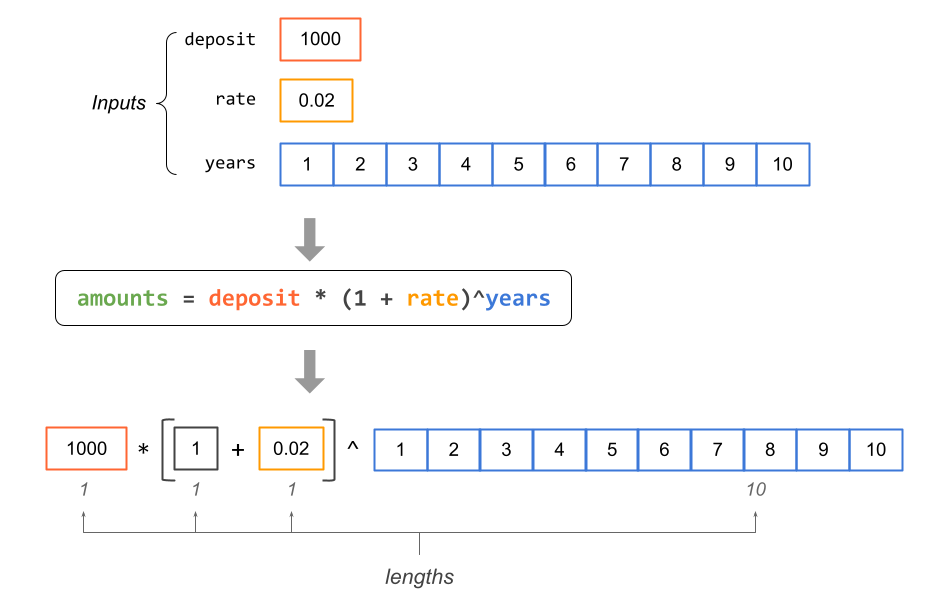
\includegraphics[width=0.9\linewidth]{images/vectors/vectorized1} 

}

\caption{Diagram depicting vectors of different lengths.}\label{fig:unnamed-chunk-77}
\end{figure}

How does R take care of this?

The following diagram depicts what R does behind the scenes: R recycles the
shorter vectors to match the length of the longest vector. In this example,
vectors \texttt{deposit}, \texttt{rate}, and \texttt{1} are the shorter vectors, which are then
recycle to match the length of the longest vector \texttt{years}. The computation
process is completed with vectorization.

\begin{center}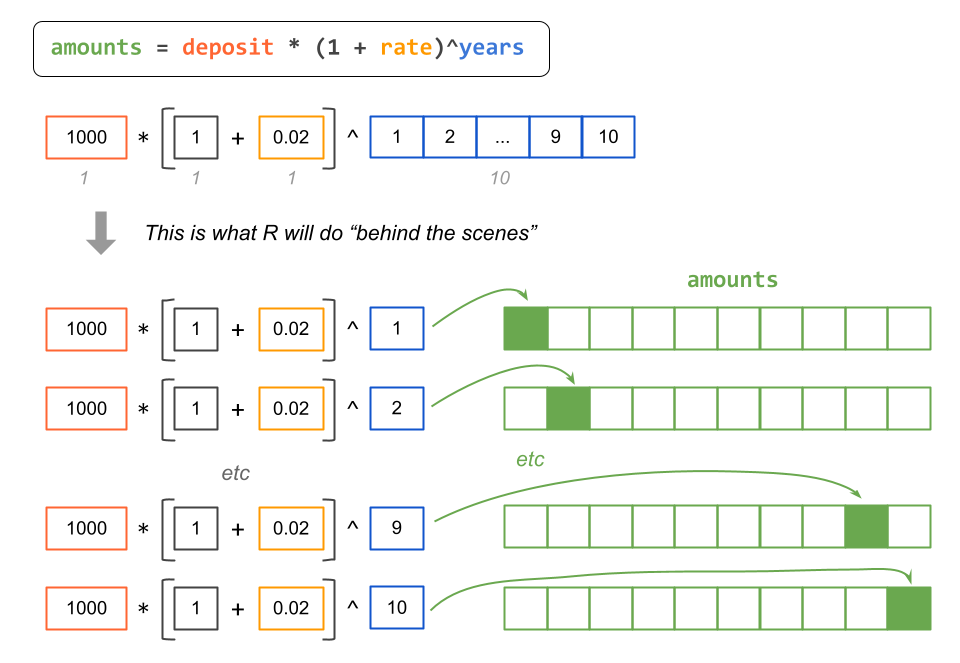
\includegraphics[width=0.9\linewidth]{images/vectors/vectorized2} \end{center}

As you can tell, this is an example of vectorization \& recycling rules in R.

\hypertarget{manipulating-vectors-subsetting}{%
\section{Manipulating Vectors: Subsetting}\label{manipulating-vectors-subsetting}}

In addition to creating vectors, you should also learn how to do some basic
manipulation of vectors. The most common type of manipulation is called
\emph{subsetting}, also known as \emph{indexing} or \emph{subscripting}, which we use to
extract and also replace elements of a vector (or another R object). To do so,
you use what I like to call \textbf{bracket notation}. This implies using (square)
brackets \texttt{{[}\ {]}} to get access to the elements of a vector.

To subset a vector, you type the name of the vector, followed by an opening
and a closing bracket. Inside the brackets you specify an indexing vector
which could be a numeric vector, a logical vector, and sometimes a character
vector. Let's see these options in more detail in the following subsections.

\begin{figure}

{\centering 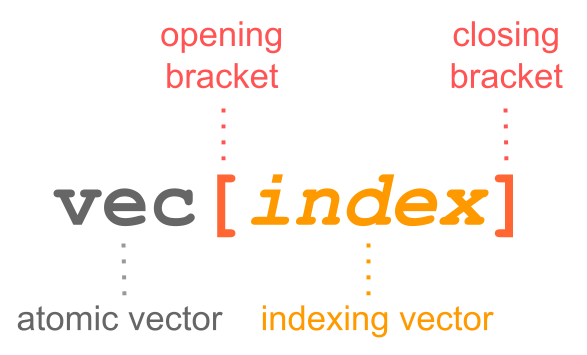
\includegraphics[width=0.45\linewidth]{images/vectors/obj-vector-brackets1} 

}

\caption{Use of brackets for subscripting vectors.}\label{fig:unnamed-chunk-79}
\end{figure}

\hypertarget{numeric-subsetting}{%
\subsection{Numeric Subsetting}\label{numeric-subsetting}}

This type of subsetting, as the name indicates, is when the indexing vector
consists of a numeric vector with one or more values that correspond to the
position(s) of the vector element(s).

The simplest type of numeric subsetting is when we use a single number (which
is a vector of length one).

\begin{Shaded}
\begin{Highlighting}[]
\CommentTok{\# amount at end of year 1}
\NormalTok{amounts[}\DecValTok{1}\NormalTok{]}
\SpecialCharTok{\textgreater{}}\NormalTok{ [}\DecValTok{1}\NormalTok{] }\DecValTok{1020}
\end{Highlighting}
\end{Shaded}

The numeric indexing vector can have more than one element. For example, if
we want to extract the elements in positions 1, 2 and 3, we could provide a
numeric sequence \texttt{1:3}:

\begin{Shaded}
\begin{Highlighting}[]
\CommentTok{\# amounts at end of years 1, 2, and 3}
\NormalTok{amounts[}\DecValTok{1}\SpecialCharTok{:}\DecValTok{3}\NormalTok{]}
\SpecialCharTok{\textgreater{}}\NormalTok{ [}\DecValTok{1}\NormalTok{] }\FloatTok{1020.000} \FloatTok{1040.400} \FloatTok{1061.208}
\end{Highlighting}
\end{Shaded}

The numeric positions don't have to be consecutive numbers. You can also use
a vector of non-consecutive numbers:

\begin{Shaded}
\begin{Highlighting}[]
\CommentTok{\# amounts at end of years 2 and 4}
\NormalTok{amounts[}\FunctionTok{c}\NormalTok{(}\DecValTok{2}\NormalTok{, }\DecValTok{4}\NormalTok{)]}
\SpecialCharTok{\textgreater{}}\NormalTok{ [}\DecValTok{1}\NormalTok{] }\FloatTok{1040.400} \FloatTok{1082.432}
\end{Highlighting}
\end{Shaded}

Likewise, we can also use a vector with repeated numbers:

\begin{Shaded}
\begin{Highlighting}[]
\CommentTok{\# repeated amounts}
\NormalTok{amounts[}\FunctionTok{c}\NormalTok{(}\DecValTok{2}\NormalTok{, }\DecValTok{2}\NormalTok{, }\DecValTok{2}\NormalTok{)]}
\SpecialCharTok{\textgreater{}}\NormalTok{ [}\DecValTok{1}\NormalTok{] }\FloatTok{1040.4} \FloatTok{1040.4} \FloatTok{1040.4}
\end{Highlighting}
\end{Shaded}

In addition to the previous subscripting options, we can specify negative
numbers to indicate that we want to exclude an element in the associated
position:

\begin{Shaded}
\begin{Highlighting}[]
\CommentTok{\# exclude 2nd year}
\NormalTok{amounts[}\SpecialCharTok{{-}}\DecValTok{2}\NormalTok{]}
\SpecialCharTok{\textgreater{}}\NormalTok{ [}\DecValTok{1}\NormalTok{] }\FloatTok{1020.000} \FloatTok{1061.208} \FloatTok{1082.432} \FloatTok{1104.081} \FloatTok{1126.162} \FloatTok{1148.686} \FloatTok{1171.659} \FloatTok{1195.093}
\SpecialCharTok{\textgreater{}}\NormalTok{ [}\DecValTok{9}\NormalTok{] }\FloatTok{1218.994}

\CommentTok{\# exclude 2nd and 4th years}
\NormalTok{amounts[}\SpecialCharTok{{-}}\FunctionTok{c}\NormalTok{(}\DecValTok{2}\NormalTok{, }\DecValTok{4}\NormalTok{)]}
\SpecialCharTok{\textgreater{}}\NormalTok{ [}\DecValTok{1}\NormalTok{] }\FloatTok{1020.000} \FloatTok{1061.208} \FloatTok{1104.081} \FloatTok{1126.162} \FloatTok{1148.686} \FloatTok{1171.659} \FloatTok{1195.093} \FloatTok{1218.994}
\end{Highlighting}
\end{Shaded}

\hypertarget{character-subsetting}{%
\subsection{Character Subsetting}\label{character-subsetting}}

Sometimes, you may have a vector with named elements. When this is the case,
you can use a character vector---containing one or more of the element names---as
the indexing vector.

None of the vectors that we have created so far have named elements. So let's
see how to do this. One way to give names to the elements of an existing vector
is with the function \texttt{names()}

\begin{Shaded}
\begin{Highlighting}[]
\NormalTok{amounts3 }\OtherTok{=}\NormalTok{ amounts[}\DecValTok{1}\SpecialCharTok{:}\DecValTok{3}\NormalTok{]}
\FunctionTok{names}\NormalTok{(amounts3) }\OtherTok{=} \FunctionTok{c}\NormalTok{(}\StringTok{"y1"}\NormalTok{, }\StringTok{"y2"}\NormalTok{, }\StringTok{"y3"}\NormalTok{)}
\NormalTok{amounts3}
\SpecialCharTok{\textgreater{}}\NormalTok{       y1       y2       y3 }
\SpecialCharTok{\textgreater{}} \FloatTok{1020.000} \FloatTok{1040.400} \FloatTok{1061.208}
\end{Highlighting}
\end{Shaded}

When a vector, like \texttt{amounts3}, has named elements, we can use those names for
subsetting purposes. Instead of using a numeric vector we use a character
vector. Hence the term \emph{character subsetting}.

For example, to extract the element in \texttt{amounts3} that has name \texttt{"y1"} we pass
this string inside the brackets:

\begin{Shaded}
\begin{Highlighting}[]
\NormalTok{amounts3[}\StringTok{"y1"}\NormalTok{]}
\SpecialCharTok{\textgreater{}}\NormalTok{   y1 }
\SpecialCharTok{\textgreater{}} \DecValTok{1020}
\end{Highlighting}
\end{Shaded}

To get the elements in \texttt{amounts3} that have names \texttt{"y1"} and \texttt{"y3"}, we can
write

\begin{Shaded}
\begin{Highlighting}[]
\NormalTok{amounts3[}\FunctionTok{c}\NormalTok{(}\StringTok{"y1"}\NormalTok{, }\StringTok{"y3"}\NormalTok{)]}
\SpecialCharTok{\textgreater{}}\NormalTok{       y1       y3 }
\SpecialCharTok{\textgreater{}} \FloatTok{1020.000} \FloatTok{1061.208}
\end{Highlighting}
\end{Shaded}

And like in the numeric subsetting case, we can also write a command such as:

\begin{Shaded}
\begin{Highlighting}[]
\NormalTok{amounts3[}\FunctionTok{c}\NormalTok{(}\StringTok{"y2"}\NormalTok{, }\StringTok{"y2"}\NormalTok{, }\StringTok{"y2"}\NormalTok{, }\StringTok{"y1"}\NormalTok{)]}
\SpecialCharTok{\textgreater{}}\NormalTok{     y2     y2     y2     y1 }
\SpecialCharTok{\textgreater{}} \FloatTok{1040.4} \FloatTok{1040.4} \FloatTok{1040.4} \FloatTok{1020.0}
\end{Highlighting}
\end{Shaded}

\hypertarget{logical-subsetting}{%
\subsection{Logical Subsetting}\label{logical-subsetting}}

Another type of subsetting is when we use a logical vector as the indexing
vector.

Let me show you an example of logical subsetting. In this case, we will use a
logical vector with three elements \texttt{c(TRUE,\ FALSE,\ FALSE)} and pass this
inside the brackets:

\begin{Shaded}
\begin{Highlighting}[]
\NormalTok{amounts3[}\FunctionTok{c}\NormalTok{(}\ConstantTok{TRUE}\NormalTok{, }\ConstantTok{FALSE}\NormalTok{, }\ConstantTok{FALSE}\NormalTok{)]}
\SpecialCharTok{\textgreater{}}\NormalTok{   y1 }
\SpecialCharTok{\textgreater{}} \DecValTok{1020}
\end{Highlighting}
\end{Shaded}

As you can tell, the retrieved element in \texttt{amounts3} is the one associated to
the \texttt{TRUE} position, whereas those elements associated to the \texttt{FALSE} values
are excluded. This is how the logical values (in the indexing vector) are used:

\begin{itemize}
\tightlist
\item
  \texttt{TRUE} means inclusion
\item
  \texttt{FALSE} means exclusion
\end{itemize}

So, if we want to extract only the element in the second position, we could
write something like this:

\begin{Shaded}
\begin{Highlighting}[]
\NormalTok{amounts3[}\FunctionTok{c}\NormalTok{(}\ConstantTok{FALSE}\NormalTok{, }\ConstantTok{TRUE}\NormalTok{, }\ConstantTok{FALSE}\NormalTok{)]}
\SpecialCharTok{\textgreater{}}\NormalTok{     y2 }
\SpecialCharTok{\textgreater{}} \FloatTok{1040.4}
\end{Highlighting}
\end{Shaded}

Now, I have to say that doing logical subsetting in this way is not really
how we tend to use it in practice. In other words, we won't be providing an
explicit logical vector, typing a bunch of \texttt{TRUE}'s and \texttt{FALSE}'s values.
Instead, what we typically do is to provide a command that, when executed by R,
will return a logical vector.

Consider the following example. We create a vector \texttt{x}, and then we use the
greater than symbol \texttt{\textgreater{}} to compute a mathematical comparison which in turn
will return a logical vector.

\begin{Shaded}
\begin{Highlighting}[]
\NormalTok{x }\OtherTok{=} \FunctionTok{c}\NormalTok{(}\DecValTok{2}\NormalTok{, }\DecValTok{4}\NormalTok{, }\DecValTok{6}\NormalTok{, }\DecValTok{8}\NormalTok{)}
\NormalTok{x }\SpecialCharTok{\textgreater{}} \DecValTok{5}
\SpecialCharTok{\textgreater{}}\NormalTok{ [}\DecValTok{1}\NormalTok{] }\ConstantTok{FALSE} \ConstantTok{FALSE}  \ConstantTok{TRUE}  \ConstantTok{TRUE}
\end{Highlighting}
\end{Shaded}

Knowing that \texttt{x\ \textgreater{}\ 5} produces a logical vector in which \texttt{FALSE} indicates that
the number is less than or equal 5, and \texttt{TRUE} indicates that the number
is greater than 5, we can write the following command to subset those
elements in \texttt{x} that are greater than five:

\begin{Shaded}
\begin{Highlighting}[]
\NormalTok{x[x }\SpecialCharTok{\textgreater{}} \DecValTok{5}\NormalTok{]}
\SpecialCharTok{\textgreater{}}\NormalTok{ [}\DecValTok{1}\NormalTok{] }\DecValTok{6} \DecValTok{8}
\end{Highlighting}
\end{Shaded}

This is a simple example of logical subsetting because the indexing vector
is the logical vector that comes from executing the comparison \texttt{x\ \textgreater{}\ 5}.

Here is a less simple example of logical subsetting to extract the elements in
\texttt{x} that are greater than 3 and less than or equal to 6. This requires\\
two comparison expressions, \texttt{x\ \textgreater{}\ 3} and \texttt{x\ \textless{}=\ 6}, and the use of the logical
\emph{AND} operator \texttt{\&} to form a compound logical comparison:

\begin{Shaded}
\begin{Highlighting}[]
\NormalTok{x[x }\SpecialCharTok{\textgreater{}} \DecValTok{3} \SpecialCharTok{\&}\NormalTok{ x }\SpecialCharTok{\textless{}=} \DecValTok{6}\NormalTok{]}
\SpecialCharTok{\textgreater{}}\NormalTok{ [}\DecValTok{1}\NormalTok{] }\DecValTok{4} \DecValTok{6}
\end{Highlighting}
\end{Shaded}

\hypertarget{summary-of-subsetting}{%
\subsection{Summary of Subsetting}\label{summary-of-subsetting}}

In summary, the things that you can specify inside the brackets are three
kind of vectors:

\begin{itemize}
\item
  numeric vectors
\item
  logical vectors (the length of the logical vector must match the length
  of the vector to be subset)
\item
  character vectors (if the elements have names)
\end{itemize}

In addition to the brackets \texttt{{[}{]}}, some common functions that you can use on
vectors are:

\begin{itemize}
\tightlist
\item
  \texttt{length()} gives the number of values
\item
  \texttt{sort()} sorts the values in increasing or decreasing ways
\item
  \texttt{rev()} reverses the values
\item
  \texttt{unique()} extracts unique elements
\end{itemize}

\begin{Shaded}
\begin{Highlighting}[]
\FunctionTok{length}\NormalTok{(amounts3)}
\NormalTok{amounts3[}\FunctionTok{length}\NormalTok{(amounts3)]}
\FunctionTok{sort}\NormalTok{(amounts3, }\AttributeTok{decreasing =} \ConstantTok{TRUE}\NormalTok{)}
\FunctionTok{rev}\NormalTok{(amounts3)}
\end{Highlighting}
\end{Shaded}

\begin{center}\rule{0.5\linewidth}{0.5pt}\end{center}

\hypertarget{exercises-3}{%
\section{Exercises}\label{exercises-3}}

\textbf{1)} Explain, in your own words, the concept of \emph{vectorization} a.k.a.
vectorized operations in R.

\textbf{2)} Explain, in your own words, the \emph{recycling principle} in R.

\textbf{3)} Write 2 different R commands to return the first five elements of a
vector \texttt{x} (assume \texttt{x} has more than 5 elements).

\textbf{4)} Suppose \texttt{y\ \textless{}-\ c(1,\ 4,\ 9,\ 16,\ 25)}. Write down the R command to return a
vector \texttt{z}, in which each element of \texttt{z} is the square root of each element of
the vector \texttt{y}.

\textbf{5)} Which command will fail to return the first five elements of a vector
\texttt{x}? (assume \texttt{x} has more than 5 elements).

\begin{enumerate}
\def\labelenumi{\alph{enumi})}
\item
  \texttt{x{[}1:5{]}}
\item
  \texttt{x{[}c(1,2,3,4,5){]}}
\item
  \texttt{head(x,\ n\ =\ 5)}
\item
  \texttt{x{[}seq(1,\ 5){]}}
\item
  \texttt{x(1:5)}
\end{enumerate}

\textbf{6)} For each the following parts, state whether the given function or
operator is vectorized, and provide a code example to support your claim.

\begin{enumerate}
\def\labelenumi{\alph{enumi})}
\item
  \texttt{length()}
\item
  \texttt{*}
\item
  \texttt{log()}
\item
  \texttt{max()}
\item
  \texttt{trunc()}
\end{enumerate}

\textbf{7)} Consider the following code to obtain vectors \texttt{name} and \texttt{mpg} from the
data set \texttt{mtcars} that contains data about 32 automobiles (1973--74 models).

\begin{Shaded}
\begin{Highlighting}[]
\CommentTok{\# vectors name and mpg}
\NormalTok{name }\OtherTok{=} \FunctionTok{rownames}\NormalTok{(mtcars)}
\NormalTok{mpg }\OtherTok{=}\NormalTok{ mtcars}\SpecialCharTok{$}\NormalTok{mpg}
\end{Highlighting}
\end{Shaded}

Use \texttt{seq()}, and bracket notation, to subset (extract):

\begin{enumerate}
\def\labelenumi{\alph{enumi})}
\item
  all the even elements in \texttt{name} (i.e.~extract positions 2, 4, 6, etc)
\item
  all the odd elements in \texttt{mpg} (i.e.~extract positions 1, 3, 5, etc)
\item
  all the elements in positions multiples of 5 (e.g.~extract positions 5, 10,
  15, etc) of \texttt{mpg}
\item
  all the even elements in \texttt{name} but this time in reverse order; \emph{hint} the
  \texttt{rev()} function is your friend.
\end{enumerate}

\textbf{8)} Consider the following code to obtain vectors \texttt{name}, \texttt{mpg} and \texttt{cyl}
from the data set \texttt{mtcars} that contains data about 32 automobiles (1973--74
models).

\begin{Shaded}
\begin{Highlighting}[]
\CommentTok{\# vectors name, mpg and cyl}
\NormalTok{name }\OtherTok{=} \FunctionTok{rownames}\NormalTok{(mtcars)}
\NormalTok{mpg }\OtherTok{=}\NormalTok{ mtcars}\SpecialCharTok{$}\NormalTok{mpg }\CommentTok{\# miles{-}per{-}gallon}
\NormalTok{cyl }\OtherTok{=}\NormalTok{ mtcars}\SpecialCharTok{$}\NormalTok{cyl  }\CommentTok{\# number of cylinders}
\end{Highlighting}
\end{Shaded}

Write commands, using bracket notation, to answer the parts listed below.
You may need to use \texttt{is.na()}, \texttt{sum()}, \texttt{min()}, \texttt{max()}, \texttt{which()},
\texttt{which.min()}, \texttt{which.max()}:

\begin{enumerate}
\def\labelenumi{\alph{enumi})}
\item
  name of cars that have a fuel consumption of less than 15 mpg
\item
  name of cars that have 6 cylinders
\item
  largest mpg value of all cars with 8 cylinders
\item
  name of car(s) with mpg equal to the median mpg
\item
  name of car(s) with mpg of at most 22, and at least 6 cylinders
\end{enumerate}

\hypertarget{part-more-atomic-objects}{%
\part{More Atomic Objects}\label{part-more-atomic-objects}}

\hypertarget{factors}{%
\chapter{Factors}\label{factors}}

I'm one of those with the humble opinion that great software for data science
and analytics should have a data structure dedicated to handle categorical data.
Luckily, one of the nicest features about R is that it provides a data
object exclusively designed to handle categorical data: \textbf{factors}.

The term ``factor'' as used in R for handling categorical variables, comes from
the terminology used in \emph{Analysis of Variance}, commonly referred to as ANOVA.
In this statistical method, a categorical variable is commonly referred to as,
surprise-surprise, \emph{factor} and its categories are known as \emph{levels}. Perhaps
this is not the best terminology but it is the one R uses, which reflects its
distinctive statistical origins. Especially for those users without a background
in statistics, this is one of R's idiosyncrasies that seems disconcerting at
the beginning. But as long as you keep in mind that a factor is just the object
that allows you to handle a qualitative variable you'll be fine. In case you
need it, here's a short mantra to remember:

\begin{quote}
factors have levels
\end{quote}

\hypertarget{creating-factors}{%
\section{Creating Factors}\label{creating-factors}}

To create a factor in R you use the homonym function \texttt{factor()}, which takes a
vector as input. The vector can be either numeric, character or logical. Let's
see our first example:

\begin{Shaded}
\begin{Highlighting}[]
\CommentTok{\# numeric vector}
\NormalTok{num\_vector }\OtherTok{\textless{}{-}} \FunctionTok{c}\NormalTok{(}\DecValTok{1}\NormalTok{, }\DecValTok{2}\NormalTok{, }\DecValTok{3}\NormalTok{, }\DecValTok{1}\NormalTok{, }\DecValTok{2}\NormalTok{, }\DecValTok{3}\NormalTok{, }\DecValTok{2}\NormalTok{)}

\CommentTok{\# creating a factor from num\_vector}
\NormalTok{first\_factor }\OtherTok{\textless{}{-}} \FunctionTok{factor}\NormalTok{(num\_vector)}

\NormalTok{first\_factor}
\SpecialCharTok{\textgreater{}}\NormalTok{ [}\DecValTok{1}\NormalTok{] }\DecValTok{1} \DecValTok{2} \DecValTok{3} \DecValTok{1} \DecValTok{2} \DecValTok{3} \DecValTok{2}
\SpecialCharTok{\textgreater{}}\NormalTok{ Levels}\SpecialCharTok{:} \DecValTok{1} \DecValTok{2} \DecValTok{3}
\end{Highlighting}
\end{Shaded}

As you can tell from the previous code snippet, \texttt{factor()} converts the numeric
vector \texttt{num\_vector} into a factor (i.e.~a categorical variable) with 3
categories---the so called \texttt{levels}.

You can also obtain a factor from a string vector:

\begin{Shaded}
\begin{Highlighting}[]
\CommentTok{\# string vector}
\NormalTok{str\_vector }\OtherTok{\textless{}{-}} \FunctionTok{c}\NormalTok{(}\StringTok{\textquotesingle{}a\textquotesingle{}}\NormalTok{, }\StringTok{\textquotesingle{}b\textquotesingle{}}\NormalTok{, }\StringTok{\textquotesingle{}c\textquotesingle{}}\NormalTok{, }\StringTok{\textquotesingle{}b\textquotesingle{}}\NormalTok{, }\StringTok{\textquotesingle{}c\textquotesingle{}}\NormalTok{, }\StringTok{\textquotesingle{}a\textquotesingle{}}\NormalTok{, }\StringTok{\textquotesingle{}c\textquotesingle{}}\NormalTok{, }\StringTok{\textquotesingle{}b\textquotesingle{}}\NormalTok{)}

\NormalTok{str\_vector}
\SpecialCharTok{\textgreater{}}\NormalTok{ [}\DecValTok{1}\NormalTok{] }\StringTok{"a"} \StringTok{"b"} \StringTok{"c"} \StringTok{"b"} \StringTok{"c"} \StringTok{"a"} \StringTok{"c"} \StringTok{"b"}

\CommentTok{\# creating a factor from str\_vector}
\NormalTok{second\_factor }\OtherTok{\textless{}{-}} \FunctionTok{factor}\NormalTok{(str\_vector)}

\NormalTok{second\_factor}
\SpecialCharTok{\textgreater{}}\NormalTok{ [}\DecValTok{1}\NormalTok{] a b c b c a c b}
\SpecialCharTok{\textgreater{}}\NormalTok{ Levels}\SpecialCharTok{:}\NormalTok{ a b c}
\end{Highlighting}
\end{Shaded}

Notice how \texttt{str\_vector} and \texttt{second\_factor} are displayed. Even though the
elements are the same in both the vector and the factor, they are printed in
different formats. The letters in the string vector are displayed with quotes,
while the letters in the factor are printed without quotes.

And of course, you can use a logical vector to generate a factor as well:

\begin{Shaded}
\begin{Highlighting}[]
\CommentTok{\# logical vector}
\NormalTok{log\_vector }\OtherTok{\textless{}{-}} \FunctionTok{c}\NormalTok{(}\ConstantTok{TRUE}\NormalTok{, }\ConstantTok{FALSE}\NormalTok{, }\ConstantTok{TRUE}\NormalTok{, }\ConstantTok{TRUE}\NormalTok{, }\ConstantTok{FALSE}\NormalTok{)}

\CommentTok{\# creating a factor from log\_vector}
\NormalTok{third\_factor }\OtherTok{\textless{}{-}} \FunctionTok{factor}\NormalTok{(log\_vector)}

\NormalTok{third\_factor}
\SpecialCharTok{\textgreater{}}\NormalTok{ [}\DecValTok{1}\NormalTok{] }\ConstantTok{TRUE}  \ConstantTok{FALSE} \ConstantTok{TRUE}  \ConstantTok{TRUE}  \ConstantTok{FALSE}
\SpecialCharTok{\textgreater{}}\NormalTok{ Levels}\SpecialCharTok{:} \ConstantTok{FALSE} \ConstantTok{TRUE}
\end{Highlighting}
\end{Shaded}

\hypertarget{how-r-treats-factors}{%
\section{How R treats factors}\label{how-r-treats-factors}}

Technically speaking, R factors are referred to as \emph{compound objects}. According
to the ``R Language Definition'' manual:

\begin{quote}
``Factors are currently implemented using an integer array to specify the
actual levels and a second array of names that are mapped to the integers.''
\end{quote}

What does this mean?

Essentially, a factor is internally stored using two ingredients: one is an
integer vector containing the values of categories, the other is a vector with
the ``levels'' which has the names of categories which are mapped to the integers.

Under the hood, the way R stores factors is as vectors of integer values.
One way to confirm this is using the function \texttt{storage.mode()}

\begin{Shaded}
\begin{Highlighting}[]
\CommentTok{\# storage of factor}
\FunctionTok{storage.mode}\NormalTok{(first\_factor)}
\SpecialCharTok{\textgreater{}}\NormalTok{ [}\DecValTok{1}\NormalTok{] }\StringTok{"integer"}
\end{Highlighting}
\end{Shaded}

This means that we can manipulate factors just like we manipulate vectors. In
addition, many functions for vectors can be applied to factors. For instance,
we can use the function \texttt{length()} to get the number of elements in a factor:

\begin{Shaded}
\begin{Highlighting}[]
\CommentTok{\# factors have length}
\FunctionTok{length}\NormalTok{(first\_factor)}
\SpecialCharTok{\textgreater{}}\NormalTok{ [}\DecValTok{1}\NormalTok{] }\DecValTok{7}
\end{Highlighting}
\end{Shaded}

We can also use the square brackets \texttt{{[}\ {]}} to extract or select elements of a
factor. Inside the brackets we specify vectors of indices such as numeric
vectors, logical vectors, and sometimes even character vectors.

\begin{Shaded}
\begin{Highlighting}[]
\CommentTok{\# first element}
\NormalTok{first\_factor[}\DecValTok{1}\NormalTok{]}

\CommentTok{\# third element}
\NormalTok{first\_factor[}\DecValTok{3}\NormalTok{]}

\CommentTok{\# second to fourth elements}
\NormalTok{first\_factor[}\DecValTok{2}\SpecialCharTok{:}\DecValTok{4}\NormalTok{]}

\CommentTok{\# last element}
\NormalTok{first\_factor[}\FunctionTok{length}\NormalTok{(first\_factor)]}

\CommentTok{\# logical subsetting}
\NormalTok{first\_factor[}\FunctionTok{rep}\NormalTok{(}\FunctionTok{c}\NormalTok{(}\ConstantTok{TRUE}\NormalTok{, }\ConstantTok{FALSE}\NormalTok{), }\AttributeTok{length.out =} \DecValTok{7}\NormalTok{)]}
\end{Highlighting}
\end{Shaded}

If you have a factor with named elements, you can also specify the names of
the elements within the brackets:

\begin{Shaded}
\begin{Highlighting}[]
\FunctionTok{names}\NormalTok{(first\_factor) }\OtherTok{\textless{}{-}}\NormalTok{ letters[}\DecValTok{1}\SpecialCharTok{:}\FunctionTok{length}\NormalTok{(first\_factor)]}
\NormalTok{first\_factor}
\SpecialCharTok{\textgreater{}}\NormalTok{ a b c d e f g }
\SpecialCharTok{\textgreater{}} \DecValTok{1} \DecValTok{2} \DecValTok{3} \DecValTok{1} \DecValTok{2} \DecValTok{3} \DecValTok{2} 
\SpecialCharTok{\textgreater{}}\NormalTok{ Levels}\SpecialCharTok{:} \DecValTok{1} \DecValTok{2} \DecValTok{3}

\NormalTok{first\_factor[}\FunctionTok{c}\NormalTok{(}\StringTok{\textquotesingle{}b\textquotesingle{}}\NormalTok{, }\StringTok{\textquotesingle{}d\textquotesingle{}}\NormalTok{, }\StringTok{\textquotesingle{}f\textquotesingle{}}\NormalTok{)]}
\SpecialCharTok{\textgreater{}}\NormalTok{ b d f }
\SpecialCharTok{\textgreater{}} \DecValTok{2} \DecValTok{1} \DecValTok{3} 
\SpecialCharTok{\textgreater{}}\NormalTok{ Levels}\SpecialCharTok{:} \DecValTok{1} \DecValTok{2} \DecValTok{3}
\end{Highlighting}
\end{Shaded}

However, you should know that factors are NOT really vectors. To see this you
can check the behavior of the functions \texttt{is.factor()} and \texttt{is.vector()} on a
factor:

\begin{Shaded}
\begin{Highlighting}[]
\CommentTok{\# factors are not vectors}
\FunctionTok{is.vector}\NormalTok{(first\_factor)}
\SpecialCharTok{\textgreater{}}\NormalTok{ [}\DecValTok{1}\NormalTok{] }\ConstantTok{FALSE}

\CommentTok{\# factors are factors}
\FunctionTok{is.factor}\NormalTok{(first\_factor)}
\SpecialCharTok{\textgreater{}}\NormalTok{ [}\DecValTok{1}\NormalTok{] }\ConstantTok{TRUE}
\end{Highlighting}
\end{Shaded}

Even a single element of a factor is also a factor:

\begin{Shaded}
\begin{Highlighting}[]
\FunctionTok{class}\NormalTok{(first\_factor[}\DecValTok{1}\NormalTok{])}
\SpecialCharTok{\textgreater{}}\NormalTok{ [}\DecValTok{1}\NormalTok{] }\StringTok{"factor"}
\end{Highlighting}
\end{Shaded}

\hypertarget{so-what-makes-a-factor-different-from-a-vector}{%
\subsubsection*{So what makes a factor different from a vector?}\label{so-what-makes-a-factor-different-from-a-vector}}
\addcontentsline{toc}{subsubsection}{So what makes a factor different from a vector?}

Well, it turns out that factors have an additional attribute that vectors don't:
\texttt{levels}. And as you can expect, the class of a factor is indeed \texttt{"factor"}
(not \texttt{"vector"}).

\begin{Shaded}
\begin{Highlighting}[]
\CommentTok{\# attributes of a factor}
\FunctionTok{attributes}\NormalTok{(first\_factor)}
\SpecialCharTok{\textgreater{}} \ErrorTok{$}\NormalTok{levels}
\SpecialCharTok{\textgreater{}}\NormalTok{ [}\DecValTok{1}\NormalTok{] }\StringTok{"1"} \StringTok{"2"} \StringTok{"3"}
\SpecialCharTok{\textgreater{}} 
\ErrorTok{\textgreater{}} \ErrorTok{$}\NormalTok{class}
\SpecialCharTok{\textgreater{}}\NormalTok{ [}\DecValTok{1}\NormalTok{] }\StringTok{"factor"}
\SpecialCharTok{\textgreater{}} 
\ErrorTok{\textgreater{}} \ErrorTok{$}\NormalTok{names}
\SpecialCharTok{\textgreater{}}\NormalTok{ [}\DecValTok{1}\NormalTok{] }\StringTok{"a"} \StringTok{"b"} \StringTok{"c"} \StringTok{"d"} \StringTok{"e"} \StringTok{"f"} \StringTok{"g"}
\end{Highlighting}
\end{Shaded}

Another feature that makes factors so special is that their values (the levels)
are mapped to a set of character values for displaying purposes. This might
seem like a minor feature but it has two important consequences. On the one
hand, this implies that factors provide a way to store character values very
efficiently. Why? Because each unique character value is stored only once, and
the data itself is stored as a vector of integers.

Notice how the numeric value \texttt{1} was mapped into the character value \texttt{"1"}. And
the same happens for the other values \texttt{2} and \texttt{3} that are mapped into the
characters \texttt{"2"} and \texttt{"3"}.

\hypertarget{what-is-the-advantage-of-r-factors}{%
\subsubsection*{What is the advantage of R factors?}\label{what-is-the-advantage-of-r-factors}}
\addcontentsline{toc}{subsubsection}{What is the advantage of R factors?}

Every time I teach about factors, there is inevitably one student who asks a
very pertinent question: Why do we want to use factors? Isn't it redundant to
have a factor object when there are already character or integer vectors?

I have two answers to this question.

The first has to do with the storage of factors. Storing a factor as integers
will usually be more efficient than storing a character vector. As we've seen,
this is an important issue especially when the data---to be encoded into a
factor---is of considerable size.

The second reason has to do with categorical variables of \emph{ordinal} nature.
Qualitative data can be classified into nominal and ordinal variables. Nominal
variables could be easily handled with character vectors. In fact, \emph{nominal}
means name (values are just names or labels), and there's no natural order
among the categories.

A different story is when we have ordinal variables, like sizes \texttt{"small"},
\texttt{"medium"}, \texttt{"large"} or college years \texttt{"freshman"}, \texttt{"sophomore"}, \texttt{"junior"},
\texttt{"senior"}. In these cases we are still using names of categories, but they
can be arranged in increasing or decreasing order. In other words, we can rank
the categories since they have a natural order: small is less than medium which
is less than large. Likewise, freshman comes first, then sophomore, followed by
junior, and finally senior.

So here's an important question: How do we keep the order of categories in an
ordinal variable? We can use a character vector to store the values. But a
character vector does not allow us to store the ranking of categories. The
solution in R comes via factors. We can use factors to define ordinal variables,
like the following example:

\begin{Shaded}
\begin{Highlighting}[]
\NormalTok{sizes }\OtherTok{\textless{}{-}} \FunctionTok{factor}\NormalTok{(}
  \AttributeTok{x =} \FunctionTok{c}\NormalTok{(}\StringTok{\textquotesingle{}sm\textquotesingle{}}\NormalTok{, }\StringTok{\textquotesingle{}md\textquotesingle{}}\NormalTok{, }\StringTok{\textquotesingle{}lg\textquotesingle{}}\NormalTok{, }\StringTok{\textquotesingle{}sm\textquotesingle{}}\NormalTok{, }\StringTok{\textquotesingle{}md\textquotesingle{}}\NormalTok{),}
  \AttributeTok{levels =} \FunctionTok{c}\NormalTok{(}\StringTok{\textquotesingle{}sm\textquotesingle{}}\NormalTok{, }\StringTok{\textquotesingle{}md\textquotesingle{}}\NormalTok{, }\StringTok{\textquotesingle{}lg\textquotesingle{}}\NormalTok{),}
  \AttributeTok{ordered =} \ConstantTok{TRUE}\NormalTok{)}

\NormalTok{sizes}
\SpecialCharTok{\textgreater{}}\NormalTok{ [}\DecValTok{1}\NormalTok{] sm md lg sm md}
\SpecialCharTok{\textgreater{}}\NormalTok{ Levels}\SpecialCharTok{:}\NormalTok{ sm }\SpecialCharTok{\textless{}}\NormalTok{ md }\SpecialCharTok{\textless{}}\NormalTok{ lg}
\end{Highlighting}
\end{Shaded}

As you can tell, \texttt{sizes} has ordered levels, clearly identifying the first
category \texttt{"sm"}, the second one \texttt{"md"}, and the third one \texttt{"lg"}.

\hypertarget{a-closer-look-at-factor}{%
\section{\texorpdfstring{A closer look at \texttt{factor()}}{A closer look at factor()}}\label{a-closer-look-at-factor}}

Since working with categorical data in R typically involves working with factors,
you should become familiar with the variety of functions related with them. In
the following sections we'll cover a bunch of details about factors so you can
be better prepared to deal with any type of categorical data.

\hypertarget{function-factor}{%
\subsection{\texorpdfstring{Function \texttt{factor()}}{Function factor()}}\label{function-factor}}

Given the fundamental role played by the function \texttt{factor()} we need to pay a
closer look at its arguments. If you check the documentation---see
\texttt{help(factor)}---you'll see that the usage of the function \texttt{factor()} is:

\begin{verbatim}
  factor(x = character(), levels, labels = levels,
         exclude = NA, ordered = is.ordered(x), nmax = NA)
\end{verbatim}

with the following arguments:

\begin{itemize}
\item
  \texttt{x} a vector of data
\item
  \texttt{levels} an optional vector for the categories
\item
  \texttt{labels} an optional character vector of labels for the levels
\item
  \texttt{exclude} a vector of values to be excluded when forming the set of levels
\item
  \texttt{ordered} logical value to indicate if the levels should be regarded as ordered
\item
  \texttt{nmax} an upper bound on the number of levels
\end{itemize}

The main argument of \texttt{factor()} is the input vector \texttt{x}. The next argument is
\texttt{levels}, followed by \texttt{labels}, both of which are optional arguments. Although
you won't always be providing values for \texttt{levels} and \texttt{labels}, it is important
to understand how R handles these arguments by default.

\hypertarget{argument-levels}{%
\subsubsection*{\texorpdfstring{Argument \texttt{levels}}{Argument levels}}\label{argument-levels}}
\addcontentsline{toc}{subsubsection}{Argument \texttt{levels}}

If \texttt{levels} is not provided (which is what happens in most cases), then R
assigns the unique values in \texttt{x} as the category levels.

For example, consider our numeric vector from the first example: \texttt{num\_vector}
contains unique values 1, 2, and 3.

\begin{Shaded}
\begin{Highlighting}[]
\CommentTok{\# numeric vector}
\NormalTok{num\_vector }\OtherTok{\textless{}{-}} \FunctionTok{c}\NormalTok{(}\DecValTok{1}\NormalTok{, }\DecValTok{2}\NormalTok{, }\DecValTok{3}\NormalTok{, }\DecValTok{1}\NormalTok{, }\DecValTok{2}\NormalTok{, }\DecValTok{3}\NormalTok{, }\DecValTok{2}\NormalTok{)}

\CommentTok{\# creating a factor from num\_vector}
\NormalTok{first\_factor }\OtherTok{\textless{}{-}} \FunctionTok{factor}\NormalTok{(num\_vector)}

\NormalTok{first\_factor}
\SpecialCharTok{\textgreater{}}\NormalTok{ [}\DecValTok{1}\NormalTok{] }\DecValTok{1} \DecValTok{2} \DecValTok{3} \DecValTok{1} \DecValTok{2} \DecValTok{3} \DecValTok{2}
\SpecialCharTok{\textgreater{}}\NormalTok{ Levels}\SpecialCharTok{:} \DecValTok{1} \DecValTok{2} \DecValTok{3}
\end{Highlighting}
\end{Shaded}

Now imagine we want to have \texttt{levels} 1, 2, 3, 4, and 5. This is how you can
define the factor with an extended set of levels:

\begin{Shaded}
\begin{Highlighting}[]
\CommentTok{\# numeric vector}
\NormalTok{num\_vector}
\SpecialCharTok{\textgreater{}}\NormalTok{ [}\DecValTok{1}\NormalTok{] }\DecValTok{1} \DecValTok{2} \DecValTok{3} \DecValTok{1} \DecValTok{2} \DecValTok{3} \DecValTok{2}

\CommentTok{\# defining levels}
\NormalTok{one\_factor }\OtherTok{\textless{}{-}} \FunctionTok{factor}\NormalTok{(num\_vector, }\AttributeTok{levels =} \DecValTok{1}\SpecialCharTok{:}\DecValTok{5}\NormalTok{)}
\NormalTok{one\_factor}
\SpecialCharTok{\textgreater{}}\NormalTok{ [}\DecValTok{1}\NormalTok{] }\DecValTok{1} \DecValTok{2} \DecValTok{3} \DecValTok{1} \DecValTok{2} \DecValTok{3} \DecValTok{2}
\SpecialCharTok{\textgreater{}}\NormalTok{ Levels}\SpecialCharTok{:} \DecValTok{1} \DecValTok{2} \DecValTok{3} \DecValTok{4} \DecValTok{5}
\end{Highlighting}
\end{Shaded}

Although the created factor only has values between 1 and 3, the \texttt{levels} range
from 1 to 5. This can be useful if we plan to add elements whose values are not
in the input vector \texttt{num\_vector}. For instance, you can append two more elements
to \texttt{one\_factor} with values \texttt{4} and \texttt{5} like this:

\begin{Shaded}
\begin{Highlighting}[]
\CommentTok{\# adding values 4 and 5}
\NormalTok{one\_factor[}\FunctionTok{c}\NormalTok{(}\DecValTok{8}\NormalTok{, }\DecValTok{9}\NormalTok{)] }\OtherTok{\textless{}{-}} \FunctionTok{c}\NormalTok{(}\DecValTok{4}\NormalTok{, }\DecValTok{5}\NormalTok{)}
\NormalTok{one\_factor}
\SpecialCharTok{\textgreater{}}\NormalTok{ [}\DecValTok{1}\NormalTok{] }\DecValTok{1} \DecValTok{2} \DecValTok{3} \DecValTok{1} \DecValTok{2} \DecValTok{3} \DecValTok{2} \DecValTok{4} \DecValTok{5}
\SpecialCharTok{\textgreater{}}\NormalTok{ Levels}\SpecialCharTok{:} \DecValTok{1} \DecValTok{2} \DecValTok{3} \DecValTok{4} \DecValTok{5}
\end{Highlighting}
\end{Shaded}

If you attempt to insert an element having a value that is not in the
predefined set of levels, R will insert a missing value (\texttt{\textless{}NA\textgreater{}}) instead, and
you'll get a warning message like the one below:

\begin{Shaded}
\begin{Highlighting}[]
\CommentTok{\# attempting to add value 6 (not in levels)}
\NormalTok{one\_factor[}\DecValTok{1}\NormalTok{] }\OtherTok{\textless{}{-}} \DecValTok{6}
\SpecialCharTok{\textgreater{}}\NormalTok{ Warning }\ControlFlowTok{in} \StringTok{\textasciigrave{}}\AttributeTok{[\textless{}{-}.factor}\StringTok{\textasciigrave{}}\NormalTok{(}\StringTok{\textasciigrave{}}\AttributeTok{*tmp*}\StringTok{\textasciigrave{}}\NormalTok{, }\DecValTok{1}\NormalTok{, }\AttributeTok{value =} \DecValTok{6}\NormalTok{)}\SpecialCharTok{:}\NormalTok{ invalid factor level, }\ConstantTok{NA}
\SpecialCharTok{\textgreater{}}\NormalTok{ generated}
\NormalTok{one\_factor}
\SpecialCharTok{\textgreater{}}\NormalTok{ [}\DecValTok{1}\NormalTok{] }\SpecialCharTok{\textless{}}\ConstantTok{NA}\SpecialCharTok{\textgreater{}} \DecValTok{2}    \DecValTok{3}    \DecValTok{1}    \DecValTok{2}    \DecValTok{3}    \DecValTok{2}    \DecValTok{4}    \DecValTok{5}   
\SpecialCharTok{\textgreater{}}\NormalTok{ Levels}\SpecialCharTok{:} \DecValTok{1} \DecValTok{2} \DecValTok{3} \DecValTok{4} \DecValTok{5}
\end{Highlighting}
\end{Shaded}

\hypertarget{argument-labels}{%
\subsubsection*{\texorpdfstring{Argument \texttt{labels}}{Argument labels}}\label{argument-labels}}
\addcontentsline{toc}{subsubsection}{Argument \texttt{labels}}

Another very useful argument is \texttt{labels}, which allows you to provide a string
vector for naming the \texttt{levels} in a different way from the values in \texttt{x}. Let's
take the numeric vector \texttt{num\_vector} again, and say we want to use words as
labels instead of numeric values. Here's how you can create a factor with
predefined \texttt{labels}:

\begin{Shaded}
\begin{Highlighting}[]
\CommentTok{\# defining labels}
\NormalTok{num\_word\_vector }\OtherTok{\textless{}{-}} \FunctionTok{factor}\NormalTok{(num\_vector, }\AttributeTok{labels =} \FunctionTok{c}\NormalTok{(}\StringTok{"one"}\NormalTok{, }\StringTok{"two"}\NormalTok{, }\StringTok{"three"}\NormalTok{))}

\NormalTok{num\_word\_vector}
\SpecialCharTok{\textgreater{}}\NormalTok{ [}\DecValTok{1}\NormalTok{] one   two   three one   two   three two  }
\SpecialCharTok{\textgreater{}}\NormalTok{ Levels}\SpecialCharTok{:}\NormalTok{ one two three}
\end{Highlighting}
\end{Shaded}

\hypertarget{argument-exclude}{%
\subsubsection*{\texorpdfstring{Argument \texttt{exclude}}{Argument exclude}}\label{argument-exclude}}
\addcontentsline{toc}{subsubsection}{Argument \texttt{exclude}}

If you want to ignore some values of the input vector \texttt{x}, you can use the
\texttt{exclude} argument. You just need to provide those values which will be removed
from the set of \texttt{levels}.

\begin{Shaded}
\begin{Highlighting}[]
\CommentTok{\# excluding level 3}
\FunctionTok{factor}\NormalTok{(num\_vector, }\AttributeTok{exclude =} \DecValTok{3}\NormalTok{)}
\SpecialCharTok{\textgreater{}}\NormalTok{ [}\DecValTok{1}\NormalTok{] }\DecValTok{1}    \DecValTok{2}    \SpecialCharTok{\textless{}}\ConstantTok{NA}\SpecialCharTok{\textgreater{}} \DecValTok{1}    \DecValTok{2}    \SpecialCharTok{\textless{}}\ConstantTok{NA}\SpecialCharTok{\textgreater{}} \DecValTok{2}   
\SpecialCharTok{\textgreater{}}\NormalTok{ Levels}\SpecialCharTok{:} \DecValTok{1} \DecValTok{2}

\CommentTok{\# excluding levels 1 and 3}
\FunctionTok{factor}\NormalTok{(num\_vector, }\AttributeTok{exclude =} \FunctionTok{c}\NormalTok{(}\DecValTok{1}\NormalTok{,}\DecValTok{3}\NormalTok{))}
\SpecialCharTok{\textgreater{}}\NormalTok{ [}\DecValTok{1}\NormalTok{] }\SpecialCharTok{\textless{}}\ConstantTok{NA}\SpecialCharTok{\textgreater{}} \DecValTok{2}    \SpecialCharTok{\textless{}}\ConstantTok{NA}\SpecialCharTok{\textgreater{}} \ErrorTok{\textless{}}\ConstantTok{NA}\SpecialCharTok{\textgreater{}} \DecValTok{2}    \SpecialCharTok{\textless{}}\ConstantTok{NA}\SpecialCharTok{\textgreater{}} \DecValTok{2}   
\SpecialCharTok{\textgreater{}}\NormalTok{ Levels}\SpecialCharTok{:} \DecValTok{2}
\end{Highlighting}
\end{Shaded}

The side effect of \texttt{exclude} is that it returns a missing value (\texttt{\textless{}NA\textgreater{}}) for
each element that was excluded, which is not always what we want. Here's one
way to remove the missing values when excluding 3:

\begin{Shaded}
\begin{Highlighting}[]
\CommentTok{\# excluding level 3}
\NormalTok{num\_fac12 }\OtherTok{\textless{}{-}} \FunctionTok{factor}\NormalTok{(num\_vector, }\AttributeTok{exclude =} \DecValTok{3}\NormalTok{)}

\CommentTok{\# oops, we have some missing values}
\NormalTok{num\_fac12}
\SpecialCharTok{\textgreater{}}\NormalTok{ [}\DecValTok{1}\NormalTok{] }\DecValTok{1}    \DecValTok{2}    \SpecialCharTok{\textless{}}\ConstantTok{NA}\SpecialCharTok{\textgreater{}} \DecValTok{1}    \DecValTok{2}    \SpecialCharTok{\textless{}}\ConstantTok{NA}\SpecialCharTok{\textgreater{}} \DecValTok{2}   
\SpecialCharTok{\textgreater{}}\NormalTok{ Levels}\SpecialCharTok{:} \DecValTok{1} \DecValTok{2}
\CommentTok{\# removing missing values}
\NormalTok{num\_fac12[}\SpecialCharTok{!}\FunctionTok{is.na}\NormalTok{(num\_fac12)]}
\SpecialCharTok{\textgreater{}}\NormalTok{ [}\DecValTok{1}\NormalTok{] }\DecValTok{1} \DecValTok{2} \DecValTok{1} \DecValTok{2} \DecValTok{2}
\SpecialCharTok{\textgreater{}}\NormalTok{ Levels}\SpecialCharTok{:} \DecValTok{1} \DecValTok{2}
\end{Highlighting}
\end{Shaded}

\hypertarget{unclassing-factors}{%
\subsection{Unclassing factors}\label{unclassing-factors}}

We've mentioned that factors are stored as vectors of integers (for efficiency
reasons). But we also said that factors are more than vectors. Even though a
factor is displayed with string labels, the way it is stored internally is as
integers. Why is this important to know? Because there will be occasions in
which you'll need to know exactly what numbers are associated to each level
values.

Imagine you have a factor with \texttt{levels} 11, 22, 33, 44.

\begin{Shaded}
\begin{Highlighting}[]
\CommentTok{\# factor}
\NormalTok{xfactor }\OtherTok{\textless{}{-}} \FunctionTok{factor}\NormalTok{(}\FunctionTok{c}\NormalTok{(}\DecValTok{22}\NormalTok{, }\DecValTok{11}\NormalTok{, }\DecValTok{44}\NormalTok{, }\DecValTok{33}\NormalTok{, }\DecValTok{11}\NormalTok{, }\DecValTok{22}\NormalTok{, }\DecValTok{44}\NormalTok{))}
\NormalTok{xfactor}
\SpecialCharTok{\textgreater{}}\NormalTok{ [}\DecValTok{1}\NormalTok{] }\DecValTok{22} \DecValTok{11} \DecValTok{44} \DecValTok{33} \DecValTok{11} \DecValTok{22} \DecValTok{44}
\SpecialCharTok{\textgreater{}}\NormalTok{ Levels}\SpecialCharTok{:} \DecValTok{11} \DecValTok{22} \DecValTok{33} \DecValTok{44}
\end{Highlighting}
\end{Shaded}

To obtain the integer vector associated to \texttt{xfactor} you can use the function
\texttt{unclass()}:

\begin{Shaded}
\begin{Highlighting}[]
\CommentTok{\# unclassing a factor}
\FunctionTok{unclass}\NormalTok{(xfactor)}
\SpecialCharTok{\textgreater{}}\NormalTok{ [}\DecValTok{1}\NormalTok{] }\DecValTok{2} \DecValTok{1} \DecValTok{4} \DecValTok{3} \DecValTok{1} \DecValTok{2} \DecValTok{4}
\SpecialCharTok{\textgreater{}} \FunctionTok{attr}\NormalTok{(,}\StringTok{"levels"}\NormalTok{)}
\SpecialCharTok{\textgreater{}}\NormalTok{ [}\DecValTok{1}\NormalTok{] }\StringTok{"11"} \StringTok{"22"} \StringTok{"33"} \StringTok{"44"}
\end{Highlighting}
\end{Shaded}

As you can see, the levels \texttt{"11"}, \texttt{"22"}, \texttt{"33"}, \texttt{"44"} were mapped to the
vector of integers \texttt{(1\ 2\ 3\ 4)}.

An alternative option is to simply apply \texttt{as.numeric()} or \texttt{as.integer()}
instead of using \texttt{unclass()}:

\begin{Shaded}
\begin{Highlighting}[]
\CommentTok{\# equivalent to unclass}
\FunctionTok{as.integer}\NormalTok{(xfactor)}
\SpecialCharTok{\textgreater{}}\NormalTok{ [}\DecValTok{1}\NormalTok{] }\DecValTok{2} \DecValTok{1} \DecValTok{4} \DecValTok{3} \DecValTok{1} \DecValTok{2} \DecValTok{4}

\CommentTok{\# equivalent to unclass}
\FunctionTok{as.numeric}\NormalTok{(xfactor)}
\SpecialCharTok{\textgreater{}}\NormalTok{ [}\DecValTok{1}\NormalTok{] }\DecValTok{2} \DecValTok{1} \DecValTok{4} \DecValTok{3} \DecValTok{1} \DecValTok{2} \DecValTok{4}
\end{Highlighting}
\end{Shaded}

Although rarely used, there can be some cases in which what you need to do is
revert the integer values in order to get the original factor levels. This is
only possible when the levels of the factor are themselves numeric. To accomplish
this use the following command:

\begin{Shaded}
\begin{Highlighting}[]
\CommentTok{\# recovering numeric levels}
\FunctionTok{as.numeric}\NormalTok{(}\FunctionTok{levels}\NormalTok{(xfactor))[xfactor]}
\SpecialCharTok{\textgreater{}}\NormalTok{ [}\DecValTok{1}\NormalTok{] }\DecValTok{22} \DecValTok{11} \DecValTok{44} \DecValTok{33} \DecValTok{11} \DecValTok{22} \DecValTok{44}
\end{Highlighting}
\end{Shaded}

\hypertarget{ordinal-factors}{%
\section{Ordinal Factors}\label{ordinal-factors}}

By default, \texttt{factor()} creates a \emph{nominal} categorical variable, not an ordinal.
One way to check that you have a nominal factor is to use the function
\texttt{is.ordered()}, which returns \texttt{TRUE} if its argument is an ordinal factor.

\begin{Shaded}
\begin{Highlighting}[]
\CommentTok{\# ordinal factor?}
\FunctionTok{is.ordered}\NormalTok{(num\_vector)}
\SpecialCharTok{\textgreater{}}\NormalTok{ [}\DecValTok{1}\NormalTok{] }\ConstantTok{FALSE}
\end{Highlighting}
\end{Shaded}

If you want to specify an ordinal factor you must use the \texttt{ordered} argument of
\texttt{factor()}. This is how you can generate an ordinal value from \texttt{num\_vector}:

\begin{Shaded}
\begin{Highlighting}[]
\CommentTok{\# ordinal factor from numeric vector}
\NormalTok{ordinal\_num }\OtherTok{\textless{}{-}} \FunctionTok{factor}\NormalTok{(num\_vector, }\AttributeTok{ordered =} \ConstantTok{TRUE}\NormalTok{)}
\NormalTok{ordinal\_num}
\SpecialCharTok{\textgreater{}}\NormalTok{ [}\DecValTok{1}\NormalTok{] }\DecValTok{1} \DecValTok{2} \DecValTok{3} \DecValTok{1} \DecValTok{2} \DecValTok{3} \DecValTok{2}
\SpecialCharTok{\textgreater{}}\NormalTok{ Levels}\SpecialCharTok{:} \DecValTok{1} \SpecialCharTok{\textless{}} \DecValTok{2} \SpecialCharTok{\textless{}} \DecValTok{3}
\end{Highlighting}
\end{Shaded}

As you can tell from the snippet above, the levels of \texttt{ordinal\_factor} are
displayed with less-than symbols ``\textless{}'\}, which means that the levels have an
increasing order. We can also get an ordinal factor from our string vector:

\begin{Shaded}
\begin{Highlighting}[]
\CommentTok{\# ordinal factor from character vector}
\NormalTok{ordinal\_str }\OtherTok{\textless{}{-}} \FunctionTok{factor}\NormalTok{(str\_vector, }\AttributeTok{ordered =} \ConstantTok{TRUE}\NormalTok{)}
\NormalTok{ordinal\_str}
\SpecialCharTok{\textgreater{}}\NormalTok{ [}\DecValTok{1}\NormalTok{] a b c b c a c b}
\SpecialCharTok{\textgreater{}}\NormalTok{ Levels}\SpecialCharTok{:}\NormalTok{ a }\SpecialCharTok{\textless{}}\NormalTok{ b }\SpecialCharTok{\textless{}}\NormalTok{ c}
\end{Highlighting}
\end{Shaded}

In fact, when you set \texttt{ordered\ =\ TRUE}, R sorts the provided values in
alphanumeric order. If you have the following alphanumeric vector
\texttt{("a1",\ "1a",\ "1b",\ "b1")}, what do you think will be the generated ordered
factor? Let's check the answer:

\begin{Shaded}
\begin{Highlighting}[]
\CommentTok{\# alphanumeric vector}
\NormalTok{alphanum }\OtherTok{\textless{}{-}} \FunctionTok{c}\NormalTok{(}\StringTok{"a1"}\NormalTok{, }\StringTok{"1a"}\NormalTok{, }\StringTok{"1b"}\NormalTok{, }\StringTok{"b1"}\NormalTok{)}

\CommentTok{\# ordinal factor from character vector}
\NormalTok{ordinal\_alphanum }\OtherTok{\textless{}{-}} \FunctionTok{factor}\NormalTok{(alphanum, }\AttributeTok{ordered =} \ConstantTok{TRUE}\NormalTok{)}
\NormalTok{ordinal\_alphanum}
\SpecialCharTok{\textgreater{}}\NormalTok{ [}\DecValTok{1}\NormalTok{] a1 1a 1b b1}
\SpecialCharTok{\textgreater{}}\NormalTok{ Levels}\SpecialCharTok{:}\NormalTok{ 1a }\SpecialCharTok{\textless{}}\NormalTok{ 1b }\SpecialCharTok{\textless{}}\NormalTok{ a1 }\SpecialCharTok{\textless{}}\NormalTok{ b1}
\end{Highlighting}
\end{Shaded}

An alternative way to specify an ordinal variable is by using the function
\texttt{ordered()}, which is just a convenient wrapper for
\texttt{factor(x,\ ...,\ ordered\ =\ TRUE)}:

\begin{Shaded}
\begin{Highlighting}[]
\CommentTok{\# ordinal factor with ordered()}
\FunctionTok{ordered}\NormalTok{(num\_vector)}
\SpecialCharTok{\textgreater{}}\NormalTok{ [}\DecValTok{1}\NormalTok{] }\DecValTok{1} \DecValTok{2} \DecValTok{3} \DecValTok{1} \DecValTok{2} \DecValTok{3} \DecValTok{2}
\SpecialCharTok{\textgreater{}}\NormalTok{ Levels}\SpecialCharTok{:} \DecValTok{1} \SpecialCharTok{\textless{}} \DecValTok{2} \SpecialCharTok{\textless{}} \DecValTok{3}

\CommentTok{\# same as using \textquotesingle{}ordered\textquotesingle{} argument}
\FunctionTok{factor}\NormalTok{(num\_vector, }\AttributeTok{ordered =} \ConstantTok{TRUE}\NormalTok{)}
\SpecialCharTok{\textgreater{}}\NormalTok{ [}\DecValTok{1}\NormalTok{] }\DecValTok{1} \DecValTok{2} \DecValTok{3} \DecValTok{1} \DecValTok{2} \DecValTok{3} \DecValTok{2}
\SpecialCharTok{\textgreater{}}\NormalTok{ Levels}\SpecialCharTok{:} \DecValTok{1} \SpecialCharTok{\textless{}} \DecValTok{2} \SpecialCharTok{\textless{}} \DecValTok{3}
\end{Highlighting}
\end{Shaded}

A word of caution. Don't confuse the function \texttt{ordered()} with \texttt{order()}. They
are not equivalent. \texttt{order()} arranges a vector into ascending or descending
order, and returns the sorted vector. \texttt{ordered()}, as we've seen, is used to
get ordinal factors.

Of course, you won't always be using the default order provided by the
functions \texttt{factor(...,\ ordered\ =\ TRUE)} or \texttt{ordered()}. Sometimes you want to
determine categories according to a different order.

For example, let's take the values of \texttt{str\_vector} and let's assume that we
want them in descending order, that is, \texttt{c\ \textless{}\ b\ \textless{}\ a}. How can you do that? Easy,
you just need to specify the \texttt{levels} in the order you want them and set
\texttt{ordered\ =\ TRUE} (or use \texttt{ordered()}):

\begin{Shaded}
\begin{Highlighting}[]
\CommentTok{\# setting levels with specified order}
\FunctionTok{factor}\NormalTok{(str\_vector, }\AttributeTok{levels =} \FunctionTok{c}\NormalTok{(}\StringTok{"c"}\NormalTok{, }\StringTok{"b"}\NormalTok{, }\StringTok{"a"}\NormalTok{), }\AttributeTok{ordered =} \ConstantTok{TRUE}\NormalTok{)}
\SpecialCharTok{\textgreater{}}\NormalTok{ [}\DecValTok{1}\NormalTok{] a b c b c a c b}
\SpecialCharTok{\textgreater{}}\NormalTok{ Levels}\SpecialCharTok{:}\NormalTok{ c }\SpecialCharTok{\textless{}}\NormalTok{ b }\SpecialCharTok{\textless{}}\NormalTok{ a}

\CommentTok{\# equivalently}
\FunctionTok{ordered}\NormalTok{(str\_vector, }\AttributeTok{levels =} \FunctionTok{c}\NormalTok{(}\StringTok{"c"}\NormalTok{, }\StringTok{"b"}\NormalTok{, }\StringTok{"a"}\NormalTok{))}
\SpecialCharTok{\textgreater{}}\NormalTok{ [}\DecValTok{1}\NormalTok{] a b c b c a c b}
\SpecialCharTok{\textgreater{}}\NormalTok{ Levels}\SpecialCharTok{:}\NormalTok{ c }\SpecialCharTok{\textless{}}\NormalTok{ b }\SpecialCharTok{\textless{}}\NormalTok{ a}
\end{Highlighting}
\end{Shaded}

Here's another example. Consider a set of size values \texttt{"xs"} extra-small, \texttt{"sm"}
small, \texttt{"md"} medium, \texttt{"lg"} large, and \texttt{"xl"} extra-large. If you have a
vector with size values you can create an ordinal variable as follows:

\begin{Shaded}
\begin{Highlighting}[]
\CommentTok{\# vector of sizes}
\NormalTok{sizes }\OtherTok{\textless{}{-}} \FunctionTok{c}\NormalTok{(}\StringTok{"sm"}\NormalTok{, }\StringTok{"xs"}\NormalTok{, }\StringTok{"xl"}\NormalTok{, }\StringTok{"lg"}\NormalTok{, }\StringTok{"xs"}\NormalTok{, }\StringTok{"lg"}\NormalTok{)}

\CommentTok{\# setting levels with specified order}
\FunctionTok{ordered}\NormalTok{(sizes, }\AttributeTok{levels =} \FunctionTok{c}\NormalTok{(}\StringTok{"xs"}\NormalTok{, }\StringTok{"sm"}\NormalTok{, }\StringTok{"md"}\NormalTok{, }\StringTok{"lg"}\NormalTok{, }\StringTok{"xl"}\NormalTok{))}
\SpecialCharTok{\textgreater{}}\NormalTok{ [}\DecValTok{1}\NormalTok{] sm xs xl lg xs lg}
\SpecialCharTok{\textgreater{}}\NormalTok{ Levels}\SpecialCharTok{:}\NormalTok{ xs }\SpecialCharTok{\textless{}}\NormalTok{ sm }\SpecialCharTok{\textless{}}\NormalTok{ md }\SpecialCharTok{\textless{}}\NormalTok{ lg }\SpecialCharTok{\textless{}}\NormalTok{ xl}
\end{Highlighting}
\end{Shaded}

Notice that when you create an ordinal factor, the given \texttt{levels} will always
be considered in an increasing order. This means that the first value of \texttt{levels}
will be the smallest one, then the second one, and so on. The last category,
in turn, is taken as the one at the top of the scale.

Now that we have several nominal and ordinal factors, we can compare the
behavior of \texttt{is.ordered()} on two factors:

\begin{Shaded}
\begin{Highlighting}[]
\CommentTok{\# is.ordered() on an ordinal factor}
\NormalTok{ordinal\_str}
\SpecialCharTok{\textgreater{}}\NormalTok{ [}\DecValTok{1}\NormalTok{] a b c b c a c b}
\SpecialCharTok{\textgreater{}}\NormalTok{ Levels}\SpecialCharTok{:}\NormalTok{ a }\SpecialCharTok{\textless{}}\NormalTok{ b }\SpecialCharTok{\textless{}}\NormalTok{ c}
\FunctionTok{is.ordered}\NormalTok{(ordinal\_str)}
\SpecialCharTok{\textgreater{}}\NormalTok{ [}\DecValTok{1}\NormalTok{] }\ConstantTok{TRUE}

\CommentTok{\# is.ordered() on a nominal factor}
\NormalTok{second\_factor}
\SpecialCharTok{\textgreater{}}\NormalTok{ [}\DecValTok{1}\NormalTok{] a b c b c a c b}
\SpecialCharTok{\textgreater{}}\NormalTok{ Levels}\SpecialCharTok{:}\NormalTok{ a b c}
\FunctionTok{is.ordered}\NormalTok{(second\_factor)}
\SpecialCharTok{\textgreater{}}\NormalTok{ [}\DecValTok{1}\NormalTok{] }\ConstantTok{FALSE}
\end{Highlighting}
\end{Shaded}

\hypertarget{matrices1}{%
\chapter{Matrices and Arrays}\label{matrices1}}

In the previous four chapters, we discussed a number of ideas and concepts that
basically have to do with vectors and their cousins factors. You can think of
vectors and factors as one-dimensional objects. While many data sets can be
handled through vectors and factors, there are occasions in which one dimension
is not enough. The classic example for when one-dimensional objects are not
enough involves working with data that fits better into a tabular structure
consisting of a series of rows (one dimension) and columns (another dimension).

In this chapter we introduce R \texttt{arrays}, which are multidimensional atomic
objects including 2-dimensional arrays better known as matrices, and
N-dimensional generic arrays.

\hypertarget{motivation-1}{%
\section{Motivation}\label{motivation-1}}

Let us continue discussing the savings-investing scenario in which you deposit
\$1000 into a savings account that pays you an annual interest rate of 2\%.

Assuming that you leave that money in the bank for several years, with a
constant rate of return \(r\), you can use the Future Value (FV) formula to
calculate how much money you'll have at the end of year \(n\):

\[
\text{FV} = \text{PV} (1 + r)^n
\]

where:

\begin{itemize}
\tightlist
\item
  \(\text{FV}\) = future value
\item
  \(\text{PV}\) = present value
\item
  \(\text{r}\) = annual interest rate
\item
  \(\text{n}\) = number of years
\end{itemize}

Here's some R code to obtain a vector \texttt{amounts} containing the amount of money
that you would have from the beginning of time, and at the end of every year
during a 5 year period:

\begin{Shaded}
\begin{Highlighting}[]
\CommentTok{\# inputs}
\NormalTok{deposit }\OtherTok{=} \DecValTok{1000}
\NormalTok{rate }\OtherTok{=} \FloatTok{0.02}
\NormalTok{years }\OtherTok{=} \DecValTok{0}\SpecialCharTok{:}\DecValTok{5}

\CommentTok{\# future values}
\NormalTok{amounts }\OtherTok{=}\NormalTok{ deposit }\SpecialCharTok{*}\NormalTok{ (}\DecValTok{1} \SpecialCharTok{+}\NormalTok{ rate)}\SpecialCharTok{\^{}}\NormalTok{years}
\NormalTok{amounts}
\SpecialCharTok{\textgreater{}}\NormalTok{ [}\DecValTok{1}\NormalTok{] }\FloatTok{1000.000} \FloatTok{1020.000} \FloatTok{1040.400} \FloatTok{1061.208} \FloatTok{1082.432}
\SpecialCharTok{\textgreater{}}\NormalTok{ [}\DecValTok{6}\NormalTok{] }\FloatTok{1104.081}
\end{Highlighting}
\end{Shaded}

Recall that this code is an example of vectorized (and recycling) code because
the FV formula is applied to all the elements of the involved vectors, some
of which have different lengths.

So far, so good.

Now, consider a seemingly simple modification. What if you want to organize
the amount values in a table? Something like this:

\begin{longtable}[]{@{}cc@{}}
\toprule()
year & amount \\
\midrule()
\endhead
0 & 1000.000 \\
1 & 1020.000 \\
2 & 1040.400 \\
3 & 1061.208 \\
4 & 1082.432 \\
5 & 1104.081 \\
\bottomrule()
\end{longtable}

In other words, what if you are interested not in getting the set of future
values in a vector, but instead you want them to be arranged in some sort of
tabular object? How can you create a table in which the first column \texttt{year}
corresponds to the years, and the second column \texttt{amount} corresponds to the
future amounts? Let's find out.

\hypertarget{matrices}{%
\section{Matrices}\label{matrices}}

R provides two main ways to organize data in a tabular (i.e.~rectangular)
object. One of them is a \texttt{matrix}---the topic of this chapter---and the other
one is a \texttt{data.frame}---to be discussed in a subsequent chapter.

\hypertarget{creating-a-matrix-by-column-binding-vectors}{%
\subsubsection*{Creating a matrix by column-binding vectors}\label{creating-a-matrix-by-column-binding-vectors}}
\addcontentsline{toc}{subsubsection}{Creating a matrix by column-binding vectors}

You can build a matrix by \textbf{column binding} vectors using the function
\texttt{cbind()}. In the code below we pass \texttt{years} and \texttt{amount} to the \texttt{cbind()}
function, which returns a matrix having the tabular structure that we are
looking for: \texttt{years} in the first column, and \texttt{amounts} in the second column.

\begin{Shaded}
\begin{Highlighting}[]
\CommentTok{\# inputs}
\NormalTok{deposit }\OtherTok{=} \DecValTok{1000}
\NormalTok{rate }\OtherTok{=} \FloatTok{0.02}
\NormalTok{years }\OtherTok{=} \DecValTok{0}\SpecialCharTok{:}\DecValTok{5}

\CommentTok{\# future values}
\NormalTok{amounts }\OtherTok{=}\NormalTok{ deposit }\SpecialCharTok{*}\NormalTok{ (}\DecValTok{1} \SpecialCharTok{+}\NormalTok{ rate)}\SpecialCharTok{\^{}}\NormalTok{years}

\CommentTok{\# output as a matrix via cbind()}
\NormalTok{savings }\OtherTok{=} \FunctionTok{cbind}\NormalTok{(years, amounts)}
\NormalTok{savings}
\SpecialCharTok{\textgreater{}}\NormalTok{      years  amounts}
\SpecialCharTok{\textgreater{}}\NormalTok{ [}\DecValTok{1}\NormalTok{,]     }\DecValTok{0} \FloatTok{1000.000}
\SpecialCharTok{\textgreater{}}\NormalTok{ [}\DecValTok{2}\NormalTok{,]     }\DecValTok{1} \FloatTok{1020.000}
\SpecialCharTok{\textgreater{}}\NormalTok{ [}\DecValTok{3}\NormalTok{,]     }\DecValTok{2} \FloatTok{1040.400}
\SpecialCharTok{\textgreater{}}\NormalTok{ [}\DecValTok{4}\NormalTok{,]     }\DecValTok{3} \FloatTok{1061.208}
\SpecialCharTok{\textgreater{}}\NormalTok{ [}\DecValTok{5}\NormalTok{,]     }\DecValTok{4} \FloatTok{1082.432}
\SpecialCharTok{\textgreater{}}\NormalTok{ [}\DecValTok{6}\NormalTok{,]     }\DecValTok{5} \FloatTok{1104.081}
\end{Highlighting}
\end{Shaded}

As you can tell, the use of \texttt{cbind()} is straightforward. All you have to do
is pass the vectors, separating them with a comma. Each vector will become a
column of the returned matrix.

\hypertarget{creating-a-matrix-by-row-binding-vectors}{%
\subsubsection*{Creating a matrix by row-binding vectors}\label{creating-a-matrix-by-row-binding-vectors}}
\addcontentsline{toc}{subsubsection}{Creating a matrix by row-binding vectors}

You can also build a matrix by \textbf{row binding} vectors. For instance, pretend
for a minute that we are interested in obtaining a tabular object in which
the first row corresponds to \texttt{years}, and the second row to \texttt{amounts}. To
obtain this object we use \texttt{rbind()} as follows:

\begin{Shaded}
\begin{Highlighting}[]
\NormalTok{savings }\OtherTok{=} \FunctionTok{rbind}\NormalTok{(years, amounts)}
\NormalTok{savings}
\SpecialCharTok{\textgreater{}}\NormalTok{         [,}\DecValTok{1}\NormalTok{] [,}\DecValTok{2}\NormalTok{]   [,}\DecValTok{3}\NormalTok{]     [,}\DecValTok{4}\NormalTok{]     [,}\DecValTok{5}\NormalTok{]}
\SpecialCharTok{\textgreater{}}\NormalTok{ years      }\DecValTok{0}    \DecValTok{1}    \FloatTok{2.0}    \FloatTok{3.000}    \FloatTok{4.000}
\SpecialCharTok{\textgreater{}}\NormalTok{ amounts }\DecValTok{1000} \DecValTok{1020} \FloatTok{1040.4} \FloatTok{1061.208} \FloatTok{1082.432}
\SpecialCharTok{\textgreater{}}\NormalTok{             [,}\DecValTok{6}\NormalTok{]}
\SpecialCharTok{\textgreater{}}\NormalTok{ years      }\FloatTok{5.000}
\SpecialCharTok{\textgreater{}}\NormalTok{ amounts }\FloatTok{1104.081}
\end{Highlighting}
\end{Shaded}

The difference between \texttt{cbind()} and \texttt{rbind()} is that the latter will ``stack''
the given vectors on top of each other. That is, each vector will become a row
of the returned matrix.

\hypertarget{what-kind-of-object-is-a-matrix}{%
\subsection{What kind of object is a matrix?}\label{what-kind-of-object-is-a-matrix}}

In turns out that an R \texttt{matrix} is a special type of multi-dimensional atomic
object called \texttt{array}. Both classes of objects, together with vectors and
factors, form the triad of atomic objects. This is illustrated in the following
diagram in terms of their number of dimensions.

\begin{figure}

{\centering 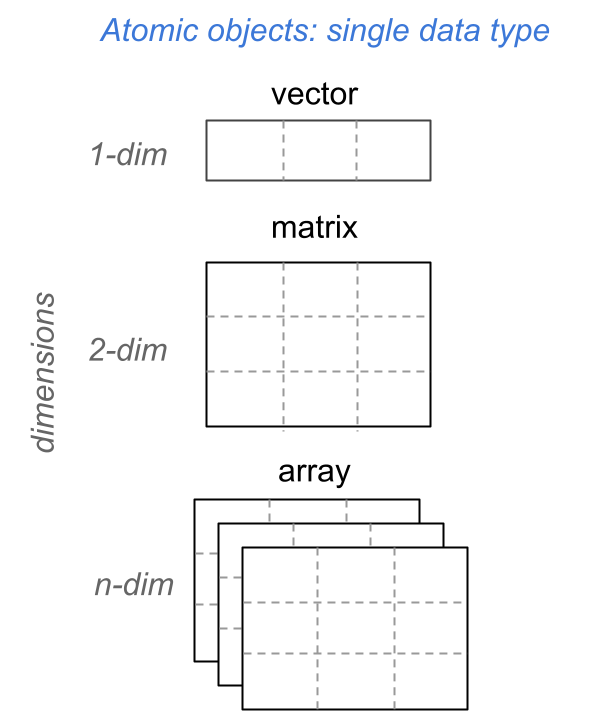
\includegraphics[width=0.5\linewidth]{images/objects/obj-atomics} 

}

\caption{Triad of atomic data objects in R.}\label{fig:unnamed-chunk-105}
\end{figure}

Personally, I prefer to reserve the term \texttt{array} for three or more dimensional
arrays. As you can tell from the above diagram, this is how I'm using this
term in the book. However, you should always keep in mind that a \texttt{matrix} is an
\texttt{array}. The other way around is not necessarily true: not all arrays are
matrices.

\hypertarget{creating-matrices-with-matrix}{%
\section{\texorpdfstring{Creating matrices with \texttt{matrix()}}{Creating matrices with matrix()}}\label{creating-matrices-with-matrix}}

The \texttt{cbind()} and \texttt{rbind()} functions provide a convenient way to create
matrices from different input vectors. But the kind of matrices that you can
create with them is limited if all you have is just one input vector.

So, in addition to \texttt{cbind()} and \texttt{rbind()}, R comes with the function \texttt{matrix()}
which is the workhorse function for creating matrices. Usually, you provide
an input vector, and also the number of rows and columns (i.e.~the
\emph{matrix dimensions}) that the returned matrix should have.

Here is how to use \texttt{matrix()} to create the \texttt{savings} matrix that we are
interested in obtaining:

\begin{Shaded}
\begin{Highlighting}[]
\NormalTok{savings }\OtherTok{=} \FunctionTok{matrix}\NormalTok{(}\FunctionTok{c}\NormalTok{(years, amounts), }\AttributeTok{nrow =} \DecValTok{6}\NormalTok{, }\AttributeTok{ncol =} \DecValTok{2}\NormalTok{)}
\NormalTok{savings}
\SpecialCharTok{\textgreater{}}\NormalTok{      [,}\DecValTok{1}\NormalTok{]     [,}\DecValTok{2}\NormalTok{]}
\SpecialCharTok{\textgreater{}}\NormalTok{ [}\DecValTok{1}\NormalTok{,]    }\DecValTok{0} \FloatTok{1000.000}
\SpecialCharTok{\textgreater{}}\NormalTok{ [}\DecValTok{2}\NormalTok{,]    }\DecValTok{1} \FloatTok{1020.000}
\SpecialCharTok{\textgreater{}}\NormalTok{ [}\DecValTok{3}\NormalTok{,]    }\DecValTok{2} \FloatTok{1040.400}
\SpecialCharTok{\textgreater{}}\NormalTok{ [}\DecValTok{4}\NormalTok{,]    }\DecValTok{3} \FloatTok{1061.208}
\SpecialCharTok{\textgreater{}}\NormalTok{ [}\DecValTok{5}\NormalTok{,]    }\DecValTok{4} \FloatTok{1082.432}
\SpecialCharTok{\textgreater{}}\NormalTok{ [}\DecValTok{6}\NormalTok{,]    }\DecValTok{5} \FloatTok{1104.081}
\end{Highlighting}
\end{Shaded}

This is an interesting piece of code. Notice that \texttt{years} and \texttt{amounts} are
combined into a single vector, which is the main input of \texttt{matrix()}. The two
other arguments correspond to the matrix dimensions: \texttt{nrow\ =\ 6} tells R that
we want to produce a matrix with 6 rows; \texttt{ncol\ =\ 2} indicates that we want the
matrix to have 2 columns.

\hypertarget{column-major-matrices}{%
\subsection{Column-Major Matrices}\label{column-major-matrices}}

When creating a matrix via the function \texttt{matrix()}, R takes into consideration
three important aspects:

\begin{enumerate}
\def\labelenumi{\arabic{enumi})}
\item
  the length of the input vector.
\item
  the ``size'' of the matrix given by its number of rows and columns; think of
  this as the total number of cells or entries in the matrix.
\item
  whether the length of the input vector is a multiple or sub-multiple of the
  size of the matrix.
\end{enumerate}

In the current example, the input vector \texttt{c(years,\ amounts)} has 12 elements.
In turn, the size of the desired matrix is given by the multiplication of the
number of rows (2) times the number of columns (6), that is:

\[
\text{size of matrix} = 6 \times 2 = 12 \text{ cells}
\]

R then compares the length of the input vector against the size of the matrix.
If these numbers are the same, like in this example, R proceeds to split the
elements of the input vector into 2 sections or sub-vectors, each one
containing 6 elements. Each of these sections will become a column of the
output matrix.

In other words, the vector \texttt{c(years,\ amounts)} is split into 2 sub-vectors:

\begin{verbatim}
# the first sub-vector is:
0  1  2  3  4  5

# the second sub-vector is:
1000.000  1020.000  1040.400  1061.208  1082.432  1104.081
\end{verbatim}

The first sub-vector, which corresponds to \texttt{years}, becomes the first column.
The second sub-vector, which corresponds to \texttt{amounts}, becomes the second
column. In technical terms we say that R matrices are stored
\textbf{column-major} because of the mechanism used by R to arrange the elements of
an input vector in order to create a matrix.

\hypertarget{mismatch-between-length-of-input-vector-and-size-of-matrix}{%
\subsubsection*{Mismatch between length of input vector and size of matrix}\label{mismatch-between-length-of-input-vector-and-size-of-matrix}}
\addcontentsline{toc}{subsubsection}{Mismatch between length of input vector and size of matrix}

What about those cases in which the length of the input vector does not match
the size of the desired matrix? For example, consider the following commands
illustrating this type of situation:

\begin{Shaded}
\begin{Highlighting}[]
\CommentTok{\# examples in which length of input vector}
\CommentTok{\# does not match size of matrix}
\NormalTok{m1 }\OtherTok{=} \FunctionTok{matrix}\NormalTok{(}\DecValTok{1}\SpecialCharTok{:}\DecValTok{3}\NormalTok{, }\AttributeTok{nrow =} \DecValTok{3}\NormalTok{, }\AttributeTok{ncol =} \DecValTok{2}\NormalTok{)}

\NormalTok{m2 }\OtherTok{=} \FunctionTok{matrix}\NormalTok{(}\DecValTok{1}\SpecialCharTok{:}\DecValTok{3}\NormalTok{, }\AttributeTok{nrow =} \DecValTok{2}\NormalTok{, }\AttributeTok{ncol =} \DecValTok{3}\NormalTok{)}

\NormalTok{m3 }\OtherTok{=} \FunctionTok{matrix}\NormalTok{(}\DecValTok{1}\SpecialCharTok{:}\DecValTok{12}\NormalTok{, }\AttributeTok{nrow =} \DecValTok{3}\NormalTok{, }\AttributeTok{ncol =} \DecValTok{2}\NormalTok{)}
\SpecialCharTok{\textgreater{}}\NormalTok{ Warning }\ControlFlowTok{in} \FunctionTok{matrix}\NormalTok{(}\DecValTok{1}\SpecialCharTok{:}\DecValTok{12}\NormalTok{, }\AttributeTok{nrow =} \DecValTok{3}\NormalTok{, }\AttributeTok{ncol =} \DecValTok{2}\NormalTok{)}\SpecialCharTok{:}\NormalTok{ data}
\SpecialCharTok{\textgreater{}}\NormalTok{ length differs from size of matrix}\SpecialCharTok{:}\NormalTok{ [}\DecValTok{12} \SpecialCharTok{!=} \DecValTok{3}\NormalTok{ x }\DecValTok{2}\NormalTok{]}

\NormalTok{m4 }\OtherTok{=} \FunctionTok{matrix}\NormalTok{(}\DecValTok{1}\SpecialCharTok{:}\DecValTok{4}\NormalTok{, }\AttributeTok{nrow =} \DecValTok{3}\NormalTok{, }\AttributeTok{ncol =} \DecValTok{2}\NormalTok{)}
\SpecialCharTok{\textgreater{}}\NormalTok{ Warning }\ControlFlowTok{in} \FunctionTok{matrix}\NormalTok{(}\DecValTok{1}\SpecialCharTok{:}\DecValTok{4}\NormalTok{, }\AttributeTok{nrow =} \DecValTok{3}\NormalTok{, }\AttributeTok{ncol =} \DecValTok{2}\NormalTok{)}\SpecialCharTok{:}\NormalTok{ data}
\SpecialCharTok{\textgreater{}}\NormalTok{ length [}\DecValTok{4}\NormalTok{] is not a sub}\SpecialCharTok{{-}}\NormalTok{multiple or multiple of}
\SpecialCharTok{\textgreater{}}\NormalTok{ the number of rows [}\DecValTok{3}\NormalTok{]}

\NormalTok{m5 }\OtherTok{=} \FunctionTok{matrix}\NormalTok{(}\DecValTok{1}\SpecialCharTok{:}\DecValTok{8}\NormalTok{, }\AttributeTok{nrow =} \DecValTok{2}\NormalTok{, }\AttributeTok{ncol =} \DecValTok{3}\NormalTok{)}
\SpecialCharTok{\textgreater{}}\NormalTok{ Warning }\ControlFlowTok{in} \FunctionTok{matrix}\NormalTok{(}\DecValTok{1}\SpecialCharTok{:}\DecValTok{8}\NormalTok{, }\AttributeTok{nrow =} \DecValTok{2}\NormalTok{, }\AttributeTok{ncol =} \DecValTok{3}\NormalTok{)}\SpecialCharTok{:}\NormalTok{ data}
\SpecialCharTok{\textgreater{}}\NormalTok{ length [}\DecValTok{8}\NormalTok{] is not a sub}\SpecialCharTok{{-}}\NormalTok{multiple or multiple of}
\SpecialCharTok{\textgreater{}}\NormalTok{ the number of columns [}\DecValTok{3}\NormalTok{]}
\end{Highlighting}
\end{Shaded}

In matrices \texttt{m1} and \texttt{m2} the input vector \texttt{1:3} is a sub-multiple of the size
of the matrix 6.

In matrix \texttt{m3} the input vector \texttt{1:12} is longer than the size of the matrix: 6.
However, the entire length of the vector, 12, is a multiple of the size 6.

In matrices \texttt{m4} and \texttt{m5}, all the input vectors have lengths that are
neither a multiple or sub-multiple of the size of the returned matrix.

When the length of the input vector does not match the size of the desired
matrix, R applies its recycling rules. Let's pay attention to \texttt{m1}:

\begin{Shaded}
\begin{Highlighting}[]
\NormalTok{m1}
\SpecialCharTok{\textgreater{}}\NormalTok{      [,}\DecValTok{1}\NormalTok{] [,}\DecValTok{2}\NormalTok{]}
\SpecialCharTok{\textgreater{}}\NormalTok{ [}\DecValTok{1}\NormalTok{,]    }\DecValTok{1}    \DecValTok{1}
\SpecialCharTok{\textgreater{}}\NormalTok{ [}\DecValTok{2}\NormalTok{,]    }\DecValTok{2}    \DecValTok{2}
\SpecialCharTok{\textgreater{}}\NormalTok{ [}\DecValTok{3}\NormalTok{,]    }\DecValTok{3}    \DecValTok{3}
\end{Highlighting}
\end{Shaded}

Note how the values of the input vector \texttt{1:3} are recycled to form the columns
of \texttt{m1}. The values appear in the first column, but they also appear in the
second column after being recycled.

In contrast, matrix \texttt{m3} does not use all the elements in the input vector
\texttt{1:12}. Instead, only the first six values are retained.

As for the matrices \texttt{m4} and \texttt{m5}, they all have an input vector whose
length is neither a multiple nor a sub-multiple of the size of the matrix.
In these cases R will also apply its recycling rules, but it will also display
a warning message letting us know that the length of the input vector is not a
multiple or sub-multiple of either the number of rows or the number of columns.

\hypertarget{giving-names-to-rows-and-columns}{%
\subsection{Giving names to rows and columns}\label{giving-names-to-rows-and-columns}}

Often, you may need to provide names for either the rows and/or the columns of
a matrix. R comes with the functions \texttt{rownames()} and \texttt{colnames()} that can be
used to assign names for the rows and columns, for example:

\begin{Shaded}
\begin{Highlighting}[]
\CommentTok{\# matrix of savings amounts}
\NormalTok{savings }\OtherTok{=} \FunctionTok{matrix}\NormalTok{(}\FunctionTok{c}\NormalTok{(years, amounts), }\AttributeTok{nrow =} \DecValTok{6}\NormalTok{, }\AttributeTok{ncol =} \DecValTok{2}\NormalTok{)}

\CommentTok{\# row and columns names}
\FunctionTok{rownames}\NormalTok{(savings) }\OtherTok{=} \DecValTok{1}\SpecialCharTok{:}\DecValTok{6}
\FunctionTok{colnames}\NormalTok{(savings) }\OtherTok{=} \FunctionTok{c}\NormalTok{(}\StringTok{"year"}\NormalTok{, }\StringTok{"amount"}\NormalTok{)}

\NormalTok{savings}
\SpecialCharTok{\textgreater{}}\NormalTok{   year   amount}
\SpecialCharTok{\textgreater{}} \DecValTok{1}    \DecValTok{0} \FloatTok{1000.000}
\SpecialCharTok{\textgreater{}} \DecValTok{2}    \DecValTok{1} \FloatTok{1020.000}
\SpecialCharTok{\textgreater{}} \DecValTok{3}    \DecValTok{2} \FloatTok{1040.400}
\SpecialCharTok{\textgreater{}} \DecValTok{4}    \DecValTok{3} \FloatTok{1061.208}
\SpecialCharTok{\textgreater{}} \DecValTok{5}    \DecValTok{4} \FloatTok{1082.432}
\SpecialCharTok{\textgreater{}} \DecValTok{6}    \DecValTok{5} \FloatTok{1104.081}
\end{Highlighting}
\end{Shaded}

\hypertarget{more-matrices}{%
\subsection{More Matrices}\label{more-matrices}}

Let's make things a bit more complex. Say you have the following investments:

\begin{itemize}
\item
  \$1000 in a \textbf{savings account} that pays 2\% annual return, during 4 years
\item
  \$2000 in a \textbf{money market} account that pays 2.5\% annual return, during
  2 years
\item
  \$5000 in a \textbf{certificate of deposit} that pays 3\% annual return, during
  3 years
\end{itemize}

In R, we can calculate the future values of each type of investment product:

\begin{Shaded}
\begin{Highlighting}[]
\CommentTok{\# savings account}
\NormalTok{savings }\OtherTok{=} \DecValTok{1000} \SpecialCharTok{*}\NormalTok{ (}\DecValTok{1} \SpecialCharTok{+} \FloatTok{0.02}\NormalTok{)}\SpecialCharTok{\^{}}\NormalTok{(}\DecValTok{0}\SpecialCharTok{:}\DecValTok{4}\NormalTok{)}
\NormalTok{savings}
\SpecialCharTok{\textgreater{}}\NormalTok{ [}\DecValTok{1}\NormalTok{] }\FloatTok{1000.000} \FloatTok{1020.000} \FloatTok{1040.400} \FloatTok{1061.208} \FloatTok{1082.432}
\end{Highlighting}
\end{Shaded}

\begin{Shaded}
\begin{Highlighting}[]
\CommentTok{\# money market}
\NormalTok{moneymkt }\OtherTok{=} \DecValTok{2000} \SpecialCharTok{*}\NormalTok{ (}\DecValTok{1} \SpecialCharTok{+} \FloatTok{0.025}\NormalTok{)}\SpecialCharTok{\^{}}\NormalTok{(}\DecValTok{0}\SpecialCharTok{:}\DecValTok{2}\NormalTok{)}
\NormalTok{moneymkt}
\SpecialCharTok{\textgreater{}}\NormalTok{ [}\DecValTok{1}\NormalTok{] }\FloatTok{2000.00} \FloatTok{2050.00} \FloatTok{2101.25}
\end{Highlighting}
\end{Shaded}

\begin{Shaded}
\begin{Highlighting}[]
\CommentTok{\# certificate of deposit}
\NormalTok{certificate }\OtherTok{=} \DecValTok{5000} \SpecialCharTok{*}\NormalTok{ (}\DecValTok{1} \SpecialCharTok{+} \FloatTok{0.03}\NormalTok{)}\SpecialCharTok{\^{}}\NormalTok{(}\DecValTok{0}\SpecialCharTok{:}\DecValTok{3}\NormalTok{)}
\NormalTok{certificate}
\SpecialCharTok{\textgreater{}}\NormalTok{ [}\DecValTok{1}\NormalTok{] }\FloatTok{5000.000} \FloatTok{5150.000} \FloatTok{5304.500} \FloatTok{5463.635}
\end{Highlighting}
\end{Shaded}

\hypertarget{separated-matrices}{%
\subsubsection*{Separated matrices}\label{separated-matrices}}
\addcontentsline{toc}{subsubsection}{Separated matrices}

We can create individual matrices for each type of account:

\begin{Shaded}
\begin{Highlighting}[]
\CommentTok{\# savings account}
\NormalTok{sav\_mat }\OtherTok{=} \FunctionTok{cbind}\NormalTok{(}\DecValTok{0}\SpecialCharTok{:}\DecValTok{4}\NormalTok{, savings)}
\end{Highlighting}
\end{Shaded}

\begin{Shaded}
\begin{Highlighting}[]
\CommentTok{\# money market}
\NormalTok{mm\_mat }\OtherTok{=} \FunctionTok{cbind}\NormalTok{(}\DecValTok{0}\SpecialCharTok{:}\DecValTok{2}\NormalTok{, moneymkt)}
\end{Highlighting}
\end{Shaded}

\begin{Shaded}
\begin{Highlighting}[]
\CommentTok{\# certificate of deposit}
\NormalTok{cd\_mat }\OtherTok{=} \FunctionTok{cbind}\NormalTok{(}\DecValTok{0}\SpecialCharTok{:}\DecValTok{3}\NormalTok{, certificate)}
\end{Highlighting}
\end{Shaded}

\hypertarget{single-matrix}{%
\subsubsection*{Single matrix}\label{single-matrix}}
\addcontentsline{toc}{subsubsection}{Single matrix}

Alternatively, we can stack everything into a single matrix:

\begin{Shaded}
\begin{Highlighting}[]
\FunctionTok{cbind}\NormalTok{(}\FunctionTok{c}\NormalTok{(}\DecValTok{0}\SpecialCharTok{:}\DecValTok{4}\NormalTok{, }\DecValTok{0}\SpecialCharTok{:}\DecValTok{2}\NormalTok{, }\DecValTok{0}\SpecialCharTok{:}\DecValTok{3}\NormalTok{), }\FunctionTok{c}\NormalTok{(savings, moneymkt, certificate))}
\SpecialCharTok{\textgreater{}}\NormalTok{       [,}\DecValTok{1}\NormalTok{]     [,}\DecValTok{2}\NormalTok{]}
\SpecialCharTok{\textgreater{}}\NormalTok{  [}\DecValTok{1}\NormalTok{,]    }\DecValTok{0} \FloatTok{1000.000}
\SpecialCharTok{\textgreater{}}\NormalTok{  [}\DecValTok{2}\NormalTok{,]    }\DecValTok{1} \FloatTok{1020.000}
\SpecialCharTok{\textgreater{}}\NormalTok{  [}\DecValTok{3}\NormalTok{,]    }\DecValTok{2} \FloatTok{1040.400}
\SpecialCharTok{\textgreater{}}\NormalTok{  [}\DecValTok{4}\NormalTok{,]    }\DecValTok{3} \FloatTok{1061.208}
\SpecialCharTok{\textgreater{}}\NormalTok{  [}\DecValTok{5}\NormalTok{,]    }\DecValTok{4} \FloatTok{1082.432}
\SpecialCharTok{\textgreater{}}\NormalTok{  [}\DecValTok{6}\NormalTok{,]    }\DecValTok{0} \FloatTok{2000.000}
\SpecialCharTok{\textgreater{}}\NormalTok{  [}\DecValTok{7}\NormalTok{,]    }\DecValTok{1} \FloatTok{2050.000}
\SpecialCharTok{\textgreater{}}\NormalTok{  [}\DecValTok{8}\NormalTok{,]    }\DecValTok{2} \FloatTok{2101.250}
\SpecialCharTok{\textgreater{}}\NormalTok{  [}\DecValTok{9}\NormalTok{,]    }\DecValTok{0} \FloatTok{5000.000}
\SpecialCharTok{\textgreater{}}\NormalTok{ [}\DecValTok{10}\NormalTok{,]    }\DecValTok{1} \FloatTok{5150.000}
\SpecialCharTok{\textgreater{}}\NormalTok{ [}\DecValTok{11}\NormalTok{,]    }\DecValTok{2} \FloatTok{5304.500}
\SpecialCharTok{\textgreater{}}\NormalTok{ [}\DecValTok{12}\NormalTok{,]    }\DecValTok{3} \FloatTok{5463.635}
\end{Highlighting}
\end{Shaded}

\hypertarget{what-about-mixing-data-types}{%
\subsubsection*{What about mixing data types?}\label{what-about-mixing-data-types}}
\addcontentsline{toc}{subsubsection}{What about mixing data types?}

What if you want some table like this:

\begin{longtable}[]{@{}ccc@{}}
\toprule()
account & year & amount \\
\midrule()
\endhead
savings & 0 & 1000.000 \\
savings & 1 & 1020.000 \\
savings & 2 & 1040.400 \\
savings & 3 & 1061.208 \\
savings & 4 & 1082.432 \\
moneymkt & 0 & 2000.000 \\
moneymkt & 1 & 2050.000 \\
moneymkt & 2 & 2101.250 \\
certif & 0 & 5000.000 \\
certif & 1 & 5150.250 \\
certif & 2 & 5304.500 \\
certif & 3 & 5463.635 \\
\bottomrule()
\end{longtable}

We could use the \texttt{cbind()} function in an attempt to obtain a matrix having
a similar rectangular structure as in the above table:

\begin{Shaded}
\begin{Highlighting}[]
\NormalTok{investments }\OtherTok{=} \FunctionTok{cbind}\NormalTok{(}
  \FunctionTok{rep}\NormalTok{(}\FunctionTok{c}\NormalTok{(}\StringTok{"savings"}\NormalTok{, }\StringTok{"moneymkt"}\NormalTok{, }\StringTok{"certif"}\NormalTok{), }\AttributeTok{times =} \FunctionTok{c}\NormalTok{(}\DecValTok{5}\NormalTok{, }\DecValTok{3}\NormalTok{, }\DecValTok{4}\NormalTok{)),}
  \FunctionTok{c}\NormalTok{(}\DecValTok{0}\SpecialCharTok{:}\DecValTok{4}\NormalTok{, }\DecValTok{0}\SpecialCharTok{:}\DecValTok{2}\NormalTok{, }\DecValTok{0}\SpecialCharTok{:}\DecValTok{3}\NormalTok{), }
  \FunctionTok{c}\NormalTok{(savings, moneymkt, certificate))}

\NormalTok{investments}
\SpecialCharTok{\textgreater{}}\NormalTok{       [,}\DecValTok{1}\NormalTok{]       [,}\DecValTok{2}\NormalTok{] [,}\DecValTok{3}\NormalTok{]        }
\SpecialCharTok{\textgreater{}}\NormalTok{  [}\DecValTok{1}\NormalTok{,] }\StringTok{"savings"}  \StringTok{"0"}  \StringTok{"1000"}      
\SpecialCharTok{\textgreater{}}\NormalTok{  [}\DecValTok{2}\NormalTok{,] }\StringTok{"savings"}  \StringTok{"1"}  \StringTok{"1020"}      
\SpecialCharTok{\textgreater{}}\NormalTok{  [}\DecValTok{3}\NormalTok{,] }\StringTok{"savings"}  \StringTok{"2"}  \StringTok{"1040.4"}    
\SpecialCharTok{\textgreater{}}\NormalTok{  [}\DecValTok{4}\NormalTok{,] }\StringTok{"savings"}  \StringTok{"3"}  \StringTok{"1061.208"}  
\SpecialCharTok{\textgreater{}}\NormalTok{  [}\DecValTok{5}\NormalTok{,] }\StringTok{"savings"}  \StringTok{"4"}  \StringTok{"1082.43216"}
\SpecialCharTok{\textgreater{}}\NormalTok{  [}\DecValTok{6}\NormalTok{,] }\StringTok{"moneymkt"} \StringTok{"0"}  \StringTok{"2000"}      
\SpecialCharTok{\textgreater{}}\NormalTok{  [}\DecValTok{7}\NormalTok{,] }\StringTok{"moneymkt"} \StringTok{"1"}  \StringTok{"2050"}      
\SpecialCharTok{\textgreater{}}\NormalTok{  [}\DecValTok{8}\NormalTok{,] }\StringTok{"moneymkt"} \StringTok{"2"}  \StringTok{"2101.25"}   
\SpecialCharTok{\textgreater{}}\NormalTok{  [}\DecValTok{9}\NormalTok{,] }\StringTok{"certif"}   \StringTok{"0"}  \StringTok{"5000"}      
\SpecialCharTok{\textgreater{}}\NormalTok{ [}\DecValTok{10}\NormalTok{,] }\StringTok{"certif"}   \StringTok{"1"}  \StringTok{"5150"}      
\SpecialCharTok{\textgreater{}}\NormalTok{ [}\DecValTok{11}\NormalTok{,] }\StringTok{"certif"}   \StringTok{"2"}  \StringTok{"5304.5"}    
\SpecialCharTok{\textgreater{}}\NormalTok{ [}\DecValTok{12}\NormalTok{,] }\StringTok{"certif"}   \StringTok{"3"}  \StringTok{"5463.635"}
\end{Highlighting}
\end{Shaded}

Do you notice something funny with the matrix \texttt{investments}?

As you can tell, all the values in \texttt{investments} are displayed being surrounded
with double quotes. This indicates that all the values are of type \texttt{character}.
Why is this?

Recall that matrices are \textbf{atomic} objects. Usually, you provide an input
vector containing the elements to be arranged into a rectangular array with
a certain number of rows and columns. Because vectors are atomic, this property
is ``inherited'' by the returned matrix.

It turns out that you can use other classes of data objects, not necessarily
atomic, for creating a matrix. If the input object is non-atomic, R will
coerce it into a vector, making the input an atomic object.

So either way, whether you provide an atomic input or a non-atomic input,
to any of the matrix-creation functions, R will always produce an atomic
output. This is the reason why the below command produces a \texttt{character} matrix:

\begin{Shaded}
\begin{Highlighting}[]
\NormalTok{investments }\OtherTok{=} \FunctionTok{cbind}\NormalTok{(}
  \FunctionTok{rep}\NormalTok{(}\FunctionTok{c}\NormalTok{(}\StringTok{"savings"}\NormalTok{, }\StringTok{"moneymkt"}\NormalTok{, }\StringTok{"certif"}\NormalTok{), }\AttributeTok{times =} \FunctionTok{c}\NormalTok{(}\DecValTok{5}\NormalTok{, }\DecValTok{3}\NormalTok{, }\DecValTok{4}\NormalTok{)),}
  \FunctionTok{c}\NormalTok{(}\DecValTok{0}\SpecialCharTok{:}\DecValTok{4}\NormalTok{, }\DecValTok{0}\SpecialCharTok{:}\DecValTok{2}\NormalTok{, }\DecValTok{0}\SpecialCharTok{:}\DecValTok{3}\NormalTok{), }
  \FunctionTok{c}\NormalTok{(savings, moneymkt, certificate))}

\FunctionTok{typeof}\NormalTok{(investments)}
\SpecialCharTok{\textgreater{}}\NormalTok{ [}\DecValTok{1}\NormalTok{] }\StringTok{"character"}
\end{Highlighting}
\end{Shaded}

The three input vectors are coerced into a single vector of \texttt{character} data
type, causing the \texttt{investments} matrix to be of type \texttt{character}.

\begin{center}\rule{0.5\linewidth}{0.5pt}\end{center}

\hypertarget{exercises-4}{%
\section{Exercises}\label{exercises-4}}

\textbf{1)} Use \texttt{matrix()} to create a matrix \texttt{mat1} (see below) from the input
vector \texttt{x\ =\ letters{[}1:15{]}}:

\begin{verbatim}
# mat1
"a"  "d"  "g"  "j"  "m" 
"b"  "e"  "h"  "k"  "n" 
"c"  "f"  "i"  "l"  "o"
\end{verbatim}

\textbf{2)} Look at the documentation of \texttt{matrix()} and find how to use it for
obtaining the matrix \texttt{mat2} (see below) from the input vector \texttt{x\ =\ letters{[}1:15{]}}:

\begin{verbatim}
# mat2
"a"  "b"  "c"  "d"  "e" 
"f"  "g"  "h"  "i"  "j" 
"k"  "l"  "m"  "n"  "o" 
\end{verbatim}

\textbf{3)} Find out how to use the functions \texttt{rownames()} and \texttt{colnames()} to give
names to the rows and the columns of matrix \texttt{mat1}. Choose any names you want,
and display matrix \texttt{mat1}.

\textbf{4)} Use \texttt{matrix()} to create a matrix \texttt{mat3} (see below) from the input
vector \texttt{y\ =\ month.name}:

\begin{verbatim}
# mat3
"January" "February" "March"    
"April"   "May"      "June"     
"July"    "August"   "September"
"October" "November" "December" 
\end{verbatim}

\textbf{5)} Use \texttt{matrix()}---and its recycling principle---to create a matrix \texttt{mat4}
(see below) from the input vector \texttt{a\ =\ c(3,\ 6,\ 9)}:

\begin{verbatim}
# mat4
3    3    3
6    6    6
9    9    9
\end{verbatim}

\textbf{6)} Use \texttt{matrix()}---and its recycling principle---to create a matrix \texttt{mat5}
(see below) from the input vector \texttt{a\ =\ c(3,\ 6,\ 9)}:

\begin{verbatim}
# mat5
3    3    3
6    6    6
9    9    9
3    3    3
6    6    6
9    9    9
\end{verbatim}

\textbf{7)} Consider the following vectors \texttt{a} and \texttt{b}

\begin{Shaded}
\begin{Highlighting}[]
\NormalTok{a }\OtherTok{=} \FunctionTok{c}\NormalTok{(}\DecValTok{2}\NormalTok{, }\DecValTok{4}\NormalTok{, }\DecValTok{6}\NormalTok{)}
\NormalTok{b }\OtherTok{=} \FunctionTok{c}\NormalTok{(}\DecValTok{1}\NormalTok{, }\DecValTok{3}\NormalTok{, }\DecValTok{5}\NormalTok{)}
\end{Highlighting}
\end{Shaded}

Use the row-binding function \texttt{rbind()}, with inputs \texttt{a} and \texttt{b}, to create a
matrix \texttt{mat6} displayed below:

\begin{Shaded}
\begin{Highlighting}[]
\NormalTok{\# mat6}
\NormalTok{\textgreater{}      [,1] [,2] [,3]}
\NormalTok{\textgreater{} [1,]    1    3    5}
\NormalTok{\textgreater{} [2,]    2    4    6}
\end{Highlighting}
\end{Shaded}

\textbf{8)} Consider the following vectors \texttt{u} and \texttt{v}

\begin{Shaded}
\begin{Highlighting}[]
\NormalTok{u }\OtherTok{=} \FunctionTok{c}\NormalTok{(}\DecValTok{2}\NormalTok{, }\DecValTok{4}\NormalTok{, }\DecValTok{6}\NormalTok{, }\DecValTok{8}\NormalTok{)}
\NormalTok{v }\OtherTok{=} \FunctionTok{c}\NormalTok{(}\DecValTok{1}\NormalTok{, }\DecValTok{3}\NormalTok{, }\DecValTok{5}\NormalTok{, }\DecValTok{7}\NormalTok{)}
\end{Highlighting}
\end{Shaded}

Use the column-binding function \texttt{cbind()}, with inputs \texttt{u} and \texttt{v}, to create
a matrix \texttt{mat7} displayed below:

\begin{Shaded}
\begin{Highlighting}[]
\NormalTok{\# mat7}
\NormalTok{\textgreater{}      [,1] [,2] [,3]}
\NormalTok{\textgreater{} [1,]    2    1    2}
\NormalTok{\textgreater{} [2,]    4    3    4}
\NormalTok{\textgreater{} [3,]    6    5    6}
\NormalTok{\textgreater{} [4,]    8    7    8}
\end{Highlighting}
\end{Shaded}

\textbf{9)} Find out how to use the \texttt{diag()} function to create an \textbf{identity matrix}
of dimensions 4 rows and 4 columns (see below). BTW: An identity matrix is a
matrix with the same number of rows and columns, has ones in the diagonal,
and zeroes off-diagonal.

\begin{verbatim}
1    0    0    0
0    1    0    0
0    0    1    0
0    0    0    1
\end{verbatim}

\textbf{10)} Refer to matrices \texttt{mat4} and \texttt{mat7}. Use both \texttt{cbind()} and \texttt{rbind()}
to attempt binding these two matrices. If one of the binding operations fails,
explain why.

\hypertarget{matrices2}{%
\chapter{More About Matrices}\label{matrices2}}

Now that you have seen some ways to create matrices, let's discuss a number
of basic manipulations of matrices. I will show you examples of various
operations, and then you'll have the chance to put them in practice with some
exercises listed at the end of the chapter.

\hypertarget{basic-operations-with-matrices}{%
\section{Basic Operations with Matrices}\label{basic-operations-with-matrices}}

\begin{itemize}
\tightlist
\item
  Selecting elements:

  \begin{itemize}
  \tightlist
  \item
    select a given cell
  \item
    select a set of cells
  \item
    select a given row
  \item
    select a set of rows
  \item
    select a given column
  \item
    select a set of columns
  \end{itemize}
\item
  Adding a new column
\item
  Adding a new row
\item
  Deleting a column
\item
  Deleting a row
\item
  Renaming a column
\item
  Moving a column
\end{itemize}

Let's say you have a matrix \texttt{mat} with the following content:

\begin{Shaded}
\begin{Highlighting}[]
\CommentTok{\# inputs}
\NormalTok{deposit }\OtherTok{=} \DecValTok{1000}
\NormalTok{rate\_savings }\OtherTok{=} \FloatTok{0.02}
\NormalTok{rate\_moneymkt }\OtherTok{=} \FloatTok{0.025}
\NormalTok{rate\_certificate }\OtherTok{=} \FloatTok{0.03}
\NormalTok{years }\OtherTok{=} \DecValTok{0}\SpecialCharTok{:}\DecValTok{5}

\CommentTok{\# future values}
\NormalTok{savings }\OtherTok{=}\NormalTok{ deposit }\SpecialCharTok{*}\NormalTok{ (}\DecValTok{1} \SpecialCharTok{+}\NormalTok{ rate\_savings)}\SpecialCharTok{\^{}}\NormalTok{years}
\NormalTok{moneymkt }\OtherTok{=}\NormalTok{ deposit }\SpecialCharTok{*}\NormalTok{ (}\DecValTok{1} \SpecialCharTok{+}\NormalTok{ rate\_moneymkt)}\SpecialCharTok{\^{}}\NormalTok{years}
\NormalTok{certificate }\OtherTok{=}\NormalTok{ deposit }\SpecialCharTok{*}\NormalTok{ (}\DecValTok{1} \SpecialCharTok{+}\NormalTok{ rate\_certificate)}\SpecialCharTok{\^{}}\NormalTok{years}

\CommentTok{\# matrix}
\NormalTok{mat }\OtherTok{=} \FunctionTok{matrix}\NormalTok{(}\FunctionTok{c}\NormalTok{(years, savings, moneymkt, certificate), }\AttributeTok{nrow =} \DecValTok{6}\NormalTok{, }\AttributeTok{ncol =} \DecValTok{4}\NormalTok{)}

\CommentTok{\# row and columns names}
\FunctionTok{rownames}\NormalTok{(mat) }\OtherTok{=} \DecValTok{1}\SpecialCharTok{:}\DecValTok{6}
\FunctionTok{colnames}\NormalTok{(mat) }\OtherTok{=} \FunctionTok{c}\NormalTok{(}\StringTok{"year"}\NormalTok{, }\StringTok{"savings"}\NormalTok{, }\StringTok{"moneymkt"}\NormalTok{, }\StringTok{"certificate"}\NormalTok{)}

\NormalTok{mat}
\NormalTok{  year  savings moneymkt certificate}
\DecValTok{1}    \DecValTok{0} \FloatTok{1000.000} \FloatTok{1000.000}    \FloatTok{1000.000}
\DecValTok{2}    \DecValTok{1} \FloatTok{1020.000} \FloatTok{1025.000}    \FloatTok{1030.000}
\DecValTok{3}    \DecValTok{2} \FloatTok{1040.400} \FloatTok{1050.625}    \FloatTok{1060.900}
\DecValTok{4}    \DecValTok{3} \FloatTok{1061.208} \FloatTok{1076.891}    \FloatTok{1092.727}
\DecValTok{5}    \DecValTok{4} \FloatTok{1082.432} \FloatTok{1103.813}    \FloatTok{1125.509}
\DecValTok{6}    \DecValTok{5} \FloatTok{1104.081} \FloatTok{1131.408}    \FloatTok{1159.274}
\end{Highlighting}
\end{Shaded}

\hypertarget{selecting-elements}{%
\subsection{Selecting elements}\label{selecting-elements}}

The matrix \texttt{mat} is a 2-dimensional object: the 1st dimension corresponds
to the rows, while the 2nd dimension corresponds to the columns.
Because \texttt{mat} has two dimensions, the bracket notation involves
working with data frames in this form: \texttt{mat{[}\ ,\ {]}}.

\begin{figure}

{\centering 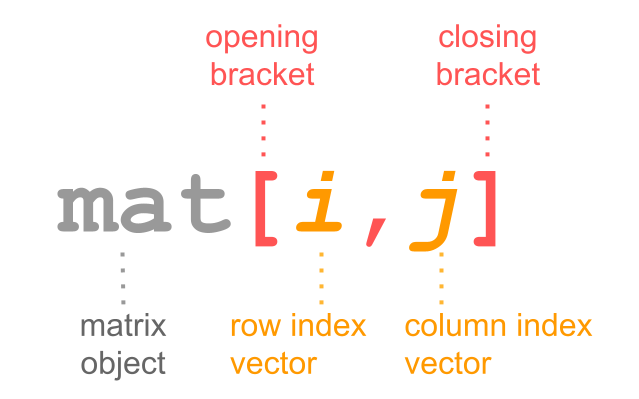
\includegraphics[width=0.5\linewidth]{images/objects/obj-matrix-brackets} 

}

\caption{Bracket notation in matrices}\label{fig:unnamed-chunk-125}
\end{figure}

In other words, you have to specify values inside the
brackets for the 1st index, and the 2nd index: \texttt{mat{[}index1,\ index2{]}}.

\hypertarget{selecting-cells}{%
\subsubsection*{Selecting cells}\label{selecting-cells}}
\addcontentsline{toc}{subsubsection}{Selecting cells}

\begin{figure}

{\centering 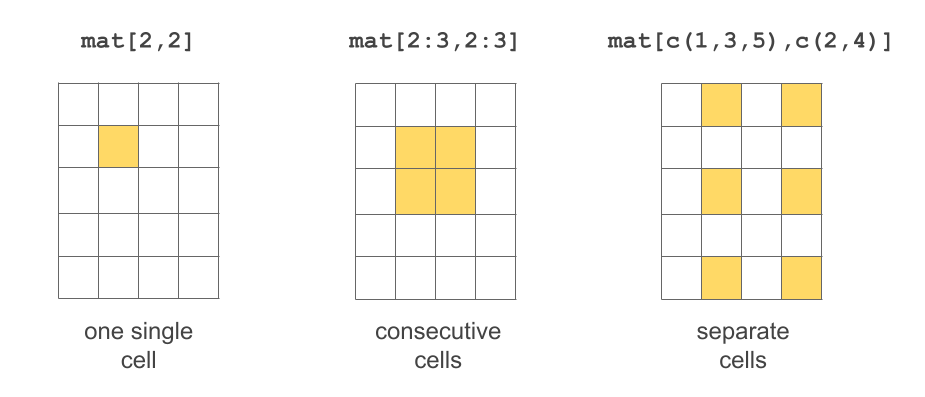
\includegraphics[width=0.8\linewidth]{images/objects/obj-matrix-cells1} 

}

\caption{Several ways to select cells}\label{fig:unnamed-chunk-126}
\end{figure}

\begin{Shaded}
\begin{Highlighting}[]
\CommentTok{\# select value in row 1 and column 1}
\NormalTok{mat[}\DecValTok{1}\NormalTok{, }\DecValTok{1}\NormalTok{]}
\SpecialCharTok{\textgreater{}}\NormalTok{ [}\DecValTok{1}\NormalTok{] }\DecValTok{0}

\CommentTok{\# select value in row 2 and column 3}
\NormalTok{mat[}\DecValTok{2}\NormalTok{, }\DecValTok{3}\NormalTok{]}
\SpecialCharTok{\textgreater{}}\NormalTok{ [}\DecValTok{1}\NormalTok{] }\DecValTok{1025}

\CommentTok{\# select values in these cells}
\NormalTok{mat[}\DecValTok{1}\SpecialCharTok{:}\DecValTok{2}\NormalTok{, }\DecValTok{3}\SpecialCharTok{:}\DecValTok{4}\NormalTok{]}
\SpecialCharTok{\textgreater{}}\NormalTok{   moneymkt certificate}
\SpecialCharTok{\textgreater{}} \DecValTok{1}     \DecValTok{1000}        \DecValTok{1000}
\SpecialCharTok{\textgreater{}} \DecValTok{2}     \DecValTok{1025}        \DecValTok{1030}
\end{Highlighting}
\end{Shaded}

It is also possible to exclude certain rows-and-columns by passing negative
numeric indices:

\begin{figure}

{\centering 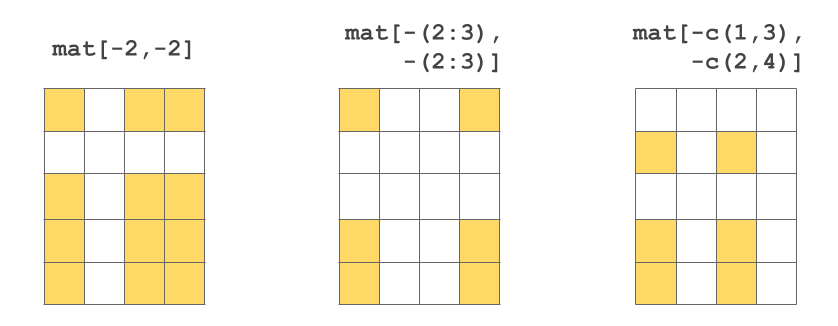
\includegraphics[width=0.8\linewidth]{images/objects/obj-matrix-cells2} 

}

\caption{Several ways to exclude cells}\label{fig:unnamed-chunk-128}
\end{figure}

\hypertarget{selecting-rows}{%
\subsubsection*{Selecting rows}\label{selecting-rows}}
\addcontentsline{toc}{subsubsection}{Selecting rows}

\begin{figure}

{\centering 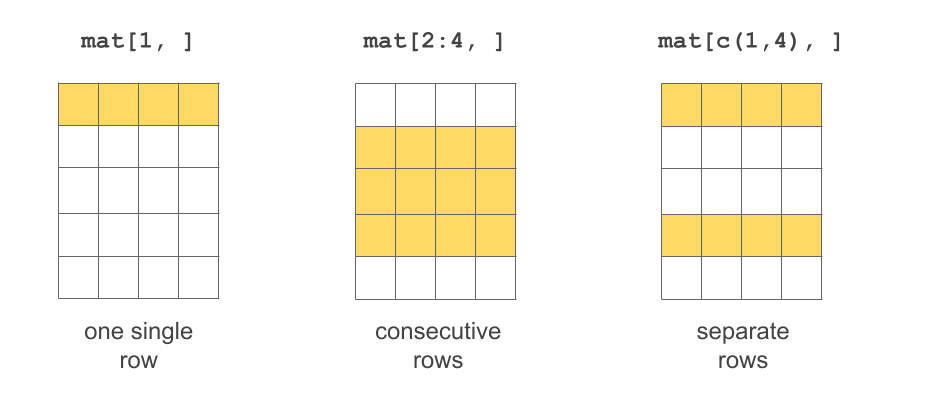
\includegraphics[width=0.8\linewidth]{images/objects/obj-matrix-rows1} 

}

\caption{Several ways to select rows}\label{fig:unnamed-chunk-129}
\end{figure}

If no value is specified for \texttt{index1} then all rows are included. Likewise,
if no value is specified for \texttt{index2} then all columns are included.

\begin{Shaded}
\begin{Highlighting}[]
\CommentTok{\# selecting first row}
\NormalTok{mat[}\DecValTok{1}\NormalTok{, ]}
\SpecialCharTok{\textgreater{}}\NormalTok{        year     savings    moneymkt certificate }
\SpecialCharTok{\textgreater{}}           \DecValTok{0}        \DecValTok{1000}        \DecValTok{1000}        \DecValTok{1000}

\CommentTok{\# selecting third row}
\NormalTok{mat[}\DecValTok{3}\NormalTok{, ]}
\SpecialCharTok{\textgreater{}}\NormalTok{        year     savings    moneymkt certificate }
\SpecialCharTok{\textgreater{}}       \FloatTok{2.000}    \FloatTok{1040.400}    \FloatTok{1050.625}    \FloatTok{1060.900}
\end{Highlighting}
\end{Shaded}

\begin{figure}

{\centering 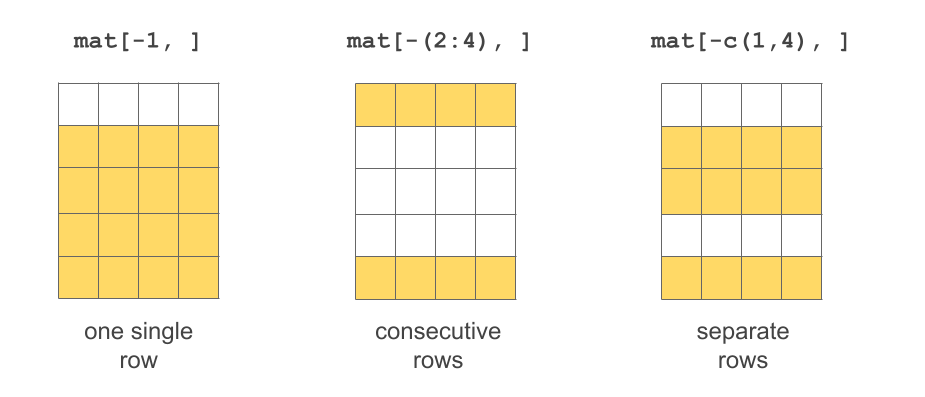
\includegraphics[width=0.8\linewidth]{images/objects/obj-matrix-rows2} 

}

\caption{Several ways to exclude rows}\label{fig:unnamed-chunk-131}
\end{figure}

\hypertarget{selecting-columns}{%
\subsubsection*{Selecting columns}\label{selecting-columns}}
\addcontentsline{toc}{subsubsection}{Selecting columns}

\begin{figure}

{\centering 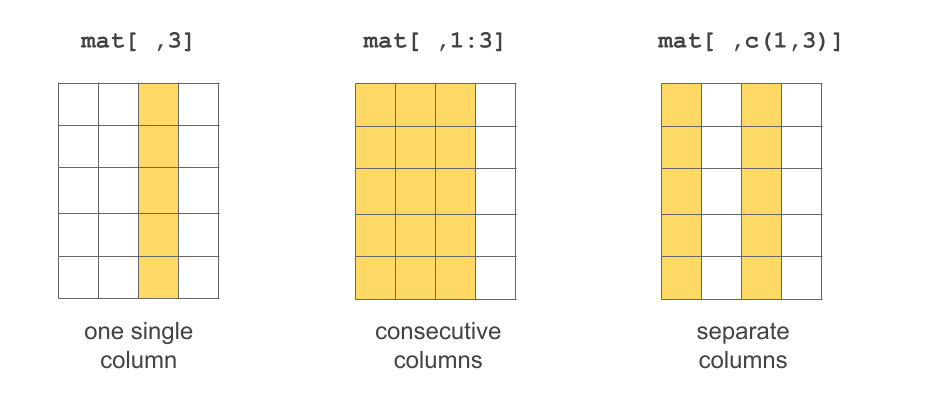
\includegraphics[width=0.8\linewidth]{images/objects/obj-matrix-cols1} 

}

\caption{Several ways to select columns}\label{fig:unnamed-chunk-132}
\end{figure}

\begin{Shaded}
\begin{Highlighting}[]
\CommentTok{\# selecting second column}
\NormalTok{mat[ ,}\DecValTok{2}\NormalTok{]}
\SpecialCharTok{\textgreater{}}        \DecValTok{1}        \DecValTok{2}        \DecValTok{3}        \DecValTok{4}        \DecValTok{5} 
\SpecialCharTok{\textgreater{}} \FloatTok{1000.000} \FloatTok{1020.000} \FloatTok{1040.400} \FloatTok{1061.208} \FloatTok{1082.432} 
\SpecialCharTok{\textgreater{}}        \DecValTok{6} 
\SpecialCharTok{\textgreater{}} \FloatTok{1104.081}

\CommentTok{\# selecting columns 2 to 4}
\NormalTok{mat[ ,}\DecValTok{2}\SpecialCharTok{:}\DecValTok{4}\NormalTok{]}
\SpecialCharTok{\textgreater{}}\NormalTok{    savings moneymkt certificate}
\SpecialCharTok{\textgreater{}} \DecValTok{1} \FloatTok{1000.000} \FloatTok{1000.000}    \FloatTok{1000.000}
\SpecialCharTok{\textgreater{}} \DecValTok{2} \FloatTok{1020.000} \FloatTok{1025.000}    \FloatTok{1030.000}
\SpecialCharTok{\textgreater{}} \DecValTok{3} \FloatTok{1040.400} \FloatTok{1050.625}    \FloatTok{1060.900}
\SpecialCharTok{\textgreater{}} \DecValTok{4} \FloatTok{1061.208} \FloatTok{1076.891}    \FloatTok{1092.727}
\SpecialCharTok{\textgreater{}} \DecValTok{5} \FloatTok{1082.432} \FloatTok{1103.813}    \FloatTok{1125.509}
\SpecialCharTok{\textgreater{}} \DecValTok{6} \FloatTok{1104.081} \FloatTok{1131.408}    \FloatTok{1159.274}
\end{Highlighting}
\end{Shaded}

\begin{figure}

{\centering 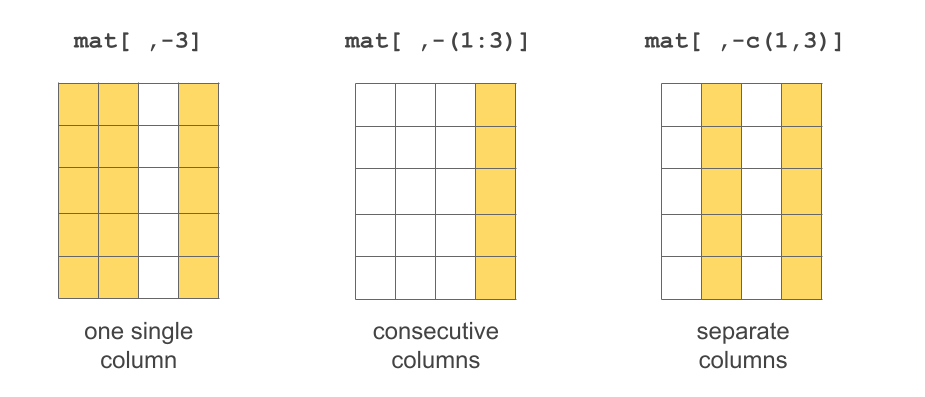
\includegraphics[width=0.8\linewidth]{images/objects/obj-matrix-cols2} 

}

\caption{Several ways to exclude columns}\label{fig:unnamed-chunk-134}
\end{figure}

\hypertarget{adding-a-column}{%
\subsection{Adding a column}\label{adding-a-column}}

To add a column, use the column-bind function \texttt{cbind()}

\begin{Shaded}
\begin{Highlighting}[]
\CommentTok{\# vector}
\NormalTok{vec }\OtherTok{\textless{}{-}} \FunctionTok{c}\NormalTok{(}\DecValTok{2}\NormalTok{, }\DecValTok{4}\NormalTok{, }\DecValTok{6}\NormalTok{, }\DecValTok{8}\NormalTok{, }\DecValTok{10}\NormalTok{, }\DecValTok{12}\NormalTok{)}

\CommentTok{\# adding weights to mat}
\NormalTok{mat }\OtherTok{\textless{}{-}} \FunctionTok{cbind}\NormalTok{(mat, vec)}
\NormalTok{mat}
\SpecialCharTok{\textgreater{}}\NormalTok{   year  savings moneymkt certificate vec}
\SpecialCharTok{\textgreater{}} \DecValTok{1}    \DecValTok{0} \FloatTok{1000.000} \FloatTok{1000.000}    \FloatTok{1000.000}   \DecValTok{2}
\SpecialCharTok{\textgreater{}} \DecValTok{2}    \DecValTok{1} \FloatTok{1020.000} \FloatTok{1025.000}    \FloatTok{1030.000}   \DecValTok{4}
\SpecialCharTok{\textgreater{}} \DecValTok{3}    \DecValTok{2} \FloatTok{1040.400} \FloatTok{1050.625}    \FloatTok{1060.900}   \DecValTok{6}
\SpecialCharTok{\textgreater{}} \DecValTok{4}    \DecValTok{3} \FloatTok{1061.208} \FloatTok{1076.891}    \FloatTok{1092.727}   \DecValTok{8}
\SpecialCharTok{\textgreater{}} \DecValTok{5}    \DecValTok{4} \FloatTok{1082.432} \FloatTok{1103.813}    \FloatTok{1125.509}  \DecValTok{10}
\SpecialCharTok{\textgreater{}} \DecValTok{6}    \DecValTok{5} \FloatTok{1104.081} \FloatTok{1131.408}    \FloatTok{1159.274}  \DecValTok{12}
\end{Highlighting}
\end{Shaded}

\hypertarget{deleting-a-column}{%
\subsection{Deleting a column}\label{deleting-a-column}}

What if you want to delete a column? Simple: use a negative index to exclude
the undesired column(s)

\begin{Shaded}
\begin{Highlighting}[]
\CommentTok{\# deleting fifth column}
\NormalTok{mat }\OtherTok{\textless{}{-}}\NormalTok{ mat[ ,}\SpecialCharTok{{-}}\DecValTok{5}\NormalTok{]}
\NormalTok{mat}
\SpecialCharTok{\textgreater{}}\NormalTok{   year  savings moneymkt certificate}
\SpecialCharTok{\textgreater{}} \DecValTok{1}    \DecValTok{0} \FloatTok{1000.000} \FloatTok{1000.000}    \FloatTok{1000.000}
\SpecialCharTok{\textgreater{}} \DecValTok{2}    \DecValTok{1} \FloatTok{1020.000} \FloatTok{1025.000}    \FloatTok{1030.000}
\SpecialCharTok{\textgreater{}} \DecValTok{3}    \DecValTok{2} \FloatTok{1040.400} \FloatTok{1050.625}    \FloatTok{1060.900}
\SpecialCharTok{\textgreater{}} \DecValTok{4}    \DecValTok{3} \FloatTok{1061.208} \FloatTok{1076.891}    \FloatTok{1092.727}
\SpecialCharTok{\textgreater{}} \DecValTok{5}    \DecValTok{4} \FloatTok{1082.432} \FloatTok{1103.813}    \FloatTok{1125.509}
\SpecialCharTok{\textgreater{}} \DecValTok{6}    \DecValTok{5} \FloatTok{1104.081} \FloatTok{1131.408}    \FloatTok{1159.274}
\end{Highlighting}
\end{Shaded}

\hypertarget{moving-a-column}{%
\subsection{Moving a column}\label{moving-a-column}}

What if you want to move one or more columns to a different position? For
example, what if you want to move \texttt{year} to the last position (last column)?
One option is to create a vector of column indices in the desired order, and then
use this vector (for the index of columns) to reassign the matrix like this:

\begin{Shaded}
\begin{Highlighting}[]
\NormalTok{reordered\_cols }\OtherTok{\textless{}{-}} \FunctionTok{c}\NormalTok{(}\DecValTok{2}\SpecialCharTok{:}\DecValTok{4}\NormalTok{, }\DecValTok{1}\NormalTok{)}
\NormalTok{mat }\OtherTok{\textless{}{-}}\NormalTok{ mat[ ,reordered\_cols]}
\NormalTok{mat}
\SpecialCharTok{\textgreater{}}\NormalTok{    savings moneymkt certificate year}
\SpecialCharTok{\textgreater{}} \DecValTok{1} \FloatTok{1000.000} \FloatTok{1000.000}    \FloatTok{1000.000}    \DecValTok{0}
\SpecialCharTok{\textgreater{}} \DecValTok{2} \FloatTok{1020.000} \FloatTok{1025.000}    \FloatTok{1030.000}    \DecValTok{1}
\SpecialCharTok{\textgreater{}} \DecValTok{3} \FloatTok{1040.400} \FloatTok{1050.625}    \FloatTok{1060.900}    \DecValTok{2}
\SpecialCharTok{\textgreater{}} \DecValTok{4} \FloatTok{1061.208} \FloatTok{1076.891}    \FloatTok{1092.727}    \DecValTok{3}
\SpecialCharTok{\textgreater{}} \DecValTok{5} \FloatTok{1082.432} \FloatTok{1103.813}    \FloatTok{1125.509}    \DecValTok{4}
\SpecialCharTok{\textgreater{}} \DecValTok{6} \FloatTok{1104.081} \FloatTok{1131.408}    \FloatTok{1159.274}    \DecValTok{5}
\end{Highlighting}
\end{Shaded}

\hypertarget{part-non-atomic-objects}{%
\part{Non-Atomic Objects}\label{part-non-atomic-objects}}

\hypertarget{lists}{%
\chapter{Lists}\label{lists}}

In this chapter, you will learn about R lists, the most generic type of data
container in R. Here's a summary of the main features of R lists:

\begin{itemize}
\tightlist
\item
  Lists are the most general class of data container
\item
  Like vectors, lists group data into a one-dimensional set
\item
  Unlike vectors, lists can store all kinds of objects
\item
  Lists can be of any length
\item
  Elements of a list can be named, or not
\end{itemize}

\hypertarget{motivation-2}{%
\section{Motivation}\label{motivation-2}}

In the chapter about \protect\hyperlink{matrices1}{Matrices and Arrays} we considered a small
portfolio consisting of the following three investments:

\begin{enumerate}
\def\labelenumi{\alph{enumi})}
\item
  \$1000 in a \textbf{savings account} that pays 2\% annual return, during 4 years
\item
  \$2000 in a \textbf{money market} account that pays 2.5\% annual return, during
  2 years
\item
  \$5000 in a \textbf{certificate of deposit} that pays 3\% annual return, during
  3 years
\end{enumerate}

Let's pay attention to the first investment: the savings account. Suppose I'm
interested in creating an object to store the specifications of this investment,
that is, I would like to have an R object with four elements

\begin{itemize}
\tightlist
\item
  the initial deposit: \texttt{1000}
\item
  the annual rate of return: \texttt{0.02}
\item
  the number of years: \texttt{4L}
\item
  and the type of account: \texttt{"savings"}
\end{itemize}

What kind of object could I use? With all the things we've discussed so far,
a natural decision would be to store these values in a vector:

\begin{Shaded}
\begin{Highlighting}[]
\NormalTok{investment1\_specs }\OtherTok{=} \FunctionTok{c}\NormalTok{(}
  \StringTok{"deposit"} \OtherTok{=} \DecValTok{1000}\NormalTok{,      }\CommentTok{\# double}
  \StringTok{"rate"} \OtherTok{=} \FloatTok{0.02}\NormalTok{,         }\CommentTok{\# double}
  \StringTok{"years"} \OtherTok{=}\NormalTok{ 4L,          }\CommentTok{\# integer}
  \StringTok{"account"} \OtherTok{=} \StringTok{"savings"}  \CommentTok{\# character}
\NormalTok{)}
\end{Highlighting}
\end{Shaded}

Notice that I'm creating \texttt{investment1\_specs} by mixing elements of different
data types: a couple of double types, an integer type, and a character type.
Thus, a very pertinent question is: What kind of vector is \texttt{investment1\_specs}?
If your answer to the preceding question was \emph{character}, then congrats!
By now, I expect that you can correctly answer this question without any
trouble. If that is not the case then go back to chapter
\protect\hyperlink{vectors3}{Creating Vectors} and reread the section on \protect\hyperlink{coercion}{Coercion}.

One simple way to confirm that \texttt{investment1\_specs} is indeed of \texttt{"character"}
type is by simply inspecting its contents:

\begin{Shaded}
\begin{Highlighting}[]
\NormalTok{investment1\_specs}
\SpecialCharTok{\textgreater{}}\NormalTok{   deposit      rate     years   account }
\SpecialCharTok{\textgreater{}}    \StringTok{"1000"}    \StringTok{"0.02"}       \StringTok{"4"} \StringTok{"savings"}
\end{Highlighting}
\end{Shaded}

While the \texttt{investment1\_specs} object ``technically'' is storing the specifications
of the savings account, all the initial numeric values have been coerced into
characters, which may not be the best way to store this information. The
solution to this limitation that vectors and other atomic objects have is to
employ another kind of object in R: \textbf{lists}.

\hypertarget{lists-1}{%
\section{Lists}\label{lists-1}}

An R list is the most generic kind of data object in R in the sense that
you can combine elements of different data types without them being coerced.

The primary function to create lists is the homonym function \texttt{list()}. To give
you an example of a basic list let us again pay attention to the specifications
of the first investment

\begin{itemize}
\tightlist
\item
  the initial deposit: \texttt{1000}
\item
  the annual rate of return: \texttt{0.02}
\item
  the number of years: \texttt{4L}
\item
  and the type of account: \texttt{"savings"}
\end{itemize}

Instead of using a vector, we can create a list to store these values. All we
have to do is use \texttt{list()} instead of \texttt{c()}:

\begin{Shaded}
\begin{Highlighting}[]
\NormalTok{specs1 }\OtherTok{=} \FunctionTok{list}\NormalTok{(}
  \StringTok{"deposit"} \OtherTok{=} \DecValTok{1000}\NormalTok{,      }\CommentTok{\# double}
  \StringTok{"rate"} \OtherTok{=} \FloatTok{0.02}\NormalTok{,         }\CommentTok{\# double}
  \StringTok{"years"} \OtherTok{=}\NormalTok{ 4L,          }\CommentTok{\# integer}
  \StringTok{"account"} \OtherTok{=} \StringTok{"savings"}  \CommentTok{\# character}
\NormalTok{)}

\NormalTok{specs1}
\SpecialCharTok{\textgreater{}} \ErrorTok{$}\NormalTok{deposit}
\SpecialCharTok{\textgreater{}}\NormalTok{ [}\DecValTok{1}\NormalTok{] }\DecValTok{1000}
\SpecialCharTok{\textgreater{}} 
\ErrorTok{\textgreater{}} \ErrorTok{$}\NormalTok{rate}
\SpecialCharTok{\textgreater{}}\NormalTok{ [}\DecValTok{1}\NormalTok{] }\FloatTok{0.02}
\SpecialCharTok{\textgreater{}} 
\ErrorTok{\textgreater{}} \ErrorTok{$}\NormalTok{years}
\SpecialCharTok{\textgreater{}}\NormalTok{ [}\DecValTok{1}\NormalTok{] }\DecValTok{4}
\SpecialCharTok{\textgreater{}} 
\ErrorTok{\textgreater{}} \ErrorTok{$}\NormalTok{account}
\SpecialCharTok{\textgreater{}}\NormalTok{ [}\DecValTok{1}\NormalTok{] }\StringTok{"savings"}
\end{Highlighting}
\end{Shaded}

Observe the way R prints a list with named elements. In contrast to the way
elements of a vector are displayed---in a contiguous form---the elements of a
list are displayed in a noncontiguous manner. Also, note how the names of the
elements are listed with a preappended dollar sign. For example, the first
element is \texttt{\$deposit}, the second element is \texttt{\$rate}, and so on.

What about the data type for each element of the list? From the visual inspection
of the elements in \texttt{specs1}, you can tell that all the numeric values are not
being coerced into strings. Which is what we were looking for. We were interested
in obtaining an object in which each of its elements gets to keep its data type.

If you try to use \texttt{typeof()} on a list in an attempt to get the data types of
its elements, I'm afraid this won't work the way you expect it:

\begin{Shaded}
\begin{Highlighting}[]
\FunctionTok{typeof}\NormalTok{(specs1)}
\SpecialCharTok{\textgreater{}}\NormalTok{ [}\DecValTok{1}\NormalTok{] }\StringTok{"list"}
\end{Highlighting}
\end{Shaded}

Applying \texttt{typeof()} on a list results in a not very interesting output \texttt{"list"}.

Getting ahead of myself momentarily, let me show you how to use the dollar
operator \texttt{\$} to refer to an named element of a list and check its data type:

\begin{Shaded}
\begin{Highlighting}[]
\FunctionTok{typeof}\NormalTok{(specs1}\SpecialCharTok{$}\NormalTok{deposit)}
\SpecialCharTok{\textgreater{}}\NormalTok{ [}\DecValTok{1}\NormalTok{] }\StringTok{"double"}

\FunctionTok{typeof}\NormalTok{(specs1}\SpecialCharTok{$}\NormalTok{account)}
\SpecialCharTok{\textgreater{}}\NormalTok{ [}\DecValTok{1}\NormalTok{] }\StringTok{"character"}
\end{Highlighting}
\end{Shaded}

We'll discuss the different ways in which you can subset elements of a list
later in this chapter.

\hypertarget{creating-lists}{%
\section{Creating Lists}\label{creating-lists}}

The typical way to create a list is with the function \texttt{list()}. This function
creates a list the same way \texttt{c()} creates a vector. Let's start with a simple
example creating three numeric vectors of same length, that we then use to
store them in a list:

\begin{Shaded}
\begin{Highlighting}[]
\NormalTok{vec1 }\OtherTok{\textless{}{-}} \DecValTok{1}\SpecialCharTok{:}\DecValTok{3}
\NormalTok{vec2 }\OtherTok{\textless{}{-}} \DecValTok{4}\SpecialCharTok{:}\DecValTok{6}
\NormalTok{vec3 }\OtherTok{\textless{}{-}} \DecValTok{7}\SpecialCharTok{:}\DecValTok{9}

\CommentTok{\# list with unnamed elements}
\NormalTok{lis }\OtherTok{\textless{}{-}} \FunctionTok{list}\NormalTok{(vec1, vec2, vec3)}
\NormalTok{lis}
\SpecialCharTok{\textgreater{}}\NormalTok{ [[}\DecValTok{1}\NormalTok{]]}
\SpecialCharTok{\textgreater{}}\NormalTok{ [}\DecValTok{1}\NormalTok{] }\DecValTok{1} \DecValTok{2} \DecValTok{3}
\SpecialCharTok{\textgreater{}} 
\ErrorTok{\textgreater{}}\NormalTok{ [[}\DecValTok{2}\NormalTok{]]}
\SpecialCharTok{\textgreater{}}\NormalTok{ [}\DecValTok{1}\NormalTok{] }\DecValTok{4} \DecValTok{5} \DecValTok{6}
\SpecialCharTok{\textgreater{}} 
\ErrorTok{\textgreater{}}\NormalTok{ [[}\DecValTok{3}\NormalTok{]]}
\SpecialCharTok{\textgreater{}}\NormalTok{ [}\DecValTok{1}\NormalTok{] }\DecValTok{7} \DecValTok{8} \DecValTok{9}
\end{Highlighting}
\end{Shaded}

Note how the contents of a list with unnamed elements are displayed: there is a
set of double brackets with an index indicating the position of each element,
and below each double bracket the corresponding vector is printed.

For illustration purposes, we could visualize the three input vectors and the
list with the following conceptual diagram.

\begin{figure}

{\centering 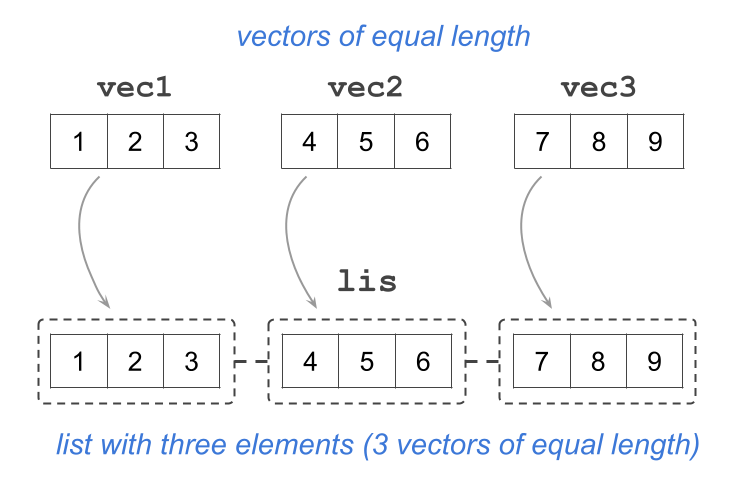
\includegraphics[width=0.6\linewidth]{images/objects/obj-list-vectors1} 

}

\caption{A list containing three unnamed elements (numeric vectors of length 3)}\label{fig:unnamed-chunk-145}
\end{figure}

Our intention with the depicted list as a set of discontinuous cells is to
convey the idea that a list is also a one-dimensional vector, albeit a very
special type of vector: a \textbf{non-atomic vector}. This means that each element
of a list can be any kind of object.

In the same way you can give names to elements of a vector, you can also give
names to elements of a list:

\begin{Shaded}
\begin{Highlighting}[]
\CommentTok{\# list with named elements}
\NormalTok{lis }\OtherTok{\textless{}{-}} \FunctionTok{list}\NormalTok{(}\StringTok{"vec1"} \OtherTok{=}\NormalTok{ vec1, }\StringTok{"vec2"} \OtherTok{=}\NormalTok{ vec2, }\StringTok{"vec3"} \OtherTok{=}\NormalTok{ vec3)}
\NormalTok{lis}
\SpecialCharTok{\textgreater{}} \ErrorTok{$}\NormalTok{vec1}
\SpecialCharTok{\textgreater{}}\NormalTok{ [}\DecValTok{1}\NormalTok{] }\DecValTok{1} \DecValTok{2} \DecValTok{3}
\SpecialCharTok{\textgreater{}} 
\ErrorTok{\textgreater{}} \ErrorTok{$}\NormalTok{vec2}
\SpecialCharTok{\textgreater{}}\NormalTok{ [}\DecValTok{1}\NormalTok{] }\DecValTok{4} \DecValTok{5} \DecValTok{6}
\SpecialCharTok{\textgreater{}} 
\ErrorTok{\textgreater{}} \ErrorTok{$}\NormalTok{vec3}
\SpecialCharTok{\textgreater{}}\NormalTok{ [}\DecValTok{1}\NormalTok{] }\DecValTok{7} \DecValTok{8} \DecValTok{9}
\end{Highlighting}
\end{Shaded}

When you create a list in this form, you can actually omit the quotes of
the given names. While this option of naming elements may create a bit of
confusion for beginners and inexperienced users in R, we believe it's not a big
deal (based on our experience):

\begin{Shaded}
\begin{Highlighting}[]
\CommentTok{\# another option for giving names to elements in a list}
\NormalTok{lis }\OtherTok{\textless{}{-}} \FunctionTok{list}\NormalTok{(}\AttributeTok{vec1 =}\NormalTok{ vec1, }\AttributeTok{vec2 =}\NormalTok{ vec2, }\AttributeTok{vec3 =}\NormalTok{ vec3)}
\NormalTok{lis}
\SpecialCharTok{\textgreater{}} \ErrorTok{$}\NormalTok{vec1}
\SpecialCharTok{\textgreater{}}\NormalTok{ [}\DecValTok{1}\NormalTok{] }\DecValTok{1} \DecValTok{2} \DecValTok{3}
\SpecialCharTok{\textgreater{}} 
\ErrorTok{\textgreater{}} \ErrorTok{$}\NormalTok{vec2}
\SpecialCharTok{\textgreater{}}\NormalTok{ [}\DecValTok{1}\NormalTok{] }\DecValTok{4} \DecValTok{5} \DecValTok{6}
\SpecialCharTok{\textgreater{}} 
\ErrorTok{\textgreater{}} \ErrorTok{$}\NormalTok{vec3}
\SpecialCharTok{\textgreater{}}\NormalTok{ [}\DecValTok{1}\NormalTok{] }\DecValTok{7} \DecValTok{8} \DecValTok{9}
\end{Highlighting}
\end{Shaded}

Observe how the contents of a list with named elements are displayed: this time,
instead of the set of double brackets, there is a dollar sign followed by the
name of the element, e.g.~\texttt{\$vec1}. Below each name, the corresponding vector is
printed.

The conceptual diagram in this case could look like this:

\begin{figure}

{\centering 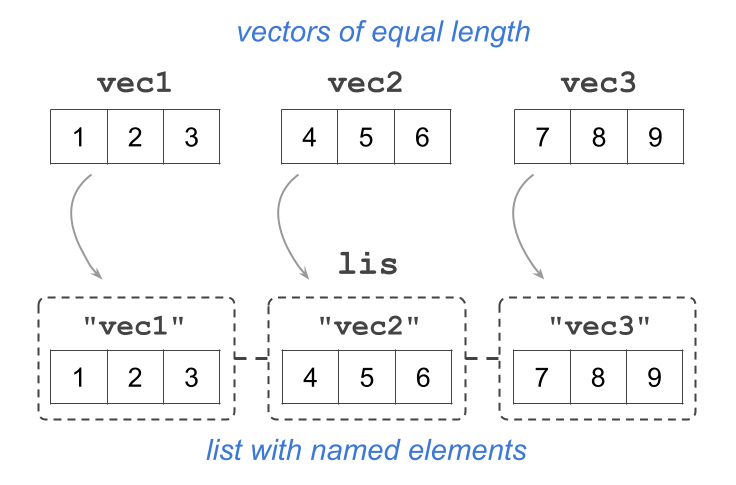
\includegraphics[width=0.6\linewidth]{images/objects/obj-list-vectors2} 

}

\caption{A list with named elements (numeric vectors of length 3)}\label{fig:unnamed-chunk-148}
\end{figure}

As we just said, the elements of a list can be any kind of R object. For
example, here's a list called \texttt{lst} that contains a character vector, a
numeric matrix, a factor, and another list:

\begin{Shaded}
\begin{Highlighting}[]
\NormalTok{lst }\OtherTok{\textless{}{-}} \FunctionTok{list}\NormalTok{(}
  \FunctionTok{c}\NormalTok{(}\StringTok{"savings"}\NormalTok{, }\StringTok{"money\_mkt"}\NormalTok{, }\StringTok{"certificate"}\NormalTok{),}
  \FunctionTok{matrix}\NormalTok{(}\DecValTok{1}\SpecialCharTok{:}\DecValTok{6}\NormalTok{, }\AttributeTok{nrow =} \DecValTok{2}\NormalTok{, }\AttributeTok{ncol =} \DecValTok{3}\NormalTok{),}
  \FunctionTok{factor}\NormalTok{(}\FunctionTok{c}\NormalTok{(}\StringTok{"yes"}\NormalTok{, }\StringTok{"no"}\NormalTok{, }\StringTok{"no"}\NormalTok{, }\StringTok{"no"}\NormalTok{, }\StringTok{"yes"}\NormalTok{)),}
  \FunctionTok{list}\NormalTok{(}\DecValTok{1000}\NormalTok{, }\DecValTok{2000}\NormalTok{, }\DecValTok{5000}\NormalTok{)}
\NormalTok{)}

\NormalTok{lst}
\SpecialCharTok{\textgreater{}}\NormalTok{ [[}\DecValTok{1}\NormalTok{]]}
\SpecialCharTok{\textgreater{}}\NormalTok{ [}\DecValTok{1}\NormalTok{] }\StringTok{"savings"}     \StringTok{"money\_mkt"}   \StringTok{"certificate"}
\SpecialCharTok{\textgreater{}} 
\ErrorTok{\textgreater{}}\NormalTok{ [[}\DecValTok{2}\NormalTok{]]}
\SpecialCharTok{\textgreater{}}\NormalTok{      [,}\DecValTok{1}\NormalTok{] [,}\DecValTok{2}\NormalTok{] [,}\DecValTok{3}\NormalTok{]}
\SpecialCharTok{\textgreater{}}\NormalTok{ [}\DecValTok{1}\NormalTok{,]    }\DecValTok{1}    \DecValTok{3}    \DecValTok{5}
\SpecialCharTok{\textgreater{}}\NormalTok{ [}\DecValTok{2}\NormalTok{,]    }\DecValTok{2}    \DecValTok{4}    \DecValTok{6}
\SpecialCharTok{\textgreater{}} 
\ErrorTok{\textgreater{}}\NormalTok{ [[}\DecValTok{3}\NormalTok{]]}
\SpecialCharTok{\textgreater{}}\NormalTok{ [}\DecValTok{1}\NormalTok{] yes no  no  no  yes}
\SpecialCharTok{\textgreater{}}\NormalTok{ Levels}\SpecialCharTok{:}\NormalTok{ no yes}
\SpecialCharTok{\textgreater{}} 
\ErrorTok{\textgreater{}}\NormalTok{ [[}\DecValTok{4}\NormalTok{]]}
\SpecialCharTok{\textgreater{}}\NormalTok{ [[}\DecValTok{4}\NormalTok{]][[}\DecValTok{1}\NormalTok{]]}
\SpecialCharTok{\textgreater{}}\NormalTok{ [}\DecValTok{1}\NormalTok{] }\DecValTok{1000}
\SpecialCharTok{\textgreater{}} 
\ErrorTok{\textgreater{}}\NormalTok{ [[}\DecValTok{4}\NormalTok{]][[}\DecValTok{2}\NormalTok{]]}
\SpecialCharTok{\textgreater{}}\NormalTok{ [}\DecValTok{1}\NormalTok{] }\DecValTok{2000}
\SpecialCharTok{\textgreater{}} 
\ErrorTok{\textgreater{}}\NormalTok{ [[}\DecValTok{4}\NormalTok{]][[}\DecValTok{3}\NormalTok{]]}
\SpecialCharTok{\textgreater{}}\NormalTok{ [}\DecValTok{1}\NormalTok{] }\DecValTok{5000}
\end{Highlighting}
\end{Shaded}

Whenever possible, I strongly recommend giving names to the elements of a list.
Not only this makes it easy to identify one element from the others, but it also
gives you more flexibility to rearrange the contents of the list without having
to worry about the exact order or position they occupy.

\begin{Shaded}
\begin{Highlighting}[]
\CommentTok{\# whenever possible, give names to elements in a list}
\NormalTok{lst }\OtherTok{\textless{}{-}} \FunctionTok{list}\NormalTok{(}
  \AttributeTok{first =} \FunctionTok{c}\NormalTok{(}\StringTok{"savings"}\NormalTok{, }\StringTok{"money\_mkt"}\NormalTok{, }\StringTok{"certificate"}\NormalTok{),}
  \AttributeTok{second =} \FunctionTok{matrix}\NormalTok{(}\DecValTok{1}\SpecialCharTok{:}\DecValTok{6}\NormalTok{, }\AttributeTok{nrow =} \DecValTok{2}\NormalTok{, }\AttributeTok{ncol =} \DecValTok{3}\NormalTok{),}
  \AttributeTok{third =} \FunctionTok{factor}\NormalTok{(}\FunctionTok{c}\NormalTok{(}\StringTok{"yes"}\NormalTok{, }\StringTok{"no"}\NormalTok{, }\StringTok{"no"}\NormalTok{, }\StringTok{"no"}\NormalTok{, }\StringTok{"yes"}\NormalTok{)),}
  \AttributeTok{fourth =} \FunctionTok{list}\NormalTok{(}\DecValTok{1000}\NormalTok{, }\DecValTok{2000}\NormalTok{, }\DecValTok{5000}\NormalTok{)}
\NormalTok{)}
\end{Highlighting}
\end{Shaded}

\hypertarget{manipulating-lists}{%
\section{Manipulating Lists}\label{manipulating-lists}}

To manipulate the elements of a list you can use bracket notation. Because a
list is a vector, you can use single brackets (e.g.~\texttt{lis{[}1{]}}) as well as
double brackets (e.g.~\texttt{lis{[}{[}1{]}{]}}).

\begin{figure}

{\centering 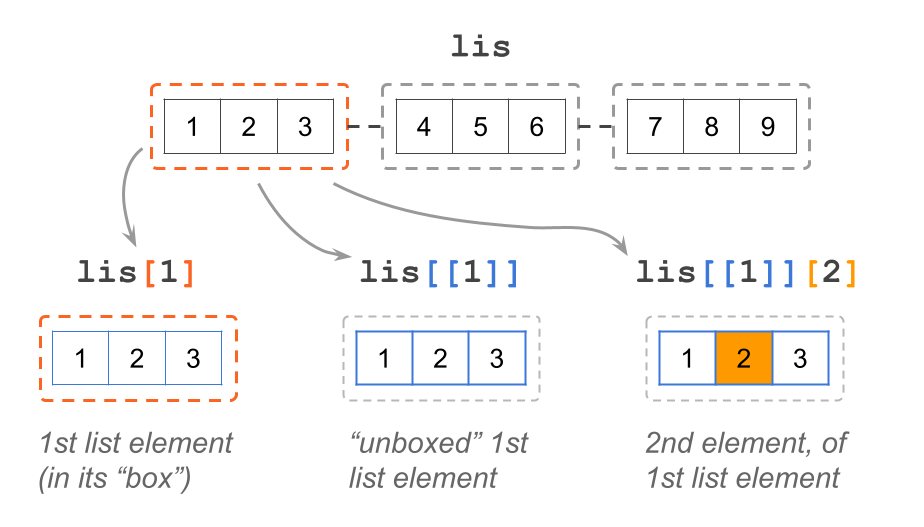
\includegraphics[width=0.75\linewidth]{images/objects/obj-list-brackets1} 

}

\caption{Bracket notation with lists}\label{fig:unnamed-chunk-151}
\end{figure}

\hypertarget{single-brackets}{%
\subsection{Single brackets}\label{single-brackets}}

Just like any other vector, and any other data object in R, you can use single
brackets on a list. For example, consider the unnamed version of a list, and
the use of single brackets with index \texttt{1} inside them:

\begin{Shaded}
\begin{Highlighting}[]
\CommentTok{\# list with unnamed elements}
\NormalTok{lis }\OtherTok{\textless{}{-}} \FunctionTok{list}\NormalTok{(vec1, vec2, vec3)}

\NormalTok{lis[}\DecValTok{1}\NormalTok{]}
\SpecialCharTok{\textgreater{}}\NormalTok{ [[}\DecValTok{1}\NormalTok{]]}
\SpecialCharTok{\textgreater{}}\NormalTok{ [}\DecValTok{1}\NormalTok{] }\DecValTok{1} \DecValTok{2} \DecValTok{3}
\end{Highlighting}
\end{Shaded}

What a single bracket does, is give you access to the ``container'' of the
specified element but without ``unboxing'' its contents. This is reflected by
the way in which the output is displayed: note the double bracket \texttt{{[}{[}1{]}{]}} in
the first line, and then \texttt{{[}1{]}\ 1\ 2\ 3} in the second line.

In other words, \texttt{lis{[}1{]}} gives you the first element of the list, which
contains a vector, but it does not give you direct access to the vector itself.
Put another way, \texttt{lis{[}1{]}} lets you see that the first element of the list is
a vector, but this vector is still \emph{inside} its ``box''.

\begin{figure}

{\centering 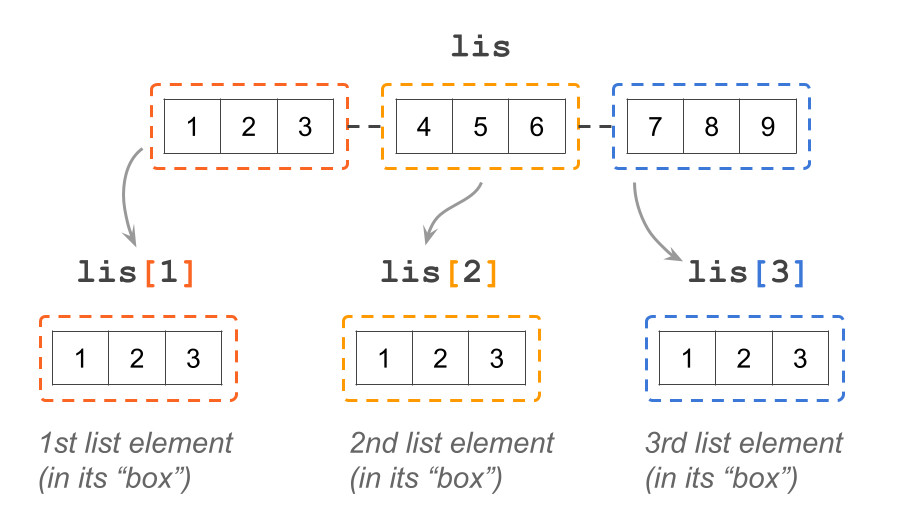
\includegraphics[width=0.75\linewidth]{images/objects/obj-list-brackets2} 

}

\caption{Use single brackets to select an element}\label{fig:unnamed-chunk-153}
\end{figure}

\hypertarget{double-brackets}{%
\subsection{Double Brackets}\label{double-brackets}}

In addition to single brackets, lists also accept double brackets: e.g.~
\texttt{lis{[}{[}1{]}{]}}

\begin{Shaded}
\begin{Highlighting}[]
\NormalTok{lis[[}\DecValTok{1}\NormalTok{]]}
\SpecialCharTok{\textgreater{}}\NormalTok{ [}\DecValTok{1}\NormalTok{] }\DecValTok{1} \DecValTok{2} \DecValTok{3}
\end{Highlighting}
\end{Shaded}

Double brackets are used when you want to get access to the content of the
list's elements. Notice the output of the previous command: now there are no
double brackets, just the output of the vector in the first position. Think
of this command as ``unboxing'' the object of the first element in \texttt{lis}.

What if you want to manipulate the elements of vector \texttt{vec1} or \texttt{vec2}? Use
double brackets followed by single brackets

\begin{Shaded}
\begin{Highlighting}[]
\CommentTok{\# second index of first list\textquotesingle{}s element}
\NormalTok{lis[[}\DecValTok{1}\NormalTok{]][}\DecValTok{2}\NormalTok{]}
\SpecialCharTok{\textgreater{}}\NormalTok{ [}\DecValTok{1}\NormalTok{] }\DecValTok{2}

\CommentTok{\# first index of second list\textquotesingle{}s element}
\NormalTok{lis[[}\DecValTok{2}\NormalTok{]][}\DecValTok{1}\NormalTok{]}
\SpecialCharTok{\textgreater{}}\NormalTok{ [}\DecValTok{1}\NormalTok{] }\DecValTok{4}
\end{Highlighting}
\end{Shaded}

\begin{figure}

{\centering 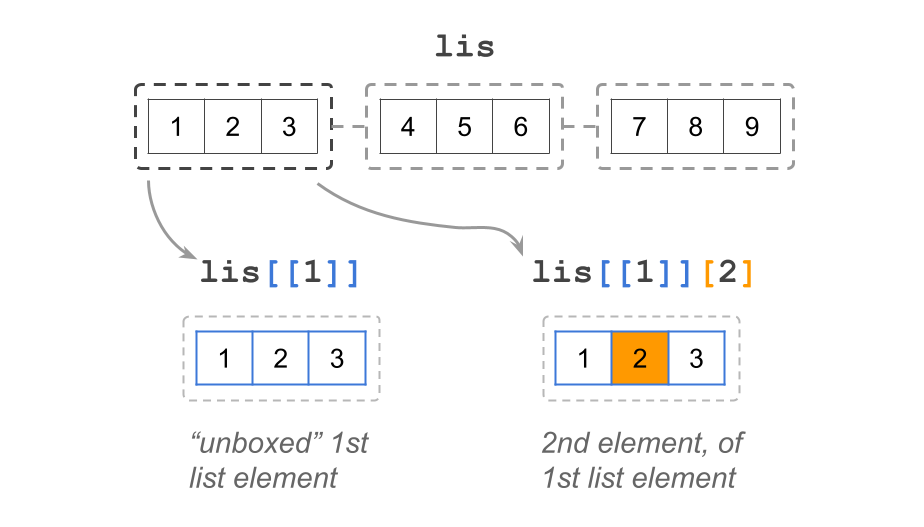
\includegraphics[width=0.75\linewidth]{images/objects/obj-list-brackets3} 

}

\caption{Use double brackets to extract an element}\label{fig:unnamed-chunk-156}
\end{figure}

\hypertarget{dollar-signs}{%
\subsection{Dollar signs}\label{dollar-signs}}

R lists---and data frames---follow an optional second system of notation for
extracting \textbf{named elements} using the dollar sign \textbf{\texttt{\$}}

\begin{figure}

{\centering 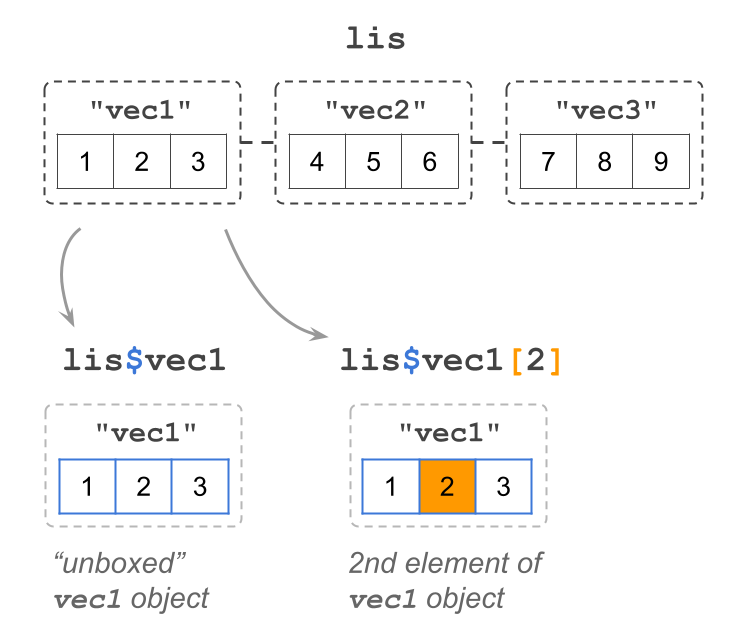
\includegraphics[width=0.6\linewidth]{images/objects/obj-list-dollars1} 

}

\caption{Dollar notation with lists}\label{fig:unnamed-chunk-157}
\end{figure}

Let's use the named version of \texttt{lis}:

\begin{Shaded}
\begin{Highlighting}[]
\CommentTok{\# list with named elements}
\NormalTok{lis }\OtherTok{\textless{}{-}} \FunctionTok{list}\NormalTok{(}\StringTok{"vec1"} \OtherTok{=}\NormalTok{ vec1, }\StringTok{"vec2"} \OtherTok{=}\NormalTok{ vec2, }\StringTok{"vec3"} \OtherTok{=}\NormalTok{ vec3)}

\NormalTok{lis}\SpecialCharTok{$}\NormalTok{vec1}
\SpecialCharTok{\textgreater{}}\NormalTok{ [}\DecValTok{1}\NormalTok{] }\DecValTok{1} \DecValTok{2} \DecValTok{3}
\end{Highlighting}
\end{Shaded}

The dollar sign \textbf{\texttt{\$}} notation works for selecting \textbf{named elements} in a
list. Notice the output of the above command: \texttt{lis\$vec1} gives you vector
\texttt{1\ 2\ 3}. In other words, dollar notation ``unboxes'' the object that is associated
to the specified name.

\hypertarget{adding-new-elements}{%
\subsection{Adding new elements}\label{adding-new-elements}}

From time to time, you will want to add one or more elements to an existing
list. For instance, consider a list \texttt{lst} with two elements:

\begin{Shaded}
\begin{Highlighting}[]
\NormalTok{lst }\OtherTok{\textless{}{-}} \FunctionTok{list}\NormalTok{(}\DecValTok{1}\SpecialCharTok{:}\DecValTok{3}\NormalTok{, }\FunctionTok{c}\NormalTok{(}\StringTok{\textquotesingle{}A\textquotesingle{}}\NormalTok{, }\StringTok{\textquotesingle{}B\textquotesingle{}}\NormalTok{, }\StringTok{\textquotesingle{}C\textquotesingle{}}\NormalTok{))}

\NormalTok{lst}
\SpecialCharTok{\textgreater{}}\NormalTok{ [[}\DecValTok{1}\NormalTok{]]}
\SpecialCharTok{\textgreater{}}\NormalTok{ [}\DecValTok{1}\NormalTok{] }\DecValTok{1} \DecValTok{2} \DecValTok{3}
\SpecialCharTok{\textgreater{}} 
\ErrorTok{\textgreater{}}\NormalTok{ [[}\DecValTok{2}\NormalTok{]]}
\SpecialCharTok{\textgreater{}}\NormalTok{ [}\DecValTok{1}\NormalTok{] }\StringTok{"A"} \StringTok{"B"} \StringTok{"C"}
\end{Highlighting}
\end{Shaded}

Say you want to add a logical vector as a third element to \texttt{lst}. One option to
do this is with double brackets, specifying a new index position to which you
assign the new element:

\begin{Shaded}
\begin{Highlighting}[]
\NormalTok{lst[[}\DecValTok{3}\NormalTok{]] }\OtherTok{\textless{}{-}} \FunctionTok{c}\NormalTok{(}\ConstantTok{TRUE}\NormalTok{, }\ConstantTok{FALSE}\NormalTok{, }\ConstantTok{TRUE}\NormalTok{, }\ConstantTok{FALSE}\NormalTok{)}

\NormalTok{lst}
\SpecialCharTok{\textgreater{}}\NormalTok{ [[}\DecValTok{1}\NormalTok{]]}
\SpecialCharTok{\textgreater{}}\NormalTok{ [}\DecValTok{1}\NormalTok{] }\DecValTok{1} \DecValTok{2} \DecValTok{3}
\SpecialCharTok{\textgreater{}} 
\ErrorTok{\textgreater{}}\NormalTok{ [[}\DecValTok{2}\NormalTok{]]}
\SpecialCharTok{\textgreater{}}\NormalTok{ [}\DecValTok{1}\NormalTok{] }\StringTok{"A"} \StringTok{"B"} \StringTok{"C"}
\SpecialCharTok{\textgreater{}} 
\ErrorTok{\textgreater{}}\NormalTok{ [[}\DecValTok{3}\NormalTok{]]}
\SpecialCharTok{\textgreater{}}\NormalTok{ [}\DecValTok{1}\NormalTok{]  }\ConstantTok{TRUE} \ConstantTok{FALSE}  \ConstantTok{TRUE} \ConstantTok{FALSE}
\end{Highlighting}
\end{Shaded}

Another option is to use the dollar operator by giving a new name to which you
assign the new element. Even though the previous elements in \texttt{lst}are unnamed,
the new added element will have an associated label:

\begin{Shaded}
\begin{Highlighting}[]
\NormalTok{lst}\SpecialCharTok{$}\NormalTok{new\_elem }\OtherTok{\textless{}{-}} \StringTok{\textquotesingle{}nuevo\textquotesingle{}}

\NormalTok{lst}
\SpecialCharTok{\textgreater{}}\NormalTok{ [[}\DecValTok{1}\NormalTok{]]}
\SpecialCharTok{\textgreater{}}\NormalTok{ [}\DecValTok{1}\NormalTok{] }\DecValTok{1} \DecValTok{2} \DecValTok{3}
\SpecialCharTok{\textgreater{}} 
\ErrorTok{\textgreater{}}\NormalTok{ [[}\DecValTok{2}\NormalTok{]]}
\SpecialCharTok{\textgreater{}}\NormalTok{ [}\DecValTok{1}\NormalTok{] }\StringTok{"A"} \StringTok{"B"} \StringTok{"C"}
\SpecialCharTok{\textgreater{}} 
\ErrorTok{\textgreater{}}\NormalTok{ [[}\DecValTok{3}\NormalTok{]]}
\SpecialCharTok{\textgreater{}}\NormalTok{ [}\DecValTok{1}\NormalTok{]  }\ConstantTok{TRUE} \ConstantTok{FALSE}  \ConstantTok{TRUE} \ConstantTok{FALSE}
\SpecialCharTok{\textgreater{}} 
\ErrorTok{\textgreater{}} \ErrorTok{$}\NormalTok{new\_elem}
\SpecialCharTok{\textgreater{}}\NormalTok{ [}\DecValTok{1}\NormalTok{] }\StringTok{"nuevo"}
\end{Highlighting}
\end{Shaded}

\hypertarget{removing-elements}{%
\subsection{Removing elements}\label{removing-elements}}

Just like you will want to add new elements in a list, you will also find
occasions in which you need to remove one or more elements. Take the previous
list \texttt{lst} with four elements, and say you want to remove the third element
(containing the logical vector)

\begin{Shaded}
\begin{Highlighting}[]
\NormalTok{lst}
\SpecialCharTok{\textgreater{}}\NormalTok{ [[}\DecValTok{1}\NormalTok{]]}
\SpecialCharTok{\textgreater{}}\NormalTok{ [}\DecValTok{1}\NormalTok{] }\DecValTok{1} \DecValTok{2} \DecValTok{3}
\SpecialCharTok{\textgreater{}} 
\ErrorTok{\textgreater{}}\NormalTok{ [[}\DecValTok{2}\NormalTok{]]}
\SpecialCharTok{\textgreater{}}\NormalTok{ [}\DecValTok{1}\NormalTok{] }\StringTok{"A"} \StringTok{"B"} \StringTok{"C"}
\SpecialCharTok{\textgreater{}} 
\ErrorTok{\textgreater{}}\NormalTok{ [[}\DecValTok{3}\NormalTok{]]}
\SpecialCharTok{\textgreater{}}\NormalTok{ [}\DecValTok{1}\NormalTok{]  }\ConstantTok{TRUE} \ConstantTok{FALSE}  \ConstantTok{TRUE} \ConstantTok{FALSE}
\SpecialCharTok{\textgreater{}} 
\ErrorTok{\textgreater{}} \ErrorTok{$}\NormalTok{new\_elem}
\SpecialCharTok{\textgreater{}}\NormalTok{ [}\DecValTok{1}\NormalTok{] }\StringTok{"nuevo"}
\end{Highlighting}
\end{Shaded}

To remove the third element, which is unnamed, you use double brackets and
assign a value \texttt{NULL} to that position:

\begin{Shaded}
\begin{Highlighting}[]
\NormalTok{lst[[}\DecValTok{3}\NormalTok{]] }\OtherTok{\textless{}{-}} \ConstantTok{NULL}
\NormalTok{lst}
\SpecialCharTok{\textgreater{}}\NormalTok{ [[}\DecValTok{1}\NormalTok{]]}
\SpecialCharTok{\textgreater{}}\NormalTok{ [}\DecValTok{1}\NormalTok{] }\DecValTok{1} \DecValTok{2} \DecValTok{3}
\SpecialCharTok{\textgreater{}} 
\ErrorTok{\textgreater{}}\NormalTok{ [[}\DecValTok{2}\NormalTok{]]}
\SpecialCharTok{\textgreater{}}\NormalTok{ [}\DecValTok{1}\NormalTok{] }\StringTok{"A"} \StringTok{"B"} \StringTok{"C"}
\SpecialCharTok{\textgreater{}} 
\ErrorTok{\textgreater{}} \ErrorTok{$}\NormalTok{new\_elem}
\SpecialCharTok{\textgreater{}}\NormalTok{ [}\DecValTok{1}\NormalTok{] }\StringTok{"nuevo"}
\end{Highlighting}
\end{Shaded}

As for those named elements, such as \texttt{lst\$new\_elem}, you do the same and assign
a \texttt{NULL} value, but this time using dollar notation:

\begin{Shaded}
\begin{Highlighting}[]
\NormalTok{lst}\SpecialCharTok{$}\NormalTok{new\_elem }\OtherTok{\textless{}{-}} \ConstantTok{NULL}
\NormalTok{lst}
\SpecialCharTok{\textgreater{}}\NormalTok{ [[}\DecValTok{1}\NormalTok{]]}
\SpecialCharTok{\textgreater{}}\NormalTok{ [}\DecValTok{1}\NormalTok{] }\DecValTok{1} \DecValTok{2} \DecValTok{3}
\SpecialCharTok{\textgreater{}} 
\ErrorTok{\textgreater{}}\NormalTok{ [[}\DecValTok{2}\NormalTok{]]}
\SpecialCharTok{\textgreater{}}\NormalTok{ [}\DecValTok{1}\NormalTok{] }\StringTok{"A"} \StringTok{"B"} \StringTok{"C"}
\end{Highlighting}
\end{Shaded}

\begin{center}\rule{0.5\linewidth}{0.5pt}\end{center}

\hypertarget{exercises-5}{%
\section{Exercises}\label{exercises-5}}

\textbf{1)} How would you create a list with your first name, middle name, and last
name? For example, something like:

\begin{verbatim}
$first
[1] "Gaston"

$middle
NULL

$last
[1] "Sanchez"
\end{verbatim}

\textbf{2)} Consider an R list \texttt{student} containing the following elements:

\begin{verbatim}
$name
[1] "Luke Skywalker"

$gpa
[1] 3.8

$major_minor
              major               minor 
     "jedi studies" "galactic policies" 

$grades
        course letter
1 light-sabers      B
2    force-101      A
3  jedi-poetry     C+
\end{verbatim}

\begin{enumerate}
\def\labelenumi{\alph{enumi})}
\tightlist
\item
  Which of the following commands gives you the values of column \texttt{letter}
  (i.e.~column of element \texttt{grades})? Mark all valid options.

  \begin{enumerate}
  \def\labelenumii{\roman{enumii})}
  \tightlist
  \item
    \texttt{student\$grades{[}\ ,letter{]}}
  \item
    \texttt{student\$grades{[}\ ,2{]}}
  \item
    \texttt{student{[}{[}4{]}{]}{[}\ ,2{]}}
  \item
    \texttt{student{[}4{]}{[}\ ,2{]}}
  \end{enumerate}
\item
  Which of the following commands gives you the length of \texttt{major\_minor}? Mark
  all valid options.

  \begin{enumerate}
  \def\labelenumii{\roman{enumii})}
  \tightlist
  \item
    \texttt{length(student{[}3{]})}
  \item
    \texttt{length(student\$major\_minor)}
  \item
    \texttt{length(student{[}c(FALSE,\ FALSE,\ TRUE,\ FALSE){]})}
  \item
    \texttt{length(student{[}{[}3{]}{]})}
  \end{enumerate}
\item
  Which of the following commands gives you the number of rows in \texttt{grades}?
  Mark all the valid options.

  \begin{enumerate}
  \def\labelenumii{\roman{enumii})}
  \tightlist
  \item
    \texttt{nrow(student{[}{[}"grades"{]}{]})}
  \item
    \texttt{nrow(student{[}4{]})}
  \item
    \texttt{nrow(student\$grades)}
  \item
    \texttt{nrow(student{[}\ ,c("course",\ "letter"){]})}
  \end{enumerate}
\item
  Which of the following commands gives you the value in \texttt{name}?
  Mark all the valid options.

  \begin{enumerate}
  \def\labelenumii{\roman{enumii})}
  \tightlist
  \item
    \texttt{student(1)}
  \item
    \texttt{student\$name}
  \item
    \texttt{student{[}{[}name{]}{]}}
  \item
    \texttt{student{[}{[}-c(1,2,3){]}{]}}
  \end{enumerate}
\end{enumerate}

\textbf{3)} I have created an R object called \texttt{obj}, which looks like this when
printed on the console:

\begin{verbatim}
$exams
midterm   final 
    100      90 
Levels: 90 100

$grades
midterm   final 
   "A+"    "A-" 

$hws
  topic points
1     x    151
2     y    154
3     z    159
\end{verbatim}

Indicate whether each of the following statements is True or False.

\begin{enumerate}
\def\labelenumi{\alph{enumi})}
\item
  length of \texttt{obj\$hws} is 3
\item
  data type of \texttt{obj\$exams} could be double (i.e.~real)
\item
  \texttt{obj\$grades} cannot be a factor
\item
  \texttt{obj\$hws} could be a data frame
\item
  \texttt{obj\$hws} could be a matrix
\item
  column \texttt{points} in \texttt{obj\$hws} could be a factor
\end{enumerate}

\textbf{4)} Consider an R list \texttt{apprentice} containing the following elements:

\begin{verbatim}
$name
[1] "Anakin Skywalker"

$gpa
[1] 4

$major_minor
             major1              major2 
     "jedi studies"      "sith studies" 
              minor 
"galactic policies" 

$grades
        course score
1    force-101   9.3
2    podracing  10.0
3 light-sabers   8.5
\end{verbatim}

Without running the commands in R, write down what will appear at the console
when such commands are executed:

\begin{enumerate}
\def\labelenumi{\alph{enumi})}
\item
  \texttt{length(apprentice\$major\_minor)}
\item
  \texttt{apprentice\$gpa\ \textless{}\ 2.5}
\item
  \texttt{names(apprentice\$major\_minor)}
\item
  \texttt{rep(apprentice\$grades{[}{[}2{]}{]}{[}2{]},\ apprentice\$gpa)}
\item
  \texttt{apprentice\$grades{[}order(apprentice\$grades\$score),\ {]}}
\end{enumerate}

\hypertarget{dataframes}{%
\chapter{Data Frames}\label{dataframes}}

The most common format/structure for a data set is a tabular format:
with rows and columns (like a spreadsheet). When your data is in this shape,
most of the time you will work with R \textbf{data frames} (or similar rectangular
structures like a \texttt{"matrix"}, \texttt{"table"}, \texttt{"tibble"}, etc).

Learning how to manipulate data frames is among the most important
\emph{data computing} skills in R.
Nowadays, there are two primary approaches for manipulating data frames. One
is what I call the ``traditional'' or ``classic'' approach which is what I present
in this chapter. The other is the ``tidy'' approach which you can think of as a
modern version based on the \emph{tidy data} framework mainly developed by
Hadley Wickham. We leave the discussion of this alternative approach for later.

To make the most of the content covered in the next sections, I am assuming
that you are familiar with the rest of data objects covered in the previous
chapters of part ``II Data Objects in R''.

\hypertarget{r-data-frames}{%
\section{R Data Frames}\label{r-data-frames}}

A data frame is a special type of R list. In most cases, a data frame is
internally stored as a list of vectors or factors, in which each vector
(or factor) corresponds to a column. This implies that columns in a data frame
are typically atomic structures: all elements in a given column are of the same
data type. However, since a data frame is a list, you
can technically have any kind of object as a column. In practice, though,
having data frames with columns that are not vectors or factors is something
that does not make much sense.

\begin{figure}

{\centering 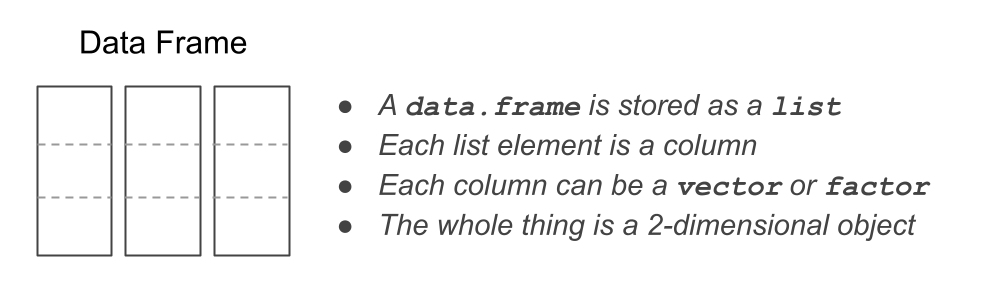
\includegraphics[width=0.75\linewidth]{images/objects/obj-dataframe} 

}

\caption{Abstract view of a data.frame}\label{fig:unnamed-chunk-170}
\end{figure}

From the data manipulation point of view, data frames behave like a hybrid
object. On one hand, they are lists and can be manipulated like any other list
using double brackets \texttt{dat{[}{[}\ {]}{]}} and dollar operator \texttt{dat\$name}.
On the other hand, because data frames are designed as tabular or 2-dimensional
objects, they also behave like two-dimensional arrays or matrices, admitting
bracket notation \texttt{dat{[}\ ,\ {]}}. For these reasons, there is a wide array of
functions that allows you to manipulate data frames in very convenient ways.
But to the inexperienced user, all these functions may feel overwhelming.

\hypertarget{inspecting-data-frames}{%
\section{Inspecting data frames}\label{inspecting-data-frames}}

One of the basic tasks when working with data frames involves inspecting its
contents. Specially in the early stages of data exploration, when dealing for
the first time with a new data frame, you will need to inspect things like
its overall structure, which includes its dimensions (number of rows and
columns), the data types of its columns, the names of columns and rows, and
also be able to take a peak to some of its first or last rows, and usually
obtain a summary of each column.

Let's see an example with one of the built-in data frames in R: \texttt{mtcars}.
Just a few rows and columns of \texttt{mtcars} are displayed below:

\begin{verbatim}
>                    mpg cyl disp  hp drat    wt
> Mazda RX4         21.0   6  160 110 3.90 2.620
> Mazda RX4 Wag     21.0   6  160 110 3.90 2.875
> Datsun 710        22.8   4  108  93 3.85 2.320
> Hornet 4 Drive    21.4   6  258 110 3.08 3.215
> Hornet Sportabout 18.7   8  360 175 3.15 3.440
\end{verbatim}

The main function to explore the \emph{structure} of not just a data frame, but of
any kind of object, is \texttt{str()}. When applied to data frames, \texttt{str()} returns a
report of the dimensions of the data frame, a list with the name of all the
variables, and their data types (e.g.~\texttt{chr} character, \texttt{num} real, etc).

\begin{Shaded}
\begin{Highlighting}[]
\FunctionTok{str}\NormalTok{(mtcars, }\AttributeTok{vec.len =} \DecValTok{1}\NormalTok{)}
\SpecialCharTok{\textgreater{}} \StringTok{\textquotesingle{}data.frame\textquotesingle{}}\SpecialCharTok{:} \DecValTok{32}\NormalTok{ obs. of  }\DecValTok{11}\NormalTok{ variables}\SpecialCharTok{:}
\ErrorTok{\textgreater{}}  \ErrorTok{$}\NormalTok{ mpg }\SpecialCharTok{:}\NormalTok{ num  }\DecValTok{21} \DecValTok{21}\NormalTok{ ...}
\SpecialCharTok{\textgreater{}}  \ErrorTok{$}\NormalTok{ cyl }\SpecialCharTok{:}\NormalTok{ num  }\DecValTok{6} \DecValTok{6}\NormalTok{ ...}
\SpecialCharTok{\textgreater{}}  \ErrorTok{$}\NormalTok{ disp}\SpecialCharTok{:}\NormalTok{ num  }\DecValTok{160} \DecValTok{160}\NormalTok{ ...}
\SpecialCharTok{\textgreater{}}  \ErrorTok{$}\NormalTok{ hp  }\SpecialCharTok{:}\NormalTok{ num  }\DecValTok{110} \DecValTok{110}\NormalTok{ ...}
\SpecialCharTok{\textgreater{}}  \ErrorTok{$}\NormalTok{ drat}\SpecialCharTok{:}\NormalTok{ num  }\FloatTok{3.9} \FloatTok{3.9}\NormalTok{ ...}
\SpecialCharTok{\textgreater{}}  \ErrorTok{$}\NormalTok{ wt  }\SpecialCharTok{:}\NormalTok{ num  }\FloatTok{2.62}\NormalTok{ ...}
\SpecialCharTok{\textgreater{}}  \ErrorTok{$}\NormalTok{ qsec}\SpecialCharTok{:}\NormalTok{ num  }\FloatTok{16.5}\NormalTok{ ...}
\SpecialCharTok{\textgreater{}}  \ErrorTok{$}\NormalTok{ vs  }\SpecialCharTok{:}\NormalTok{ num  }\DecValTok{0} \DecValTok{0}\NormalTok{ ...}
\SpecialCharTok{\textgreater{}}  \ErrorTok{$}\NormalTok{ am  }\SpecialCharTok{:}\NormalTok{ num  }\DecValTok{1} \DecValTok{1}\NormalTok{ ...}
\SpecialCharTok{\textgreater{}}  \ErrorTok{$}\NormalTok{ gear}\SpecialCharTok{:}\NormalTok{ num  }\DecValTok{4} \DecValTok{4}\NormalTok{ ...}
\SpecialCharTok{\textgreater{}}  \ErrorTok{$}\NormalTok{ carb}\SpecialCharTok{:}\NormalTok{ num  }\DecValTok{4} \DecValTok{4}\NormalTok{ ...}
\end{Highlighting}
\end{Shaded}

The argument \texttt{vec.len\ =\ 1} is optional but we like to use it because it
indicates that just the first elements in each column should be displayed.
Observe the output returned by \texttt{str()}. The first line tells us that \texttt{mtcars}
is an object of class \texttt{\textquotesingle{}data.frame\textquotesingle{}} with 32 observations (rows) and 11 variables
(columns). Then, the set of 11 variables is listed below, each line starting
with the dollar \texttt{\$} operator, followed by the name of the variable, followed
by a colon \texttt{:}, the data mode (all numeric \texttt{num} variables in this case),
and then a couple of values in each variable.

It is specially useful to check the data type of each column in order to catch
potential issues and avoid disastrous consequences or bugs in subsequent stages.

Here's a list of useful functions to inspect a data frame:

\begin{itemize}
\tightlist
\item
  \texttt{str()}: overall structure
\item
  \texttt{head()}: first rows
\item
  \texttt{tail()}: last rows
\item
  \texttt{summary()}: descriptive statistics
\item
  \texttt{dim()}: dimensions
\item
  \texttt{nrow()}: number of rows
\item
  \texttt{ncol()}: number of columns
\item
  \texttt{names()}: names of list elements (i.e.~column names)
\item
  \texttt{colnames()}: column names
\item
  \texttt{rownames()}: row names
\item
  \texttt{dimnames()}: list with column and row names
\end{itemize}

On a technical side, we should mention that a data frame is a list with special
attributes: an attribute \texttt{names} for column names, an attribute
\texttt{row.names} for row names, and of course its attribute \texttt{class}:

\begin{Shaded}
\begin{Highlighting}[]
\FunctionTok{attributes}\NormalTok{(mtcars)}
\SpecialCharTok{\textgreater{}} \ErrorTok{$}\NormalTok{names}
\SpecialCharTok{\textgreater{}}\NormalTok{  [}\DecValTok{1}\NormalTok{] }\StringTok{"mpg"}  \StringTok{"cyl"}  \StringTok{"disp"} \StringTok{"hp"}   \StringTok{"drat"} \StringTok{"wt"}  
\SpecialCharTok{\textgreater{}}\NormalTok{  [}\DecValTok{7}\NormalTok{] }\StringTok{"qsec"} \StringTok{"vs"}   \StringTok{"am"}   \StringTok{"gear"} \StringTok{"carb"}
\SpecialCharTok{\textgreater{}} 
\ErrorTok{\textgreater{}} \ErrorTok{$}\NormalTok{row.names}
\SpecialCharTok{\textgreater{}}\NormalTok{  [}\DecValTok{1}\NormalTok{] }\StringTok{"Mazda RX4"}           \StringTok{"Mazda RX4 Wag"}      
\SpecialCharTok{\textgreater{}}\NormalTok{  [}\DecValTok{3}\NormalTok{] }\StringTok{"Datsun 710"}          \StringTok{"Hornet 4 Drive"}     
\SpecialCharTok{\textgreater{}}\NormalTok{  [}\DecValTok{5}\NormalTok{] }\StringTok{"Hornet Sportabout"}   \StringTok{"Valiant"}            
\SpecialCharTok{\textgreater{}}\NormalTok{  [}\DecValTok{7}\NormalTok{] }\StringTok{"Duster 360"}          \StringTok{"Merc 240D"}          
\SpecialCharTok{\textgreater{}}\NormalTok{  [}\DecValTok{9}\NormalTok{] }\StringTok{"Merc 230"}            \StringTok{"Merc 280"}           
\SpecialCharTok{\textgreater{}}\NormalTok{ [}\DecValTok{11}\NormalTok{] }\StringTok{"Merc 280C"}           \StringTok{"Merc 450SE"}         
\SpecialCharTok{\textgreater{}}\NormalTok{ [}\DecValTok{13}\NormalTok{] }\StringTok{"Merc 450SL"}          \StringTok{"Merc 450SLC"}        
\SpecialCharTok{\textgreater{}}\NormalTok{ [}\DecValTok{15}\NormalTok{] }\StringTok{"Cadillac Fleetwood"}  \StringTok{"Lincoln Continental"}
\SpecialCharTok{\textgreater{}}\NormalTok{ [}\DecValTok{17}\NormalTok{] }\StringTok{"Chrysler Imperial"}   \StringTok{"Fiat 128"}           
\SpecialCharTok{\textgreater{}}\NormalTok{ [}\DecValTok{19}\NormalTok{] }\StringTok{"Honda Civic"}         \StringTok{"Toyota Corolla"}     
\SpecialCharTok{\textgreater{}}\NormalTok{ [}\DecValTok{21}\NormalTok{] }\StringTok{"Toyota Corona"}       \StringTok{"Dodge Challenger"}   
\SpecialCharTok{\textgreater{}}\NormalTok{ [}\DecValTok{23}\NormalTok{] }\StringTok{"AMC Javelin"}         \StringTok{"Camaro Z28"}         
\SpecialCharTok{\textgreater{}}\NormalTok{ [}\DecValTok{25}\NormalTok{] }\StringTok{"Pontiac Firebird"}    \StringTok{"Fiat X1{-}9"}          
\SpecialCharTok{\textgreater{}}\NormalTok{ [}\DecValTok{27}\NormalTok{] }\StringTok{"Porsche 914{-}2"}       \StringTok{"Lotus Europa"}       
\SpecialCharTok{\textgreater{}}\NormalTok{ [}\DecValTok{29}\NormalTok{] }\StringTok{"Ford Pantera L"}      \StringTok{"Ferrari Dino"}       
\SpecialCharTok{\textgreater{}}\NormalTok{ [}\DecValTok{31}\NormalTok{] }\StringTok{"Maserati Bora"}       \StringTok{"Volvo 142E"}         
\SpecialCharTok{\textgreater{}} 
\ErrorTok{\textgreater{}} \ErrorTok{$}\NormalTok{class}
\SpecialCharTok{\textgreater{}}\NormalTok{ [}\DecValTok{1}\NormalTok{] }\StringTok{"data.frame"}
\end{Highlighting}
\end{Shaded}

\hypertarget{creating-data-frames}{%
\section{Creating data frames}\label{creating-data-frames}}

Most of the (raw) data tables you will be working with will already be in
some data file. However, from time to time you will face the need to create
some sort of data table in R. In these situations, you will likely have to
create such table with a data frame. So let's look at various ways to
``manually'''' create a data frame.

\textbf{Option 1}: The primary option to build a data frame is with \texttt{data.frame()}.
You pass a series of vectors (or factors), of the same length, separated by commas.
Each vector (or factor) will become a column in the generated data frame.
Preferably, give names to each column like in the example below:

\begin{Shaded}
\begin{Highlighting}[]
\NormalTok{dat }\OtherTok{\textless{}{-}} \FunctionTok{data.frame}\NormalTok{(}
  \AttributeTok{name =} \FunctionTok{c}\NormalTok{(}\StringTok{\textquotesingle{}Anakin\textquotesingle{}}\NormalTok{, }\StringTok{\textquotesingle{}Padme\textquotesingle{}}\NormalTok{, }\StringTok{\textquotesingle{}Luke\textquotesingle{}}\NormalTok{, }\StringTok{\textquotesingle{}Leia\textquotesingle{}}\NormalTok{),}
  \AttributeTok{gender =} \FunctionTok{c}\NormalTok{(}\StringTok{\textquotesingle{}male\textquotesingle{}}\NormalTok{, }\StringTok{\textquotesingle{}female\textquotesingle{}}\NormalTok{, }\StringTok{\textquotesingle{}male\textquotesingle{}}\NormalTok{, }\StringTok{\textquotesingle{}female\textquotesingle{}}\NormalTok{),}
  \AttributeTok{height =} \FunctionTok{c}\NormalTok{(}\FloatTok{1.88}\NormalTok{, }\FloatTok{1.65}\NormalTok{, }\FloatTok{1.72}\NormalTok{, }\FloatTok{1.50}\NormalTok{),}
  \AttributeTok{weight =} \FunctionTok{c}\NormalTok{(}\DecValTok{84}\NormalTok{, }\DecValTok{45}\NormalTok{, }\DecValTok{77}\NormalTok{, }\DecValTok{49}\NormalTok{)}
\NormalTok{) }

\NormalTok{dat}
\SpecialCharTok{\textgreater{}}\NormalTok{     name gender height weight}
\SpecialCharTok{\textgreater{}} \DecValTok{1}\NormalTok{ Anakin   male   }\FloatTok{1.88}     \DecValTok{84}
\SpecialCharTok{\textgreater{}} \DecValTok{2}\NormalTok{  Padme female   }\FloatTok{1.65}     \DecValTok{45}
\SpecialCharTok{\textgreater{}} \DecValTok{3}\NormalTok{   Luke   male   }\FloatTok{1.72}     \DecValTok{77}
\SpecialCharTok{\textgreater{}} \DecValTok{4}\NormalTok{   Leia female   }\FloatTok{1.50}     \DecValTok{49}
\end{Highlighting}
\end{Shaded}

\textbf{Option 2}: Another way to create data frames is with a \texttt{list} containing
vectors or factors (of the same length), which you then convert into a data
frame with \texttt{data.frame()}:

\begin{Shaded}
\begin{Highlighting}[]
\CommentTok{\# another way to create a basic data frame}
\NormalTok{lst }\OtherTok{\textless{}{-}} \FunctionTok{list}\NormalTok{(}
  \AttributeTok{name =} \FunctionTok{c}\NormalTok{(}\StringTok{\textquotesingle{}Anakin\textquotesingle{}}\NormalTok{, }\StringTok{\textquotesingle{}Padme\textquotesingle{}}\NormalTok{, }\StringTok{\textquotesingle{}Luke\textquotesingle{}}\NormalTok{, }\StringTok{\textquotesingle{}Leia\textquotesingle{}}\NormalTok{),}
  \AttributeTok{gender =} \FunctionTok{c}\NormalTok{(}\StringTok{\textquotesingle{}male\textquotesingle{}}\NormalTok{, }\StringTok{\textquotesingle{}female\textquotesingle{}}\NormalTok{, }\StringTok{\textquotesingle{}male\textquotesingle{}}\NormalTok{, }\StringTok{\textquotesingle{}female\textquotesingle{}}\NormalTok{),}
  \AttributeTok{height =} \FunctionTok{c}\NormalTok{(}\FloatTok{1.88}\NormalTok{, }\FloatTok{1.65}\NormalTok{, }\FloatTok{1.72}\NormalTok{, }\FloatTok{1.50}\NormalTok{),}
  \AttributeTok{weight =} \FunctionTok{c}\NormalTok{(}\DecValTok{84}\NormalTok{, }\DecValTok{45}\NormalTok{, }\DecValTok{77}\NormalTok{, }\DecValTok{49}\NormalTok{)}
\NormalTok{)}

\NormalTok{tbl }\OtherTok{\textless{}{-}} \FunctionTok{data.frame}\NormalTok{(lst)}

\NormalTok{tbl}
\SpecialCharTok{\textgreater{}}\NormalTok{     name gender height weight}
\SpecialCharTok{\textgreater{}} \DecValTok{1}\NormalTok{ Anakin   male   }\FloatTok{1.88}     \DecValTok{84}
\SpecialCharTok{\textgreater{}} \DecValTok{2}\NormalTok{  Padme female   }\FloatTok{1.65}     \DecValTok{45}
\SpecialCharTok{\textgreater{}} \DecValTok{3}\NormalTok{   Luke   male   }\FloatTok{1.72}     \DecValTok{77}
\SpecialCharTok{\textgreater{}} \DecValTok{4}\NormalTok{   Leia female   }\FloatTok{1.50}     \DecValTok{49}
\end{Highlighting}
\end{Shaded}

Remember that a \texttt{data.frame} is nothing more than a \texttt{list}. So as long as the
elements in the list (vectors or factors) are of the same length, we can simply
convert the list into a data frame.

Keep in mind that in old versions of R (3.1.0 or older), \texttt{data.frame()} used to
convert character vectors into factors. You can always check the data type of
each column in a data frame with \texttt{str()}:

\begin{Shaded}
\begin{Highlighting}[]
\FunctionTok{str}\NormalTok{(tbl)}
\SpecialCharTok{\textgreater{}} \StringTok{\textquotesingle{}data.frame\textquotesingle{}}\SpecialCharTok{:} \DecValTok{4}\NormalTok{ obs. of  }\DecValTok{4}\NormalTok{ variables}\SpecialCharTok{:}
\ErrorTok{\textgreater{}}  \ErrorTok{$}\NormalTok{ name  }\SpecialCharTok{:}\NormalTok{ chr  }\StringTok{"Anakin"} \StringTok{"Padme"} \StringTok{"Luke"} \StringTok{"Leia"}
\SpecialCharTok{\textgreater{}}  \ErrorTok{$}\NormalTok{ gender}\SpecialCharTok{:}\NormalTok{ chr  }\StringTok{"male"} \StringTok{"female"} \StringTok{"male"} \StringTok{"female"}
\SpecialCharTok{\textgreater{}}  \ErrorTok{$}\NormalTok{ height}\SpecialCharTok{:}\NormalTok{ num  }\FloatTok{1.88} \FloatTok{1.65} \FloatTok{1.72} \FloatTok{1.5}
\SpecialCharTok{\textgreater{}}  \ErrorTok{$}\NormalTok{ weight}\SpecialCharTok{:}\NormalTok{ num  }\DecValTok{84} \DecValTok{45} \DecValTok{77} \DecValTok{49}
\end{Highlighting}
\end{Shaded}

To prevent \texttt{data.frame()} from converting strings into factors, you must use
the argument \texttt{stringsAsFactors\ =\ FALSE}

\begin{Shaded}
\begin{Highlighting}[]
\CommentTok{\# strings as strings (not as factors)}
\NormalTok{dat }\OtherTok{\textless{}{-}} \FunctionTok{data.frame}\NormalTok{(}
  \AttributeTok{name =} \FunctionTok{c}\NormalTok{(}\StringTok{\textquotesingle{}Anakin\textquotesingle{}}\NormalTok{, }\StringTok{\textquotesingle{}Padme\textquotesingle{}}\NormalTok{, }\StringTok{\textquotesingle{}Luke\textquotesingle{}}\NormalTok{, }\StringTok{\textquotesingle{}Leia\textquotesingle{}}\NormalTok{),}
  \AttributeTok{gender =} \FunctionTok{c}\NormalTok{(}\StringTok{\textquotesingle{}male\textquotesingle{}}\NormalTok{, }\StringTok{\textquotesingle{}female\textquotesingle{}}\NormalTok{, }\StringTok{\textquotesingle{}male\textquotesingle{}}\NormalTok{, }\StringTok{\textquotesingle{}female\textquotesingle{}}\NormalTok{),}
  \AttributeTok{height =} \FunctionTok{c}\NormalTok{(}\FloatTok{1.88}\NormalTok{, }\FloatTok{1.65}\NormalTok{, }\FloatTok{1.72}\NormalTok{, }\FloatTok{1.50}\NormalTok{),}
  \AttributeTok{weight =} \FunctionTok{c}\NormalTok{(}\DecValTok{84}\NormalTok{, }\DecValTok{45}\NormalTok{, }\DecValTok{77}\NormalTok{, }\DecValTok{49}\NormalTok{),}
  \AttributeTok{stringsAsFactors =} \ConstantTok{FALSE}
\NormalTok{)}

\FunctionTok{str}\NormalTok{(dat)}
\SpecialCharTok{\textgreater{}} \StringTok{\textquotesingle{}data.frame\textquotesingle{}}\SpecialCharTok{:} \DecValTok{4}\NormalTok{ obs. of  }\DecValTok{4}\NormalTok{ variables}\SpecialCharTok{:}
\ErrorTok{\textgreater{}}  \ErrorTok{$}\NormalTok{ name  }\SpecialCharTok{:}\NormalTok{ chr  }\StringTok{"Anakin"} \StringTok{"Padme"} \StringTok{"Luke"} \StringTok{"Leia"}
\SpecialCharTok{\textgreater{}}  \ErrorTok{$}\NormalTok{ gender}\SpecialCharTok{:}\NormalTok{ chr  }\StringTok{"male"} \StringTok{"female"} \StringTok{"male"} \StringTok{"female"}
\SpecialCharTok{\textgreater{}}  \ErrorTok{$}\NormalTok{ height}\SpecialCharTok{:}\NormalTok{ num  }\FloatTok{1.88} \FloatTok{1.65} \FloatTok{1.72} \FloatTok{1.5}
\SpecialCharTok{\textgreater{}}  \ErrorTok{$}\NormalTok{ weight}\SpecialCharTok{:}\NormalTok{ num  }\DecValTok{84} \DecValTok{45} \DecValTok{77} \DecValTok{49}
\end{Highlighting}
\end{Shaded}

\hypertarget{basic-operations-with-data-frames}{%
\section{Basic Operations with Data Frames}\label{basic-operations-with-data-frames}}

Now that you have seen some ways to create data frames, let's discuss a number
of basic manipulations of data frames. We will show you examples of various
operations, and then you'll have the chance to put them in practice with some
exercises listed at the end of the chapter.

\begin{itemize}
\tightlist
\item
  Selecting table elements:

  \begin{itemize}
  \tightlist
  \item
    select a given cell
  \item
    select a set of cells
  \item
    select a given row
  \item
    select a set of rows
  \item
    select a given column
  \item
    select a set of columns
  \end{itemize}
\item
  Adding a new column
\item
  Deleting a column
\item
  Renaming a column
\item
  Moving a column
\item
  Transforming a column
\end{itemize}

Let's say you have a data frame \texttt{dat} with the following content:

\begin{Shaded}
\begin{Highlighting}[]
\NormalTok{dat }\OtherTok{\textless{}{-}} \FunctionTok{data.frame}\NormalTok{(}
  \AttributeTok{name =} \FunctionTok{c}\NormalTok{(}\StringTok{\textquotesingle{}Leia\textquotesingle{}}\NormalTok{, }\StringTok{\textquotesingle{}Luke\textquotesingle{}}\NormalTok{, }\StringTok{\textquotesingle{}Han\textquotesingle{}}\NormalTok{),}
  \AttributeTok{gender =} \FunctionTok{c}\NormalTok{(}\StringTok{\textquotesingle{}female\textquotesingle{}}\NormalTok{, }\StringTok{\textquotesingle{}male\textquotesingle{}}\NormalTok{, }\StringTok{\textquotesingle{}male\textquotesingle{}}\NormalTok{),}
  \AttributeTok{height =} \FunctionTok{c}\NormalTok{(}\FloatTok{1.50}\NormalTok{, }\FloatTok{1.72}\NormalTok{, }\FloatTok{1.80}\NormalTok{),}
  \AttributeTok{jedi =} \FunctionTok{c}\NormalTok{(}\ConstantTok{FALSE}\NormalTok{, }\ConstantTok{TRUE}\NormalTok{, }\ConstantTok{FALSE}\NormalTok{),}
  \AttributeTok{stringsAsFactors =} \ConstantTok{FALSE}
\NormalTok{)}

\NormalTok{dat}
\NormalTok{  name gender height  jedi}
\DecValTok{1}\NormalTok{ Leia female   }\FloatTok{1.50} \ConstantTok{FALSE}
\DecValTok{2}\NormalTok{ Luke   male   }\FloatTok{1.72}  \ConstantTok{TRUE}
\DecValTok{3}\NormalTok{  Han   male   }\FloatTok{1.80} \ConstantTok{FALSE}
\end{Highlighting}
\end{Shaded}

\hypertarget{selecting-elements-1}{%
\subsection{Selecting elements}\label{selecting-elements-1}}

The data frame \texttt{dat} is a 2-dimensional object: the 1st dimension corresponds
to the rows, while the 2nd dimension corresponds to the columns.
Because \texttt{dat} has two dimensions, the bracket notation involves
working with data frames in this form: \texttt{dat{[}\ ,\ {]}}.

\begin{figure}

{\centering 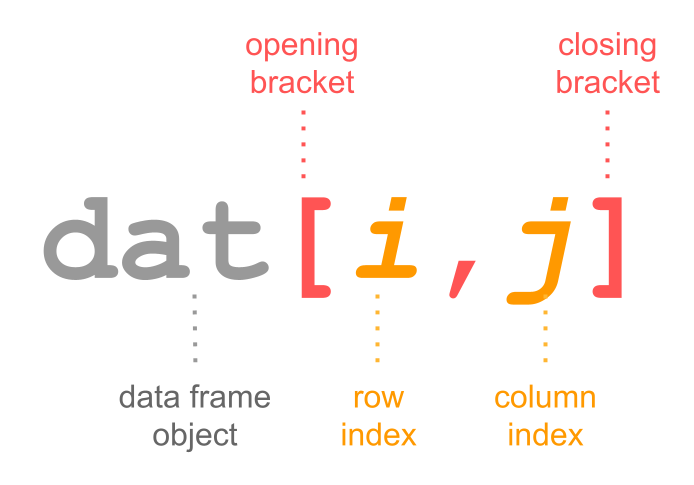
\includegraphics[width=0.5\linewidth]{images/objects/obj-dataframe-brackets} 

}

\caption{Bracket notation in data frames}\label{fig:unnamed-chunk-177}
\end{figure}

In other words, you have to specify values inside the
brackets for the 1st index, and the 2nd index: \texttt{dat{[}index1,\ index2{]}}.

\hypertarget{selecting-cells-1}{%
\subsubsection*{Selecting cells}\label{selecting-cells-1}}
\addcontentsline{toc}{subsubsection}{Selecting cells}

\begin{figure}

{\centering 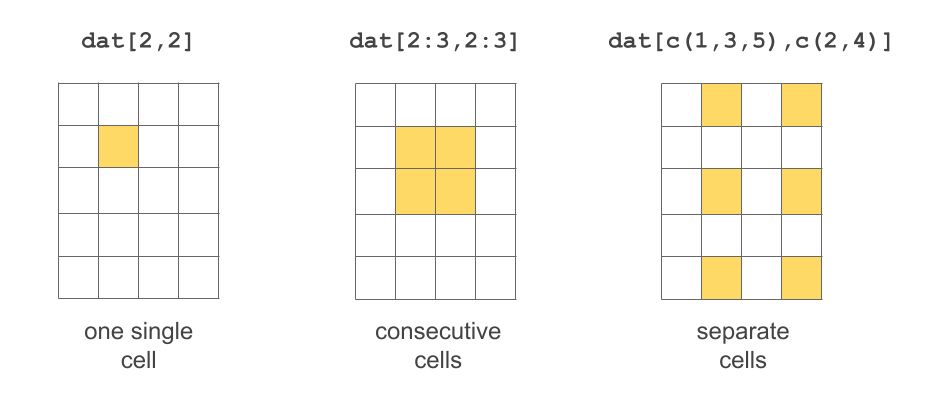
\includegraphics[width=0.8\linewidth]{images/objects/obj-dataframe-cells1} 

}

\caption{Several ways to select cells}\label{fig:unnamed-chunk-178}
\end{figure}

\begin{Shaded}
\begin{Highlighting}[]
\CommentTok{\# select value in row 1 and column 1}
\NormalTok{dat[}\DecValTok{1}\NormalTok{,}\DecValTok{1}\NormalTok{]}
\SpecialCharTok{\textgreater{}}\NormalTok{ [}\DecValTok{1}\NormalTok{] }\StringTok{"Leia"}

\CommentTok{\# select value in row 2 and column 3}
\NormalTok{dat[}\DecValTok{2}\NormalTok{,}\DecValTok{3}\NormalTok{]}
\SpecialCharTok{\textgreater{}}\NormalTok{ [}\DecValTok{1}\NormalTok{] }\FloatTok{1.72}

\CommentTok{\# select values in these cells}
\NormalTok{dat[}\DecValTok{1}\SpecialCharTok{:}\DecValTok{2}\NormalTok{,}\DecValTok{3}\SpecialCharTok{:}\DecValTok{4}\NormalTok{]}
\SpecialCharTok{\textgreater{}}\NormalTok{   height  jedi}
\SpecialCharTok{\textgreater{}} \DecValTok{1}   \FloatTok{1.50} \ConstantTok{FALSE}
\SpecialCharTok{\textgreater{}} \DecValTok{2}   \FloatTok{1.72}  \ConstantTok{TRUE}
\end{Highlighting}
\end{Shaded}

It is also possible to exclude certain rows-and-columns by passing negative
numeric indices:

\begin{figure}

{\centering 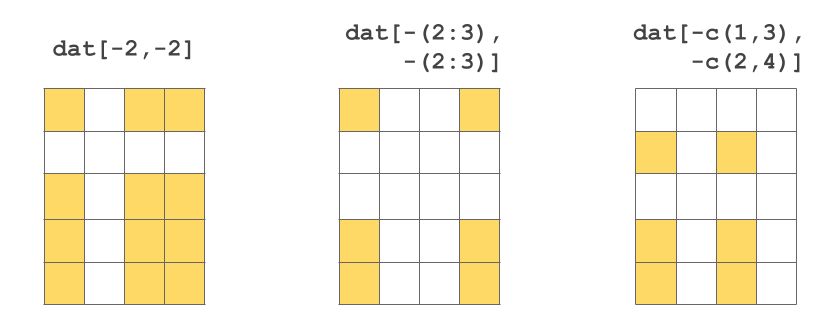
\includegraphics[width=0.8\linewidth]{images/objects/obj-dataframe-cells2} 

}

\caption{Several ways to exclude cells}\label{fig:unnamed-chunk-180}
\end{figure}

\hypertarget{selecting-rows-1}{%
\subsubsection*{Selecting rows}\label{selecting-rows-1}}
\addcontentsline{toc}{subsubsection}{Selecting rows}

\begin{figure}

{\centering 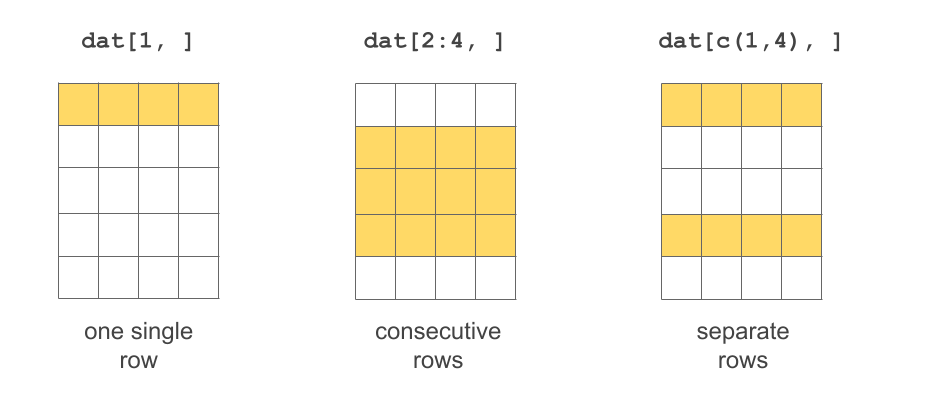
\includegraphics[width=0.8\linewidth]{images/objects/obj-dataframe-rows1} 

}

\caption{Several ways to select rows}\label{fig:unnamed-chunk-181}
\end{figure}

If no value is specified for \texttt{index1} then all rows are included. Likewise,
if no value is specified for \texttt{index2} then all columns are included.

\begin{Shaded}
\begin{Highlighting}[]
\CommentTok{\# selecting first row}
\NormalTok{dat[}\DecValTok{1}\NormalTok{, ]}
\SpecialCharTok{\textgreater{}}\NormalTok{   name gender height  jedi}
\SpecialCharTok{\textgreater{}} \DecValTok{1}\NormalTok{ Leia female    }\FloatTok{1.5} \ConstantTok{FALSE}

\CommentTok{\# selecting third row}
\NormalTok{dat[}\DecValTok{3}\NormalTok{, ]}
\SpecialCharTok{\textgreater{}}\NormalTok{   name gender height  jedi}
\SpecialCharTok{\textgreater{}} \DecValTok{3}\NormalTok{  Han   male    }\FloatTok{1.8} \ConstantTok{FALSE}
\end{Highlighting}
\end{Shaded}

\begin{figure}

{\centering 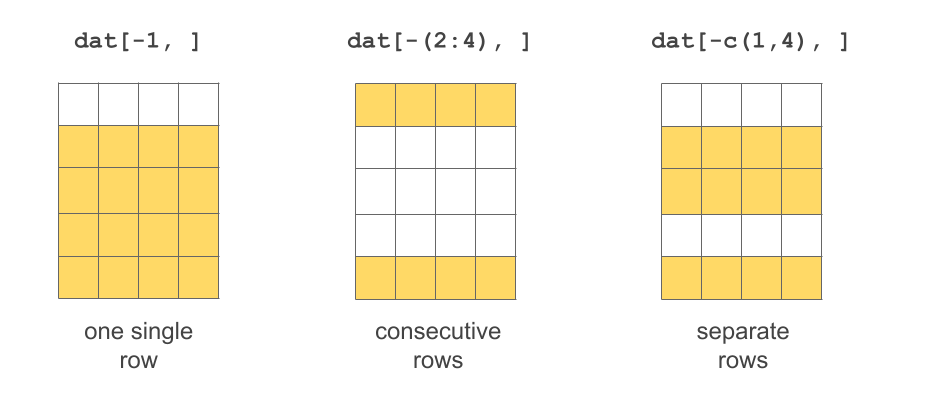
\includegraphics[width=0.8\linewidth]{images/objects/obj-dataframe-rows2} 

}

\caption{Several ways to exclude rows}\label{fig:unnamed-chunk-183}
\end{figure}

\hypertarget{selecting-columns-1}{%
\subsubsection*{Selecting columns}\label{selecting-columns-1}}
\addcontentsline{toc}{subsubsection}{Selecting columns}

\begin{figure}

{\centering 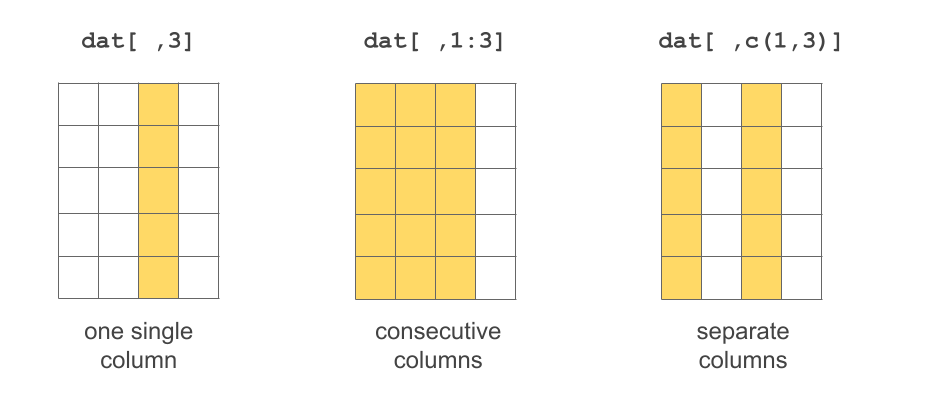
\includegraphics[width=0.8\linewidth]{images/objects/obj-dataframe-cols1} 

}

\caption{Several ways to select columns}\label{fig:unnamed-chunk-184}
\end{figure}

\begin{Shaded}
\begin{Highlighting}[]
\CommentTok{\# selecting second column}
\NormalTok{dat[ ,}\DecValTok{2}\NormalTok{]}
\SpecialCharTok{\textgreater{}}\NormalTok{ [}\DecValTok{1}\NormalTok{] }\StringTok{"female"} \StringTok{"male"}   \StringTok{"male"}

\CommentTok{\# selecting columns 2 to 4}
\NormalTok{dat[ ,}\DecValTok{2}\SpecialCharTok{:}\DecValTok{4}\NormalTok{]}
\SpecialCharTok{\textgreater{}}\NormalTok{   gender height  jedi}
\SpecialCharTok{\textgreater{}} \DecValTok{1}\NormalTok{ female   }\FloatTok{1.50} \ConstantTok{FALSE}
\SpecialCharTok{\textgreater{}} \DecValTok{2}\NormalTok{   male   }\FloatTok{1.72}  \ConstantTok{TRUE}
\SpecialCharTok{\textgreater{}} \DecValTok{3}\NormalTok{   male   }\FloatTok{1.80} \ConstantTok{FALSE}
\end{Highlighting}
\end{Shaded}

\begin{figure}

{\centering 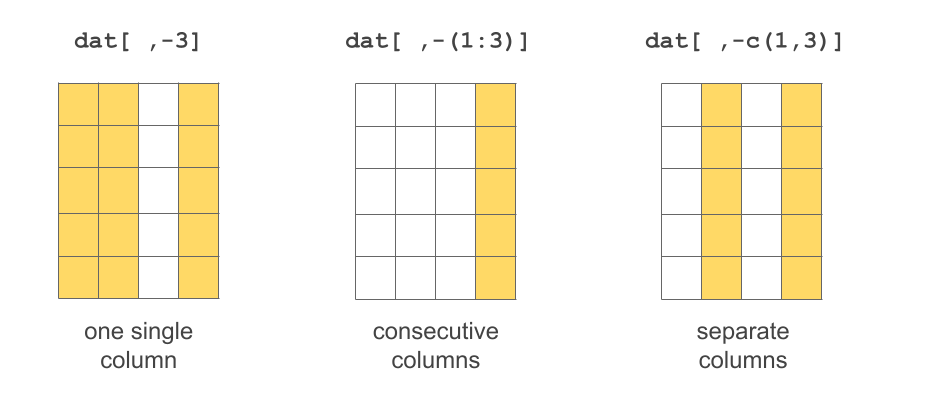
\includegraphics[width=0.8\linewidth]{images/objects/obj-dataframe-cols2} 

}

\caption{Several ways to exclude columns}\label{fig:unnamed-chunk-186}
\end{figure}

\hypertarget{more-options-to-access-columns}{%
\subsubsection*{More Options to Access Columns}\label{more-options-to-access-columns}}
\addcontentsline{toc}{subsubsection}{More Options to Access Columns}

\begin{figure}

{\centering 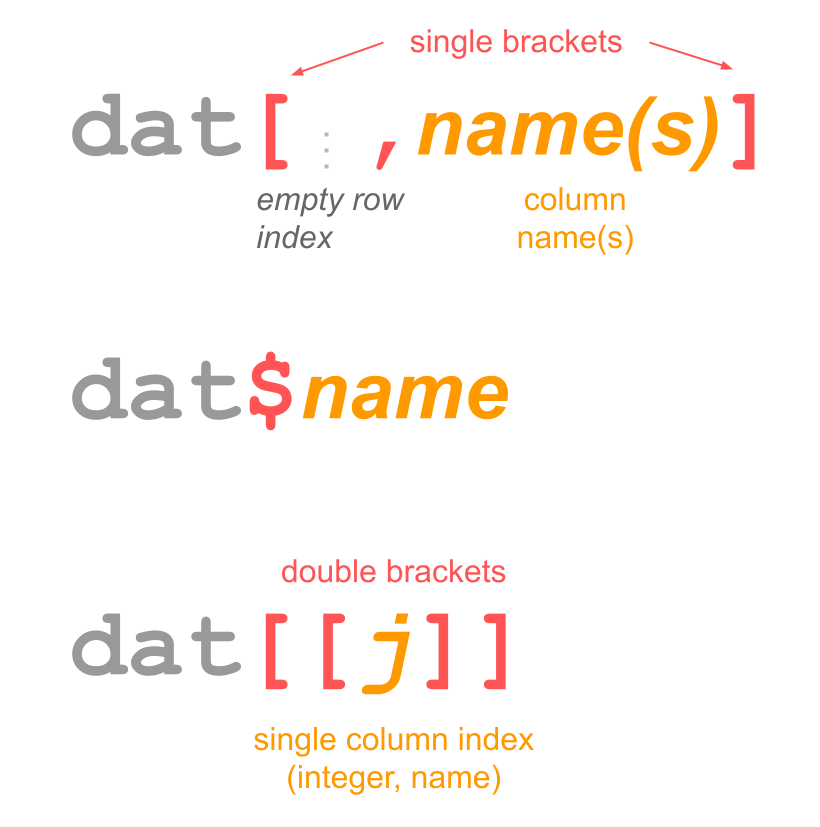
\includegraphics[width=0.5\linewidth]{images/objects/obj-dataframe-names} 

}

\caption{Other options to select columns of a data frame}\label{fig:unnamed-chunk-187}
\end{figure}

The dollar sign also works for selecting a column of a data frame
using its name

\begin{Shaded}
\begin{Highlighting}[]
\NormalTok{mtcars}\SpecialCharTok{$}\NormalTok{mpg}
\SpecialCharTok{\textgreater{}}\NormalTok{  [}\DecValTok{1}\NormalTok{] }\FloatTok{21.0} \FloatTok{21.0} \FloatTok{22.8} \FloatTok{21.4} \FloatTok{18.7} \FloatTok{18.1} \FloatTok{14.3} \FloatTok{24.4} \FloatTok{22.8}
\SpecialCharTok{\textgreater{}}\NormalTok{ [}\DecValTok{10}\NormalTok{] }\FloatTok{19.2} \FloatTok{17.8} \FloatTok{16.4} \FloatTok{17.3} \FloatTok{15.2} \FloatTok{10.4} \FloatTok{10.4} \FloatTok{14.7} \FloatTok{32.4}
\SpecialCharTok{\textgreater{}}\NormalTok{ [}\DecValTok{19}\NormalTok{] }\FloatTok{30.4} \FloatTok{33.9} \FloatTok{21.5} \FloatTok{15.5} \FloatTok{15.2} \FloatTok{13.3} \FloatTok{19.2} \FloatTok{27.3} \FloatTok{26.0}
\SpecialCharTok{\textgreater{}}\NormalTok{ [}\DecValTok{28}\NormalTok{] }\FloatTok{30.4} \FloatTok{15.8} \FloatTok{19.7} \FloatTok{15.0} \FloatTok{21.4}
\end{Highlighting}
\end{Shaded}

You don't need to use quote marks, but you can if you want. The following
calls are equivalent.

\begin{Shaded}
\begin{Highlighting}[]
\NormalTok{mtcars}\SpecialCharTok{$}\StringTok{\textquotesingle{}mpg\textquotesingle{}}
\NormalTok{mtcars}\SpecialCharTok{$}\StringTok{"mpg"}
\NormalTok{mtcars}\SpecialCharTok{$}\StringTok{\textasciigrave{}}\AttributeTok{mpg}\StringTok{\textasciigrave{}}
\end{Highlighting}
\end{Shaded}

\hypertarget{adding-a-column-1}{%
\subsection{Adding a column}\label{adding-a-column-1}}

Perhaps the simplest way to add a column is with the dollar operator \texttt{\$}.
You just need to give a name for the new column, and assign a vector (or factor):

\begin{Shaded}
\begin{Highlighting}[]
\CommentTok{\# adding a column}
\NormalTok{dat}\SpecialCharTok{$}\NormalTok{new\_column }\OtherTok{\textless{}{-}} \FunctionTok{c}\NormalTok{(}\StringTok{\textquotesingle{}a\textquotesingle{}}\NormalTok{, }\StringTok{\textquotesingle{}e\textquotesingle{}}\NormalTok{, }\StringTok{\textquotesingle{}i\textquotesingle{}}\NormalTok{)}
\NormalTok{dat}
\SpecialCharTok{\textgreater{}}\NormalTok{   name gender height  jedi new\_column}
\SpecialCharTok{\textgreater{}} \DecValTok{1}\NormalTok{ Leia female   }\FloatTok{1.50} \ConstantTok{FALSE}\NormalTok{          a}
\SpecialCharTok{\textgreater{}} \DecValTok{2}\NormalTok{ Luke   male   }\FloatTok{1.72}  \ConstantTok{TRUE}\NormalTok{          e}
\SpecialCharTok{\textgreater{}} \DecValTok{3}\NormalTok{  Han   male   }\FloatTok{1.80} \ConstantTok{FALSE}\NormalTok{          i}
\end{Highlighting}
\end{Shaded}

Another way to add a column is with the \emph{column binding} function \texttt{cbind()}:

\begin{Shaded}
\begin{Highlighting}[]
\CommentTok{\# vector of weights}
\NormalTok{weight }\OtherTok{\textless{}{-}} \FunctionTok{c}\NormalTok{(}\DecValTok{49}\NormalTok{, }\DecValTok{77}\NormalTok{, }\DecValTok{85}\NormalTok{)}

\CommentTok{\# adding weights to dat}
\NormalTok{dat }\OtherTok{\textless{}{-}} \FunctionTok{cbind}\NormalTok{(dat, weight)}
\NormalTok{dat}
\SpecialCharTok{\textgreater{}}\NormalTok{   name gender height  jedi new\_column weight}
\SpecialCharTok{\textgreater{}} \DecValTok{1}\NormalTok{ Leia female   }\FloatTok{1.50} \ConstantTok{FALSE}\NormalTok{          a     }\DecValTok{49}
\SpecialCharTok{\textgreater{}} \DecValTok{2}\NormalTok{ Luke   male   }\FloatTok{1.72}  \ConstantTok{TRUE}\NormalTok{          e     }\DecValTok{77}
\SpecialCharTok{\textgreater{}} \DecValTok{3}\NormalTok{  Han   male   }\FloatTok{1.80} \ConstantTok{FALSE}\NormalTok{          i     }\DecValTok{85}
\end{Highlighting}
\end{Shaded}

\hypertarget{deleting-a-column-1}{%
\subsection{Deleting a column}\label{deleting-a-column-1}}

The inverse operation of adding a column consists of \textbf{deleting} a column.
This is possible with the \texttt{\$} dollar operator. For instance, say you want to
remove the column \texttt{new\_column}. Use the \texttt{\$} operator to select this column,
and assign it the value \texttt{NULL} (think of this as \emph{NULLifying} a column):

\begin{Shaded}
\begin{Highlighting}[]
\CommentTok{\# deleting a column}
\NormalTok{dat}\SpecialCharTok{$}\NormalTok{new\_column }\OtherTok{\textless{}{-}} \ConstantTok{NULL}
\NormalTok{dat}
\SpecialCharTok{\textgreater{}}\NormalTok{   name gender height  jedi weight}
\SpecialCharTok{\textgreater{}} \DecValTok{1}\NormalTok{ Leia female   }\FloatTok{1.50} \ConstantTok{FALSE}     \DecValTok{49}
\SpecialCharTok{\textgreater{}} \DecValTok{2}\NormalTok{ Luke   male   }\FloatTok{1.72}  \ConstantTok{TRUE}     \DecValTok{77}
\SpecialCharTok{\textgreater{}} \DecValTok{3}\NormalTok{  Han   male   }\FloatTok{1.80} \ConstantTok{FALSE}     \DecValTok{85}
\end{Highlighting}
\end{Shaded}

\hypertarget{renaming-a-column}{%
\subsection{Renaming a column}\label{renaming-a-column}}

What if you want to rename a column? There are various options to do this.
One way is by changing the column \texttt{names} attribute:

\begin{Shaded}
\begin{Highlighting}[]
\CommentTok{\# attributes}
\FunctionTok{attributes}\NormalTok{(dat)}
\SpecialCharTok{\textgreater{}} \ErrorTok{$}\NormalTok{names}
\SpecialCharTok{\textgreater{}}\NormalTok{ [}\DecValTok{1}\NormalTok{] }\StringTok{"name"}   \StringTok{"gender"} \StringTok{"height"} \StringTok{"jedi"}   \StringTok{"weight"}
\SpecialCharTok{\textgreater{}} 
\ErrorTok{\textgreater{}} \ErrorTok{$}\NormalTok{row.names}
\SpecialCharTok{\textgreater{}}\NormalTok{ [}\DecValTok{1}\NormalTok{] }\DecValTok{1} \DecValTok{2} \DecValTok{3}
\SpecialCharTok{\textgreater{}} 
\ErrorTok{\textgreater{}} \ErrorTok{$}\NormalTok{class}
\SpecialCharTok{\textgreater{}}\NormalTok{ [}\DecValTok{1}\NormalTok{] }\StringTok{"data.frame"}
\end{Highlighting}
\end{Shaded}

which is more commonly accessed with the \texttt{names()} function:

\begin{Shaded}
\begin{Highlighting}[]
\CommentTok{\# column names}
\FunctionTok{names}\NormalTok{(dat)}
\SpecialCharTok{\textgreater{}}\NormalTok{ [}\DecValTok{1}\NormalTok{] }\StringTok{"name"}   \StringTok{"gender"} \StringTok{"height"} \StringTok{"jedi"}   \StringTok{"weight"}
\end{Highlighting}
\end{Shaded}

Notice that \texttt{dat} has a list of attributes. The element \texttt{names} is the vector
of column names.

You can directly modify the vector of \texttt{names}; for example let's change
\texttt{gender} to \texttt{sex}:

\begin{Shaded}
\begin{Highlighting}[]
\CommentTok{\# changing rookie to rooky}
\FunctionTok{attributes}\NormalTok{(dat)}\SpecialCharTok{$}\NormalTok{names[}\DecValTok{2}\NormalTok{] }\OtherTok{\textless{}{-}} \StringTok{"sex"}

\CommentTok{\# display column names}
\FunctionTok{names}\NormalTok{(dat)}
\SpecialCharTok{\textgreater{}}\NormalTok{ [}\DecValTok{1}\NormalTok{] }\StringTok{"name"}   \StringTok{"sex"}    \StringTok{"height"} \StringTok{"jedi"}   \StringTok{"weight"}
\end{Highlighting}
\end{Shaded}

By the way: this approach of changing the name of a variable is very low level,
and probably unfamiliar to most useRs.

\hypertarget{moving-a-column-1}{%
\subsection{Moving a column}\label{moving-a-column-1}}

A more challenging operation is when you want to move a column to a different
position. What if you want to move \texttt{salary} to the last position (last column)?
One option is to create a vector of column names in the desired order, and then
use this vector (for the index of columns) to reassign the data frame like this:

\begin{Shaded}
\begin{Highlighting}[]
\NormalTok{reordered\_names }\OtherTok{\textless{}{-}} \FunctionTok{c}\NormalTok{(}\StringTok{"name"}\NormalTok{, }\StringTok{"jedi"}\NormalTok{, }\StringTok{"height"}\NormalTok{, }\StringTok{"weight"}\NormalTok{, }\StringTok{"sex"}\NormalTok{)}
\NormalTok{dat }\OtherTok{\textless{}{-}}\NormalTok{ dat[ ,reordered\_names]}
\NormalTok{dat}
\SpecialCharTok{\textgreater{}}\NormalTok{   name  jedi height weight    sex}
\SpecialCharTok{\textgreater{}} \DecValTok{1}\NormalTok{ Leia }\ConstantTok{FALSE}   \FloatTok{1.50}     \DecValTok{49}\NormalTok{ female}
\SpecialCharTok{\textgreater{}} \DecValTok{2}\NormalTok{ Luke  }\ConstantTok{TRUE}   \FloatTok{1.72}     \DecValTok{77}\NormalTok{   male}
\SpecialCharTok{\textgreater{}} \DecValTok{3}\NormalTok{  Han }\ConstantTok{FALSE}   \FloatTok{1.80}     \DecValTok{85}\NormalTok{   male}
\end{Highlighting}
\end{Shaded}

\hypertarget{transforming-a-column}{%
\subsection{Transforming a column}\label{transforming-a-column}}

A more common operation than deleting or moving a column, is to transform the
values in a column. This can be easily accomplished with the \texttt{\$} operator.
For instance, let's say that we want to transform \texttt{height} from meters to
centimeters:

\begin{Shaded}
\begin{Highlighting}[]
\CommentTok{\# converting height to centimeters}
\NormalTok{dat}\SpecialCharTok{$}\NormalTok{height }\OtherTok{\textless{}{-}}\NormalTok{ dat}\SpecialCharTok{$}\NormalTok{height }\SpecialCharTok{*} \DecValTok{100}
\NormalTok{dat}
\SpecialCharTok{\textgreater{}}\NormalTok{   name  jedi height weight    sex}
\SpecialCharTok{\textgreater{}} \DecValTok{1}\NormalTok{ Leia }\ConstantTok{FALSE}    \DecValTok{150}     \DecValTok{49}\NormalTok{ female}
\SpecialCharTok{\textgreater{}} \DecValTok{2}\NormalTok{ Luke  }\ConstantTok{TRUE}    \DecValTok{172}     \DecValTok{77}\NormalTok{   male}
\SpecialCharTok{\textgreater{}} \DecValTok{3}\NormalTok{  Han }\ConstantTok{FALSE}    \DecValTok{180}     \DecValTok{85}\NormalTok{   male}
\end{Highlighting}
\end{Shaded}

Likewise, instead of using the \texttt{\$} operator, you can refer to the column using
bracket notation. Here's how to transform weight from kilograms to pounds
(1 kg = 2.20462 pounds):

\begin{Shaded}
\begin{Highlighting}[]
\CommentTok{\# weight into pounds}
\NormalTok{dat[ ,}\StringTok{"weight"}\NormalTok{] }\OtherTok{\textless{}{-}}\NormalTok{ dat[ ,}\StringTok{"weight"}\NormalTok{] }\SpecialCharTok{*} \FloatTok{2.20462}
\NormalTok{dat}
\SpecialCharTok{\textgreater{}}\NormalTok{   name  jedi height   weight    sex}
\SpecialCharTok{\textgreater{}} \DecValTok{1}\NormalTok{ Leia }\ConstantTok{FALSE}    \DecValTok{150} \FloatTok{108.0264}\NormalTok{ female}
\SpecialCharTok{\textgreater{}} \DecValTok{2}\NormalTok{ Luke  }\ConstantTok{TRUE}    \DecValTok{172} \FloatTok{169.7557}\NormalTok{   male}
\SpecialCharTok{\textgreater{}} \DecValTok{3}\NormalTok{  Han }\ConstantTok{FALSE}    \DecValTok{180} \FloatTok{187.3927}\NormalTok{   male}
\end{Highlighting}
\end{Shaded}

There is also the \texttt{transform()} function which transform values \emph{interactively},
that is, temporarily:

\begin{Shaded}
\begin{Highlighting}[]
\CommentTok{\# transform weight to kgs}
\FunctionTok{transform}\NormalTok{(dat, }\AttributeTok{weight =}\NormalTok{ weight }\SpecialCharTok{/} \FloatTok{0.453592}\NormalTok{)}
\SpecialCharTok{\textgreater{}}\NormalTok{   name  jedi height   weight    sex}
\SpecialCharTok{\textgreater{}} \DecValTok{1}\NormalTok{ Leia }\ConstantTok{FALSE}    \DecValTok{150} \FloatTok{238.1576}\NormalTok{ female}
\SpecialCharTok{\textgreater{}} \DecValTok{2}\NormalTok{ Luke  }\ConstantTok{TRUE}    \DecValTok{172} \FloatTok{374.2476}\NormalTok{   male}
\SpecialCharTok{\textgreater{}} \DecValTok{3}\NormalTok{  Han }\ConstantTok{FALSE}    \DecValTok{180} \FloatTok{413.1305}\NormalTok{   male}
\end{Highlighting}
\end{Shaded}

\texttt{transform()} does its job of modifying the values of \texttt{weight} but only
temporarily; if you inspect \texttt{dat} you'll see what this means:

\begin{Shaded}
\begin{Highlighting}[]
\CommentTok{\# did weight really change?}
\NormalTok{dat}
\SpecialCharTok{\textgreater{}}\NormalTok{   name  jedi height   weight    sex}
\SpecialCharTok{\textgreater{}} \DecValTok{1}\NormalTok{ Leia }\ConstantTok{FALSE}    \DecValTok{150} \FloatTok{108.0264}\NormalTok{ female}
\SpecialCharTok{\textgreater{}} \DecValTok{2}\NormalTok{ Luke  }\ConstantTok{TRUE}    \DecValTok{172} \FloatTok{169.7557}\NormalTok{   male}
\SpecialCharTok{\textgreater{}} \DecValTok{3}\NormalTok{  Han }\ConstantTok{FALSE}    \DecValTok{180} \FloatTok{187.3927}\NormalTok{   male}
\end{Highlighting}
\end{Shaded}

To make the changes permanent with \texttt{transform()}, you need to reassign them
to the data frame:

\begin{Shaded}
\begin{Highlighting}[]
\CommentTok{\# transform weight to inches (permanently)}
\NormalTok{dat }\OtherTok{\textless{}{-}} \FunctionTok{transform}\NormalTok{(dat, }\AttributeTok{weight =}\NormalTok{ weight }\SpecialCharTok{/} \FloatTok{0.453592}\NormalTok{)}
\NormalTok{dat}
\SpecialCharTok{\textgreater{}}\NormalTok{   name  jedi height   weight    sex}
\SpecialCharTok{\textgreater{}} \DecValTok{1}\NormalTok{ Leia }\ConstantTok{FALSE}    \DecValTok{150} \FloatTok{238.1576}\NormalTok{ female}
\SpecialCharTok{\textgreater{}} \DecValTok{2}\NormalTok{ Luke  }\ConstantTok{TRUE}    \DecValTok{172} \FloatTok{374.2476}\NormalTok{   male}
\SpecialCharTok{\textgreater{}} \DecValTok{3}\NormalTok{  Han }\ConstantTok{FALSE}    \DecValTok{180} \FloatTok{413.1305}\NormalTok{   male}
\end{Highlighting}
\end{Shaded}

\begin{center}\rule{0.5\linewidth}{0.5pt}\end{center}

\hypertarget{exercises-6}{%
\section{Exercises}\label{exercises-6}}

\textbf{1)} Consider the following data frame \texttt{df}:

\begin{verbatim}
      first      last  gender  born         spell
1     Harry    Potter    male  1980  sectumsempra
2  Hermione   Granger  female  1979     alohomora
3       Ron   Weasley    male  1980    riddikulus
4      Luna  Lovegood  female  1981       episkey
\end{verbatim}

\begin{enumerate}
\def\labelenumi{\alph{enumi})}
\item
  What commands will fail to return the data of individuals born in 1980?

  \begin{enumerate}
  \def\labelenumii{\roman{enumii})}
  \item
    \texttt{df{[}c(TRUE,\ FALSE,\ TRUE,\ FALSE),\ {]}}
  \item
    \texttt{df{[}df{[},4{]}\ ==\ 1980,\ {]}}
  \item
    \texttt{df{[}df\$born\ ==\ 1980{]}}
  \item
    \texttt{df{[}df\$born\ ==\ 1980,\ {]}}
  \item
    \texttt{df{[}\ ,df\$born\ ==\ 1980{]}}
  \end{enumerate}
\item
  Select the command that does \textbf{not} provide information about the data
  frame \texttt{df}:

  \begin{enumerate}
  \def\labelenumii{\roman{enumii})}
  \item
    \texttt{head(df)}
  \item
    \texttt{str(df)}
  \item
    \texttt{tail(df)}
  \item
    \texttt{rm(df)}
  \item
    \texttt{summary(df)}
  \end{enumerate}
\item
  Your friend is trying to display the first three rows on columns 1 (\texttt{first})
  and 2 (\texttt{last}), by unsuccessfully using the following command.
  Why does the command print all columns?
\end{enumerate}

\begin{Shaded}
\begin{Highlighting}[]
\NormalTok{df[}\DecValTok{1}\SpecialCharTok{:}\DecValTok{3}\NormalTok{, }\DecValTok{1} \SpecialCharTok{\&} \DecValTok{2}\NormalTok{]}
\SpecialCharTok{\textgreater{}}\NormalTok{      first    last gender born        spell}
\SpecialCharTok{\textgreater{}} \DecValTok{1}\NormalTok{    Harry  Potter   male }\DecValTok{1980}\NormalTok{ sectumsempra}
\SpecialCharTok{\textgreater{}} \DecValTok{2}\NormalTok{ Hermione Granger female }\DecValTok{1979}\NormalTok{    alohomora}
\SpecialCharTok{\textgreater{}} \DecValTok{3}\NormalTok{      Ron Weasley   male }\DecValTok{1980}\NormalTok{   riddikulus}
\end{Highlighting}
\end{Shaded}

\begin{enumerate}
\def\labelenumi{\alph{enumi})}
\setcounter{enumi}{3}
\item
  Write a command that would correctly display the first two columns.
\item
  Write a command that would give you the following data from \texttt{df}.
\end{enumerate}

\begin{verbatim}
         spell    first
1 sectumsempra    Harry
2    alohomora Hermione
3   riddikulus      Ron
4      episkey     Luna
\end{verbatim}

\textbf{2)} Consider the following data frame \texttt{dat}

\begin{verbatim}
       first        last   gender      title
1        Jon        Snow     male       lord
2       Arya       Stark   female   princess
3     Tyrion   Lannister     male     master
4   Daenerys   Targaryen   female   khaleesi
5       Yara     Greyjoy   female   princess
    gpa
1   2.8
2   3.5
3   2.9
4   3.7
5    NA
\end{verbatim}

One of your friends wrote the following R code. Help your friend find all the
errors and \textbf{explain what's wrong}.

\begin{verbatim}
# value of 'first' associated to maximum 'gpa'
max_gpa <- max(dat$gpa, na.rm = TRUE)
which_max_gpa <- dat$gpa = max_gpa
dat$first(which_max_gpa)

# gpa of title lord
dat$gpa[dat[ ,title] = "lord"]

# median gpa (of each gender)
which_males <- dat$gender == 'male'
which_females <- dat$gender == 'female'
median_females <- median(dat$gpa[which_males])
median_males <- median(dat$gpa[which_males])
\end{verbatim}

\hypertarget{part-graphics}{%
\part{Graphics}\label{part-graphics}}

\hypertarget{graphics1}{%
\chapter{Base Graphics}\label{graphics1}}

R comes with many functions that let us produce a wide variety of graphics,
plots, diagrams, charts, maps, \ldots{} you name it.

In this chapter we'll describe the traditional system to produce plots using
functions from the underlying package \texttt{"graphics"}.

\hypertarget{basics-of-graphics-in-r}{%
\section{Basics of Graphics in R}\label{basics-of-graphics-in-r}}

The package \texttt{"graphics"} is the traditional system; it provides functions for
complete plots, as well as low-level facilities.

Many other graphics packages are built on top of \texttt{"graphics"} like \texttt{"maps"},
\texttt{"diagram"}, \texttt{"pixmap"}, and many more.

Graphics functions can be divided into two main types:

\begin{itemize}
\item
  \textbf{high-level} functions produce complete plots, for example

  \begin{itemize}
  \tightlist
  \item
    \texttt{barplot()}
  \item
    \texttt{hist()}
  \item
    \texttt{boxplot()}
  \item
    \texttt{dotchart()}
  \end{itemize}
\item
  \textbf{low-level} functions add further output to an existing plot

  \begin{itemize}
  \tightlist
  \item
    \texttt{text()}
  \item
    \texttt{points()}
  \item
    \texttt{lines()}
  \item
    \texttt{legend()}
  \item
    \emph{etc}
  \end{itemize}
\end{itemize}

About R graphics:

\begin{itemize}
\item
  R \texttt{"graphics"} follow a static, ``painting on canvas'' model.
\item
  Graphics elements are drawn, and remain visible until painted over.
\item
  For dynamic and/or interactive graphics, R is limited. However, several
  packages have been (and continue to be) developed in order to provide more
  flexibility and interactivity.
\end{itemize}

\hypertarget{the-plot-function}{%
\section{\texorpdfstring{The \texttt{plot()} function}{The plot() function}}\label{the-plot-function}}

\texttt{plot()} is the most important high-level function in traditional graphics

\begin{itemize}
\item
  The first argument to \texttt{plot()} provides the data to plot
\item
  The provided data can take different forms: e.g.~vectors, factors, matrices,
  data frames.
\item
  To be more precise, \texttt{plot()} is a generic function
\item
  You can create your own \texttt{plot()} method function
\end{itemize}

In its basic form, we can use \texttt{plot()} to make graphics of:

\begin{itemize}
\item
  one single variable
\item
  two variables
\item
  multiple variables
\end{itemize}

\hypertarget{traditional-graphics-in-r}{%
\section{Traditional Graphics in R}\label{traditional-graphics-in-r}}

In the traditional model, we create a plot by first calling a high-level
function that creates a complete plot, and then we call low-level functions
to add more output if necessary

Consider the data set \texttt{mtcars} (a few rows shown below)

\begin{Shaded}
\begin{Highlighting}[]
\FunctionTok{head}\NormalTok{(mtcars)}
\NormalTok{                   mpg cyl disp  hp drat    wt}
\NormalTok{Mazda RX4         }\FloatTok{21.0}   \DecValTok{6}  \DecValTok{160} \DecValTok{110} \FloatTok{3.90} \FloatTok{2.620}
\NormalTok{Mazda RX4 Wag     }\FloatTok{21.0}   \DecValTok{6}  \DecValTok{160} \DecValTok{110} \FloatTok{3.90} \FloatTok{2.875}
\NormalTok{Datsun }\DecValTok{710}        \FloatTok{22.8}   \DecValTok{4}  \DecValTok{108}  \DecValTok{93} \FloatTok{3.85} \FloatTok{2.320}
\NormalTok{Hornet }\DecValTok{4}\NormalTok{ Drive    }\FloatTok{21.4}   \DecValTok{6}  \DecValTok{258} \DecValTok{110} \FloatTok{3.08} \FloatTok{3.215}
\NormalTok{Hornet Sportabout }\FloatTok{18.7}   \DecValTok{8}  \DecValTok{360} \DecValTok{175} \FloatTok{3.15} \FloatTok{3.440}
\NormalTok{Valiant           }\FloatTok{18.1}   \DecValTok{6}  \DecValTok{225} \DecValTok{105} \FloatTok{2.76} \FloatTok{3.460}
\NormalTok{                   qsec vs am gear carb}
\NormalTok{Mazda RX4         }\FloatTok{16.46}  \DecValTok{0}  \DecValTok{1}    \DecValTok{4}    \DecValTok{4}
\NormalTok{Mazda RX4 Wag     }\FloatTok{17.02}  \DecValTok{0}  \DecValTok{1}    \DecValTok{4}    \DecValTok{4}
\NormalTok{Datsun }\DecValTok{710}        \FloatTok{18.61}  \DecValTok{1}  \DecValTok{1}    \DecValTok{4}    \DecValTok{1}
\NormalTok{Hornet }\DecValTok{4}\NormalTok{ Drive    }\FloatTok{19.44}  \DecValTok{1}  \DecValTok{0}    \DecValTok{3}    \DecValTok{1}
\NormalTok{Hornet Sportabout }\FloatTok{17.02}  \DecValTok{0}  \DecValTok{0}    \DecValTok{3}    \DecValTok{2}
\NormalTok{Valiant           }\FloatTok{20.22}  \DecValTok{1}  \DecValTok{0}    \DecValTok{3}    \DecValTok{1}
\end{Highlighting}
\end{Shaded}

Let's start with a scatterplot of \texttt{hp} (horse power) and \texttt{mpg} (miles per
gallon). Perhaps the most common way to get this graph is with the high-level
function \texttt{plot()}

\begin{Shaded}
\begin{Highlighting}[]
\CommentTok{\# simple scatter{-}plot}
\FunctionTok{plot}\NormalTok{(mtcars}\SpecialCharTok{$}\NormalTok{mpg, mtcars}\SpecialCharTok{$}\NormalTok{hp)}
\end{Highlighting}
\end{Shaded}

\begin{center}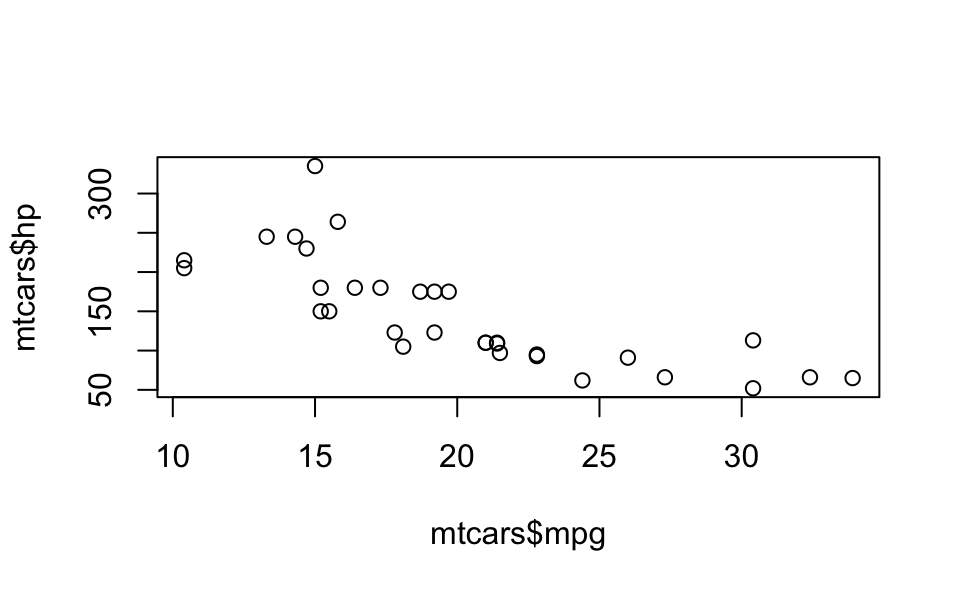
\includegraphics[width=0.7\linewidth]{R-coding-basics_files/figure-latex/unnamed-chunk-207-1} \end{center}

We can specify values for its large number of arguments. For instance, we
can set better axis names with \texttt{xlab} and \texttt{ylab}

\begin{Shaded}
\begin{Highlighting}[]
\CommentTok{\# x{-}axis and y{-}axis labels}
\FunctionTok{plot}\NormalTok{(mtcars}\SpecialCharTok{$}\NormalTok{mpg, mtcars}\SpecialCharTok{$}\NormalTok{hp, }
     \AttributeTok{xlab =} \StringTok{"miles per gallon"}\NormalTok{,}
     \AttributeTok{ylab =} \StringTok{"horsepower"}\NormalTok{)}
\end{Highlighting}
\end{Shaded}

\begin{center}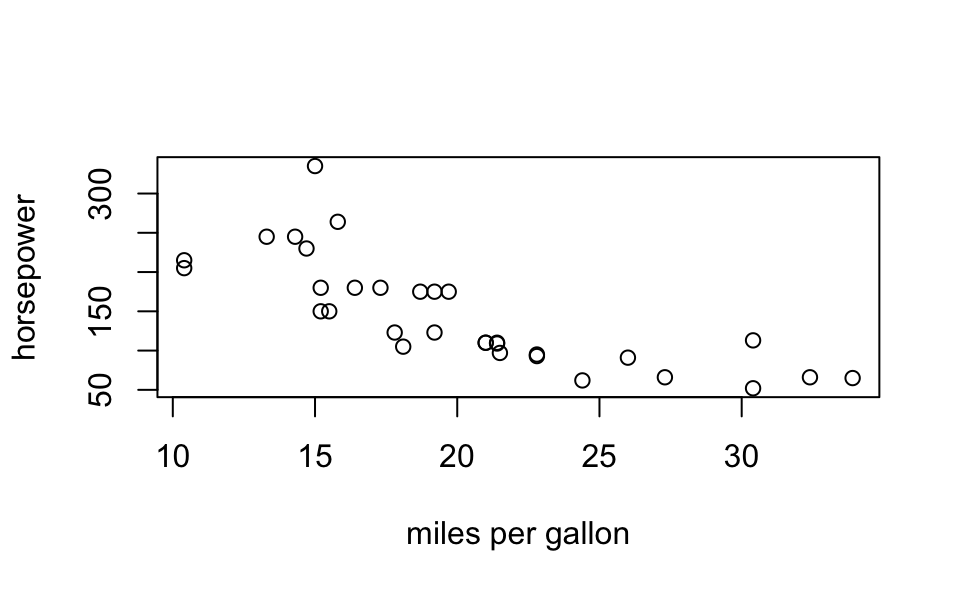
\includegraphics[width=0.7\linewidth]{R-coding-basics_files/figure-latex/unnamed-chunk-208-1} \end{center}

Likewise, we can add a title with the \texttt{main} argument:

\begin{Shaded}
\begin{Highlighting}[]
\CommentTok{\# title and subtitle}
\FunctionTok{plot}\NormalTok{(mtcars}\SpecialCharTok{$}\NormalTok{mpg, mtcars}\SpecialCharTok{$}\NormalTok{hp, }
     \AttributeTok{xlab =} \StringTok{"miles per gallon"}\NormalTok{, }\AttributeTok{ylab =} \StringTok{"horsepower"}\NormalTok{, }
     \AttributeTok{main =} \StringTok{"Simple Scatterplot"}\NormalTok{, }\AttributeTok{sub =} \StringTok{\textquotesingle{}data matcars\textquotesingle{}}\NormalTok{)}
\end{Highlighting}
\end{Shaded}

\begin{center}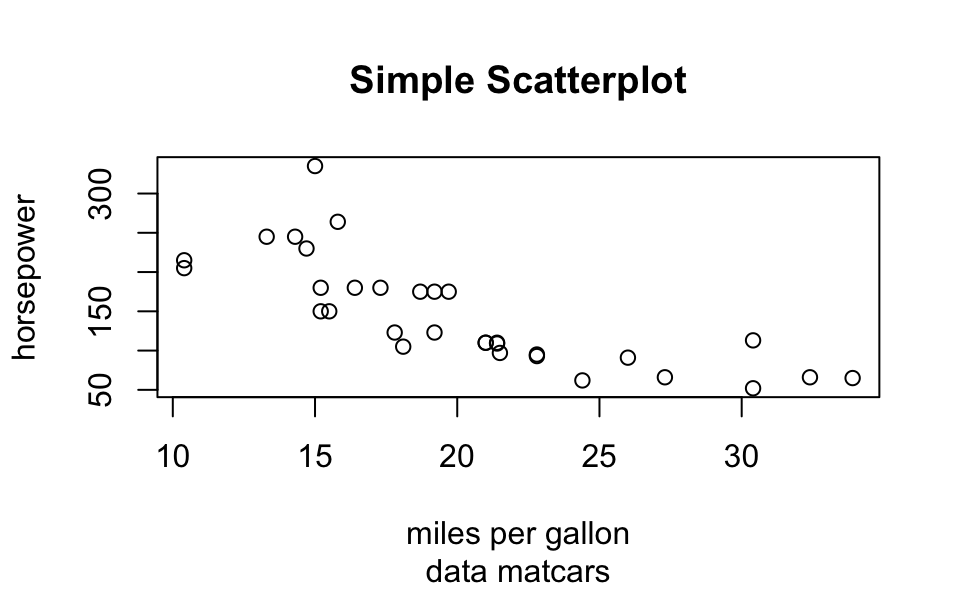
\includegraphics[width=0.7\linewidth]{R-coding-basics_files/figure-latex/unnamed-chunk-209-1} \end{center}

Or we can change the range of x-axis as well as the range of the y-axis
with \texttt{xlim} and \texttt{ylim}, respectively:

\begin{Shaded}
\begin{Highlighting}[]
\CommentTok{\# \textquotesingle{}xlim\textquotesingle{} and \textquotesingle{}ylim\textquotesingle{}}
\FunctionTok{plot}\NormalTok{(mtcars}\SpecialCharTok{$}\NormalTok{mpg, mtcars}\SpecialCharTok{$}\NormalTok{hp, }
     \AttributeTok{xlab =} \StringTok{"miles per gallon"}\NormalTok{, }\AttributeTok{ylab =} \StringTok{"horsepower"}\NormalTok{, }
     \AttributeTok{main =} \StringTok{"Simple Scatterplot"}\NormalTok{, }\AttributeTok{sub =} \StringTok{\textquotesingle{}data matcars\textquotesingle{}}\NormalTok{,}
     \AttributeTok{xlim =} \FunctionTok{c}\NormalTok{(}\DecValTok{10}\NormalTok{, }\DecValTok{35}\NormalTok{), }\AttributeTok{ylim =} \FunctionTok{c}\NormalTok{(}\DecValTok{50}\NormalTok{, }\DecValTok{400}\NormalTok{))}
\end{Highlighting}
\end{Shaded}

\begin{center}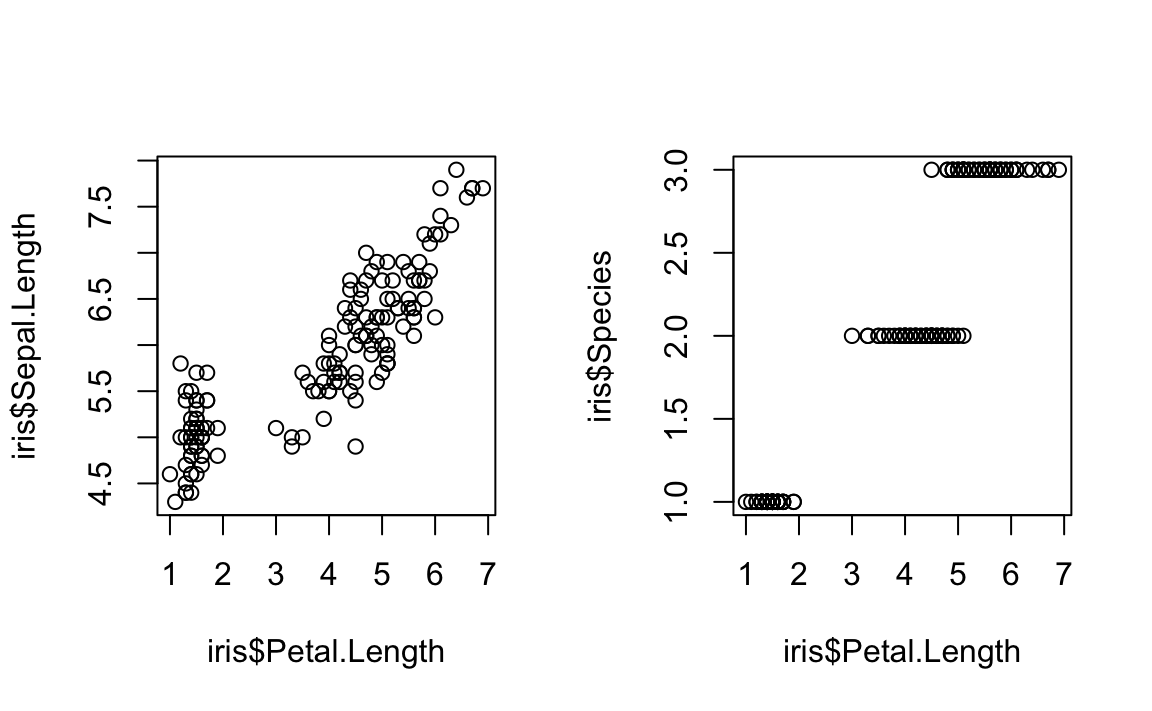
\includegraphics[width=0.7\linewidth]{R-coding-basics_files/figure-latex/unnamed-chunk-210-1} \end{center}

Here's a more sophisticated example

\begin{Shaded}
\begin{Highlighting}[]
\CommentTok{\# using plot()}
\FunctionTok{plot}\NormalTok{(mtcars}\SpecialCharTok{$}\NormalTok{mpg, }
\NormalTok{     mtcars}\SpecialCharTok{$}\NormalTok{hp, }
     \AttributeTok{xlim =} \FunctionTok{c}\NormalTok{(}\DecValTok{10}\NormalTok{, }\DecValTok{35}\NormalTok{), }
     \AttributeTok{ylim =} \FunctionTok{c}\NormalTok{(}\DecValTok{50}\NormalTok{, }\DecValTok{400}\NormalTok{),}
     \AttributeTok{xlab =} \StringTok{"miles per gallon"}\NormalTok{,}
     \AttributeTok{ylab =} \StringTok{"horsepower"}\NormalTok{, }
     \AttributeTok{main =} \StringTok{"Simple Scatterplot"}\NormalTok{,}
     \AttributeTok{sub =} \StringTok{"data matcars"}\NormalTok{, }
     \AttributeTok{pch =} \DecValTok{1}\SpecialCharTok{:}\DecValTok{25}\NormalTok{, }
     \AttributeTok{cex =} \FloatTok{1.2}\NormalTok{, }
     \AttributeTok{col =} \StringTok{"blue"}\NormalTok{)}
\end{Highlighting}
\end{Shaded}

\begin{center}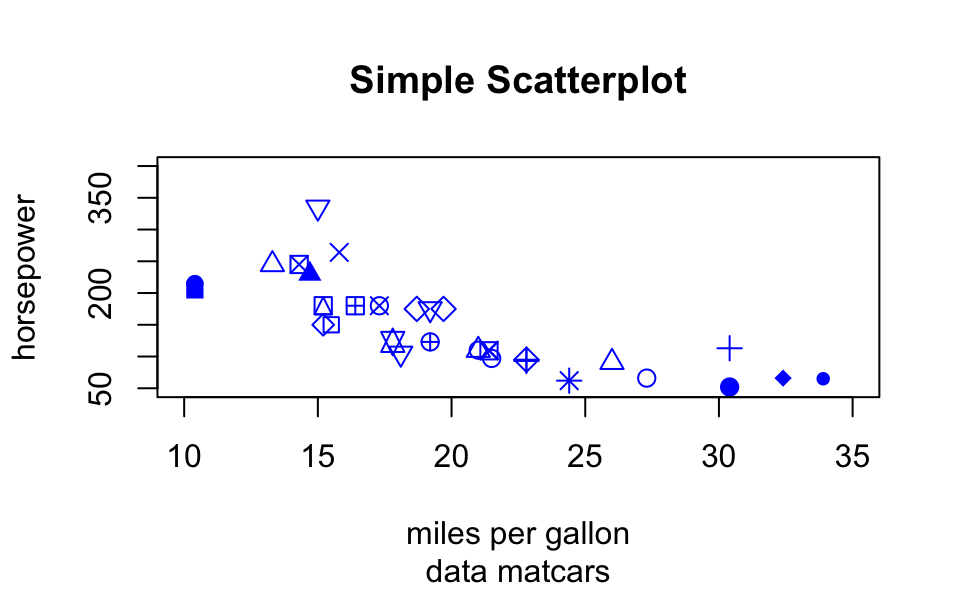
\includegraphics[width=0.7\linewidth,height=0.85\textheight]{R-coding-basics_files/figure-latex/plot_mtcars-1} \end{center}

\hypertarget{low-level-functions}{%
\section{Low-Level Functions}\label{low-level-functions}}

High and Low level functions

\begin{itemize}
\item
  Usually we call a high-level function
\item
  Most times we change the default arguments
\item
  Then we call low-level functions
\end{itemize}

Example:

\begin{Shaded}
\begin{Highlighting}[]
\CommentTok{\# simple scatter{-}plot}
\FunctionTok{plot}\NormalTok{(mtcars}\SpecialCharTok{$}\NormalTok{mpg, mtcars}\SpecialCharTok{$}\NormalTok{hp)}

\CommentTok{\# adding text}
\FunctionTok{text}\NormalTok{(mtcars}\SpecialCharTok{$}\NormalTok{mpg, mtcars}\SpecialCharTok{$}\NormalTok{hp, }\AttributeTok{labels =} \FunctionTok{rownames}\NormalTok{(mtcars))}

\CommentTok{\# dummy legend}
\FunctionTok{legend}\NormalTok{(}\StringTok{"topright"}\NormalTok{, }\AttributeTok{legend =} \StringTok{"a legend"}\NormalTok{)}

\CommentTok{\# graphic title}
\FunctionTok{title}\NormalTok{(}\StringTok{"Miles Per Galon {-}vs{-} Horsepower"}\NormalTok{)}
\end{Highlighting}
\end{Shaded}

\begin{center}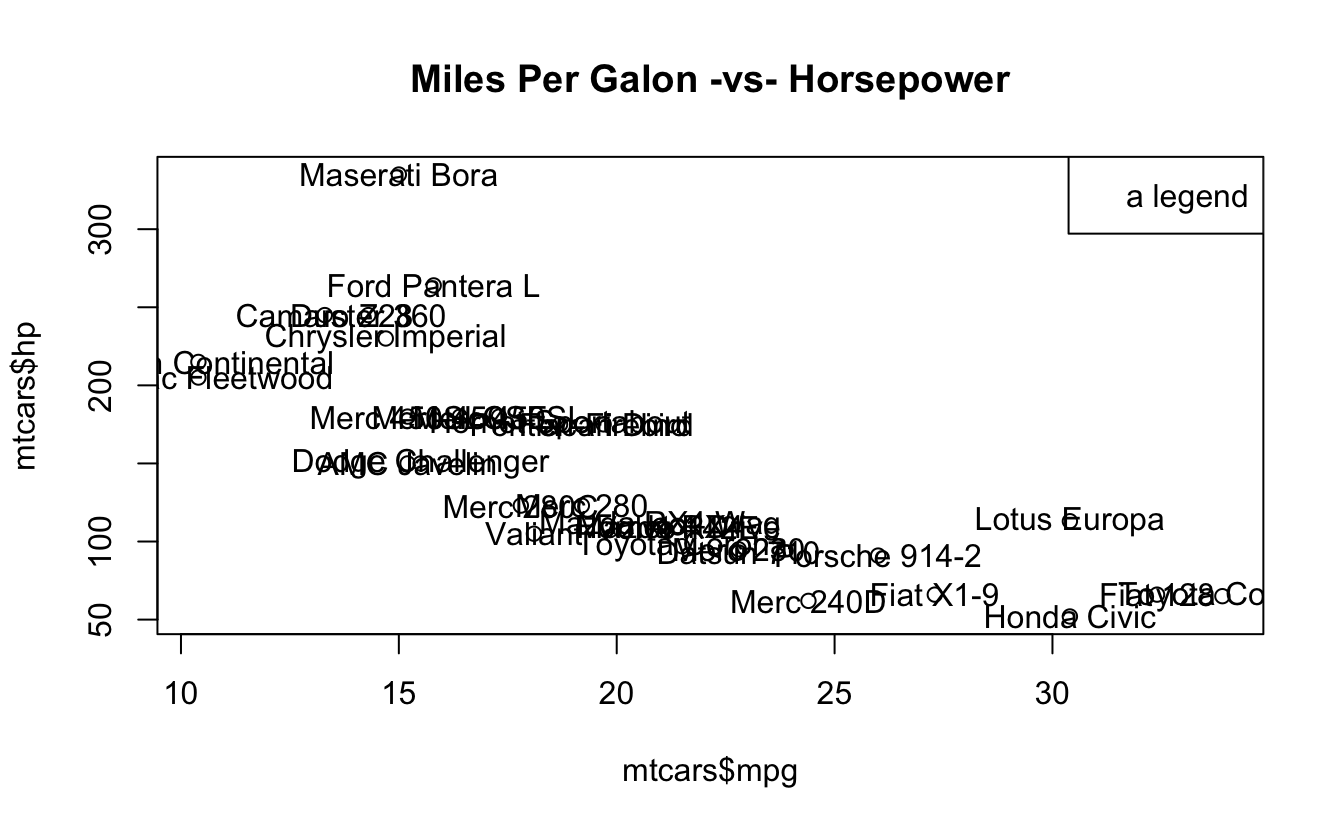
\includegraphics[width=0.7\linewidth,height=0.85\textheight]{R-coding-basics_files/figure-latex/mtcars_plot1-1} \end{center}

Another example:

\begin{Shaded}
\begin{Highlighting}[]
\CommentTok{\# simple scatter{-}plot}
\FunctionTok{plot}\NormalTok{(mtcars}\SpecialCharTok{$}\NormalTok{mpg, mtcars}\SpecialCharTok{$}\NormalTok{hp, }\AttributeTok{type =} \StringTok{"n"}\NormalTok{, }
     \AttributeTok{xlab =} \StringTok{"miles per gallon"}\NormalTok{, }\AttributeTok{ylab =} \StringTok{"horsepower"}\NormalTok{)}
\CommentTok{\# grid lines}
\FunctionTok{abline}\NormalTok{(}\AttributeTok{v =} \FunctionTok{seq}\NormalTok{(}\AttributeTok{from =} \DecValTok{10}\NormalTok{, }\AttributeTok{to =} \DecValTok{30}\NormalTok{, }\AttributeTok{by =} \DecValTok{5}\NormalTok{), }\AttributeTok{col =} \StringTok{\textquotesingle{}gray\textquotesingle{}}\NormalTok{)}
\FunctionTok{abline}\NormalTok{(}\AttributeTok{h =} \FunctionTok{seq}\NormalTok{(}\AttributeTok{from =} \DecValTok{50}\NormalTok{, }\AttributeTok{to =} \DecValTok{300}\NormalTok{, }\AttributeTok{by =} \DecValTok{50}\NormalTok{), }\AttributeTok{col =} \StringTok{\textquotesingle{} gray\textquotesingle{}}\NormalTok{)}
\CommentTok{\# plot points}
\FunctionTok{points}\NormalTok{(mtcars}\SpecialCharTok{$}\NormalTok{mpg, mtcars}\SpecialCharTok{$}\NormalTok{hp, }\AttributeTok{pch =} \DecValTok{19}\NormalTok{, }\AttributeTok{col =} \StringTok{"blue"}\NormalTok{)}
\CommentTok{\# plot text}
\FunctionTok{text}\NormalTok{(mtcars}\SpecialCharTok{$}\NormalTok{mpg, mtcars}\SpecialCharTok{$}\NormalTok{hp, }\AttributeTok{labels =} \FunctionTok{rownames}\NormalTok{(mtcars),}
     \AttributeTok{pos =} \DecValTok{4}\NormalTok{, }\AttributeTok{col =} \StringTok{"gray50"}\NormalTok{)}
\CommentTok{\# graphic title}
\FunctionTok{title}\NormalTok{(}\StringTok{"Miles Per Galon {-}vs{-} Horsepower"}\NormalTok{)}
\end{Highlighting}
\end{Shaded}

\begin{center}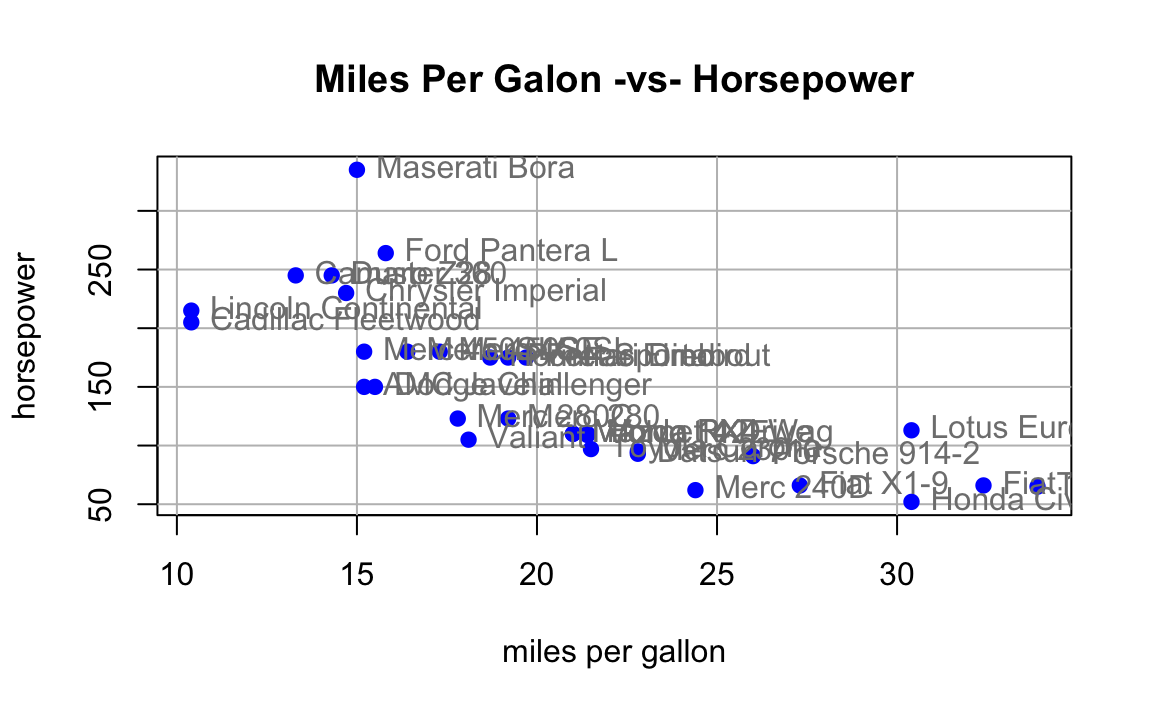
\includegraphics[width=0.7\linewidth,height=0.85\textheight]{R-coding-basics_files/figure-latex/mtcars_plot2-1} \end{center}

\hypertarget{low-level-functions-1}{%
\subsection{Low-level functions}\label{low-level-functions-1}}

\begin{longtable}[]{@{}ll@{}}
\toprule()
Function & Description \\
\midrule()
\endhead
\texttt{points()} & points \\
\texttt{lines()} & connected line segments \\
\texttt{abline()} & straight lines across a plot \\
\texttt{segments()} & disconnected line segments \\
\texttt{arrows()} & arrows \\
\texttt{rect()} & rectangles \\
\texttt{polygon()} & polygons \\
\texttt{text()} & text \\
\texttt{symbols()} & various symbols \\
\texttt{legend()} & legends \\
\bottomrule()
\end{longtable}

\hypertarget{lines}{%
\subsubsection*{Lines}\label{lines}}
\addcontentsline{toc}{subsubsection}{Lines}

\begin{Shaded}
\begin{Highlighting}[]
\NormalTok{x }\OtherTok{\textless{}{-}} \DecValTok{2005}\SpecialCharTok{:}\DecValTok{2015}

\NormalTok{y }\OtherTok{\textless{}{-}} \FunctionTok{c}\NormalTok{(}\DecValTok{81}\NormalTok{, }\DecValTok{83}\NormalTok{, }\FloatTok{84.3}\NormalTok{, }\DecValTok{85}\NormalTok{, }\FloatTok{85.4}\NormalTok{, }\FloatTok{86.5}\NormalTok{, }\FloatTok{88.3}\NormalTok{, }
       \FloatTok{88.6}\NormalTok{, }\FloatTok{90.8}\NormalTok{, }\FloatTok{91.1}\NormalTok{, }\FloatTok{91.3}\NormalTok{)}

\FunctionTok{plot}\NormalTok{(x, y, }\AttributeTok{type =} \StringTok{\textquotesingle{}n\textquotesingle{}}\NormalTok{, }\AttributeTok{xlab =} \StringTok{"Time"}\NormalTok{, }\AttributeTok{ylab =} \StringTok{"Values"}\NormalTok{)}
\FunctionTok{lines}\NormalTok{(x, y, }\AttributeTok{lwd =} \DecValTok{2}\NormalTok{)}
\FunctionTok{title}\NormalTok{(}\AttributeTok{main =} \StringTok{"Line Graph Example"}\NormalTok{)}
\end{Highlighting}
\end{Shaded}

\begin{center}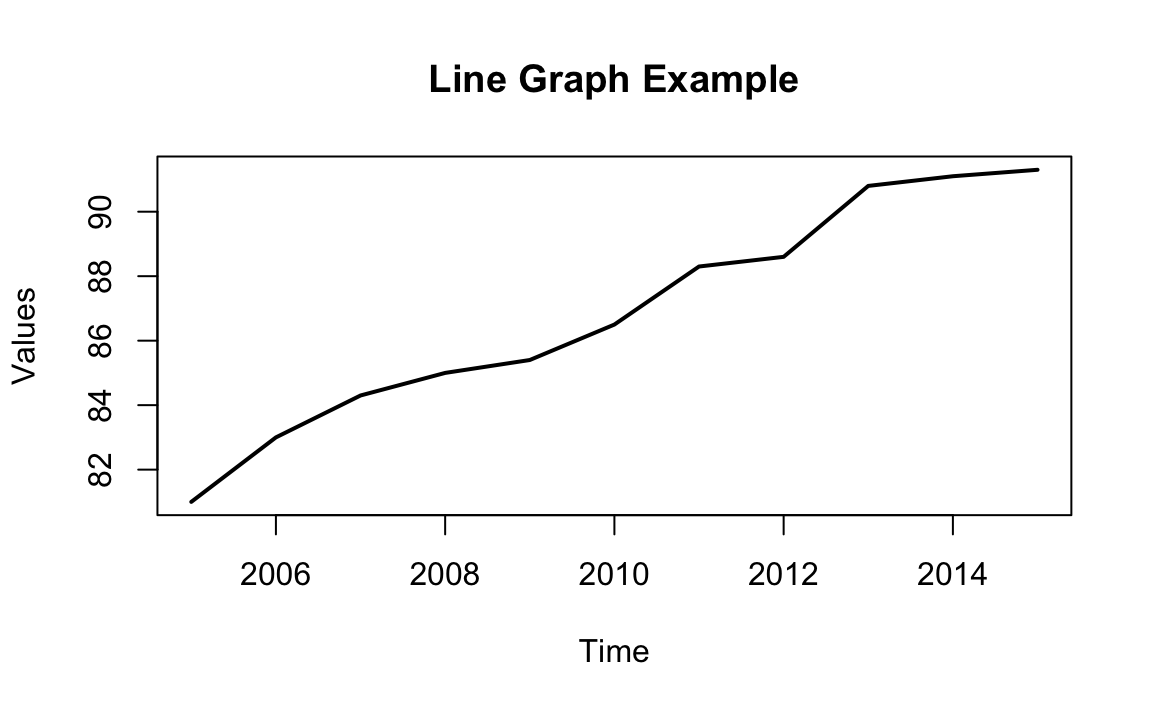
\includegraphics[width=0.7\linewidth,height=0.8\textheight]{R-coding-basics_files/figure-latex/line_segs-1} \end{center}

\hypertarget{drawing-line-segments}{%
\subsubsection{Drawing Line Segments}\label{drawing-line-segments}}

\begin{Shaded}
\begin{Highlighting}[]
\NormalTok{n }\OtherTok{\textless{}{-}} \DecValTok{11}
\NormalTok{theta }\OtherTok{\textless{}{-}} \FunctionTok{seq}\NormalTok{(}\DecValTok{0}\NormalTok{, }\DecValTok{2} \SpecialCharTok{*}\NormalTok{ pi, }\AttributeTok{length =}\NormalTok{ n }\SpecialCharTok{+} \DecValTok{1}\NormalTok{)[}\DecValTok{1}\SpecialCharTok{:}\NormalTok{n]}
\NormalTok{x }\OtherTok{\textless{}{-}} \FunctionTok{sin}\NormalTok{(theta)}
\NormalTok{y }\OtherTok{\textless{}{-}} \FunctionTok{cos}\NormalTok{(theta)}
\NormalTok{v1 }\OtherTok{\textless{}{-}} \FunctionTok{rep}\NormalTok{(}\DecValTok{1}\SpecialCharTok{:}\NormalTok{n, n)}
\NormalTok{v2 }\OtherTok{\textless{}{-}} \FunctionTok{rep}\NormalTok{(}\DecValTok{1}\SpecialCharTok{:}\NormalTok{n, }\FunctionTok{rep}\NormalTok{(n, n))}

\FunctionTok{plot}\NormalTok{(x, y, }\AttributeTok{type =} \StringTok{\textquotesingle{}n\textquotesingle{}}\NormalTok{)}
\FunctionTok{segments}\NormalTok{(x[v1], y[v1], x[v2], y[v2])}
\end{Highlighting}
\end{Shaded}

\begin{center}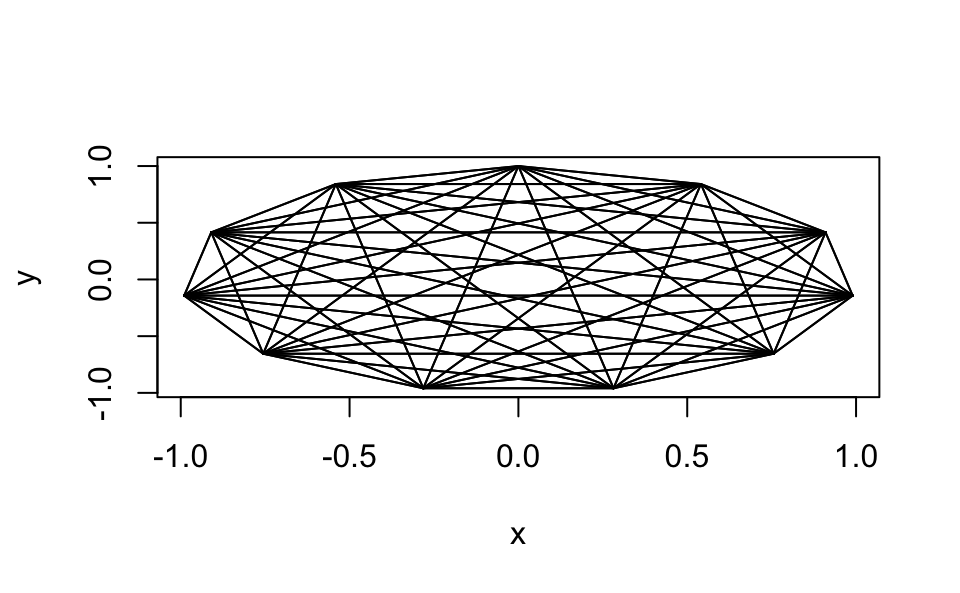
\includegraphics[width=0.7\linewidth,height=0.8\textheight]{R-coding-basics_files/figure-latex/segments-1} \end{center}

\hypertarget{drawing-polygons}{%
\subsubsection*{Drawing Polygons}\label{drawing-polygons}}
\addcontentsline{toc}{subsubsection}{Drawing Polygons}

\begin{Shaded}
\begin{Highlighting}[]
\NormalTok{mpg\_dens }\OtherTok{\textless{}{-}} \FunctionTok{density}\NormalTok{(mtcars}\SpecialCharTok{$}\NormalTok{mpg)}

\FunctionTok{plot}\NormalTok{(mpg\_dens, }\AttributeTok{main =} \StringTok{"Kernel Density Curve"}\NormalTok{)}
\FunctionTok{polygon}\NormalTok{(mpg\_dens, }\AttributeTok{col =} \StringTok{\textquotesingle{}gray\textquotesingle{}}\NormalTok{)}
\end{Highlighting}
\end{Shaded}

\begin{center}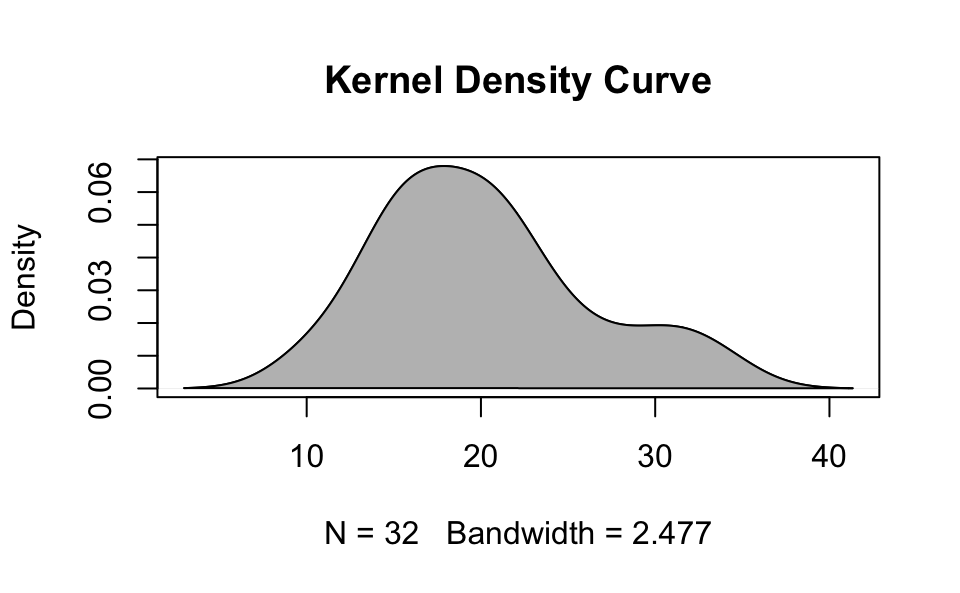
\includegraphics[width=0.7\linewidth,height=0.8\textheight]{R-coding-basics_files/figure-latex/polygons-1} \end{center}

\hypertarget{drawing-text}{%
\subsubsection*{Drawing Text}\label{drawing-text}}
\addcontentsline{toc}{subsubsection}{Drawing Text}

\begin{Shaded}
\begin{Highlighting}[]
\FunctionTok{plot}\NormalTok{(}\FloatTok{0.5}\NormalTok{, }\FloatTok{0.5}\NormalTok{, }\AttributeTok{xlim =} \FunctionTok{c}\NormalTok{(}\DecValTok{0}\NormalTok{, }\DecValTok{1}\NormalTok{), }\AttributeTok{ylim =} \FunctionTok{c}\NormalTok{(}\DecValTok{0}\NormalTok{, }\DecValTok{1}\NormalTok{), }\AttributeTok{type =} \StringTok{\textquotesingle{}n\textquotesingle{}}\NormalTok{)}
\FunctionTok{abline}\NormalTok{(}\AttributeTok{h =} \FunctionTok{c}\NormalTok{(.}\DecValTok{2}\NormalTok{, .}\DecValTok{5}\NormalTok{, .}\DecValTok{8}\NormalTok{),}
       \AttributeTok{v =} \FunctionTok{c}\NormalTok{(.}\DecValTok{5}\NormalTok{, .}\DecValTok{2}\NormalTok{, .}\DecValTok{8}\NormalTok{), }\AttributeTok{col =} \StringTok{"lightgrey"}\NormalTok{)}
\FunctionTok{text}\NormalTok{(}\FloatTok{0.5}\NormalTok{, }\FloatTok{0.5}\NormalTok{, }\StringTok{"srt = 45, adj = c(.5, .5)"}\NormalTok{,}
     \AttributeTok{srt =} \DecValTok{45}\NormalTok{, }\AttributeTok{adj =} \FunctionTok{c}\NormalTok{(.}\DecValTok{5}\NormalTok{, .}\DecValTok{5}\NormalTok{))}
\FunctionTok{text}\NormalTok{(}\FloatTok{0.5}\NormalTok{, }\FloatTok{0.8}\NormalTok{, }\StringTok{"adj = c(0, .5)"}\NormalTok{, }\AttributeTok{adj =} \FunctionTok{c}\NormalTok{(}\DecValTok{0}\NormalTok{, .}\DecValTok{5}\NormalTok{))}
\FunctionTok{text}\NormalTok{(}\FloatTok{0.5}\NormalTok{, }\FloatTok{0.2}\NormalTok{, }\StringTok{"adj = c(1, .5)"}\NormalTok{, }\AttributeTok{adj =} \FunctionTok{c}\NormalTok{(}\DecValTok{1}\NormalTok{, .}\DecValTok{5}\NormalTok{))}
\FunctionTok{text}\NormalTok{(}\FloatTok{0.2}\NormalTok{, }\FloatTok{0.5}\NormalTok{, }\StringTok{"adj = c(1, 1)"}\NormalTok{, }\AttributeTok{adj =} \FunctionTok{c}\NormalTok{(}\DecValTok{1}\NormalTok{, }\DecValTok{1}\NormalTok{))}
\FunctionTok{text}\NormalTok{(}\FloatTok{0.8}\NormalTok{, }\FloatTok{0.5}\NormalTok{, }\StringTok{"adj = c(0, 0)"}\NormalTok{, }\AttributeTok{adj =} \FunctionTok{c}\NormalTok{(}\DecValTok{0}\NormalTok{, }\DecValTok{0}\NormalTok{))}
\end{Highlighting}
\end{Shaded}

\begin{center}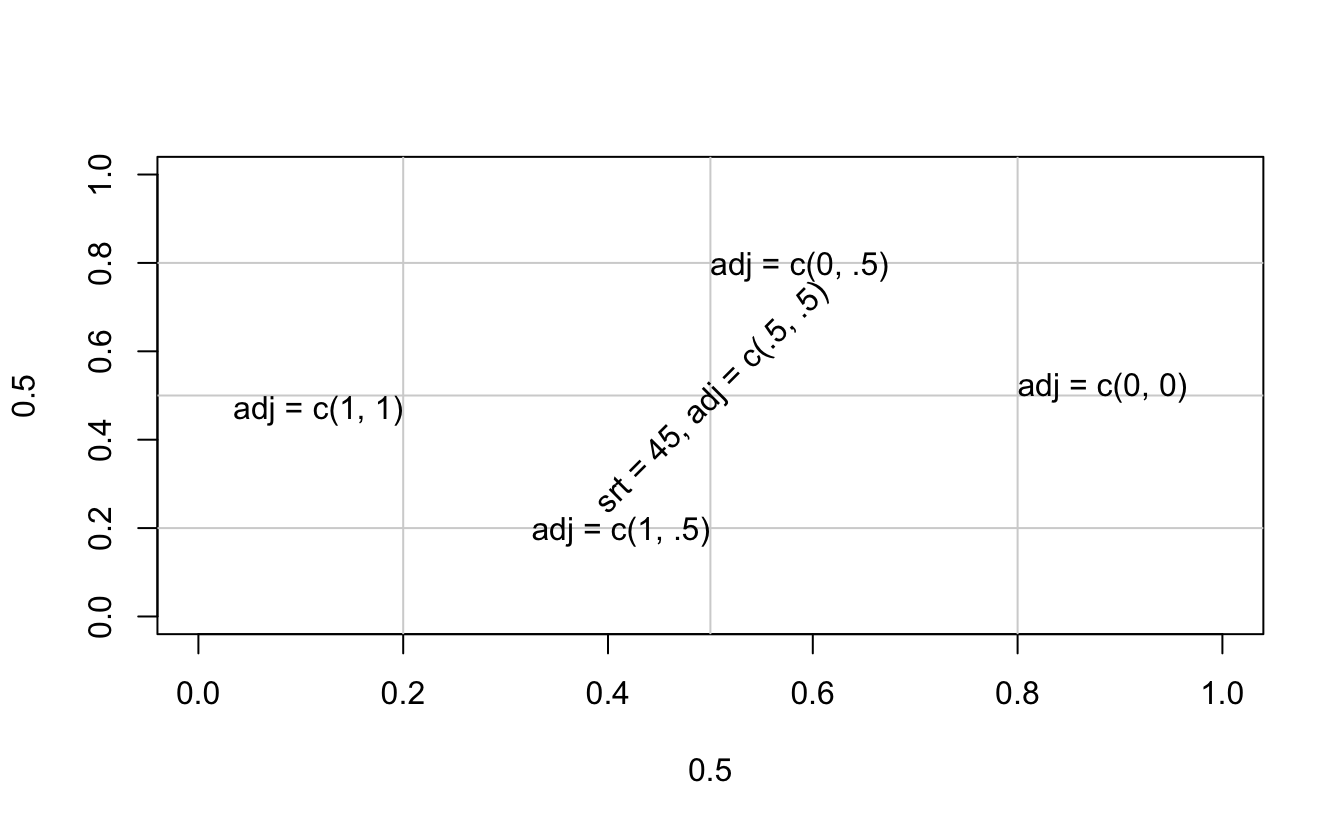
\includegraphics[width=0.7\linewidth,height=0.8\textheight]{R-coding-basics_files/figure-latex/draw_text-1} \end{center}

\hypertarget{graphics2}{%
\chapter{More Base Graphics}\label{graphics2}}

R comes with many functions that let us produce a wide variety of graphics,
plots, diagrams, charts, maps, \ldots{} you name it.

In this chapter we describe the behavior of the \texttt{plot()} method and it
can be used to produce a large number of graphics.

\hypertarget{the-plot-function-1}{%
\section{\texorpdfstring{The \texttt{plot()} function}{The plot() function}}\label{the-plot-function-1}}

\texttt{plot()} is the most important high-level function in traditional graphics

\begin{itemize}
\item
  The first argument to \texttt{plot()} provides the data to plot
\item
  The provided data can take different forms: e.g.~vectors, factors, matrices,
  data frames.
\item
  To be more precise, \texttt{plot()} is a generic function
\item
  You can create your own \texttt{plot()} method function
\end{itemize}

In its basic form, we can use \texttt{plot()} to make graphics of:

\begin{itemize}
\item
  one single variable
\item
  two variables
\item
  multiple variables
\end{itemize}

\hypertarget{one-variable-graphics}{%
\section{One variable graphics}\label{one-variable-graphics}}

High-level graphics of a single variable

\begin{longtable}[]{@{}lll@{}}
\toprule()
Function & Data & Graphic \\
\midrule()
\endhead
\texttt{plot()} & numeric & scatterplot \\
\texttt{plot()} & factor & barplot \\
\texttt{plot()} & 1-D table & barplot \\
\bottomrule()
\end{longtable}

A \texttt{numeric} object can be either a vector or a 1-D array (e.g.~row or column
from a matrix)

\begin{figure}

{\centering 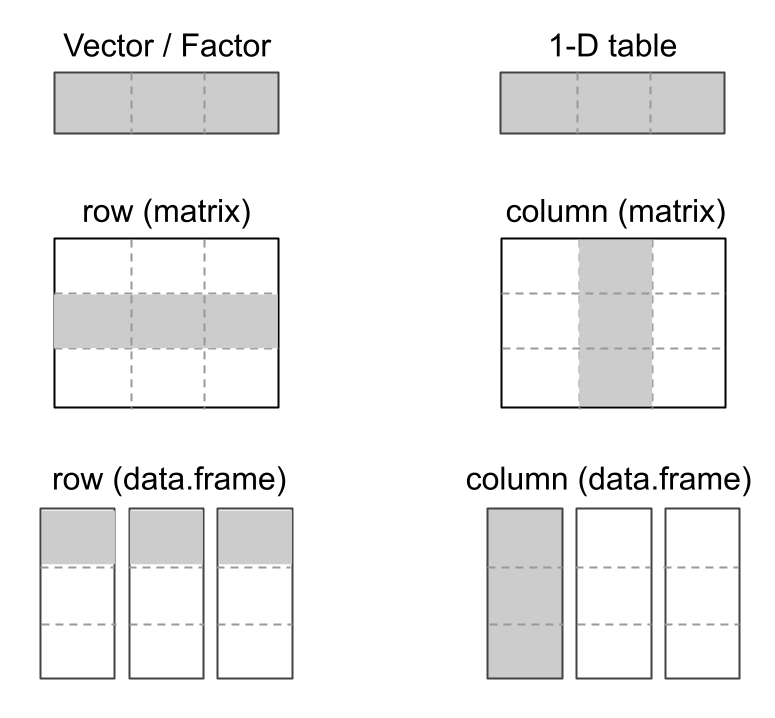
\includegraphics[width=0.5\linewidth]{images/plots/one_variable_objs} 

}

\caption{One-variable objects can take multiple forms.}\label{fig:unnamed-chunk-212}
\end{figure}

Here's an example:

\begin{Shaded}
\begin{Highlighting}[]
\CommentTok{\# plot numeric vector}
\NormalTok{num\_vec }\OtherTok{\textless{}{-}}\NormalTok{ (}\FunctionTok{c}\NormalTok{(}\DecValTok{1}\SpecialCharTok{:}\DecValTok{10}\NormalTok{))}\SpecialCharTok{\^{}}\DecValTok{2}
\FunctionTok{plot}\NormalTok{(num\_vec)}

\CommentTok{\# plot factor}
\FunctionTok{set.seed}\NormalTok{(}\DecValTok{4}\NormalTok{)}
\NormalTok{abc }\OtherTok{\textless{}{-}} \FunctionTok{factor}\NormalTok{(}\FunctionTok{sample}\NormalTok{(}\FunctionTok{c}\NormalTok{(}\StringTok{\textquotesingle{}A\textquotesingle{}}\NormalTok{, }\StringTok{\textquotesingle{}B\textquotesingle{}}\NormalTok{, }\StringTok{\textquotesingle{}C\textquotesingle{}}\NormalTok{), }\DecValTok{20}\NormalTok{, }\AttributeTok{replace =} \ConstantTok{TRUE}\NormalTok{))}
\FunctionTok{plot}\NormalTok{(abc)}

\CommentTok{\# plot 1D{-}table}
\NormalTok{abc\_table }\OtherTok{\textless{}{-}} \FunctionTok{table}\NormalTok{(abc)}
\FunctionTok{plot}\NormalTok{(abc\_table)}
\end{Highlighting}
\end{Shaded}

\begin{center}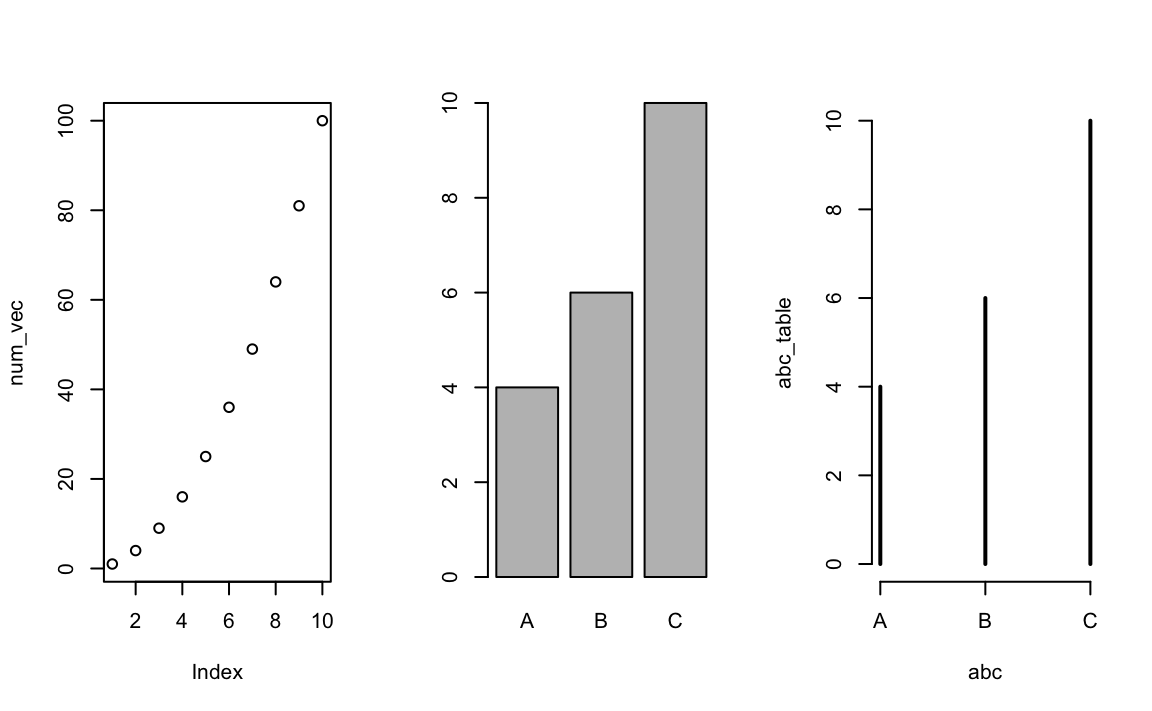
\includegraphics[width=0.9\linewidth]{R-coding-basics_files/figure-latex/plot-single1-1} \end{center}

\hypertarget{more-high-level-graphics-of-a-single-variable}{%
\subsection{More high-level graphics of a single variable}\label{more-high-level-graphics-of-a-single-variable}}

\begin{longtable}[]{@{}lll@{}}
\toprule()
Function & Data & Graphic \\
\midrule()
\endhead
\texttt{barplot()} & numeric & barchart \\
\texttt{pie()} & numeric & piechart \\
\texttt{dotchart()} & numeric & dotplot \\
& & \\
\texttt{boxplot()} & numeric & boxplot \\
\texttt{hist()} & numeric & histogram \\
\texttt{stripchart()} & numeric & 1-D scatterplot \\
\texttt{stem()} & numeric & stem-and-leaf plot \\
\bottomrule()
\end{longtable}

Examples: one signle variable plots

\begin{Shaded}
\begin{Highlighting}[]
\CommentTok{\# barplot numeric vector}
\FunctionTok{barplot}\NormalTok{(num\_vec)}

\CommentTok{\# pie chart}
\FunctionTok{pie}\NormalTok{(}\DecValTok{1}\SpecialCharTok{:}\DecValTok{3}\NormalTok{)}

\CommentTok{\# dot plot}
\FunctionTok{dotchart}\NormalTok{(num\_vec)}
\end{Highlighting}
\end{Shaded}

\begin{center}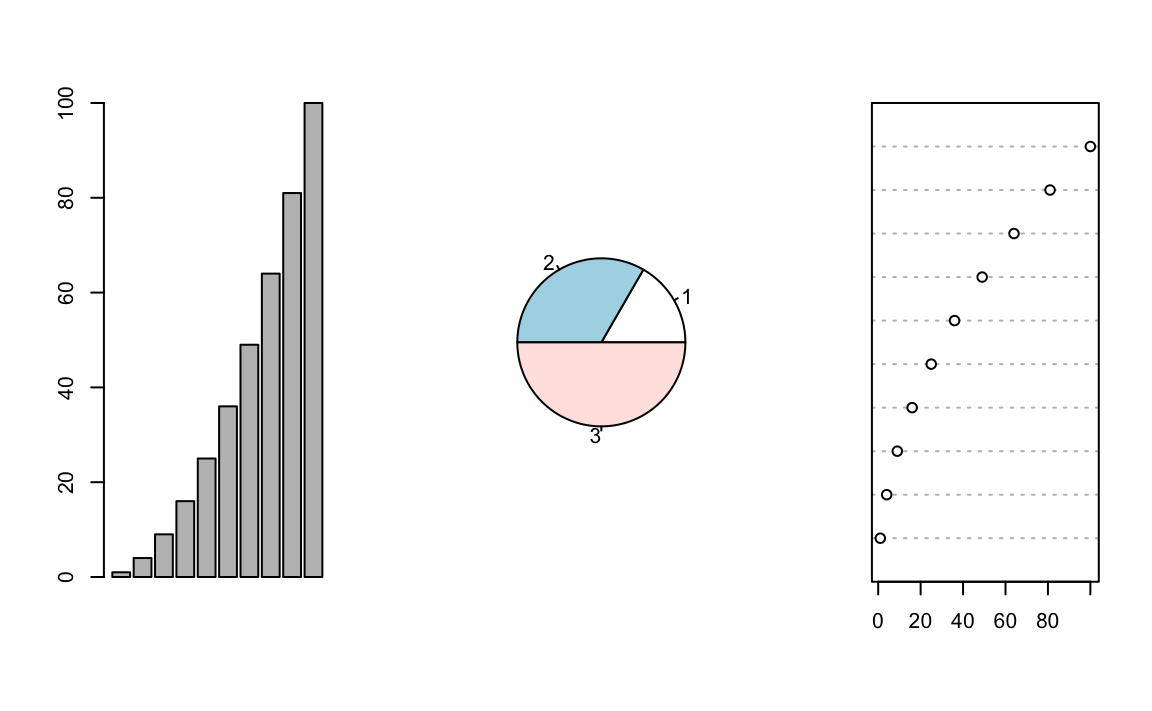
\includegraphics[width=0.9\linewidth]{R-coding-basics_files/figure-latex/plot-single2-1} \end{center}

Examples: one single variable plots

\begin{Shaded}
\begin{Highlighting}[]
\CommentTok{\# barplot numeric vector}
\FunctionTok{boxplot}\NormalTok{(num\_vec)}

\CommentTok{\# pie chart}
\FunctionTok{hist}\NormalTok{(num\_vec)}

\CommentTok{\# dot plot}
\FunctionTok{stripchart}\NormalTok{(num\_vec)}
\end{Highlighting}
\end{Shaded}

\begin{center}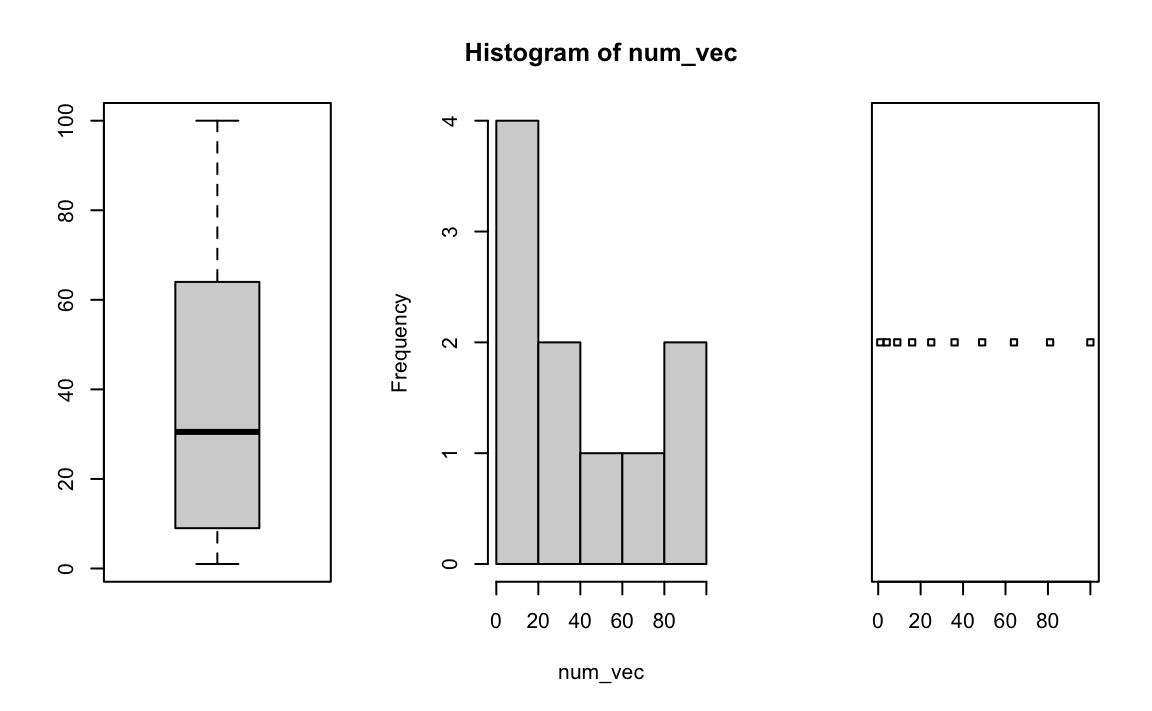
\includegraphics[width=0.9\linewidth]{R-coding-basics_files/figure-latex/plot-single3-1} \end{center}

\hypertarget{plots-of-two-variables}{%
\section{Plots of Two Variables}\label{plots-of-two-variables}}

\begin{longtable}[]{@{}lll@{}}
\toprule()
Function & Data & Graphic \\
\midrule()
\endhead
\texttt{plot()} & numeric & scatterplot \\
\texttt{plot()} & numeric & stripcharts \\
\texttt{plot()} & factor & boxplots \\
\texttt{plot()} & factor & spineplot \\
\texttt{plot()} & 2-column numeric matrix & scatterplot \\
\texttt{plot()} & 2-column numeric data.frame & scatterplot \\
\texttt{plot()} & 2-D table & mosaicplot \\
\bottomrule()
\end{longtable}

A \texttt{numeric} object can be either a vector or a 1-D array (e.g.~row or column
from a matrix)

\begin{figure}

{\centering 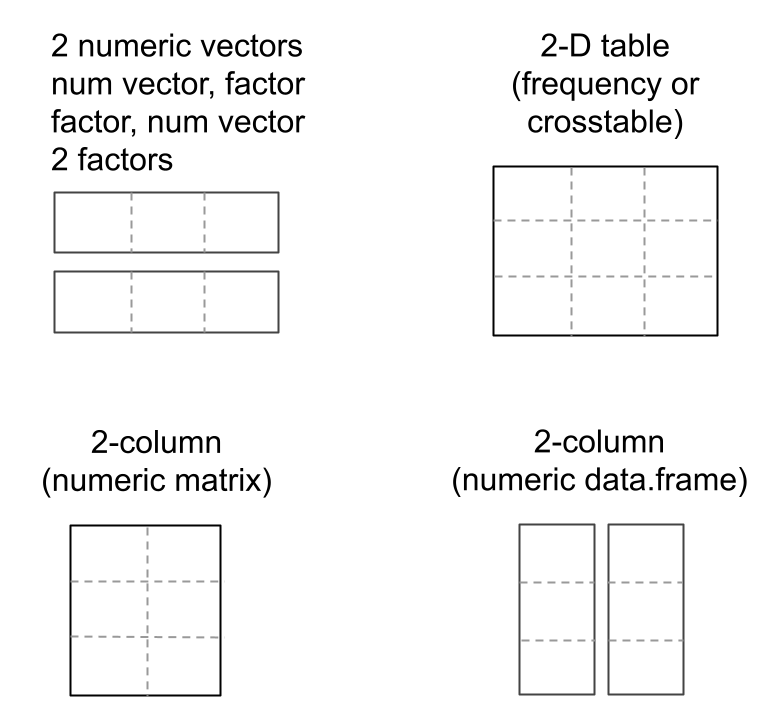
\includegraphics[width=0.6\linewidth]{images/plots/two_variable_objs} 

}

\caption{One-variable objects can take multiple forms.}\label{fig:unnamed-chunk-213}
\end{figure}

Here's an example:

\begin{Shaded}
\begin{Highlighting}[]
\CommentTok{\# plot numeric, numeric}
\FunctionTok{plot}\NormalTok{(iris}\SpecialCharTok{$}\NormalTok{Petal.Length, iris}\SpecialCharTok{$}\NormalTok{Sepal.Length)}

\CommentTok{\# plot numeric, factor}
\FunctionTok{plot}\NormalTok{(iris}\SpecialCharTok{$}\NormalTok{Petal.Length, iris}\SpecialCharTok{$}\NormalTok{Species)}

\CommentTok{\# plot factor, numeric}
\FunctionTok{plot}\NormalTok{(iris}\SpecialCharTok{$}\NormalTok{Species, iris}\SpecialCharTok{$}\NormalTok{Petal.Length)}

\CommentTok{\# plot factor, factor}
\FunctionTok{plot}\NormalTok{(iris}\SpecialCharTok{$}\NormalTok{Species, iris}\SpecialCharTok{$}\NormalTok{Species)}
\end{Highlighting}
\end{Shaded}

\begin{center}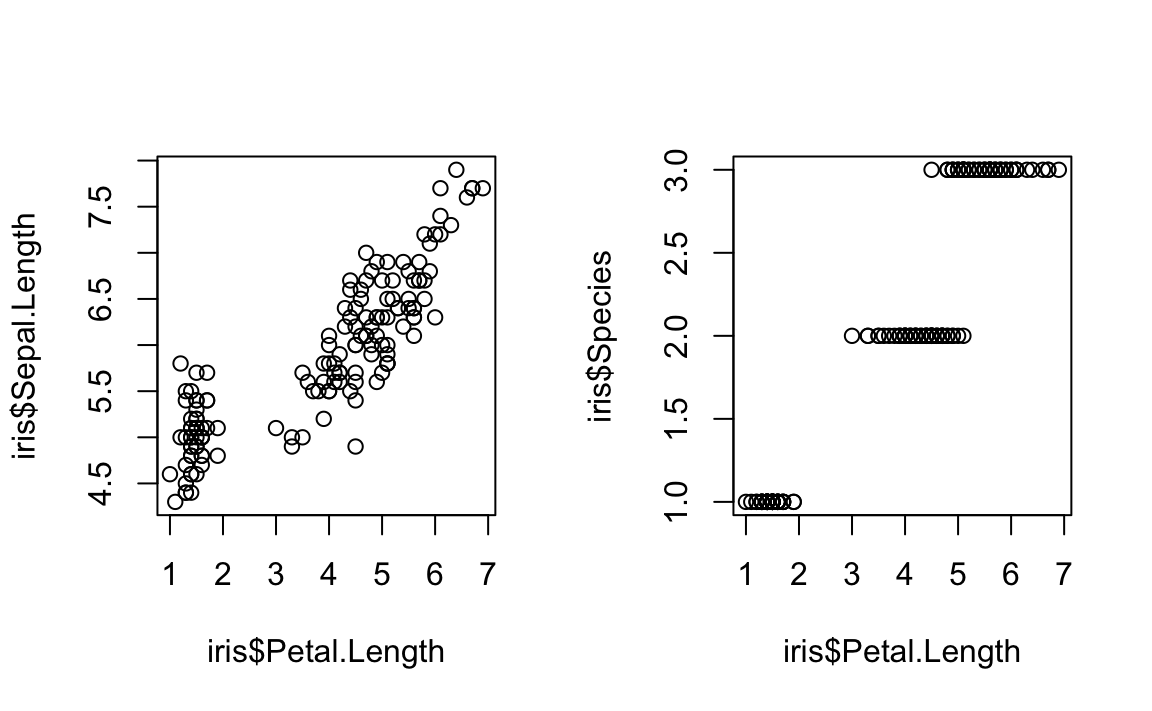
\includegraphics[width=0.85\linewidth]{R-coding-basics_files/figure-latex/unnamed-chunk-214-1} \end{center}

\begin{center}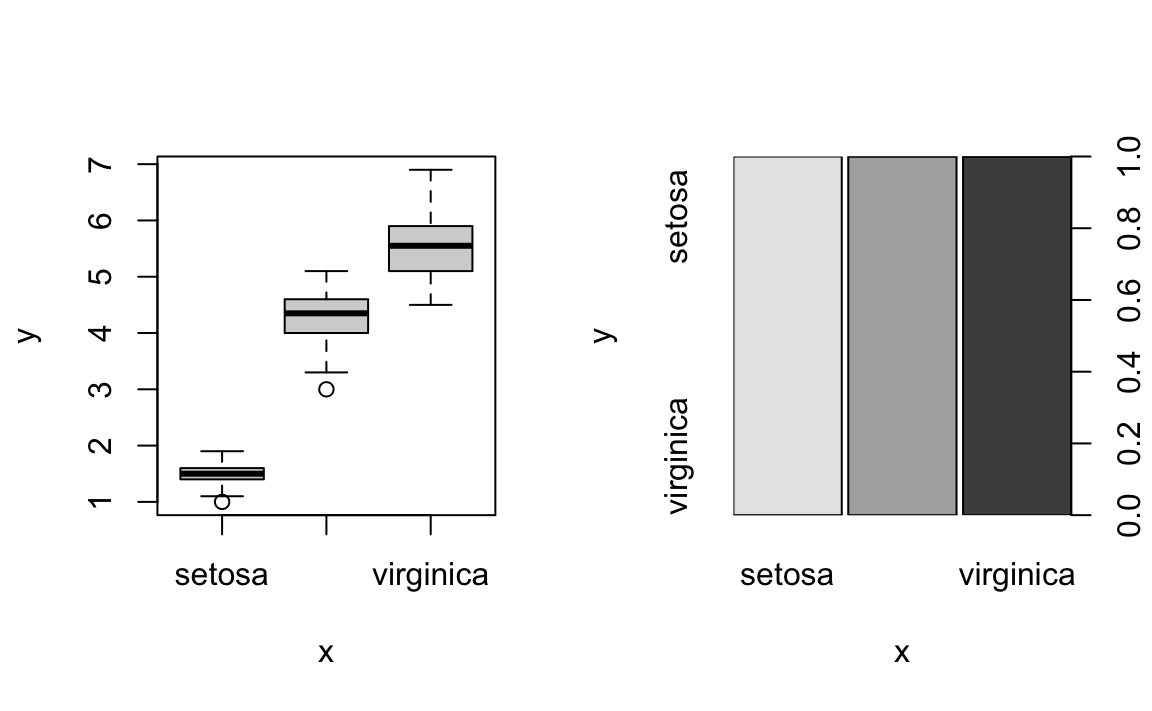
\includegraphics[width=0.85\linewidth]{R-coding-basics_files/figure-latex/unnamed-chunk-215-1} \end{center}

\hypertarget{example-plots-of-two-variables}{%
\subsection{Example: Plots of two variables}\label{example-plots-of-two-variables}}

\begin{Shaded}
\begin{Highlighting}[]
\CommentTok{\# some fake data}
\FunctionTok{set.seed}\NormalTok{(}\DecValTok{1}\NormalTok{)}

\CommentTok{\# hair color}
\NormalTok{hair }\OtherTok{\textless{}{-}} \FunctionTok{factor}\NormalTok{(}
  \FunctionTok{sample}\NormalTok{(}\FunctionTok{c}\NormalTok{(}\StringTok{\textquotesingle{}blond\textquotesingle{}}\NormalTok{, }\StringTok{\textquotesingle{}black\textquotesingle{}}\NormalTok{, }\StringTok{\textquotesingle{}brown\textquotesingle{}}\NormalTok{), }\DecValTok{100}\NormalTok{, }\AttributeTok{replace =} \ConstantTok{TRUE}\NormalTok{))}

\CommentTok{\# eye color}
\NormalTok{eye }\OtherTok{\textless{}{-}} \FunctionTok{factor}\NormalTok{(}
  \FunctionTok{sample}\NormalTok{(}\FunctionTok{c}\NormalTok{(}\StringTok{\textquotesingle{}blue\textquotesingle{}}\NormalTok{, }\StringTok{\textquotesingle{}brown\textquotesingle{}}\NormalTok{, }\StringTok{\textquotesingle{}green\textquotesingle{}}\NormalTok{), }\DecValTok{100}\NormalTok{, }\AttributeTok{replace =} \ConstantTok{TRUE}\NormalTok{))}
\end{Highlighting}
\end{Shaded}

\begin{Shaded}
\begin{Highlighting}[]
\CommentTok{\# plot factor, factor}
\FunctionTok{plot}\NormalTok{(hair, eye)}
\end{Highlighting}
\end{Shaded}

\begin{center}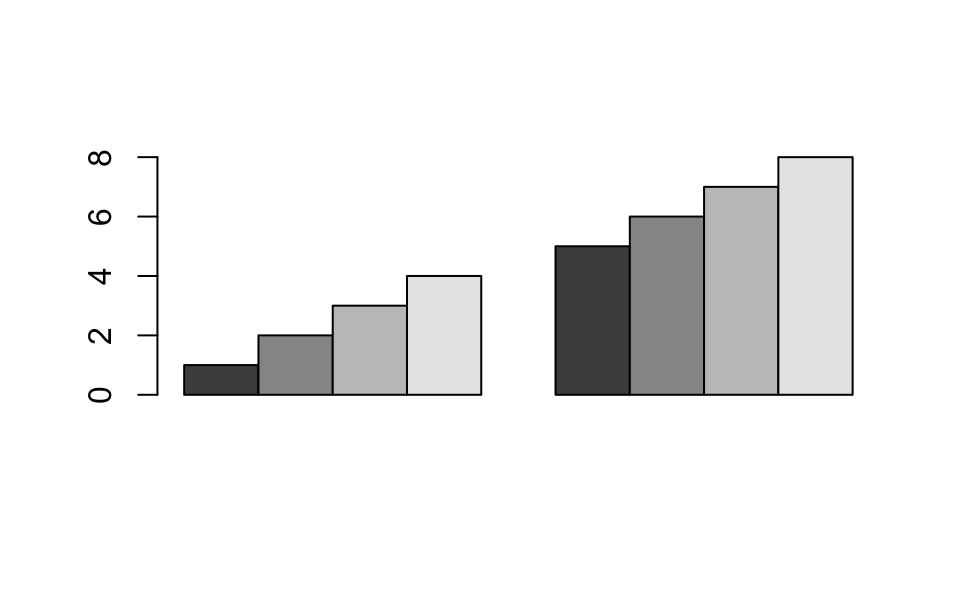
\includegraphics[width=0.8\linewidth]{R-coding-basics_files/figure-latex/unnamed-chunk-217-1} \end{center}

\hypertarget{more-high-level-graphics-of-two-variables}{%
\subsection{More high-level graphics of two variables}\label{more-high-level-graphics-of-two-variables}}

\begin{longtable}[]{@{}lll@{}}
\toprule()
Function & Data & Graphic \\
\midrule()
\endhead
\texttt{sunflowerplot()} & numeric, numeric & sunflower scatterplot \\
\texttt{smoothScatter()} & numeric, numeric & smooth scatterplot \\
\texttt{boxplot()} & list of numeric & boxplots \\
\texttt{barplot()} & matrix & stacked barplot \\
\texttt{dotchart()} & matrix & dotplot \\
\texttt{stripchart()} & list of numeric & stripcharts \\
\texttt{spineplot()} & numeric, factor & spinogram \\
\texttt{cdplot()} & numeric, factor & conditional density plot \\
\texttt{fourfoldplot()} & 2x2 table & fourfold display \\
\texttt{assocplot()} & 2-D table & association plot \\
\texttt{mosaicplot()} & 2-D table & mosaicplot \\
\bottomrule()
\end{longtable}

\hypertarget{sunflower-plot}{%
\subsubsection*{Sunflower plot}\label{sunflower-plot}}
\addcontentsline{toc}{subsubsection}{Sunflower plot}

\begin{Shaded}
\begin{Highlighting}[]
\CommentTok{\# sunflower plot (numeric, numeric)}
\FunctionTok{sunflowerplot}\NormalTok{(iris}\SpecialCharTok{$}\NormalTok{Petal.Length, iris}\SpecialCharTok{$}\NormalTok{Sepal.Length)}
\end{Highlighting}
\end{Shaded}

\begin{center}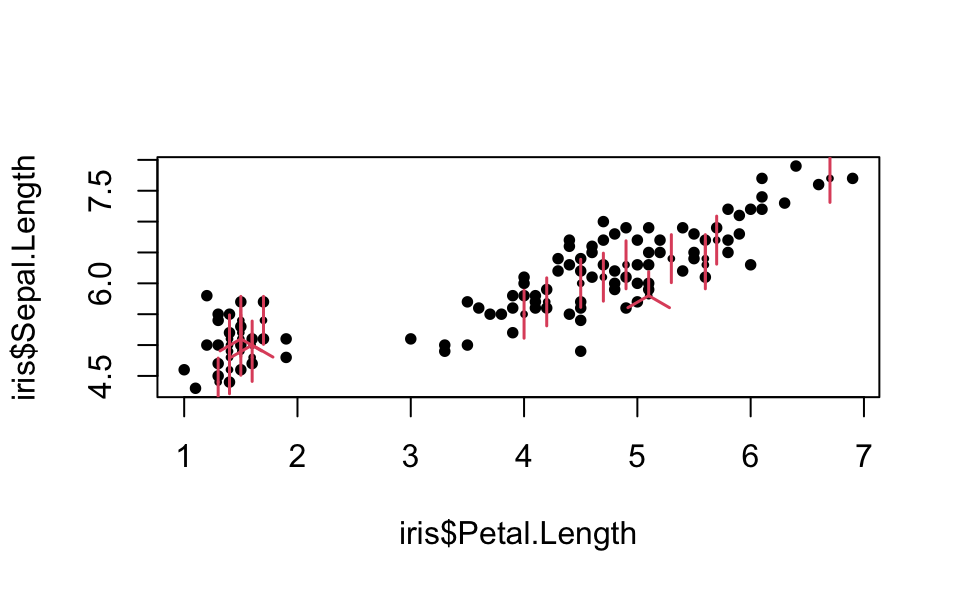
\includegraphics[width=0.75\linewidth]{R-coding-basics_files/figure-latex/unnamed-chunk-218-1} \end{center}

\hypertarget{smooth-scatter-plot}{%
\subsubsection*{Smooth scatter plot}\label{smooth-scatter-plot}}
\addcontentsline{toc}{subsubsection}{Smooth scatter plot}

\begin{Shaded}
\begin{Highlighting}[]
\CommentTok{\# smooth scatter plot (numeric, numeric)}
\FunctionTok{smoothScatter}\NormalTok{(iris}\SpecialCharTok{$}\NormalTok{Petal.Length, iris}\SpecialCharTok{$}\NormalTok{Sepal.Length)}
\end{Highlighting}
\end{Shaded}

\begin{center}\includegraphics[width=0.75\linewidth]{R-coding-basics_files/figure-latex/unnamed-chunk-219-1} \end{center}

\hypertarget{boxplots}{%
\subsubsection*{Boxplots}\label{boxplots}}
\addcontentsline{toc}{subsubsection}{Boxplots}

\begin{Shaded}
\begin{Highlighting}[]
\CommentTok{\# boxplots (numeric, numeric)}
\FunctionTok{boxplot}\NormalTok{(iris}\SpecialCharTok{$}\NormalTok{Petal.Length, iris}\SpecialCharTok{$}\NormalTok{Sepal.Length)}
\end{Highlighting}
\end{Shaded}

\begin{center}\includegraphics[width=0.75\linewidth]{R-coding-basics_files/figure-latex/unnamed-chunk-220-1} \end{center}

\hypertarget{barplot}{%
\subsubsection*{Barplot}\label{barplot}}
\addcontentsline{toc}{subsubsection}{Barplot}

\begin{Shaded}
\begin{Highlighting}[]
\NormalTok{m }\OtherTok{\textless{}{-}} \FunctionTok{matrix}\NormalTok{(}\DecValTok{1}\SpecialCharTok{:}\DecValTok{8}\NormalTok{, }\DecValTok{4}\NormalTok{, }\DecValTok{2}\NormalTok{)}
\CommentTok{\# barplot (numeric matrix)}
\FunctionTok{barplot}\NormalTok{(m, }\AttributeTok{beside =} \ConstantTok{TRUE}\NormalTok{)}
\end{Highlighting}
\end{Shaded}

\begin{center}\includegraphics[width=0.75\linewidth]{R-coding-basics_files/figure-latex/unnamed-chunk-221-1} \end{center}

\hypertarget{conditional-density-plot}{%
\subsubsection*{Conditional Density Plot}\label{conditional-density-plot}}
\addcontentsline{toc}{subsubsection}{Conditional Density Plot}

\begin{Shaded}
\begin{Highlighting}[]
\CommentTok{\# conditional density plot (numeric, factor)}
\FunctionTok{cdplot}\NormalTok{(iris}\SpecialCharTok{$}\NormalTok{Petal.Length, iris}\SpecialCharTok{$}\NormalTok{Species)}
\end{Highlighting}
\end{Shaded}

\begin{center}\includegraphics[width=0.75\linewidth]{R-coding-basics_files/figure-latex/unnamed-chunk-222-1} \end{center}

\hypertarget{graphics3}{%
\chapter{Plots from Scratch}\label{graphics3}}

In this chapter we describe one of my favorite graphing approaches to create
what I like to call \emph{plots from scratch}. That is, making a graph in a way
that we have full control of all the nitty-gritty details of a plot.

\hypertarget{making-a-graphic-from-scratch}{%
\section{Making a graphic from scratch}\label{making-a-graphic-from-scratch}}

In addition to using \texttt{plot()}, possibly calling one or more low-level
functions, you should know that it is also possible to create a plot from
scratch. Although this procedure is less documented, it is extremely flexible
and powerful. The general recipe to create a plot with this approach is as
follows:

\begin{itemize}
\item
  call \texttt{plot.new()} to start a new plot frame
\item
  call \texttt{plot.window()} to define coordinates
\item
  then call low-level functions:
\item
  typical options involve \texttt{axis()}
\item
  then \texttt{title()} (title, subtitle)
\item
  after that call other function: e.g.~\texttt{points()}, \texttt{lines()}, etc
\end{itemize}

\begin{Shaded}
\begin{Highlighting}[]
\FunctionTok{plot.new}\NormalTok{()}
\FunctionTok{plot.window}\NormalTok{(}\AttributeTok{xlim =} \FunctionTok{c}\NormalTok{(}\DecValTok{0}\NormalTok{, }\DecValTok{10}\NormalTok{), }\AttributeTok{ylim =} \FunctionTok{c}\NormalTok{(}\SpecialCharTok{{-}}\DecValTok{2}\NormalTok{, }\DecValTok{4}\NormalTok{), }\AttributeTok{xaxs =} \StringTok{"i"}\NormalTok{)}
\FunctionTok{axis}\NormalTok{(}\AttributeTok{side =} \DecValTok{1}\NormalTok{, }\AttributeTok{col.axis =} \StringTok{"grey30"}\NormalTok{)}
\FunctionTok{axis}\NormalTok{(}\AttributeTok{side =} \DecValTok{2}\NormalTok{, }\AttributeTok{col.axis =} \StringTok{"grey30"}\NormalTok{, }\AttributeTok{las =} \DecValTok{1}\NormalTok{)}
\FunctionTok{title}\NormalTok{(}\AttributeTok{main =} \StringTok{"Main Title"}\NormalTok{,}
      \AttributeTok{col.main =} \StringTok{"tomato"}\NormalTok{,}
      \AttributeTok{sub =} \StringTok{"Plot Subtitle"}\NormalTok{,}
      \AttributeTok{col.sub =} \StringTok{"orange"}\NormalTok{,}
      \AttributeTok{xlab =} \StringTok{"x{-}axis"}\NormalTok{, }
      \AttributeTok{ylab =} \StringTok{"y{-}axis"}\NormalTok{,}
      \AttributeTok{col.lab =} \StringTok{"blue"}\NormalTok{, }
      \AttributeTok{font.lab =} \DecValTok{3}\NormalTok{)}
\FunctionTok{box}\NormalTok{(}\StringTok{"figure"}\NormalTok{, }\AttributeTok{col =} \StringTok{"grey90"}\NormalTok{)}
\end{Highlighting}
\end{Shaded}

\begin{center}\includegraphics[width=0.7\linewidth,height=0.8\textheight]{R-coding-basics_files/figure-latex/bare_plot-1} \end{center}

Here's another example:

\begin{Shaded}
\begin{Highlighting}[]
\FunctionTok{set.seed}\NormalTok{(}\DecValTok{5}\NormalTok{)}
\NormalTok{x }\OtherTok{\textless{}{-}} \FunctionTok{rnorm}\NormalTok{(}\DecValTok{200}\NormalTok{)}
\NormalTok{y }\OtherTok{\textless{}{-}}\NormalTok{ x }\SpecialCharTok{+} \FunctionTok{rnorm}\NormalTok{(}\DecValTok{200}\NormalTok{)}

\FunctionTok{plot.new}\NormalTok{()}
\FunctionTok{plot.window}\NormalTok{(}\AttributeTok{xlim =} \FunctionTok{c}\NormalTok{(}\SpecialCharTok{{-}}\FloatTok{4.5}\NormalTok{, }\FloatTok{4.5}\NormalTok{), }\AttributeTok{xaxs =} \StringTok{"i"}\NormalTok{, }
            \AttributeTok{ylim =} \FunctionTok{c}\NormalTok{(}\SpecialCharTok{{-}}\FloatTok{4.5}\NormalTok{, }\FloatTok{4.5}\NormalTok{), }\AttributeTok{yaxs =} \StringTok{"i"}\NormalTok{)}
\NormalTok{z }\OtherTok{\textless{}{-}} \FunctionTok{lm}\NormalTok{(y }\SpecialCharTok{\textasciitilde{}}\NormalTok{ x)}
\FunctionTok{abline}\NormalTok{(}\AttributeTok{h =} \SpecialCharTok{{-}}\DecValTok{4}\SpecialCharTok{:}\DecValTok{4}\NormalTok{, }\AttributeTok{v =} \SpecialCharTok{{-}}\DecValTok{4}\SpecialCharTok{:}\DecValTok{4}\NormalTok{, }\AttributeTok{col =} \StringTok{"lightgrey"}\NormalTok{)}
\FunctionTok{abline}\NormalTok{(}\AttributeTok{a =} \FunctionTok{coef}\NormalTok{(z)[}\DecValTok{1}\NormalTok{], }\AttributeTok{b =} \FunctionTok{coef}\NormalTok{(z)[}\DecValTok{2}\NormalTok{], }\AttributeTok{lwd =} \DecValTok{2}\NormalTok{, }\AttributeTok{col =} \StringTok{"red"}\NormalTok{)}
\FunctionTok{points}\NormalTok{(x, y)}
\FunctionTok{axis}\NormalTok{(}\AttributeTok{side =} \DecValTok{1}\NormalTok{)}
\FunctionTok{axis}\NormalTok{(}\AttributeTok{side =} \DecValTok{2}\NormalTok{, }\AttributeTok{las =} \DecValTok{1}\NormalTok{)}
\FunctionTok{box}\NormalTok{()}
\FunctionTok{title}\NormalTok{(}\AttributeTok{main =} \StringTok{"A Fitted Regression Line"}\NormalTok{)}
\end{Highlighting}
\end{Shaded}

\begin{center}\includegraphics[width=0.7\linewidth,height=0.8\textheight]{R-coding-basics_files/figure-latex/ablines-1} \end{center}

\hypertarget{how-does-it-work}{%
\subsection{How does it work}\label{how-does-it-work}}

You start a new plot with \texttt{plot.new()}

\begin{itemize}
\item
  \texttt{plot.new()} opens a new (empty) plot frame
\item
  \texttt{plot.new()} chooses a default plotting region
\end{itemize}

After starting with \texttt{plot.new()}, use \texttt{plot.window()} to set up the coordinate
system for the plotting frame

\begin{Shaded}
\begin{Highlighting}[]
\CommentTok{\# axis limits (0,1)x(0,1)}
\FunctionTok{plot.window}\NormalTok{(}\AttributeTok{xlim =} \FunctionTok{c}\NormalTok{(}\DecValTok{0}\NormalTok{, }\DecValTok{1}\NormalTok{), }\AttributeTok{ylim =} \FunctionTok{c}\NormalTok{(}\DecValTok{0}\NormalTok{, }\DecValTok{1}\NormalTok{))}
\end{Highlighting}
\end{Shaded}

By default \texttt{plot.window()} produces axis limits which are expanded by 6\%
over those actually specified.

The default limits expansion can be turned-off by specifying \texttt{xaxs\ =\ "i"}
and/or \texttt{yaxs\ =\ "i"}

\begin{Shaded}
\begin{Highlighting}[]
\FunctionTok{plot.window}\NormalTok{(xlim, ylim, }\AttributeTok{xaxs =} \StringTok{"i"}\NormalTok{)}
\end{Highlighting}
\end{Shaded}

\hypertarget{aspect-ratio-control}{%
\subsubsection*{Aspect Ratio Control}\label{aspect-ratio-control}}
\addcontentsline{toc}{subsubsection}{Aspect Ratio Control}

Another important argument is \texttt{asp}, which allows us to specify the
\textbf{aspect ratio}

\begin{Shaded}
\begin{Highlighting}[]
\FunctionTok{plot.window}\NormalTok{(xlim, ylim, }\AttributeTok{xaxs =} \StringTok{"i"}\NormalTok{, }\AttributeTok{asp =} \DecValTok{1}\NormalTok{)}
\end{Highlighting}
\end{Shaded}

\texttt{asp\ =\ 1} means that unit steps in the \texttt{x} and \texttt{y} directions produce equal
distances in the \texttt{x} and \texttt{y} directions on the plot.

(Important for avoiding distortion of circles that look like ellipses)

\hypertarget{drawing-axes}{%
\subsubsection*{Drawing Axes}\label{drawing-axes}}
\addcontentsline{toc}{subsubsection}{Drawing Axes}

The \texttt{axis()} function can be used to draw axes at any of the four sides of a plot.

\begin{itemize}
\item
  \texttt{side\ =\ 1} below the graph
\item
  \texttt{side\ =\ 2} to the left of the graph
\item
  \texttt{side\ =\ 3} above the graph
\item
  \texttt{side\ =\ 4} to the right of the graph
\end{itemize}

Axes can be customized via several arguments (see \texttt{?axis})

\begin{itemize}
\item
  location of tick-marks
\item
  labels of axis
\item
  colors
\item
  sizes
\item
  text fonts
\item
  text orientation
\end{itemize}

\hypertarget{plot-annotatiosn}{%
\subsubsection*{Plot Annotatiosn}\label{plot-annotatiosn}}
\addcontentsline{toc}{subsubsection}{Plot Annotatiosn}

The function \texttt{title()} allows us to include labels in the margins

\begin{itemize}
\item
  \texttt{main} main title above the graph
\item
  \texttt{sub} subtitle below the graph
\item
  \texttt{xlab} label for the x-axis
\item
  \texttt{ylab} label for the y-axis
\end{itemize}

The annotations can be customized with additional arguments for the fonts,
colors, and size (expansion)

\begin{itemize}
\item
  \texttt{font.main}, \texttt{col.main}, \texttt{cex.main}
\item
  \texttt{font.sub}, \texttt{col.sub}, \texttt{cex.sub}
\item
  \texttt{font.lab}, \texttt{col.lab}, \texttt{cex.lab}
\end{itemize}

\hypertarget{drawing-arrows}{%
\subsection{Drawing Arrows}\label{drawing-arrows}}

\begin{Shaded}
\begin{Highlighting}[]
\FunctionTok{plot.new}\NormalTok{()}
\FunctionTok{plot.window}\NormalTok{(}\AttributeTok{xlim =} \FunctionTok{c}\NormalTok{(}\DecValTok{0}\NormalTok{, }\DecValTok{1}\NormalTok{), }\AttributeTok{ylim =} \FunctionTok{c}\NormalTok{(}\DecValTok{0}\NormalTok{, }\DecValTok{1}\NormalTok{))}
\FunctionTok{arrows}\NormalTok{(}\FloatTok{0.05}\NormalTok{, }\FloatTok{0.075}\NormalTok{, }\FloatTok{0.45}\NormalTok{, }\FloatTok{0.9}\NormalTok{, }\AttributeTok{code =} \DecValTok{1}\NormalTok{)}
\FunctionTok{arrows}\NormalTok{(}\FloatTok{0.55}\NormalTok{, }\FloatTok{0.9}\NormalTok{, }\FloatTok{0.95}\NormalTok{, }\FloatTok{0.075}\NormalTok{, }\AttributeTok{code =} \DecValTok{2}\NormalTok{)}
\FunctionTok{arrows}\NormalTok{(}\FloatTok{0.1}\NormalTok{, }\DecValTok{0}\NormalTok{, }\FloatTok{0.9}\NormalTok{, }\DecValTok{0}\NormalTok{, }\AttributeTok{code =} \DecValTok{3}\NormalTok{)}
\FunctionTok{text}\NormalTok{(}\FloatTok{0.5}\NormalTok{, }\DecValTok{1}\NormalTok{, }\StringTok{"A"}\NormalTok{, }\AttributeTok{cex =} \FloatTok{1.5}\NormalTok{)}
\FunctionTok{text}\NormalTok{(}\DecValTok{0}\NormalTok{, }\DecValTok{0}\NormalTok{, }\StringTok{"B"}\NormalTok{, }\AttributeTok{cex =} \FloatTok{1.5}\NormalTok{)}
\FunctionTok{text}\NormalTok{(}\DecValTok{1}\NormalTok{, }\DecValTok{0}\NormalTok{, }\StringTok{"C"}\NormalTok{, }\AttributeTok{cex =} \FloatTok{1.5}\NormalTok{)}
\end{Highlighting}
\end{Shaded}

\begin{center}\includegraphics[width=0.7\linewidth,height=0.7\textheight]{R-coding-basics_files/figure-latex/arrows-1} \end{center}

\hypertarget{drawing-rectangles}{%
\subsection{Drawing Rectangles}\label{drawing-rectangles}}

Rectangles can be drawn with the function:

\begin{verbatim}
rect(x0, y0, x1, y1, col = str, border = str)
\end{verbatim}

\begin{itemize}
\item
  \texttt{x0,\ y0,\ x1,\ y1} give the coordinates of diagonally opposite corners of the
  rectangles/
\item
  \texttt{col} specifies the color of the interior.
\item
  \texttt{border} specifies the color of the border/
\end{itemize}

\begin{Shaded}
\begin{Highlighting}[]
\CommentTok{\# barplot "manually" constructed}
\FunctionTok{plot.new}\NormalTok{()}
\FunctionTok{plot.window}\NormalTok{(}\AttributeTok{xlim =} \FunctionTok{c}\NormalTok{(}\DecValTok{0}\NormalTok{, }\DecValTok{5}\NormalTok{), }\AttributeTok{ylim =} \FunctionTok{c}\NormalTok{(}\DecValTok{0}\NormalTok{, }\DecValTok{10}\NormalTok{))}
\FunctionTok{rect}\NormalTok{(}\DecValTok{0}\SpecialCharTok{:}\DecValTok{4}\NormalTok{, }\DecValTok{0}\NormalTok{, }\DecValTok{1}\SpecialCharTok{:}\DecValTok{5}\NormalTok{, }\FunctionTok{c}\NormalTok{(}\DecValTok{7}\NormalTok{, }\DecValTok{8}\NormalTok{, }\DecValTok{4}\NormalTok{, }\DecValTok{3}\NormalTok{), }
     \AttributeTok{col =} \StringTok{"turquoise"}\NormalTok{,}
     \AttributeTok{border =} \StringTok{"white"}\NormalTok{)}
\FunctionTok{axis}\NormalTok{(}\DecValTok{1}\NormalTok{)}
\FunctionTok{axis}\NormalTok{(}\DecValTok{2}\NormalTok{, }\AttributeTok{las =} \DecValTok{1}\NormalTok{)}
\end{Highlighting}
\end{Shaded}

\begin{center}\includegraphics[width=0.6\linewidth,height=0.7\textheight]{R-coding-basics_files/figure-latex/rectangles-1} \end{center}

\hypertarget{part-programming-basics}{%
\part{Programming Basics}\label{part-programming-basics}}

\hypertarget{functions1}{%
\chapter{Intro to Functions}\label{functions1}}

R comes with many functions and packages that let us perform a wide variety
of tasks, and so far we've been using a number of them. In fact, most of the
things we do in R is by calling some function. Sometimes, however, there is no
function to do what we want to achieve. When this is the case, we may very
well want to write our own functions.

In this chapter we'll describe how to start writing small and simple functions.
We are going to start covering the ``tip of the iceberg'', and in the following
chapters we will continue discussing more aspects about writing functions, and
describing how R works when you invoke (call) a function.

\hypertarget{motivation-3}{%
\section{Motivation}\label{motivation-3}}

We've used the formula of \textbf{future value}, given below, which is useful to
answer questions like: If you deposit \$1000 into a savings account that pays
an annual interest of 2\%, how much will you have at the end of year 10?

\[
\text{FV} = \text{PV} \times (1 + r)^n
\]

\begin{itemize}
\tightlist
\item
  \(\text{FV}\) = future value (how much you'll have)
\item
  \(\text{PV}\) = present value (the initial deposit)
\item
  \(r\) = rate of return (e.g.~annual rate of return)
\item
  \(n\) = number of periods (e.g.~number of years)
\end{itemize}

R has a large number of functions---e.g.~\texttt{sqrt()}, \texttt{log()}, \texttt{mean()},
\texttt{sd()}, \texttt{exp()}, etc---but it does not have a built-in function to compute
future value.

Wouldn't it be nice to have a \texttt{future\_value()} function---or an \texttt{fv()}
function---that you could call in R? Perhaps something like:

\begin{Shaded}
\begin{Highlighting}[]
\FunctionTok{future\_value}\NormalTok{(}\AttributeTok{present =} \DecValTok{1000}\NormalTok{, }\AttributeTok{rate =} \FloatTok{0.02}\NormalTok{, }\AttributeTok{year =} \DecValTok{10}\NormalTok{)}
\end{Highlighting}
\end{Shaded}

Let's create such a function!

\hypertarget{writing-a-simple-function}{%
\section{Writing a Simple Function}\label{writing-a-simple-function}}

This won't always be the case, but in our current example we have a specific
mathematical formula to work with (which makes things a lot easier):

\[
\text{FV} = \text{PV} \times (1 + r)^n
\]

Like other programming languages that can be used for scientific computations,
we can take advantage of the syntax in R to write an expression that is almost
identical to the algebraic formulation:

\begin{Shaded}
\begin{Highlighting}[]
\NormalTok{fv }\OtherTok{=}\NormalTok{ pv }\SpecialCharTok{*}\NormalTok{ (}\DecValTok{1} \SpecialCharTok{+}\NormalTok{ r)}\SpecialCharTok{\^{}}\NormalTok{n}
\end{Highlighting}
\end{Shaded}

We will use this simple line of code as our starting point for creating a
future value function. Here is how to do it ``logically'' step by step.

\hypertarget{step-1-start-with-a-concrete-example}{%
\subsubsection*{Step 1: Start with a concrete example}\label{step-1-start-with-a-concrete-example}}
\addcontentsline{toc}{subsubsection}{Step 1: Start with a concrete example}

You should always start with a \textbf{small and concrete example}, focusing
on writing code that does the job. For example, we could write the following
lines:

\begin{Shaded}
\begin{Highlighting}[]
\CommentTok{\# inputs}
\NormalTok{pv }\OtherTok{=} \DecValTok{1000}
\NormalTok{r }\OtherTok{=} \FloatTok{0.02}
\NormalTok{n }\OtherTok{=} \DecValTok{10}

\CommentTok{\# process}
\NormalTok{fv }\OtherTok{=}\NormalTok{ pv }\SpecialCharTok{*}\NormalTok{ (}\DecValTok{1} \SpecialCharTok{+}\NormalTok{ r)}\SpecialCharTok{\^{}}\NormalTok{n}

\CommentTok{\# output}
\NormalTok{fv}
\SpecialCharTok{\textgreater{}}\NormalTok{ [}\DecValTok{1}\NormalTok{] }\FloatTok{1218.994}
\end{Highlighting}
\end{Shaded}

When I say ``small example'' I mean working with objects containing just a few
values. Here, the objects \texttt{pv}, \texttt{r}, and \texttt{n} are super simple vectors of size 1.
Sometimes, though, you may want to start with less simple---yet small---objects
containing just a couple of values. That's fine too.

Sometimes you may even need to start not just with one, but with a couple of
concrete examples that will help you get a better feeling of what kind of
objects, and operations you need to use.

As you get more experience creating and writing functions, you may want to
start with a ``medium-size'' concrete example. Personally, I don't tend to start
like this. Instead, I like to take baby-steps, and I also like to take my time,
without rushing the coding. You know the old-saying: ``measure twice, cut once.''

An important part of starting with a concrete example is so that you can
identify what the inputs are, what computations or process the inputs will go
through, and what the output should be.

Inputs:

\begin{itemize}
\tightlist
\item
  \texttt{pv}
\item
  \texttt{r}
\item
  \texttt{n}
\end{itemize}

Process:

\begin{itemize}
\tightlist
\item
  \texttt{fv\ =\ pv\ *\ (1\ +\ r)\^{}n}
\end{itemize}

Output:

\begin{itemize}
\tightlist
\item
  \texttt{fv}
\end{itemize}

\hypertarget{step-2-make-your-code-more-generalizable}{%
\subsubsection*{Step 2: Make your code more generalizable}\label{step-2-make-your-code-more-generalizable}}
\addcontentsline{toc}{subsubsection}{Step 2: Make your code more generalizable}

After having one (or a few) concrete example(s), the next step is to make your
code more generalizable, or if you prefer, to make it more abstract (or at
least less concrete).

Instead of working with specific values \texttt{pv}, \texttt{r}, and \texttt{n}, you can give them
a more algebraic spirit. For instance, the code below considers ``open-ended''
inputs without assigning them any values

\begin{Shaded}
\begin{Highlighting}[]
\CommentTok{\# general inputs (could take "any" values)}
\NormalTok{pv}
\NormalTok{r}
\NormalTok{n}

\CommentTok{\# process}
\NormalTok{fv }\OtherTok{=}\NormalTok{ pv }\SpecialCharTok{*}\NormalTok{ (}\DecValTok{1} \SpecialCharTok{+}\NormalTok{ r)}\SpecialCharTok{\^{}}\NormalTok{n}

\CommentTok{\# output}
\NormalTok{fv}
\end{Highlighting}
\end{Shaded}

Obviously this piece of code is very abstract and not intended to be executed
in R; this is just for the sake of conceptual illustration.

\hypertarget{step-3-encapsulate-the-code-into-a-function}{%
\subsubsection*{Step 3: Encapsulate the code into a function}\label{step-3-encapsulate-the-code-into-a-function}}
\addcontentsline{toc}{subsubsection}{Step 3: Encapsulate the code into a function}

The next step is to encapsulate your code as a formal function in R. I will
show you how to do this in two logical substeps, although keep in mind that in
practice you will merge these two substeps into a single one.

The encapsulation process involves placing the ``inputs'' inside the function
\texttt{function()}, separating each input with a comma. Formally speaking, the
inputs of your functions are known as the \textbf{arguments} of the function.

Likewise, the lines of code that correspond to the ``process'' and ``output'' are
what will become the \textbf{body} of the function. Typically, you encapsulate the
code of the body by surrounding it with curly braces \texttt{\{\ \}}

\begin{Shaded}
\begin{Highlighting}[]
\CommentTok{\# encapsulating code into a function}
\ControlFlowTok{function}\NormalTok{(pv, r, n) \{}
\NormalTok{  fv }\OtherTok{=}\NormalTok{ pv }\SpecialCharTok{*}\NormalTok{ (}\DecValTok{1} \SpecialCharTok{+}\NormalTok{ r)}\SpecialCharTok{\^{}}\NormalTok{n}
\NormalTok{  fv}
\NormalTok{\}}
\end{Highlighting}
\end{Shaded}

The other substep typically consists of \textbf{assigning a name} to the code of
your function. For example, you can give it the name \texttt{FV}:

\begin{Shaded}
\begin{Highlighting}[]
\CommentTok{\# future value function}
\NormalTok{FV }\OtherTok{=} \ControlFlowTok{function}\NormalTok{(pv, r, n) \{}
\NormalTok{  fv }\OtherTok{=}\NormalTok{ pv }\SpecialCharTok{*}\NormalTok{ (}\DecValTok{1} \SpecialCharTok{+}\NormalTok{ r)}\SpecialCharTok{\^{}}\NormalTok{n}
\NormalTok{  fv}
\NormalTok{\}}
\end{Highlighting}
\end{Shaded}

In summary:

\begin{itemize}
\item
  the inputs go inside \texttt{function()}, separating each input with a comma
\item
  the processing step and the output are surrounded within curly braces \texttt{\{\ \}}
\item
  you typically assign a name to the code of your function
\end{itemize}

\hypertarget{step-4-test-that-the-function-works}{%
\subsubsection*{Step 4: Test that the function works}\label{step-4-test-that-the-function-works}}
\addcontentsline{toc}{subsubsection}{Step 4: Test that the function works}

Once the function is created, you test it to make sure that everything works.
Very likely you will test your function with the small and concrete example:

\begin{Shaded}
\begin{Highlighting}[]
\CommentTok{\# test it}
\FunctionTok{FV}\NormalTok{(}\DecValTok{1000}\NormalTok{, }\FloatTok{0.02}\NormalTok{, }\DecValTok{10}\NormalTok{)}
\SpecialCharTok{\textgreater{}}\NormalTok{ [}\DecValTok{1}\NormalTok{] }\FloatTok{1218.994}
\end{Highlighting}
\end{Shaded}

And then you'll keep testing your function with other less simple examples.
In this case, because the code we are working with is based on vectors,
and uses common functions for vectors, we can further inspect the behavior of
the function by providing vectors of various sizes for all the arguments:

\begin{Shaded}
\begin{Highlighting}[]
\CommentTok{\# vectorized years}
\FunctionTok{FV}\NormalTok{(}\DecValTok{1000}\NormalTok{, }\FloatTok{0.02}\NormalTok{, }\DecValTok{1}\SpecialCharTok{:}\DecValTok{5}\NormalTok{)}
\SpecialCharTok{\textgreater{}}\NormalTok{ [}\DecValTok{1}\NormalTok{] }\FloatTok{1020.000} \FloatTok{1040.400} \FloatTok{1061.208} \FloatTok{1082.432} \FloatTok{1104.081}
\end{Highlighting}
\end{Shaded}

\begin{Shaded}
\begin{Highlighting}[]
\CommentTok{\# vectorized rates}
\FunctionTok{FV}\NormalTok{(}\DecValTok{1000}\NormalTok{, }\FunctionTok{seq}\NormalTok{(}\FloatTok{0.01}\NormalTok{, }\FloatTok{0.02}\NormalTok{, }\AttributeTok{by =} \FloatTok{0.005}\NormalTok{), }\DecValTok{1}\NormalTok{)}
\SpecialCharTok{\textgreater{}}\NormalTok{ [}\DecValTok{1}\NormalTok{] }\DecValTok{1010} \DecValTok{1015} \DecValTok{1020}
\end{Highlighting}
\end{Shaded}

\begin{Shaded}
\begin{Highlighting}[]
\CommentTok{\# vectorized present values}
\FunctionTok{FV}\NormalTok{(}\FunctionTok{c}\NormalTok{(}\DecValTok{1000}\NormalTok{, }\DecValTok{2000}\NormalTok{, }\DecValTok{3000}\NormalTok{), }\FloatTok{0.02}\NormalTok{, }\DecValTok{1}\NormalTok{)}
\SpecialCharTok{\textgreater{}}\NormalTok{ [}\DecValTok{1}\NormalTok{] }\DecValTok{1020} \DecValTok{2040} \DecValTok{3060}
\end{Highlighting}
\end{Shaded}

Notice that the function is vectorized, this is because we are using arithmetic
operators (e.g.~multiplication, subtraction, division) which are in turn
vectorized.

\hypertarget{in-summary}{%
\subsubsection*{In Summary}\label{in-summary}}
\addcontentsline{toc}{subsubsection}{In Summary}

\begin{itemize}
\item
  To define a new function in R you use the function \texttt{function()}.
\item
  Usually, you specify a name for the function, and then assign \texttt{function()}
  to the chosen name.
\item
  You also need to define optional arguments (i.e.~inputs of the function).
\item
  And of course, you must write the code (i.e.~the body) so the function does
  something when you use it.
\end{itemize}

\hypertarget{arguments-with-default-values}{%
\subsection{Arguments with default values}\label{arguments-with-default-values}}

Sometimes it's a good idea to add a default value to one (or more) of the
arguments. For example, we could give default values to the arguments in such
a way that when the user executes the function without any input, \texttt{FV()}
returns the value of 100 monetary units invested at a rate of return of
1\% for 1 year:

\begin{Shaded}
\begin{Highlighting}[]
\CommentTok{\# future value function with default arguments}
\NormalTok{FV }\OtherTok{=} \ControlFlowTok{function}\NormalTok{(}\AttributeTok{pv =} \DecValTok{100}\NormalTok{, }\AttributeTok{r =} \FloatTok{0.01}\NormalTok{, }\AttributeTok{n =} \DecValTok{1}\NormalTok{) \{}
\NormalTok{  fv }\OtherTok{=}\NormalTok{ pv }\SpecialCharTok{*}\NormalTok{ (}\DecValTok{1} \SpecialCharTok{+}\NormalTok{ r)}\SpecialCharTok{\^{}}\NormalTok{n}
\NormalTok{  fv}
\NormalTok{\}}

\CommentTok{\# default execution}
\FunctionTok{FV}\NormalTok{()}
\SpecialCharTok{\textgreater{}}\NormalTok{ [}\DecValTok{1}\NormalTok{] }\DecValTok{101}
\end{Highlighting}
\end{Shaded}

An interesting side effect of giving default values to the arguments of
a function is that you can also call it by specifying arguments in an order
different from the order in which the function was created:

\begin{Shaded}
\begin{Highlighting}[]
\FunctionTok{FV}\NormalTok{(}\AttributeTok{r =} \FloatTok{0.02}\NormalTok{, }\AttributeTok{n =} \DecValTok{3}\NormalTok{, }\AttributeTok{pv =} \DecValTok{1000}\NormalTok{)}
\SpecialCharTok{\textgreater{}}\NormalTok{ [}\DecValTok{1}\NormalTok{] }\FloatTok{1061.208}
\end{Highlighting}
\end{Shaded}

\hypertarget{writing-functions-for-humans}{%
\section{Writing Functions for Humans}\label{writing-functions-for-humans}}

When writing functions (or coding in general), you should write code not just
for the computer, \textbf{but also for humans}. While it is true that R doesn't
care too much about what names and symbols you use, your code will be used by
a human being: either you or someone else. Which means that a human will have
to take a look at the code.

Here are some options to make our code more human friendly. We can give the
function a more descriptive name such as \texttt{future\_value()}. Likewise, we can
use more descriptive names for the arguments: e.g.~\texttt{present}, \texttt{rate}, and
\texttt{years}.

\begin{Shaded}
\begin{Highlighting}[]
\CommentTok{\# future value function}
\NormalTok{future\_value }\OtherTok{=} \ControlFlowTok{function}\NormalTok{(present, rate, years) \{}
\NormalTok{  future }\OtherTok{=}\NormalTok{ present }\SpecialCharTok{*}\NormalTok{ (}\DecValTok{1} \SpecialCharTok{+}\NormalTok{ rate)}\SpecialCharTok{\^{}}\NormalTok{years}
\NormalTok{  future}
\NormalTok{\}}

\CommentTok{\# test it}
\FunctionTok{future\_value}\NormalTok{(}\AttributeTok{present =} \DecValTok{1000}\NormalTok{, }\AttributeTok{rate =} \FloatTok{0.02}\NormalTok{, }\AttributeTok{years =} \DecValTok{10}\NormalTok{)}
\SpecialCharTok{\textgreater{}}\NormalTok{ [}\DecValTok{1}\NormalTok{] }\FloatTok{1218.994}
\end{Highlighting}
\end{Shaded}

Even better: whenever possible, as we just said, it's a good idea to give
default values to the arguments (i.e.~inputs) of the function:

\begin{Shaded}
\begin{Highlighting}[]
\CommentTok{\# future value function}
\NormalTok{future\_value }\OtherTok{=} \ControlFlowTok{function}\NormalTok{(}\AttributeTok{present =} \DecValTok{100}\NormalTok{, }\AttributeTok{rate =} \FloatTok{0.01}\NormalTok{, }\AttributeTok{years =} \DecValTok{1}\NormalTok{) \{}
\NormalTok{  future }\OtherTok{=}\NormalTok{ present }\SpecialCharTok{*}\NormalTok{ (}\DecValTok{1} \SpecialCharTok{+}\NormalTok{ rate)}\SpecialCharTok{\^{}}\NormalTok{years}
\NormalTok{  future}
\NormalTok{\}}

\FunctionTok{future\_value}\NormalTok{()}
\SpecialCharTok{\textgreater{}}\NormalTok{ [}\DecValTok{1}\NormalTok{] }\DecValTok{101}
\end{Highlighting}
\end{Shaded}

\hypertarget{naming-functions}{%
\subsection{Naming Functions}\label{naming-functions}}

Since we just change the name of the function from \texttt{fv()} to \texttt{future\_value()},
you should also learn about the rules for naming R functions. A function cannot
have any name. For a name to be valid, two things must happen:

\begin{itemize}
\item
  the first character must be a letter (either upper or lower case) or the
  dot \texttt{.}
\item
  besides the dot, the only other symbol allowed in a name is the underscore
  \texttt{\_} (as long as it's not used as the first character)
\end{itemize}

Following the above two principles, below are some valid names that could be
used for the future value function:

\begin{itemize}
\item
  \texttt{fv()}
\item
  \texttt{fv1()}
\item
  \texttt{future\_value()}
\item
  \texttt{future.value()}
\item
  \texttt{futureValue()}
\item
  \texttt{.fv()}: a function that starts with a dot is a valid name, but the
  function will be a \emph{hidden} function.
\end{itemize}

In contrast, here are examples of invalid names:

\begin{itemize}
\item
  \texttt{1fv()}: cannot begin with a number
\item
  \texttt{\_fv()}: cannot begin with an underscore
\item
  \texttt{future-value()}: cannot use hyphenated names
\item
  \texttt{fv!()}: cannot contain symbols other than the dot and the underscore
  (not in the 1st character)
\end{itemize}

\hypertarget{functions-documentation}{%
\subsection{Function's Documentation}\label{functions-documentation}}

Part of writing a human-friendly function involves writing its
\textbf{documentation}, usually providing the following information:

\begin{itemize}
\item
  \textbf{title}: short title
\item
  \textbf{description}: one or two sentences of what the function does
\item
  \textbf{arguments}: short description for each of the arguments
\item
  \textbf{output}: description of what the function returns
\end{itemize}

Once you are happy with the status of your function, include comments for its
documentation, for example:

\begin{Shaded}
\begin{Highlighting}[]
\CommentTok{\# title: future value function}
\CommentTok{\# description: computes future value using compounding interest}
\CommentTok{\# inputs:}
\CommentTok{\# {-} present: amount for present value}
\CommentTok{\# {-} rate: annual rate of return (in decimal)}
\CommentTok{\# {-} years: number of years}
\CommentTok{\# output:}
\CommentTok{\# {-} computed future value}
\NormalTok{future\_value }\OtherTok{=} \ControlFlowTok{function}\NormalTok{(}\AttributeTok{present =} \DecValTok{100}\NormalTok{, }\AttributeTok{rate =} \FloatTok{0.01}\NormalTok{, }\AttributeTok{years =} \DecValTok{1}\NormalTok{) \{}
\NormalTok{  future }\OtherTok{=}\NormalTok{ present }\SpecialCharTok{*}\NormalTok{ (}\DecValTok{1} \SpecialCharTok{+}\NormalTok{ rate)}\SpecialCharTok{\^{}}\NormalTok{years}
\NormalTok{  future}
\NormalTok{\}}
\end{Highlighting}
\end{Shaded}

Writing documentation for a function seems like a waste of time and energy.
Shouldn't a function (with its arguments, body, and output) be
self-descriptive? In an ideal world that would be the case, but this rarely
happens in practice.

Yes, it does take time to write these comments. And yes, you will be constantly
asking yourself the same question: ``Do I really need to document this function
that I'm just planning to use today, and no one else will ever use?''

\textbf{Yes!}

I'll be the first one to admit that I've created so many functions without
writing their documentation. And almost always---sooner or later---I've ended
up regretting my laziness for not including the documentation.
So do yourself and others (especially your future self) a big favor by
including some comments to document your functions.

Enough about this chapter. Although, obviously, we are not done yet with
functions. After all, this is a book about programming in R, and there is still
a long way to cover about the basics and not so basics of functions.

\begin{center}\rule{0.5\linewidth}{0.5pt}\end{center}

\hypertarget{exercises-7}{%
\section{Exercises}\label{exercises-7}}

\textbf{1)} In the second part of the book we have talked about the Future Value (FV),
and we have extensively used its simplest version of the FV formula. Let's now
consider the ``opposite'' value: the Present Value which is the current value of a
future sum of money or stream of cash flows given a specified rate of return.

Consider the simplest version of the formula to calculate the
\textbf{Present Value} given by:

\[
\text{PV} = \frac{\text{FV}}{(1 + r)^n}
\]

\begin{itemize}
\item
  \(\text{PV}\) = present value (the initial deposit)
\item
  \(\text{FV}\) = future value (how much you'll have)
\item
  \(r\) = rate of return (e.g.~annual rate of return)
\item
  \(n\) = number of periods (e.g.~number of years)
\end{itemize}

Write a function \texttt{present\_value()} to compute the Present Value based on
the above formula.

\textbf{2)} Write another function to compute the \textbf{Future Value}, but this time
the output should be a \textbf{list} with two elements:

\begin{itemize}
\item
  vector \texttt{year} from 0 to provided year
\item
  vector \texttt{amount} from amount at year 0, till amount at the
  provided year
\end{itemize}

For example, something like this:

\begin{Shaded}
\begin{Highlighting}[]
\FunctionTok{fv\_list}\NormalTok{(}\AttributeTok{present =} \DecValTok{1000}\NormalTok{, }\AttributeTok{rate =} \FloatTok{0.02}\NormalTok{, }\AttributeTok{year =} \DecValTok{3}\NormalTok{)}
\SpecialCharTok{$}\NormalTok{year}
\NormalTok{[}\DecValTok{1}\NormalTok{] }\DecValTok{0} \DecValTok{1} \DecValTok{2} \DecValTok{3}

\SpecialCharTok{$}\NormalTok{amount}
\NormalTok{[}\DecValTok{1}\NormalTok{] }\FloatTok{1000.000} \FloatTok{1020.000} \FloatTok{1040.400} \FloatTok{1061.208}
\end{Highlighting}
\end{Shaded}

\textbf{3)} Write another function to compute the \textbf{Future Value}, but this time
the output should be a \textbf{``table''} with two columns: \texttt{year} and \texttt{amount}. For
example, something like this:

\begin{Shaded}
\begin{Highlighting}[]
\FunctionTok{fv\_table}\NormalTok{(}\AttributeTok{present =} \DecValTok{1000}\NormalTok{, }\AttributeTok{rate =} \FloatTok{0.02}\NormalTok{, }\AttributeTok{year =} \DecValTok{3}\NormalTok{)}
\NormalTok{  year   amount}
\DecValTok{1}    \DecValTok{0} \FloatTok{1000.000}
\DecValTok{2}    \DecValTok{1} \FloatTok{1020.000}
\DecValTok{3}    \DecValTok{2} \FloatTok{1040.400}
\DecValTok{4}    \DecValTok{3} \FloatTok{1061.208}
\end{Highlighting}
\end{Shaded}

\emph{Note}: by ``table'' you can use either a \texttt{matrix} or a \texttt{data.frame}. Even better,
try to create two separate functions: 1) \texttt{fv\_matrix()} that returns a matrix,
and 2) \texttt{fv\_df()} that returns a data frame.

\hypertarget{expressions}{%
\chapter{Expressions}\label{expressions}}

In this chapter you will learn about \emph{R expressions} which is a technical
concept that appears everywhere in all R programming structures (e.g.~functions,
conditionals, loops). This chapter, by the way, is the shortest of the book.
But its implications are fundamental to get a solid understanding of
programming structures in R.

\hypertarget{r-expressions}{%
\section{R Expressions}\label{r-expressions}}

Before moving on with more programming structures we must first talk about
R \textbf{expressions}.

\hypertarget{simple-expressions}{%
\subsection{Simple Expressions}\label{simple-expressions}}

So far you've been writing several lines of code in R, most of which have
been \emph{simple} expressions such as:

\begin{Shaded}
\begin{Highlighting}[]
\NormalTok{deposit }\OtherTok{=} \DecValTok{1000}
\NormalTok{rate }\OtherTok{=} \FloatTok{0.02}
\NormalTok{year }\OtherTok{=} \DecValTok{3}
\end{Highlighting}
\end{Shaded}

The expression \texttt{deposit\ =\ 1000} is an assignment statement because we assign
the number \texttt{1000} to the name \texttt{deposit}. It is also a simple expression.
The same can be said about the expressions for \texttt{rate} and \texttt{year}.

Simple expressions are fairly common but they are not the only ones. It turns
out that there is another class of expressions known as compound expressions.

\hypertarget{compound-expressions}{%
\subsection{Compound Expressions}\label{compound-expressions}}

R programs are made up of expressions which can be either \emph{simple} expressions
or \emph{compound} expressions. Compound expressions consist of simple expressions
separated by semicolons or newlines, and grouped within braces.

\begin{Shaded}
\begin{Highlighting}[]
\CommentTok{\# structure of a compound expression}
\CommentTok{\# with simple expressions separated by semicolons}
\NormalTok{\{expression\_1; expression\_2; ...; expression\_n\}}

\CommentTok{\# structure of a compound expression}
\CommentTok{\# with simple expressions separated by newlines}
\NormalTok{\{}
\NormalTok{  expression\_1}
\NormalTok{  expression\_2}
\NormalTok{  expression\_n}
\NormalTok{\}}
\end{Highlighting}
\end{Shaded}

Here's a less abstract example:

\begin{Shaded}
\begin{Highlighting}[]
\CommentTok{\# simple expressions separated by semicolons}
\NormalTok{\{}\StringTok{"first"}\NormalTok{; }\DecValTok{1}\NormalTok{; }\DecValTok{2}\NormalTok{; }\DecValTok{3}\NormalTok{; }\StringTok{"last"}\NormalTok{\}}
\SpecialCharTok{\textgreater{}}\NormalTok{ [}\DecValTok{1}\NormalTok{] }\StringTok{"last"}

\CommentTok{\# simple expressions separated by newlines}
\NormalTok{\{}
  \StringTok{"first"}
  \DecValTok{1}
  \DecValTok{2}
  \DecValTok{3}
  \StringTok{"last"}
\NormalTok{\}}
\SpecialCharTok{\textgreater{}}\NormalTok{ [}\DecValTok{1}\NormalTok{] }\StringTok{"last"}
\end{Highlighting}
\end{Shaded}

Writing compound expressions like those in the previous example is not
something common among R users. Although the expressions are perfectly valid,
these examples are very dummy (just for illustration purposes). By the way,
I strongly discourage you from grouping multiple expressions with semicolons
because it makes it difficult to inspect things.

What does R do with a compound expression? When R encounters a compound
expression, it handles everything inside of it as a single unit or a single
block of code.

What is the purpose of a compound expression? This kind of expression plays an
important role but it is typically used together with other programming
structures (e.g.~functions, conditionals, loops).

\hypertarget{every-expression-has-a-value}{%
\subsection{Every expression has a value}\label{every-expression-has-a-value}}

A fundamental notion about expressions is that
\textbf{every expression in R has a value}.

Consider this simple expression:

\begin{Shaded}
\begin{Highlighting}[]
\NormalTok{a }\OtherTok{\textless{}{-}} \DecValTok{5}
\end{Highlighting}
\end{Shaded}

If I ask you: What is the value of \texttt{a}?, you should have no trouble answering
this question. You know that \texttt{a} has the value 5.

What about this other simple expression:

\begin{Shaded}
\begin{Highlighting}[]
\NormalTok{b }\OtherTok{\textless{}{-}} \DecValTok{1}\SpecialCharTok{:}\DecValTok{5}
\end{Highlighting}
\end{Shaded}

What is the value of \texttt{b}? You know as well that the value of \texttt{b} is the
numeric sequence given by \texttt{1\ 2\ 3\ 4\ 5}.

Now, let's consider the following compound expression:

\begin{Shaded}
\begin{Highlighting}[]
\NormalTok{x }\OtherTok{\textless{}{-}}\NormalTok{ \{}\DecValTok{5}\NormalTok{; }\DecValTok{10}\NormalTok{\}}
\end{Highlighting}
\end{Shaded}

Note that the entire expression is assigned to \texttt{x}. Let me ask you the same
question. What is the value of \texttt{x}? Is it:

\begin{itemize}
\tightlist
\item
  5?
\item
  10?
\item
  5, 10?
\end{itemize}

Let's find out the answer by taking a look at \texttt{x}:

\begin{Shaded}
\begin{Highlighting}[]
\NormalTok{x}
\SpecialCharTok{\textgreater{}}\NormalTok{ [}\DecValTok{1}\NormalTok{] }\DecValTok{10}
\end{Highlighting}
\end{Shaded}

Mmmm, this is interesting. As you can tell, \texttt{x} has a single value, and it's
not \texttt{5} but \texttt{10}. Out of curiosity, let's also consider this other compound
expression for \texttt{y} and examine its value:

\begin{Shaded}
\begin{Highlighting}[]
\NormalTok{y }\OtherTok{\textless{}{-}}\NormalTok{ \{}
  \DecValTok{15}
  \DecValTok{10}
  \DecValTok{5}
\NormalTok{\}}

\NormalTok{y}
\SpecialCharTok{\textgreater{}}\NormalTok{ [}\DecValTok{1}\NormalTok{] }\DecValTok{5}
\end{Highlighting}
\end{Shaded}

Same thing, \texttt{y} has a single value, the number \texttt{5}, which happens to be the
\textbf{last statement} inside the expression that was evaluated. This is precisely
the essence of an R expression. Every R expression has a value, the value of
the last statement that gets evaluated.

To make sure you don't forget it, repeat this mantra:

\begin{quote}
\begin{itemize}
\item
  Every expression in R has a value: the value of the last evaluated statement.
\item
  Every expression in R has a value: the value of the last evaluated statement.
\item
  Every expression in R has a value: the value of the last evaluated statement.
\end{itemize}
\end{quote}

\hypertarget{assignments-within-compound-expressions}{%
\subsection{Assignments within Compound Expressions}\label{assignments-within-compound-expressions}}

It is possible to have assignments within compound expressions. For instance:

\begin{Shaded}
\begin{Highlighting}[]
\CommentTok{\# simple expressions (made up of assignments) separated by newlines}
\NormalTok{\{}
\NormalTok{  one }\OtherTok{\textless{}{-}} \DecValTok{1}
\NormalTok{  pie }\OtherTok{\textless{}{-}}\NormalTok{ pi}
\NormalTok{  zee }\OtherTok{\textless{}{-}} \StringTok{"z"}
\NormalTok{\}}
\end{Highlighting}
\end{Shaded}

This compound expression contains three simple expressions, all of which are
assignments. Interestingly, when an R expressions contains such assignments, the
values of the variables can be used in later expressions. In other words, you
can refer later to \texttt{one} or \texttt{pie} or \texttt{zee}:

\begin{Shaded}
\begin{Highlighting}[]
\CommentTok{\# simple expressions (made up of assignments) separated by newlines}
\NormalTok{\{}
\NormalTok{  one }\OtherTok{\textless{}{-}} \DecValTok{1}
\NormalTok{  pie }\OtherTok{\textless{}{-}}\NormalTok{ pi}
\NormalTok{  zee }\OtherTok{\textless{}{-}} \StringTok{"z"}
\NormalTok{\}}

\NormalTok{one}
\SpecialCharTok{\textgreater{}}\NormalTok{ [}\DecValTok{1}\NormalTok{] }\DecValTok{1}
\NormalTok{pie}
\SpecialCharTok{\textgreater{}}\NormalTok{ [}\DecValTok{1}\NormalTok{] }\FloatTok{3.141593}
\NormalTok{zee}
\SpecialCharTok{\textgreater{}}\NormalTok{ [}\DecValTok{1}\NormalTok{] }\StringTok{"z"}
\end{Highlighting}
\end{Shaded}

Here's another example:

\begin{Shaded}
\begin{Highlighting}[]
\NormalTok{z }\OtherTok{\textless{}{-}}\NormalTok{ \{ x }\OtherTok{=} \DecValTok{10}\NormalTok{ ; y }\OtherTok{=}\NormalTok{ x}\SpecialCharTok{\^{}}\DecValTok{2}\NormalTok{; x }\SpecialCharTok{+}\NormalTok{ y \}}

\NormalTok{x}
\SpecialCharTok{\textgreater{}}\NormalTok{ [}\DecValTok{1}\NormalTok{] }\DecValTok{10}
\NormalTok{y}
\SpecialCharTok{\textgreater{}}\NormalTok{ [}\DecValTok{1}\NormalTok{] }\DecValTok{100}
\NormalTok{z}
\SpecialCharTok{\textgreater{}}\NormalTok{ [}\DecValTok{1}\NormalTok{] }\DecValTok{110}
\end{Highlighting}
\end{Shaded}

Now that we've introduced the concept of compound expressions, we can move on
to next chapter where we introduce conditional structures.

\hypertarget{conditionals}{%
\chapter{Conditionals: If-Else}\label{conditionals}}

In the last two chapters you got your feet wet around programming structures.
Specifically, you got your first contact with functions, and you also got
introduced to the notion of R compound expressions. In this chapter you will
learn about another common programming structure known as \textbf{conditionals}.

Every programming language comes with a set of structures that allows us to
have control over how commands are executed. One of these structures is called
\textbf{conditionals}, and as its name indicates, they are used to evaluate
conditions. Simply put, conditional statements, commonly referred to as
\textbf{if-else} statements, allow you to decide what to do based on a logical
condition.

\hypertarget{motivation-4}{%
\section{Motivation}\label{motivation-4}}

So far we have extensively used a simple savings-investing scenario in which
\$1000 are deposited in a savings account that pays an annual interest rate
of 2\%, and the future value formula is used to calculate the amount of money
at the end of a certain number of years.

Let's now consider a less simplistic savings scenario.

Say you deposit \$1000 into a savings account that gives you 2\% annual return.
The difference this time is that you will also make contributions of \$1000 to
this savings account every year. The question is still the same, for example:

\begin{quote}
How much money will you have in 3 years?
\end{quote}

\hypertarget{future-value-of-ordinary-annuity}{%
\subsection{Future Value of Ordinary Annuity}\label{future-value-of-ordinary-annuity}}

To make things more specific, consider the following scenario. Imagine you
recently applied for a job, they hired you, and today is your first day of work.
So let's take this point in time as time 0, or equivalently the beginning of
year 1 in your new job.

During this first year you manage to save \$1000, and at the end of year 1 you
deposit this sum of money into a savings account that pays 2\% interest annually.
During your second year of work, you manage again to save \$1000, which you
add to your savings account at the very end of year 2. The same thing happens
during your third year of work: you save \$1000 and contribute this amount to
your savings account at the end of year 3. This is illustrated in the
diagram below, with a generic rate of return:

\begin{figure}

{\centering \includegraphics[width=0.95\linewidth]{images/conditionals/timeline-ord-annuity} 

}

\caption{Timeline of an ordinary annuity: contributions made at the end of each year.}\label{fig:unnamed-chunk-259}
\end{figure}

The balance in your savings account at the end of year 3 is given by:

\[
\underbrace{1000 (1 + 0.02)^2}_{\text{1st contribution}} + \underbrace{1000 (1 + 0.02)}_{\text{2nd contrib.}} + \underbrace{1000}_{\text{3rd contrib.}} = 3060.4
\]

which in R we can quickly calculate as:

\begin{Shaded}
\begin{Highlighting}[]
\DecValTok{1000} \SpecialCharTok{*}\NormalTok{ (}\FloatTok{1.02}\NormalTok{)}\SpecialCharTok{\^{}}\DecValTok{2} \SpecialCharTok{+} \DecValTok{1000} \SpecialCharTok{*}\NormalTok{ (}\FloatTok{1.02}\NormalTok{) }\SpecialCharTok{+} \DecValTok{1000}
\SpecialCharTok{\textgreater{}}\NormalTok{ [}\DecValTok{1}\NormalTok{] }\FloatTok{3060.4}
\end{Highlighting}
\end{Shaded}

This example corresponds to what is formally called an \textbf{ordinary annuity}.
It is an annuity because the same amount of money is contributed every year.
It is ordinary because the contributions are made at the
\textbf{end of each period} (e.g.~end of each year).

The formula to calculate the \textbf{future value of an ordinary annuity} is given by:

\[
\text{FV} = \text{C} \times \left [ \frac{(1 + r)^t - 1}{r} \right]
\]

\begin{itemize}
\item
  \(\text{FV}\) = future value (how much you'll have)
\item
  \(\text{C}\) = constant periodic contribution
\item
  \(r\) = rate of return (e.g.~annual rate of return)
\item
  \(t\) = number of periods (e.g.~number of years)
\end{itemize}

Writing code in a less quick and dirty way, we may type the following commands:

\begin{Shaded}
\begin{Highlighting}[]
\CommentTok{\# at the end of year 3}
\NormalTok{contrib }\OtherTok{=} \DecValTok{1000}
\NormalTok{year }\OtherTok{=} \DecValTok{3}
\NormalTok{rate }\OtherTok{=} \FloatTok{0.02}

\CommentTok{\# FV of ordinary annuity}
\NormalTok{contrib }\SpecialCharTok{*}\NormalTok{ ((}\DecValTok{1} \SpecialCharTok{+}\NormalTok{ rate)}\SpecialCharTok{\^{}}\NormalTok{year }\SpecialCharTok{{-}} \DecValTok{1}\NormalTok{) }\SpecialCharTok{/}\NormalTok{ rate}
\SpecialCharTok{\textgreater{}}\NormalTok{ [}\DecValTok{1}\NormalTok{] }\FloatTok{3060.4}
\end{Highlighting}
\end{Shaded}

\hypertarget{future-value-of-annuity-due}{%
\subsection{Future Value of Annuity Due}\label{future-value-of-annuity-due}}

It turns out that there is another type of annuity known as \textbf{annuity due}.
The difference between the ordinary annuity and the annuity due is that in the
latter the contributions are made at the \textbf{beginning of every year}. Here's an
example.

Picture the same hypothetical situation. Today is your first day of work
which corresponds to time 0, that is, the beginning of year 1 in your new job.
In this scenario let's assume you already have \$1000 at your disposal
at this point in time. You go to the bank and deposit this sum of money into a
savings account that pays an annual interest rate of 2\%.

During this first year you manage to save \$1000, and at the beginning of year 2
you make this contribution to your savings account. During your second year of
work, you manage again to save \$1000, which you add to your savings account at
the beginning of year 3. This is illustrated in the diagram below, with a
generic rate of return:

\begin{figure}

{\centering \includegraphics[width=0.95\linewidth]{images/conditionals/timeline-due-annuity} 

}

\caption{Timeline of an annuity due: contributions made at the beginning of each year.}\label{fig:unnamed-chunk-262}
\end{figure}

The balance in your savings account at the end of year 3 is given by:

\[
\underbrace{1000 (1 + 0.02)^3}_{\text{1st contribution}} + \underbrace{1000 (1 + 0.02)^2}_{\text{2nd contrib.}} + \underbrace{1000 (1 + 0.02)}_{\text{3rd contrib.}} = 3121.608
\]

which in R we can quickly calculate as:

\begin{Shaded}
\begin{Highlighting}[]
\DecValTok{1000} \SpecialCharTok{*}\NormalTok{ (}\FloatTok{1.02}\NormalTok{)}\SpecialCharTok{\^{}}\DecValTok{3} \SpecialCharTok{+} \DecValTok{1000} \SpecialCharTok{*}\NormalTok{ (}\DecValTok{1} \SpecialCharTok{+} \FloatTok{0.02}\NormalTok{)}\SpecialCharTok{\^{}}\DecValTok{2} \SpecialCharTok{+} \DecValTok{1000} \SpecialCharTok{*}\NormalTok{ (}\DecValTok{1} \SpecialCharTok{+} \FloatTok{0.02}\NormalTok{)}
\SpecialCharTok{\textgreater{}}\NormalTok{ [}\DecValTok{1}\NormalTok{] }\FloatTok{3121.608}
\end{Highlighting}
\end{Shaded}

The formula to calculate the \textbf{future value of an annuity due} is given by:

\[
\text{FV} = \text{C} \times \left [ \frac{(1 + r)^t - 1}{r} \right] \times (1 + r)
\]

\begin{itemize}
\item
  \(\text{FV}\) = future value (how much you'll have)
\item
  \(\text{C}\) = constant periodic contribution
\item
  \(r\) = rate of return (e.g.~annual rate of return)
\item
  \(t\) = number of periods (e.g.~number of years)
\end{itemize}

In a less informal way, we can write the following lines of code:

\begin{Shaded}
\begin{Highlighting}[]
\CommentTok{\# at the end of year 3}
\NormalTok{contrib }\OtherTok{=} \DecValTok{1000}
\NormalTok{year }\OtherTok{=} \DecValTok{3}
\NormalTok{rate }\OtherTok{=} \FloatTok{0.02}

\CommentTok{\# FV of annuity due}
\NormalTok{contrib }\SpecialCharTok{*}\NormalTok{ (}\DecValTok{1} \SpecialCharTok{+}\NormalTok{ rate) }\SpecialCharTok{*}\NormalTok{ ((}\DecValTok{1} \SpecialCharTok{+}\NormalTok{ rate)}\SpecialCharTok{\^{}}\NormalTok{year }\SpecialCharTok{{-}} \DecValTok{1}\NormalTok{) }\SpecialCharTok{/}\NormalTok{ rate}
\SpecialCharTok{\textgreater{}}\NormalTok{ [}\DecValTok{1}\NormalTok{] }\FloatTok{3121.608}
\end{Highlighting}
\end{Shaded}

As you know, we can also consider a vectorized option to obtain the
amounts at the end of every year:

\begin{Shaded}
\begin{Highlighting}[]
\CommentTok{\# over a 3 year period}
\NormalTok{contrib }\OtherTok{=} \DecValTok{1000}
\NormalTok{years }\OtherTok{=} \DecValTok{1}\SpecialCharTok{:}\DecValTok{3}
\NormalTok{rate }\OtherTok{=} \FloatTok{0.02}

\CommentTok{\# FV of annuity due}
\NormalTok{contrib }\SpecialCharTok{*}\NormalTok{ (}\DecValTok{1} \SpecialCharTok{+}\NormalTok{ rate) }\SpecialCharTok{*}\NormalTok{ ((}\DecValTok{1} \SpecialCharTok{+}\NormalTok{ rate)}\SpecialCharTok{\^{}}\NormalTok{years }\SpecialCharTok{{-}} \DecValTok{1}\NormalTok{) }\SpecialCharTok{/}\NormalTok{ rate}
\SpecialCharTok{\textgreater{}}\NormalTok{ [}\DecValTok{1}\NormalTok{] }\FloatTok{1020.000} \FloatTok{2060.400} \FloatTok{3121.608}
\end{Highlighting}
\end{Shaded}

\hypertarget{conditionals-1}{%
\section{Conditionals}\label{conditionals-1}}

Let's do a quick recap. We know there are two types of annuity:

\begin{itemize}
\item
  \textbf{ordinary} (contributions at the end of each period)
\item
  \textbf{due} (contributions at the beginning of each period)
\end{itemize}

And we also have their corresponding future value formulas:

\begin{itemize}
\tightlist
\item
  \textbf{future value of an ordinary annuity}:
\end{itemize}

\[
\text{FV} = \text{C} \times \left [ \frac{(1 + r)^t - 1}{r} \right]
\]

\begin{itemize}
\tightlist
\item
  \textbf{future value of an annuity due}:
\end{itemize}

\[
\text{FV} = \text{C} \times \left [ \frac{(1 + r)^t - 1}{r} \right] \times (1 + r)
\]

Let us now consider the possibility of having an input object
(or variable) called \textbf{\texttt{type}} that can take two values:
\texttt{type\ =\ "ordinary"} or \texttt{type\ =\ "due"}. Depending on the value of
\texttt{type}, we could write code to compute the appropriate kind
of annuity, something more or less like the code below:

\begin{Shaded}
\begin{Highlighting}[]
\CommentTok{\# in 3 years}
\NormalTok{contrib }\OtherTok{=} \DecValTok{1000}
\NormalTok{years }\OtherTok{=} \DecValTok{1}\SpecialCharTok{:}\DecValTok{3}
\NormalTok{rate }\OtherTok{=} \FloatTok{0.02}
\end{Highlighting}
\end{Shaded}

Ordinary annuity:

\begin{Shaded}
\begin{Highlighting}[]
\CommentTok{\# if type == "ordinary"}
\NormalTok{contrib }\SpecialCharTok{*}\NormalTok{ ((}\DecValTok{1} \SpecialCharTok{+}\NormalTok{ rate)}\SpecialCharTok{\^{}}\NormalTok{years }\SpecialCharTok{{-}} \DecValTok{1}\NormalTok{) }\SpecialCharTok{/}\NormalTok{ rate}
\SpecialCharTok{\textgreater{}}\NormalTok{ [}\DecValTok{1}\NormalTok{] }\FloatTok{1000.0} \FloatTok{2020.0} \FloatTok{3060.4}
\end{Highlighting}
\end{Shaded}

Annuity due:

\begin{Shaded}
\begin{Highlighting}[]
\CommentTok{\# if type == "due"}
\NormalTok{contrib }\SpecialCharTok{*}\NormalTok{ (}\DecValTok{1} \SpecialCharTok{+}\NormalTok{ rate) }\SpecialCharTok{*}\NormalTok{ ((}\DecValTok{1} \SpecialCharTok{+}\NormalTok{ rate)}\SpecialCharTok{\^{}}\NormalTok{years }\SpecialCharTok{{-}} \DecValTok{1}\NormalTok{) }\SpecialCharTok{/}\NormalTok{ rate}
\SpecialCharTok{\textgreater{}}\NormalTok{ [}\DecValTok{1}\NormalTok{] }\FloatTok{1020.000} \FloatTok{2060.400} \FloatTok{3121.608}
\end{Highlighting}
\end{Shaded}

\hypertarget{if-else-conditions}{%
\subsection{If-else conditions}\label{if-else-conditions}}

Perhaps the best way for you to get introduced to \texttt{if-else} statements is to
see one for yourself, so here it is:

\begin{Shaded}
\begin{Highlighting}[]
\CommentTok{\# ordinary annuity}
\NormalTok{contrib }\OtherTok{=} \DecValTok{1000}
\NormalTok{years }\OtherTok{=} \DecValTok{1}\SpecialCharTok{:}\DecValTok{3}
\NormalTok{rate }\OtherTok{=} \FloatTok{0.02}
\NormalTok{type }\OtherTok{=} \StringTok{"ordinary"}

\CommentTok{\# if{-}else statement}
\ControlFlowTok{if}\NormalTok{ (type }\SpecialCharTok{==} \StringTok{"ordinary"}\NormalTok{) \{}
\NormalTok{  fv }\OtherTok{=}\NormalTok{ contrib }\SpecialCharTok{*}\NormalTok{ ((}\DecValTok{1} \SpecialCharTok{+}\NormalTok{ rate)}\SpecialCharTok{\^{}}\NormalTok{years }\SpecialCharTok{{-}} \DecValTok{1}\NormalTok{) }\SpecialCharTok{/}\NormalTok{ rate}
\NormalTok{\} }\ControlFlowTok{else}\NormalTok{ \{}
\NormalTok{  fv }\OtherTok{=}\NormalTok{ contrib }\SpecialCharTok{*}\NormalTok{ (}\DecValTok{1} \SpecialCharTok{+}\NormalTok{ rate) }\SpecialCharTok{*}\NormalTok{ ((}\DecValTok{1} \SpecialCharTok{+}\NormalTok{ rate)}\SpecialCharTok{\^{}}\NormalTok{years }\SpecialCharTok{{-}} \DecValTok{1}\NormalTok{) }\SpecialCharTok{/}\NormalTok{ rate}
\NormalTok{\}}

\NormalTok{fv}
\SpecialCharTok{\textgreater{}}\NormalTok{ [}\DecValTok{1}\NormalTok{] }\FloatTok{1000.0} \FloatTok{2020.0} \FloatTok{3060.4}
\end{Highlighting}
\end{Shaded}

I hope that just by looking at the precending conditional statement you get
the gist of what is going on. If the type of annuity is the ordinary one
(\texttt{type\ ==\ "ordinary"}) then we apply the formula of the FV of ordinary annuity.
Otherwise (\texttt{else}) we apply the formula of the FV of annuity due.

The same piece of code can be implemented with the other type of annuity

\begin{Shaded}
\begin{Highlighting}[]
\CommentTok{\# annuity due}
\NormalTok{contrib }\OtherTok{=} \DecValTok{1000}
\NormalTok{years }\OtherTok{=} \DecValTok{1}\SpecialCharTok{:}\DecValTok{3}
\NormalTok{rate }\OtherTok{=} \FloatTok{0.02}
\NormalTok{type }\OtherTok{=} \StringTok{"due"}
  
\ControlFlowTok{if}\NormalTok{ (type }\SpecialCharTok{==} \StringTok{"ordinary"}\NormalTok{) \{}
\NormalTok{  fv }\OtherTok{=}\NormalTok{ contrib }\SpecialCharTok{*}\NormalTok{ ((}\DecValTok{1} \SpecialCharTok{+}\NormalTok{ rate)}\SpecialCharTok{\^{}}\NormalTok{years }\SpecialCharTok{{-}} \DecValTok{1}\NormalTok{) }\SpecialCharTok{/}\NormalTok{ rate}
\NormalTok{\} }\ControlFlowTok{else}\NormalTok{ \{}
\NormalTok{  fv }\OtherTok{=}\NormalTok{ contrib }\SpecialCharTok{*}\NormalTok{ (}\DecValTok{1} \SpecialCharTok{+}\NormalTok{ rate) }\SpecialCharTok{*}\NormalTok{ ((}\DecValTok{1} \SpecialCharTok{+}\NormalTok{ rate)}\SpecialCharTok{\^{}}\NormalTok{years }\SpecialCharTok{{-}} \DecValTok{1}\NormalTok{) }\SpecialCharTok{/}\NormalTok{ rate}
\NormalTok{\}}

\NormalTok{fv}
\SpecialCharTok{\textgreater{}}\NormalTok{ [}\DecValTok{1}\NormalTok{] }\FloatTok{1020.000} \FloatTok{2060.400} \FloatTok{3121.608}
\end{Highlighting}
\end{Shaded}

\hypertarget{anatomy-of-if-else-statements}{%
\subsection{Anatomy of if-else statements}\label{anatomy-of-if-else-statements}}

The \textbf{if-then-else} statement makes it possible to choose between two
(possibly compound) expressions depending on the value of a (logical) condition.

In R (as in many other languages) the if-then-else statement has the following
structure:

\begin{Shaded}
\begin{Highlighting}[]
\ControlFlowTok{if}\NormalTok{ (condition) \{}
  \CommentTok{\# do something}
\NormalTok{\} }\ControlFlowTok{else}\NormalTok{ \{}
  \CommentTok{\# do something else}
\NormalTok{\}}
\end{Highlighting}
\end{Shaded}

In our working example with the two types of annuities, the condition that
we are evaluating depends on the value of \texttt{type}:

\begin{Shaded}
\begin{Highlighting}[]
\ControlFlowTok{if}\NormalTok{ (type }\SpecialCharTok{==} \StringTok{"ordinary"}\NormalTok{) \{}
  \CommentTok{\# compute ordinary annuity}
\NormalTok{\} }\ControlFlowTok{else}\NormalTok{ \{}
  \CommentTok{\# compute annuity due}
\NormalTok{\}}
\end{Highlighting}
\end{Shaded}

If \texttt{type\ ==\ "ordinary"},
then we should compute the future value of annuity using its ordinary version.
Otherwise, we should compute the future value using the annuity due formula.

Let's dissect the conditional statement

\begin{center}\includegraphics[width=0.5\linewidth]{images/conditionals/if-else-anatomy-1} \end{center}

An \texttt{if-else} statement always begins with the \texttt{if} clause. You basically refer
to it as a function, that is, employing parenthesis \texttt{if(\ )}. The thing that
goes inside parenthesis corresponds to the logical condition to be evaluated.
Then we have the R expression, defined with the first pair of braces \texttt{\{\ \}} that
contains the code to be executed when the logical condition is true. Next,
right after the closing brace of the expression associated to the if-clause, we
have the \texttt{else} clause. This second clause involves another R expression, the
one defined with a second pair of braces. This expression contains the code to
be executed when the logical condition is false.

For readability purposes, and to match the syntax used in many other programming
languages, when declaring the \texttt{if} clause I prefer to leave a blank space before
the opening parenthesis: \texttt{if\ (condition)}.

Using the annuity example, let's recap the main parts of a typical if-else
statement. In general, this kind of statement consists of the \texttt{if} clause
and the \texttt{else} clause. Only the \texttt{if} clause uses parenthesis.

\begin{center}\includegraphics[width=0.5\linewidth]{images/conditionals/if-else-anatomy-2} \end{center}

Inside the \texttt{if()} function, you specify a \textbf{condition} to be
evaluated. This condition can be almost any piece of code that R will evaluate
into a \textbf{logical} value. The important thing about this condition is that it
must correspond to a single logical value, either a single \texttt{TRUE} or a single
\texttt{FALSE}.

The \emph{condition} is an expression that when evaluated returns
a \textbf{logical} value of length one. In other words, whatever you pass as the
input of the \texttt{if} clause, it has to be something that becomes \texttt{TRUE} or \texttt{FALSE}

\begin{center}\includegraphics[width=0.5\linewidth]{images/conditionals/if-else-anatomy-3} \end{center}

In general, an R expression---using braces \texttt{\{\ \}}---is used for each clause:
the first one with the code that tells R what to do when the evaluated
condition is true; the second one for what to do when the condition is false.

\begin{center}\includegraphics[width=0.5\linewidth]{images/conditionals/if-else-anatomy-6} \end{center}

\hypertarget{minimalist-if-then-else}{%
\subsection{Minimalist If-then-else}\label{minimalist-if-then-else}}

\texttt{if-else} statements can be written in different forms, depending on the types
of expressions that are evaluated. If the expressions of both the \texttt{if} clause
and the \texttt{else} clause are \textbf{simple} expressions, the syntax of the \texttt{if-else}
code can be simplified into one line of code:

\begin{Shaded}
\begin{Highlighting}[]
\ControlFlowTok{if}\NormalTok{ (condition) expression\_1 }\ControlFlowTok{else}\NormalTok{ expression\_2}
\end{Highlighting}
\end{Shaded}

Consider the following example that uses a conditional statement to decide
between calculating the square root of the input \emph{if} the input value is
positive, or computing the negative square root of the negative input \emph{if} the
input value is negative:

\begin{Shaded}
\begin{Highlighting}[]
\NormalTok{x }\OtherTok{\textless{}{-}} \DecValTok{10}

\ControlFlowTok{if}\NormalTok{ (x }\SpecialCharTok{\textgreater{}} \DecValTok{0}\NormalTok{) \{}
\NormalTok{  y }\OtherTok{\textless{}{-}} \FunctionTok{sqrt}\NormalTok{(x) }
\NormalTok{\} }\ControlFlowTok{else}\NormalTok{ \{}
\NormalTok{  y }\OtherTok{\textless{}{-}} \SpecialCharTok{{-}}\FunctionTok{sqrt}\NormalTok{(}\SpecialCharTok{{-}}\NormalTok{x)}
\NormalTok{\}}
\NormalTok{y}
\SpecialCharTok{\textgreater{}}\NormalTok{ [}\DecValTok{1}\NormalTok{] }\FloatTok{3.162278}
\end{Highlighting}
\end{Shaded}

Because the code in both clauses consists of simple expressions, the use of
braces is not mandatory. In fact, you can write the conditional statement in
a single line of code, as follows:

\begin{Shaded}
\begin{Highlighting}[]
\NormalTok{x }\OtherTok{\textless{}{-}} \DecValTok{10}

\CommentTok{\# with simple expressions, braces are optional}
\ControlFlowTok{if}\NormalTok{ (x }\SpecialCharTok{\textgreater{}} \DecValTok{0}\NormalTok{) y }\OtherTok{\textless{}{-}} \FunctionTok{sqrt}\NormalTok{(x) }\ControlFlowTok{else}\NormalTok{ y }\OtherTok{\textless{}{-}} \SpecialCharTok{{-}}\FunctionTok{sqrt}\NormalTok{(}\SpecialCharTok{{-}}\NormalTok{x)}

\NormalTok{y}
\end{Highlighting}
\end{Shaded}

Interestingly, the previous statement can be written more succinctly in R as:

\begin{Shaded}
\begin{Highlighting}[]
\NormalTok{x }\OtherTok{\textless{}{-}} \DecValTok{10}

\CommentTok{\# you can assign the output of an if{-}else statement}
\CommentTok{\# to an object}
\NormalTok{y }\OtherTok{\textless{}{-}} \ControlFlowTok{if}\NormalTok{ (x }\SpecialCharTok{\textgreater{}} \DecValTok{0}\NormalTok{) }\FunctionTok{sqrt}\NormalTok{(x) }\ControlFlowTok{else} \SpecialCharTok{{-}}\FunctionTok{sqrt}\NormalTok{(}\SpecialCharTok{{-}}\NormalTok{x)}

\NormalTok{y}
\end{Highlighting}
\end{Shaded}

Again, even though the previous commands are perfectly okay, I prefer to
use braces when working with conditional structures. This is a good practice
that improves readability:

\begin{Shaded}
\begin{Highlighting}[]
\CommentTok{\# embrace braces: use them as much as possible!}
\NormalTok{x }\OtherTok{\textless{}{-}} \DecValTok{10}

\ControlFlowTok{if}\NormalTok{ (x }\SpecialCharTok{\textgreater{}} \DecValTok{0}\NormalTok{) \{}
\NormalTok{  y }\OtherTok{\textless{}{-}} \FunctionTok{sqrt}\NormalTok{(x) }
\NormalTok{\} }\ControlFlowTok{else}\NormalTok{ \{}
\NormalTok{  y }\OtherTok{\textless{}{-}} \SpecialCharTok{{-}}\FunctionTok{sqrt}\NormalTok{(}\SpecialCharTok{{-}}\NormalTok{x)}
\NormalTok{\}}
\end{Highlighting}
\end{Shaded}

\hypertarget{simple-ifs}{%
\subsection{Simple If's}\label{simple-ifs}}

There is a simplified form of if-else statement which is available when
there is no expression in the \texttt{else} clause. In its simplest version this
statement has the general form:

\begin{Shaded}
\begin{Highlighting}[]
\ControlFlowTok{if}\NormalTok{ (condition) expression}
\end{Highlighting}
\end{Shaded}

and it is equivalent to:

\begin{Shaded}
\begin{Highlighting}[]
\ControlFlowTok{if}\NormalTok{ (condition) expression }\ControlFlowTok{else} \ConstantTok{NULL}
\end{Highlighting}
\end{Shaded}

Here's an example in which we have two numbers, \texttt{x} and \texttt{y}, and we are
interested in knowing if \texttt{x} is greater than \texttt{y}. If yes, we print the message
\texttt{"x\ is\ greater\ than\ y"}. If not, then we don't really care, and we do nothing.

\begin{Shaded}
\begin{Highlighting}[]
\NormalTok{x }\OtherTok{\textless{}{-}} \DecValTok{4}
\NormalTok{y }\OtherTok{\textless{}{-}} \DecValTok{2}

\ControlFlowTok{if}\NormalTok{ (x }\SpecialCharTok{\textgreater{}}\NormalTok{ y) \{}
  \FunctionTok{print}\NormalTok{(}\StringTok{"x is greater than y"}\NormalTok{)}
\NormalTok{\}}
\SpecialCharTok{\textgreater{}}\NormalTok{ [}\DecValTok{1}\NormalTok{] }\StringTok{"x is greater than y"}
\end{Highlighting}
\end{Shaded}

\hypertarget{multiple-ifs}{%
\section{Multiple If's}\label{multiple-ifs}}

A common situation involves working with multiple conditions at the same time.
You can chain multiple if-else statements like so:

\begin{Shaded}
\begin{Highlighting}[]
\NormalTok{y }\OtherTok{\textless{}{-}} \DecValTok{1} \CommentTok{\# Change this value!}

\ControlFlowTok{if}\NormalTok{ (y }\SpecialCharTok{\textgreater{}} \DecValTok{0}\NormalTok{) \{}
  \FunctionTok{print}\NormalTok{(}\StringTok{"positive"}\NormalTok{)}
\NormalTok{\} }\ControlFlowTok{else} \ControlFlowTok{if}\NormalTok{ (y }\SpecialCharTok{\textless{}} \DecValTok{0}\NormalTok{) \{}
  \FunctionTok{print}\NormalTok{(}\StringTok{"negative"}\NormalTok{)}
\NormalTok{\} }\ControlFlowTok{else}\NormalTok{ \{}
  \FunctionTok{print}\NormalTok{(}\StringTok{"zero?"}\NormalTok{)}
\NormalTok{\}}
\SpecialCharTok{\textgreater{}}\NormalTok{ [}\DecValTok{1}\NormalTok{] }\StringTok{"positive"}
\end{Highlighting}
\end{Shaded}

Working with multiple chained if's becomes cumbersome. Consider the following
example that uses several if's to convert a day of the week into a number:

\begin{Shaded}
\begin{Highlighting}[]
\CommentTok{\# Convert the day of the week into a number.}
\NormalTok{day }\OtherTok{\textless{}{-}} \StringTok{"Tuesday"} \CommentTok{\# Change this value!}

\ControlFlowTok{if}\NormalTok{ (day }\SpecialCharTok{==} \StringTok{\textquotesingle{}Sunday\textquotesingle{}}\NormalTok{) \{}
\NormalTok{  num\_day }\OtherTok{\textless{}{-}} \DecValTok{1}
\NormalTok{\} }\ControlFlowTok{else}\NormalTok{ \{}
  \ControlFlowTok{if}\NormalTok{ (day }\SpecialCharTok{==} \StringTok{"Monday"}\NormalTok{) \{}
\NormalTok{    num\_day }\OtherTok{\textless{}{-}} \DecValTok{2}
\NormalTok{  \} }\ControlFlowTok{else}\NormalTok{ \{}
    \ControlFlowTok{if}\NormalTok{ (day }\SpecialCharTok{==} \StringTok{"Tuesday"}\NormalTok{) \{}
\NormalTok{      num\_day }\OtherTok{\textless{}{-}} \DecValTok{3}
\NormalTok{    \} }\ControlFlowTok{else}\NormalTok{ \{}
      \ControlFlowTok{if}\NormalTok{ (day }\SpecialCharTok{==} \StringTok{"Wednesday"}\NormalTok{) \{}
\NormalTok{        num\_day }\OtherTok{\textless{}{-}} \DecValTok{4}
\NormalTok{      \} }\ControlFlowTok{else}\NormalTok{ \{}
        \ControlFlowTok{if}\NormalTok{ (day }\SpecialCharTok{==} \StringTok{"Thursday"}\NormalTok{) \{}
\NormalTok{          num\_day }\OtherTok{\textless{}{-}} \DecValTok{5}
\NormalTok{        \} }\ControlFlowTok{else}\NormalTok{ \{}
          \ControlFlowTok{if}\NormalTok{ (day }\SpecialCharTok{==} \StringTok{"Friday"}\NormalTok{) \{}
\NormalTok{            num\_day }\OtherTok{\textless{}{-}} \DecValTok{6}
\NormalTok{          \} }\ControlFlowTok{else}\NormalTok{ \{}
            \ControlFlowTok{if}\NormalTok{ (day }\SpecialCharTok{==} \StringTok{"Saturday"}\NormalTok{) \{}
\NormalTok{              num\_day }\OtherTok{\textless{}{-}} \DecValTok{7}
\NormalTok{            \}}
\NormalTok{          \}}
\NormalTok{        \}}
\NormalTok{      \}}
\NormalTok{    \}}
\NormalTok{  \}}
\NormalTok{\}}

\NormalTok{num\_day}
\SpecialCharTok{\textgreater{}}\NormalTok{ [}\DecValTok{1}\NormalTok{] }\DecValTok{3}
\end{Highlighting}
\end{Shaded}

Working with several nested if's like in the example above can be a nightmare.

In R, you can get rid of many of the braces like this:

\begin{Shaded}
\begin{Highlighting}[]
\CommentTok{\# Convert the day of the week into a number.}
\NormalTok{day }\OtherTok{\textless{}{-}} \StringTok{"Tuesday"} \CommentTok{\# Change this value!}

\ControlFlowTok{if}\NormalTok{ (day }\SpecialCharTok{==} \StringTok{\textquotesingle{}Sunday\textquotesingle{}}\NormalTok{) \{}
\NormalTok{  num\_day }\OtherTok{\textless{}{-}} \DecValTok{1}
\NormalTok{\} }\ControlFlowTok{else} \ControlFlowTok{if}\NormalTok{ (day }\SpecialCharTok{==} \StringTok{"Monday"}\NormalTok{) \{}
\NormalTok{  num\_day }\OtherTok{\textless{}{-}} \DecValTok{2}
\NormalTok{\} }\ControlFlowTok{else} \ControlFlowTok{if}\NormalTok{ (day }\SpecialCharTok{==} \StringTok{"Tuesday"}\NormalTok{) \{}
\NormalTok{  num\_day }\OtherTok{\textless{}{-}} \DecValTok{3}
\NormalTok{\} }\ControlFlowTok{else} \ControlFlowTok{if}\NormalTok{ (day }\SpecialCharTok{==} \StringTok{"Wednesday"}\NormalTok{) \{}
\NormalTok{  num\_day }\OtherTok{\textless{}{-}} \DecValTok{4}
\NormalTok{\} }\ControlFlowTok{else} \ControlFlowTok{if}\NormalTok{ (day }\SpecialCharTok{==} \StringTok{"Thursday"}\NormalTok{) \{}
\NormalTok{  num\_day }\OtherTok{\textless{}{-}} \DecValTok{5}
\NormalTok{\} }\ControlFlowTok{else} \ControlFlowTok{if}\NormalTok{ (day }\SpecialCharTok{==} \StringTok{"Friday"}\NormalTok{) \{}
\NormalTok{  num\_day }\OtherTok{\textless{}{-}} \DecValTok{6}
\NormalTok{\} }\ControlFlowTok{else} \ControlFlowTok{if}\NormalTok{ (day }\SpecialCharTok{==} \StringTok{"Saturday"}\NormalTok{) \{}
\NormalTok{  num\_day }\OtherTok{\textless{}{-}} \DecValTok{7}
\NormalTok{\}}

\NormalTok{num\_day}
\SpecialCharTok{\textgreater{}}\NormalTok{ [}\DecValTok{1}\NormalTok{] }\DecValTok{3}
\end{Highlighting}
\end{Shaded}

\hypertarget{switch-statements}{%
\subsection{Switch statements}\label{switch-statements}}

But still we have too many if's, and there's a lot of repetition in the code.
If you find yourself using many if-else statements with identical structure for
slightly different cases, you may want to consider a \textbf{switch} statement
instead:

\begin{Shaded}
\begin{Highlighting}[]
\CommentTok{\# Convert the day of the week into a number.}
\NormalTok{day }\OtherTok{\textless{}{-}} \StringTok{"Tuesday"} \CommentTok{\# Change this value!}

\ControlFlowTok{switch}\NormalTok{(day, }\CommentTok{\# The expression to be evaluated.}
  \AttributeTok{Sunday =} \DecValTok{1}\NormalTok{,}
  \AttributeTok{Monday =} \DecValTok{2}\NormalTok{,}
  \AttributeTok{Tuesday =} \DecValTok{3}\NormalTok{,}
  \AttributeTok{Wednesday =} \DecValTok{4}\NormalTok{,}
  \AttributeTok{Thursday =} \DecValTok{5}\NormalTok{,}
  \AttributeTok{Friday =} \DecValTok{6}\NormalTok{,}
  \AttributeTok{Saturday =} \DecValTok{7}\NormalTok{,}
  \ConstantTok{NA}\NormalTok{) }\CommentTok{\# an (optional) default value if there are no matches}
\SpecialCharTok{\textgreater{}}\NormalTok{ [}\DecValTok{1}\NormalTok{] }\DecValTok{3}
\end{Highlighting}
\end{Shaded}

Switch statements can also accept integer arguments, which will act as indices
to choose a corresponding element:

\begin{Shaded}
\begin{Highlighting}[]
\CommentTok{\# Convert a number into a day of the week.}
\NormalTok{day\_num }\OtherTok{\textless{}{-}} \DecValTok{3} \CommentTok{\# Change this value!}

\ControlFlowTok{switch}\NormalTok{(day\_num,}
  \StringTok{"Sunday"}\NormalTok{,}
  \StringTok{"Monday"}\NormalTok{,}
  \StringTok{"Tuesday"}\NormalTok{,}
  \StringTok{"Wednesday"}\NormalTok{,}
  \StringTok{"Thursday"}\NormalTok{,}
  \StringTok{"Friday"}\NormalTok{,}
  \StringTok{"Saturday"}\NormalTok{)}
\SpecialCharTok{\textgreater{}}\NormalTok{ [}\DecValTok{1}\NormalTok{] }\StringTok{"Tuesday"}
\end{Highlighting}
\end{Shaded}

\hypertarget{derivation-of-fvoa}{%
\section{Derivation of FVOA}\label{derivation-of-fvoa}}

In case you are curious, here's the derivation of the formula for the
Future Value of an Ordinary Annuity.

For the sake of illustration, we'll consider a time period of three years,
but the formula can be easily generalized to any number of years.

\begin{figure}

{\centering \includegraphics[width=0.95\linewidth]{images/conditionals/timeline-ord-annuity-2} 

}

\caption{Timeline of an ordinary annuity}\label{fig:unnamed-chunk-282}
\end{figure}

The starting point is the following equation:

\[
\text{FV} = \text{C} + \text{C} (1 + r) + \text{C} (1 + r)^2
\]

Multiplying both sides by \((1+r)\) we get:

\begin{align*}
(1+r) \text{FV} &= (1+r) \left[ \text{C} + \text{C} (1 + r) + \text{C} (1 + r)^2 \right] \\
(1+r) \text{FV} &= (1+r) \text{C} + \text{C} (1 + r)^2 + \text{C} (1 + r)^3
\end{align*}

Notice that:

\[
(1+r) \text{FV} = \underbrace{\text{C} (1 + r) + \text{C} (1 + r)^2}_{\text{FV} - \text{C}}  + \text{C} (1 + r)^3
\]

Doing more algebra we get the following:

\begin{align*}
(1+r) \text{FV} &= \underbrace{\text{C} (1 + r) + \text{C} (1 + r)^2}_{\text{FV} - \text{C}}  + \text{C} (1 + r)^3 \\
(1+r) \text{FV} &= \text{FV} - \text{C} + \text{C} (1 + r)^3 \\
\text{FV} - (1+r) \text{FV} &= \text{C} - \text{C}(1+r)^3 \\
\text{FV} \left[ 1 - (1+r)  \right] &= \text{C} \left[ 1 - (1+r)^3 \right] \\
\text{FV} &= \text{C} \frac{ \left[ 1 - (1+r)^3 \right]}{ \left[ 1 - (1+r) \right]} \\
\text{FV} &= \text{C} \frac{ \left[ (1+r)^3 -1 \right]}{ \left[ (1+r) -1 \right]} \\
\text{FV} &= \text{C} \left[ \frac{(1+r)^3 -1}{r} \right]
\end{align*}

Therefore:

\[
\text{FV} = \text{C} + \text{C} (1 + r) + \text{C} (1 + r)^2 = \text{C} \left[ \frac{(1+r)^3 -1}{r} \right]
\]

\hypertarget{for-loop}{%
\chapter{Iterations: For Loop}\label{for-loop}}

In the previous chapter you got introduced to conditional statements, better
known as if-else statements. In this chapter we introduce another common
programming structure known as \textbf{iterations}. Simply put \emph{iterative procedures}
commonly referred to as \textbf{loops}, allow you to repeat a series of common steps.

\hypertarget{motivation-5}{%
\section{Motivation}\label{motivation-5}}

Say you decide to invest \$1000 in an investment fund that tracks the
performance of the total US stock market. This type of financial asset, commonly
referred to as a \emph{total stock fund} is a mutual fund or an exchange traded fund
(ETF) that holds every stock in a selected market. The purpose of a total stock
fund is to replicate the broad market by holding the stock of every security
that trades on a certain exchange. From the investing point of view, these funds
are ideal for investors who want exposure to the overall equity market at a
very low cost.

Examples of such funds are:

\begin{itemize}
\item
  VTSAX: Vanguard Total Stock Market Index Fund
\item
  FSKAX: Fidelity Total Stock Market Index Fund
\item
  SWTSX: Schwab Total Stock Market Index Fund
\end{itemize}

As we were saying, you decide to invest \$1000 in a total stock market index
fund (today).

\begin{quote}
How much money would you \textbf{expect} to get in 10 years?
\end{quote}

If we knew the annual rate of return, we could use the future value formula
(of compound interest)

\[
\text{FV} = \$1000 \times (1 + r)^{10}
\]

The problem, or the ``interesting part''---depending on how you want to see
it---is that \emph{total stock funds} don't have a constant annual rate of
return. Why not? Well, because the stock market is \textbf{volatile}, permanently
moving up and down every day, with prices of stocks fluctuating every minute.

Despite the variability in prices of stocks, it turns out that in most (calendar)
years, the annual return is positive. But not always. There are some years in
which the annual return can be negative.

\hypertarget{us-stock-market-historical-annual-returns}{%
\subsection{US Stock Market Historical Annual Returns}\label{us-stock-market-historical-annual-returns}}

We can look at historical data to get an idea of the average annual return
for investing in the total US stock market. One interesting resource that gives
a nice perspective of the historical distribution of US stock market returns
comes from amateur investor Joachim Klement

\url{https://klementoninvesting.substack.com/p/the-distribution-of-stock-market}

\begin{figure}

{\centering \includegraphics[width=0.9\linewidth]{images/iterations/annual-returns-klement-investment} 

}

\caption{Distribution of Annual Returns (by Joachim Klement)}\label{fig:unnamed-chunk-284}
\end{figure}

As you can tell, on an annual scale, market returns are basically random and
follow the normal distribution fairly well.

So let us assume that annual rates of return for the total US Stock Market
have a \textbf{Normal distribution} with mean \(\mu = 10\%\) and standard deviation
\(\sigma = 18\%\).

Mathematically, we can write something like this:

\[
r_t \sim \mathcal{N}(\mu = 0.10, \ \sigma = 0.18)
\]

where \(r_t\) represents the annual rate of return in any given year \(t\).

This means that, on average, we expect 10\% return every year. But a return
between 28\% = 10\% + 18\%, and -2\% = 10\% - 18\%, it's also a perfectly reasonable
return in every year.

In other words, there is nothing surprising if you see years where the return
is any value between -2\% and 28\%.

Admittedly, we don't know what's going to happen with the US Stock Market in
the next 10 years. But we can use our knowledge of the long-term regular
behavior of the market to guesstimate an expected return in 10 years. If we
assume that the (average) annual return for investing in a total market index
fund is 10\%, then we could estimate the expected future value as:

\[
\textsf{expected } \text{FV} = \$ 1000 \times (1 + 0.10)^{10} = \$ 2593.742
\]

Keep in mind that one of the limitations behind this assumption is that we are
not taking into account the volatility of the stock market. This is illustrated
in the following figure that compares a theoretical scenario with constant 10\%
annual returns, versus a plausible scenario with variable returns in each year.

\begin{figure}

{\centering \includegraphics[width=0.9\linewidth]{images/iterations/timeline-investment-stock-market1} 

}

\caption{Rates of Return: Fixed -vs- Variable}\label{fig:unnamed-chunk-285}
\end{figure}

\hypertarget{simulating-normal-random-numbers}{%
\section{Simulating Normal Random Numbers}\label{simulating-normal-random-numbers}}

Because the stock market is volatile, we need a way to simulate random rates
of return. The good news is that we can use \texttt{rnorm()} to simulate generating
numbers from a Normal distribution. By default, \texttt{rnorm()} generates a random
number from a standard normal distribution (mean = 0, standard deviation = 1)

\begin{Shaded}
\begin{Highlighting}[]
\FunctionTok{set.seed}\NormalTok{(}\DecValTok{345}\NormalTok{)  }\CommentTok{\# for replication purposes}
\FunctionTok{rnorm}\NormalTok{(}\AttributeTok{n =} \DecValTok{1}\NormalTok{, }\AttributeTok{mean =} \DecValTok{0}\NormalTok{, }\AttributeTok{sd =} \DecValTok{1}\NormalTok{)}
\SpecialCharTok{\textgreater{}}\NormalTok{ [}\DecValTok{1}\NormalTok{] }\SpecialCharTok{{-}}\FloatTok{0.7849082}
\end{Highlighting}
\end{Shaded}

Here's how to simulate three rates from a Normal distribution with mean
\(\mu = 0.10\) and \(\sigma = 0.18\)

\begin{Shaded}
\begin{Highlighting}[]
\NormalTok{rates }\OtherTok{=} \FunctionTok{rnorm}\NormalTok{(}\AttributeTok{n =} \DecValTok{3}\NormalTok{, }\AttributeTok{mean =} \FloatTok{0.10}\NormalTok{, }\AttributeTok{sd =} \FloatTok{0.18}\NormalTok{)}
\NormalTok{rates}
\SpecialCharTok{\textgreater{}}\NormalTok{ [}\DecValTok{1}\NormalTok{] }\FloatTok{0.04968742} \FloatTok{0.07093758} \FloatTok{0.04769262}
\end{Highlighting}
\end{Shaded}

\hypertarget{investing-in-the-us-stock-market-during-three-years}{%
\subsection{Investing in the US stock market during three years}\label{investing-in-the-us-stock-market-during-three-years}}

To understand what could happen with your investment, let's focus on a three
year horizon. For each yar, we need a random rate of return \(r_t\) (\(t\) = 1, 2, 3)

\begin{figure}

{\centering \includegraphics[width=0.95\linewidth]{images/iterations/timeline-investment-stock-market2} 

}

\caption{Random rates of return following a normal distribution}\label{fig:unnamed-chunk-288}
\end{figure}

As we mentioned, we can use \texttt{rnorm()} to generate three random rates of return
from a normal distribution with \(\mu = 0.10\) and \(\sigma = 0.18\)

\begin{Shaded}
\begin{Highlighting}[]
\CommentTok{\# inputs, consider investing during three years}
\FunctionTok{set.seed}\NormalTok{(}\DecValTok{345}\NormalTok{)   }\CommentTok{\# for replication purposes}
\NormalTok{amount0 }\OtherTok{=} \DecValTok{1000}
\NormalTok{rates }\OtherTok{=} \FunctionTok{rnorm}\NormalTok{(}\AttributeTok{n =} \DecValTok{3}\NormalTok{, }\AttributeTok{mean =} \FloatTok{0.10}\NormalTok{, }\AttributeTok{sd =} \FloatTok{0.18}\NormalTok{)}
\NormalTok{rates}
\SpecialCharTok{\textgreater{}}\NormalTok{ [}\DecValTok{1}\NormalTok{] }\SpecialCharTok{{-}}\FloatTok{0.04128347}  \FloatTok{0.04968742}  \FloatTok{0.07093758}
\end{Highlighting}
\end{Shaded}

With these rates, we can then calculate the amounts in the investment fund that
we could expect to have at the end of each year:

\begin{Shaded}
\begin{Highlighting}[]
\CommentTok{\# output: balance amount at the end of each year}
\NormalTok{amount1 }\OtherTok{=}\NormalTok{ amount0 }\SpecialCharTok{*}\NormalTok{ (}\DecValTok{1} \SpecialCharTok{+}\NormalTok{ rates[}\DecValTok{1}\NormalTok{])}
\NormalTok{amount2 }\OtherTok{=}\NormalTok{ amount1 }\SpecialCharTok{*}\NormalTok{ (}\DecValTok{1} \SpecialCharTok{+}\NormalTok{ rates[}\DecValTok{2}\NormalTok{])}
\NormalTok{amount3 }\OtherTok{=}\NormalTok{ amount2 }\SpecialCharTok{*}\NormalTok{ (}\DecValTok{1} \SpecialCharTok{+}\NormalTok{ rates[}\DecValTok{3}\NormalTok{])}

\FunctionTok{c}\NormalTok{(amount1, amount2, amount3)}
\SpecialCharTok{\textgreater{}}\NormalTok{ [}\DecValTok{1}\NormalTok{]  }\FloatTok{958.7165} \FloatTok{1006.3527} \FloatTok{1077.7409}
\end{Highlighting}
\end{Shaded}

Notice the common structure in the commands used to obtain an \texttt{amount} value.
Moreover, notice that we are \textbf{repeating} the same operation three times.
At this point you may ask yourself whether we could vectorize this code. Let's
see if we can:

\begin{Shaded}
\begin{Highlighting}[]
\CommentTok{\# vectorized attempt 1}
\NormalTok{amounts }\OtherTok{=}\NormalTok{ amount0 }\SpecialCharTok{*}\NormalTok{ (}\DecValTok{1} \SpecialCharTok{+}\NormalTok{ rates)}
\NormalTok{amounts}
\SpecialCharTok{\textgreater{}}\NormalTok{ [}\DecValTok{1}\NormalTok{]  }\FloatTok{958.7165} \FloatTok{1049.6874} \FloatTok{1070.9376}
\end{Highlighting}
\end{Shaded}

If we use the vector \texttt{rates}, we obtain some \texttt{amounts} but these are not the
values that we are looking for.

What if we vectorize both \texttt{rates} and years \texttt{1:3}?

\begin{Shaded}
\begin{Highlighting}[]
\CommentTok{\# vectorized attempt 2}
\NormalTok{amounts }\OtherTok{=}\NormalTok{ amount0 }\SpecialCharTok{*}\NormalTok{ (}\DecValTok{1} \SpecialCharTok{+}\NormalTok{ rates)}\SpecialCharTok{\^{}}\NormalTok{(}\DecValTok{1}\SpecialCharTok{:}\DecValTok{3}\NormalTok{)}
\NormalTok{amounts}
\SpecialCharTok{\textgreater{}}\NormalTok{ [}\DecValTok{1}\NormalTok{]  }\FloatTok{958.7165} \FloatTok{1101.8437} \FloatTok{1228.2661}
\end{Highlighting}
\end{Shaded}

Once again, we obtain some \texttt{amounts} but these are not the values that we are
looking for.

Can you see why the above vectorized code options fail to capture the correct
compounding return?

\hypertarget{investing-during-ten-years}{%
\subsection{Investing during ten years}\label{investing-during-ten-years}}

Let's expand our time horizon from three to ten years, generating random
rates of return for each year, and calculating a simulated amount year by
year:

\begin{Shaded}
\begin{Highlighting}[]
\FunctionTok{set.seed}\NormalTok{(}\DecValTok{345}\NormalTok{)   }\CommentTok{\# for replication purposes}
\NormalTok{amount0 }\OtherTok{=} \DecValTok{1000}
\NormalTok{rates }\OtherTok{=} \FunctionTok{rnorm}\NormalTok{(}\AttributeTok{n =} \DecValTok{10}\NormalTok{, }\AttributeTok{mean =} \FloatTok{0.10}\NormalTok{, }\AttributeTok{sd =} \FloatTok{0.18}\NormalTok{)}

\NormalTok{amount1 }\OtherTok{=}\NormalTok{ amount0 }\SpecialCharTok{*}\NormalTok{ (}\DecValTok{1} \SpecialCharTok{+}\NormalTok{ rates[}\DecValTok{1}\NormalTok{])}
\NormalTok{amount2 }\OtherTok{=}\NormalTok{ amount1 }\SpecialCharTok{*}\NormalTok{ (}\DecValTok{1} \SpecialCharTok{+}\NormalTok{ rates[}\DecValTok{2}\NormalTok{])}
\NormalTok{amount3 }\OtherTok{=}\NormalTok{ amount2 }\SpecialCharTok{*}\NormalTok{ (}\DecValTok{1} \SpecialCharTok{+}\NormalTok{ rates[}\DecValTok{3}\NormalTok{])}
\NormalTok{amount4 }\OtherTok{=}\NormalTok{ amount3 }\SpecialCharTok{*}\NormalTok{ (}\DecValTok{1} \SpecialCharTok{+}\NormalTok{ rates[}\DecValTok{4}\NormalTok{])}
\NormalTok{amount5 }\OtherTok{=}\NormalTok{ amount4 }\SpecialCharTok{*}\NormalTok{ (}\DecValTok{1} \SpecialCharTok{+}\NormalTok{ rates[}\DecValTok{5}\NormalTok{])}
\NormalTok{amount6 }\OtherTok{=}\NormalTok{ amount5 }\SpecialCharTok{*}\NormalTok{ (}\DecValTok{1} \SpecialCharTok{+}\NormalTok{ rates[}\DecValTok{6}\NormalTok{])}
\NormalTok{amount7 }\OtherTok{=}\NormalTok{ amount6 }\SpecialCharTok{*}\NormalTok{ (}\DecValTok{1} \SpecialCharTok{+}\NormalTok{ rates[}\DecValTok{7}\NormalTok{])}
\NormalTok{amount8 }\OtherTok{=}\NormalTok{ amount7 }\SpecialCharTok{*}\NormalTok{ (}\DecValTok{1} \SpecialCharTok{+}\NormalTok{ rates[}\DecValTok{8}\NormalTok{])}
\NormalTok{amount9 }\OtherTok{=}\NormalTok{ amount8 }\SpecialCharTok{*}\NormalTok{ (}\DecValTok{1} \SpecialCharTok{+}\NormalTok{ rates[}\DecValTok{8}\NormalTok{])}
\NormalTok{amount10 }\OtherTok{=}\NormalTok{ amount9 }\SpecialCharTok{*}\NormalTok{ (}\DecValTok{1} \SpecialCharTok{+}\NormalTok{ rates[}\DecValTok{10}\NormalTok{])}
\end{Highlighting}
\end{Shaded}

Note: we know that this is too repetitive, time consuming, boring and
error prone. Can you spot the error?

\hypertarget{iterations-to-the-rescue}{%
\section{Iterations to the Rescue}\label{iterations-to-the-rescue}}

Let's first write some ``inefficient'' code in order to understand what is
going on at each step.

\begin{Shaded}
\begin{Highlighting}[]
\NormalTok{amount1 }\OtherTok{=}\NormalTok{ amount0 }\SpecialCharTok{*}\NormalTok{ (}\DecValTok{1} \SpecialCharTok{+}\NormalTok{ rates[}\DecValTok{1}\NormalTok{])}
\NormalTok{amount2 }\OtherTok{=}\NormalTok{ amount1 }\SpecialCharTok{*}\NormalTok{ (}\DecValTok{1} \SpecialCharTok{+}\NormalTok{ rates[}\DecValTok{2}\NormalTok{])}
\NormalTok{amount3 }\OtherTok{=}\NormalTok{ amount2 }\SpecialCharTok{*}\NormalTok{ (}\DecValTok{1} \SpecialCharTok{+}\NormalTok{ rates[}\DecValTok{3}\NormalTok{])}
\NormalTok{amount4 }\OtherTok{=}\NormalTok{ amount3 }\SpecialCharTok{*}\NormalTok{ (}\DecValTok{1} \SpecialCharTok{+}\NormalTok{ rates[}\DecValTok{4}\NormalTok{])}
\CommentTok{\# etc}
\end{Highlighting}
\end{Shaded}

\begin{quote}
What do these commands have in common?
\end{quote}

They all take an input amount, that gets compounded for one year at a certain
rate. The output amount at each step is used as the input for the next amount.

Instead of calculating a single \texttt{amount} at each step, we can start with
an almost ``empty'' vector \texttt{amounts()}. This vector will contain the initial
amount, as well as the amounts at the end of every year.

\bigskip

\begin{Shaded}
\begin{Highlighting}[]
\FunctionTok{set.seed}\NormalTok{(}\DecValTok{345}\NormalTok{)    }\CommentTok{\# for replication purposes}
\NormalTok{amount0 }\OtherTok{=} \DecValTok{1000}
\NormalTok{rates }\OtherTok{=} \FunctionTok{rnorm}\NormalTok{(}\AttributeTok{n =} \DecValTok{10}\NormalTok{, }\AttributeTok{mean =} \FloatTok{0.10}\NormalTok{, }\AttributeTok{sd =} \FloatTok{0.18}\NormalTok{)}

\CommentTok{\# output vector (to be populated)}
\NormalTok{amounts }\OtherTok{=} \FunctionTok{c}\NormalTok{(amount0, }\FunctionTok{double}\NormalTok{(}\AttributeTok{length =} \DecValTok{10}\NormalTok{))}

\CommentTok{\# repetitive commands}
\NormalTok{amounts[}\DecValTok{2}\NormalTok{] }\OtherTok{=}\NormalTok{ amounts[}\DecValTok{1}\NormalTok{] }\SpecialCharTok{*}\NormalTok{ (}\DecValTok{1} \SpecialCharTok{+}\NormalTok{ rates[}\DecValTok{1}\NormalTok{])}
\NormalTok{amounts[}\DecValTok{3}\NormalTok{] }\OtherTok{=}\NormalTok{ amounts[}\DecValTok{2}\NormalTok{] }\SpecialCharTok{*}\NormalTok{ (}\DecValTok{1} \SpecialCharTok{+}\NormalTok{ rates[}\DecValTok{2}\NormalTok{])}
\CommentTok{\# etc ...}
\NormalTok{amounts[}\DecValTok{10}\NormalTok{] }\OtherTok{=}\NormalTok{ amounts[}\DecValTok{9}\NormalTok{] }\SpecialCharTok{*}\NormalTok{ (}\DecValTok{1} \SpecialCharTok{+}\NormalTok{ rates[}\DecValTok{9}\NormalTok{])}
\NormalTok{amounts[}\DecValTok{11}\NormalTok{] }\OtherTok{=}\NormalTok{ amounts[}\DecValTok{10}\NormalTok{] }\SpecialCharTok{*}\NormalTok{ (}\DecValTok{1} \SpecialCharTok{+}\NormalTok{ rates[}\DecValTok{10}\NormalTok{])}
\end{Highlighting}
\end{Shaded}

From the commands in the previous code chunk, notice that at step \texttt{s}, to
compute the next value \texttt{amounts{[}s+1{]}}, we do this:

\begin{Shaded}
\begin{Highlighting}[]
\NormalTok{amounts[s}\SpecialCharTok{+}\DecValTok{1}\NormalTok{] }\OtherTok{=}\NormalTok{ amounts[s] }\SpecialCharTok{*}\NormalTok{ (}\DecValTok{1} \SpecialCharTok{+}\NormalTok{ rates[s])}
\end{Highlighting}
\end{Shaded}

This operation is repeated 10 times (one for each year). At the end of the
computations, the vector \texttt{amounts} contains the initial investment, and the 10
values resulting from the compound return year-by-year.

\hypertarget{for-loop-example}{%
\section{For Loop Example}\label{for-loop-example}}

One programming structure that allows us to write code for carrying out
these repetitive steps is a \textbf{for} loop, which is one of the iterative
\emph{control flow} structures in every programming language.

In R, a \texttt{for()} loop has the following syntax

\begin{Shaded}
\begin{Highlighting}[]
\ControlFlowTok{for}\NormalTok{ (s }\ControlFlowTok{in} \DecValTok{1}\SpecialCharTok{:}\DecValTok{10}\NormalTok{) \{}
\NormalTok{  amounts[s}\SpecialCharTok{+}\DecValTok{1}\NormalTok{] }\OtherTok{=}\NormalTok{ amounts[s] }\SpecialCharTok{*}\NormalTok{ (}\DecValTok{1} \SpecialCharTok{+}\NormalTok{ rates[s])}
\NormalTok{\}}
\end{Highlighting}
\end{Shaded}

\begin{itemize}
\item
  You use the \texttt{for} statement
\item
  Inside parenthesis, you specify three ingredients separated by blank spaces:

  \begin{itemize}
  \item
    an auxiliary iterator, e.g.~\texttt{s}
  \item
    the keyword \texttt{in}
  \item
    a vector to iterate through, e.g.~\texttt{1:10}
  \end{itemize}
\item
  The code for the repetitive steps gets wrapped inside braces
\end{itemize}

Let's take a look at the entire piece of code:

\begin{Shaded}
\begin{Highlighting}[]
\FunctionTok{set.seed}\NormalTok{(}\DecValTok{345}\NormalTok{)    }\CommentTok{\# for replication purposes}
\NormalTok{amount0 }\OtherTok{=} \DecValTok{1000}
\NormalTok{rates }\OtherTok{=} \FunctionTok{rnorm}\NormalTok{(}\AttributeTok{n =} \DecValTok{10}\NormalTok{, }\AttributeTok{mean =} \FloatTok{0.10}\NormalTok{, }\AttributeTok{sd =} \FloatTok{0.18}\NormalTok{)}

\CommentTok{\# output vector (to be populated)}
\NormalTok{amounts }\OtherTok{=} \FunctionTok{c}\NormalTok{(amount0, }\FunctionTok{double}\NormalTok{(}\AttributeTok{length =} \DecValTok{10}\NormalTok{))}

\CommentTok{\# for loop}
\ControlFlowTok{for}\NormalTok{ (s }\ControlFlowTok{in} \DecValTok{1}\SpecialCharTok{:}\DecValTok{10}\NormalTok{) \{}
\NormalTok{  amounts[s}\SpecialCharTok{+}\DecValTok{1}\NormalTok{] }\OtherTok{=}\NormalTok{ amounts[s] }\SpecialCharTok{*}\NormalTok{ (}\DecValTok{1} \SpecialCharTok{+}\NormalTok{ rates[s])}
\NormalTok{\}}

\NormalTok{amounts}
\SpecialCharTok{\textgreater{}}\NormalTok{  [}\DecValTok{1}\NormalTok{] }\FloatTok{1000.0000}  \FloatTok{958.7165} \FloatTok{1006.3527} \FloatTok{1077.7409} \FloatTok{1129.1412}
\SpecialCharTok{\textgreater{}}\NormalTok{  [}\DecValTok{6}\NormalTok{] }\FloatTok{1228.3298} \FloatTok{1211.0918} \FloatTok{1129.9604} \FloatTok{1590.9151} \FloatTok{2223.8740}
\SpecialCharTok{\textgreater{}}\NormalTok{ [}\DecValTok{11}\NormalTok{] }\FloatTok{3170.9926}
\end{Highlighting}
\end{Shaded}

There are a couple of important things worth noticing:

\begin{itemize}
\item
  You don't need to declare or create the auxiliary iterator outside the loop
\item
  R will automatically handle the auxiliary iterator (no need to explicitly
  increase its value)
\item
  The length of the ``iterations vector'' determines the number of times the code
  inside the loop has to be repeated
\item
  You use \textbf{for} loops when you know how many times a series of calculations
  need to be repeated.
\end{itemize}

Having obtained the vector of \texttt{amounts}, we can then plot a timeline to
visualize the behavior of the simulated returns against the hypothetical
investment with a constant rate of return:

\begin{Shaded}
\begin{Highlighting}[]
\CommentTok{\# random annual rates of return (blue)}
\FunctionTok{plot}\NormalTok{(}\DecValTok{0}\SpecialCharTok{:}\DecValTok{10}\NormalTok{, amounts, }\AttributeTok{type =} \StringTok{"l"}\NormalTok{, }\AttributeTok{lwd =} \DecValTok{2}\NormalTok{, }\AttributeTok{col =} \StringTok{"blue"}\NormalTok{,}
     \AttributeTok{xlab =} \StringTok{"years"}\NormalTok{, }\AttributeTok{ylab =} \StringTok{"amount (dollars)"}\NormalTok{, }\AttributeTok{las =} \DecValTok{1}\NormalTok{)}
\FunctionTok{points}\NormalTok{(}\DecValTok{0}\SpecialCharTok{:}\DecValTok{10}\NormalTok{, amounts, }\AttributeTok{col =} \StringTok{"blue"}\NormalTok{, }\AttributeTok{pch =} \DecValTok{20}\NormalTok{)}

\CommentTok{\# assuming constant 10\% annual return (orange)}
\FunctionTok{lines}\NormalTok{(}\DecValTok{0}\SpecialCharTok{:}\DecValTok{10}\NormalTok{, amount0 }\SpecialCharTok{*}\NormalTok{ (}\DecValTok{1}\FloatTok{+0.10}\NormalTok{)}\SpecialCharTok{\^{}}\NormalTok{(}\DecValTok{0}\SpecialCharTok{:}\DecValTok{10}\NormalTok{), }\AttributeTok{col =} \StringTok{"orange"}\NormalTok{, }\AttributeTok{lwd =} \DecValTok{2}\NormalTok{)}
\FunctionTok{points}\NormalTok{(}\DecValTok{0}\SpecialCharTok{:}\DecValTok{10}\NormalTok{, amount0 }\SpecialCharTok{*}\NormalTok{ (}\DecValTok{1}\FloatTok{+0.10}\NormalTok{)}\SpecialCharTok{\^{}}\NormalTok{(}\DecValTok{0}\SpecialCharTok{:}\DecValTok{10}\NormalTok{), }\AttributeTok{col =} \StringTok{"orange"}\NormalTok{, }\AttributeTok{pch =} \DecValTok{20}\NormalTok{)}
\end{Highlighting}
\end{Shaded}

\begin{center}\includegraphics[width=0.8\linewidth]{R-coding-basics_files/figure-latex/investing10-1} \end{center}

\hypertarget{about-for-loops}{%
\section{About For Loops}\label{about-for-loops}}

To describe more details about \texttt{for} loops in R, let's consider a super simple
example. Say you have a vector \texttt{vec\ \textless{}-\ c(3,\ 1,\ 4)}, and suppose you want to add
1 to every element of \texttt{vec}. You know that this can easily be achieved using
vectorized code:

\begin{Shaded}
\begin{Highlighting}[]
\NormalTok{vec }\OtherTok{\textless{}{-}} \FunctionTok{c}\NormalTok{(}\DecValTok{3}\NormalTok{, }\DecValTok{1}\NormalTok{, }\DecValTok{4}\NormalTok{) }

\NormalTok{vec }\SpecialCharTok{+} \DecValTok{1}
\SpecialCharTok{\textgreater{}}\NormalTok{ [}\DecValTok{1}\NormalTok{] }\DecValTok{4} \DecValTok{2} \DecValTok{5}
\end{Highlighting}
\end{Shaded}

In order to learn about loops, I'm going to ask you to forget about the notion
of vectorized code in R. That is, pretend that R does not have vectorized functions.

Think about what you would need to do in order to add 1 to the elements
in \texttt{vec}. This addition would involve taking the first element in \texttt{vec} and
add 1, then taking the second element in \texttt{vec} and add 1, and finally the third
element in \texttt{vec} and add 1, something like this:

\begin{Shaded}
\begin{Highlighting}[]
\NormalTok{vec[}\DecValTok{1}\NormalTok{] }\SpecialCharTok{+} \DecValTok{1}
\NormalTok{vec[}\DecValTok{2}\NormalTok{] }\SpecialCharTok{+} \DecValTok{1}
\NormalTok{vec[}\DecValTok{3}\NormalTok{] }\SpecialCharTok{+} \DecValTok{1}
\end{Highlighting}
\end{Shaded}

The code above does the job. From a purely arithmetic standpoint, the three
lines of code reflect the operation that you would need to carry out to add
1 to all the elements in \texttt{vec}.

From a programming point of view, you are performing the same type of operation
three times: selecting an element in \texttt{vec} and adding 1 to it. But there's
a lot of (unnecessary) repetition.

This is where loops come very handy. Here's how to use a \texttt{for\ ()} loop
to add 1 to each element in \texttt{vec}:

\begin{Shaded}
\begin{Highlighting}[]
\NormalTok{vec }\OtherTok{\textless{}{-}} \FunctionTok{c}\NormalTok{(}\DecValTok{3}\NormalTok{, }\DecValTok{1}\NormalTok{, }\DecValTok{4}\NormalTok{)}

\ControlFlowTok{for}\NormalTok{ (j }\ControlFlowTok{in} \DecValTok{1}\SpecialCharTok{:}\DecValTok{3}\NormalTok{) \{}
  \FunctionTok{print}\NormalTok{(vec[j] }\SpecialCharTok{+} \DecValTok{1}\NormalTok{)}
\NormalTok{\}}
\SpecialCharTok{\textgreater{}}\NormalTok{ [}\DecValTok{1}\NormalTok{] }\DecValTok{4}
\SpecialCharTok{\textgreater{}}\NormalTok{ [}\DecValTok{1}\NormalTok{] }\DecValTok{2}
\SpecialCharTok{\textgreater{}}\NormalTok{ [}\DecValTok{1}\NormalTok{] }\DecValTok{5}
\end{Highlighting}
\end{Shaded}

In the code above we are taking each element \texttt{vec{[}j{]}}, adding 1 to it,
and printing the outcome with \texttt{print()} so that we can visualize the additions
at each iteration of the loop.

What if you want to create a vector \texttt{vec2}, in which you store the values
produced at each iteration of the loop? Here's one possibility:

\begin{Shaded}
\begin{Highlighting}[]
\NormalTok{vec }\OtherTok{\textless{}{-}} \FunctionTok{c}\NormalTok{(}\DecValTok{3}\NormalTok{, }\DecValTok{1}\NormalTok{, }\DecValTok{4}\NormalTok{)  }\CommentTok{\# you can change these values}
\NormalTok{vec2 }\OtherTok{\textless{}{-}} \FunctionTok{rep}\NormalTok{(}\DecValTok{0}\NormalTok{, }\FunctionTok{length}\NormalTok{(vec))  }\CommentTok{\# vector of zeros to be filled in the loop}

\ControlFlowTok{for}\NormalTok{ (j }\ControlFlowTok{in} \DecValTok{1}\SpecialCharTok{:}\DecValTok{3}\NormalTok{) \{}
\NormalTok{  vec2[j] }\OtherTok{=}\NormalTok{ vec[j] }\SpecialCharTok{+} \DecValTok{1}
\NormalTok{\}}
\end{Highlighting}
\end{Shaded}

\hypertarget{anatomy-of-a-for-loop}{%
\subsection{Anatomy of a For Loop}\label{anatomy-of-a-for-loop}}

The anatomy of a \texttt{for} loop is as follows:

\begin{Shaded}
\begin{Highlighting}[]
\ControlFlowTok{for}\NormalTok{ (iterator }\ControlFlowTok{in}\NormalTok{ times) \{ }
\NormalTok{  do\_something}
\NormalTok{\}}
\end{Highlighting}
\end{Shaded}

\texttt{for()} takes an \textbf{iterator} variable and a vector of \textbf{times} to iterate
through. For example, in the following code the auxiliary iterator is \texttt{i}
and the vector of times is the numeric sequence \texttt{1:5}.

\begin{Shaded}
\begin{Highlighting}[]
\NormalTok{value }\OtherTok{\textless{}{-}} \DecValTok{2}

\ControlFlowTok{for}\NormalTok{ (i }\ControlFlowTok{in} \DecValTok{1}\SpecialCharTok{:}\DecValTok{5}\NormalTok{) \{ }
\NormalTok{  value }\OtherTok{\textless{}{-}}\NormalTok{ value }\SpecialCharTok{*} \DecValTok{2} 
  \FunctionTok{print}\NormalTok{(value)}
\NormalTok{\}}
\SpecialCharTok{\textgreater{}}\NormalTok{ [}\DecValTok{1}\NormalTok{] }\DecValTok{4}
\SpecialCharTok{\textgreater{}}\NormalTok{ [}\DecValTok{1}\NormalTok{] }\DecValTok{8}
\SpecialCharTok{\textgreater{}}\NormalTok{ [}\DecValTok{1}\NormalTok{] }\DecValTok{16}
\SpecialCharTok{\textgreater{}}\NormalTok{ [}\DecValTok{1}\NormalTok{] }\DecValTok{32}
\SpecialCharTok{\textgreater{}}\NormalTok{ [}\DecValTok{1}\NormalTok{] }\DecValTok{64}
\end{Highlighting}
\end{Shaded}

As you can tell, \texttt{print()} is used to display the updated \texttt{value} at each
iteration. This print statement is used here for illustration purposes; in
practice you rarely need to print any output in a loop.

The vector of \emph{times} does NOT have to be a numeric vector; it can be \textbf{any}
vector. The important thing about this vector is its length, which R uses to
determine the number of iterations in the \texttt{for} loop.

\begin{Shaded}
\begin{Highlighting}[]
\NormalTok{value }\OtherTok{\textless{}{-}} \DecValTok{2}
\NormalTok{times }\OtherTok{\textless{}{-}} \FunctionTok{c}\NormalTok{(}\StringTok{\textquotesingle{}one\textquotesingle{}}\NormalTok{, }\StringTok{\textquotesingle{}two\textquotesingle{}}\NormalTok{, }\StringTok{\textquotesingle{}three\textquotesingle{}}\NormalTok{, }\StringTok{\textquotesingle{}four\textquotesingle{}}\NormalTok{)}

\ControlFlowTok{for}\NormalTok{ (i }\ControlFlowTok{in}\NormalTok{ times) \{ }
\NormalTok{  value }\OtherTok{\textless{}{-}}\NormalTok{ value }\SpecialCharTok{*} \DecValTok{2} 
  \FunctionTok{print}\NormalTok{(value)}
\NormalTok{\}}
\SpecialCharTok{\textgreater{}}\NormalTok{ [}\DecValTok{1}\NormalTok{] }\DecValTok{4}
\SpecialCharTok{\textgreater{}}\NormalTok{ [}\DecValTok{1}\NormalTok{] }\DecValTok{8}
\SpecialCharTok{\textgreater{}}\NormalTok{ [}\DecValTok{1}\NormalTok{] }\DecValTok{16}
\SpecialCharTok{\textgreater{}}\NormalTok{ [}\DecValTok{1}\NormalTok{] }\DecValTok{32}
\end{Highlighting}
\end{Shaded}

However, if the \emph{iterator} is used inside the loop in a numerical computation,
then the vector of \emph{times} will almost always be a numeric vector:

\begin{Shaded}
\begin{Highlighting}[]
\FunctionTok{set.seed}\NormalTok{(}\DecValTok{4321}\NormalTok{)}
\NormalTok{numbers }\OtherTok{\textless{}{-}} \FunctionTok{rnorm}\NormalTok{(}\DecValTok{5}\NormalTok{)}

\ControlFlowTok{for}\NormalTok{ (h }\ControlFlowTok{in} \DecValTok{1}\SpecialCharTok{:}\FunctionTok{length}\NormalTok{(numbers)) \{}
  \ControlFlowTok{if}\NormalTok{ (numbers[h] }\SpecialCharTok{\textless{}} \DecValTok{0}\NormalTok{) \{}
\NormalTok{    value }\OtherTok{\textless{}{-}} \FunctionTok{sqrt}\NormalTok{(}\SpecialCharTok{{-}}\NormalTok{numbers[h])}
\NormalTok{  \} }\ControlFlowTok{else}\NormalTok{ \{}
\NormalTok{    value }\OtherTok{\textless{}{-}} \FunctionTok{sqrt}\NormalTok{(numbers[h])}
\NormalTok{  \}}
  \FunctionTok{print}\NormalTok{(value)}
\NormalTok{\}}
\SpecialCharTok{\textgreater{}}\NormalTok{ [}\DecValTok{1}\NormalTok{] }\FloatTok{0.6532667}
\SpecialCharTok{\textgreater{}}\NormalTok{ [}\DecValTok{1}\NormalTok{] }\FloatTok{0.4728761}
\SpecialCharTok{\textgreater{}}\NormalTok{ [}\DecValTok{1}\NormalTok{] }\FloatTok{0.8471168}
\SpecialCharTok{\textgreater{}}\NormalTok{ [}\DecValTok{1}\NormalTok{] }\FloatTok{0.9173035}
\SpecialCharTok{\textgreater{}}\NormalTok{ [}\DecValTok{1}\NormalTok{] }\FloatTok{0.3582698}
\end{Highlighting}
\end{Shaded}

\hypertarget{for-loops-and-next-statement}{%
\subsection{For Loops and Next statement}\label{for-loops-and-next-statement}}

Sometimes we need to skip a certain iteration if a given condition is met, this
can be done with the \texttt{next} statement

\begin{Shaded}
\begin{Highlighting}[]
\ControlFlowTok{for}\NormalTok{ (iterator }\ControlFlowTok{in}\NormalTok{ times) \{ }
\NormalTok{  expr1}
\NormalTok{  expr2}
  \ControlFlowTok{if}\NormalTok{ (condition) \{}
    \ControlFlowTok{next}
\NormalTok{  \}}
\NormalTok{  expr3}
\NormalTok{  expr4}
\NormalTok{\}}
\end{Highlighting}
\end{Shaded}

Example:

\begin{Shaded}
\begin{Highlighting}[]
\NormalTok{x }\OtherTok{\textless{}{-}} \DecValTok{2}
\ControlFlowTok{for}\NormalTok{ (i }\ControlFlowTok{in} \DecValTok{1}\SpecialCharTok{:}\DecValTok{5}\NormalTok{) \{}
\NormalTok{  y }\OtherTok{\textless{}{-}}\NormalTok{ x }\SpecialCharTok{*}\NormalTok{ i}
  \ControlFlowTok{if}\NormalTok{ (y }\SpecialCharTok{==} \DecValTok{8}\NormalTok{) \{}
    \ControlFlowTok{next}
\NormalTok{  \}}
  \FunctionTok{print}\NormalTok{(y)}
\NormalTok{\}}
\SpecialCharTok{\textgreater{}}\NormalTok{ [}\DecValTok{1}\NormalTok{] }\DecValTok{2}
\SpecialCharTok{\textgreater{}}\NormalTok{ [}\DecValTok{1}\NormalTok{] }\DecValTok{4}
\SpecialCharTok{\textgreater{}}\NormalTok{ [}\DecValTok{1}\NormalTok{] }\DecValTok{6}
\SpecialCharTok{\textgreater{}}\NormalTok{ [}\DecValTok{1}\NormalTok{] }\DecValTok{10}
\end{Highlighting}
\end{Shaded}

\hypertarget{for-loops-and-break-statement}{%
\subsection{For Loops and Break statement}\label{for-loops-and-break-statement}}

In addition to skipping certain iterations, sometimes we need to stop a loop
from iterating if a given condition is met, this can be done with the \texttt{break}
statement:

\begin{Shaded}
\begin{Highlighting}[]
\ControlFlowTok{for}\NormalTok{ (iterator }\ControlFlowTok{in}\NormalTok{ times) \{ }
\NormalTok{  expr1}
\NormalTok{  expr2}
  \ControlFlowTok{if}\NormalTok{ (stop\_condition) \{}
    \ControlFlowTok{break}
\NormalTok{  \}}
\NormalTok{  expr3}
\NormalTok{  expr4}
\NormalTok{\}}
\end{Highlighting}
\end{Shaded}

Example:

\begin{Shaded}
\begin{Highlighting}[]
\NormalTok{x }\OtherTok{\textless{}{-}} \DecValTok{2}
\ControlFlowTok{for}\NormalTok{ (i }\ControlFlowTok{in} \DecValTok{1}\SpecialCharTok{:}\DecValTok{5}\NormalTok{) \{}
\NormalTok{  y }\OtherTok{\textless{}{-}}\NormalTok{ x }\SpecialCharTok{*}\NormalTok{ i}
  \ControlFlowTok{if}\NormalTok{ (y }\SpecialCharTok{==} \DecValTok{8}\NormalTok{) \{}
    \ControlFlowTok{break}
\NormalTok{  \}}
  \FunctionTok{print}\NormalTok{(y)}
\NormalTok{\}}
\SpecialCharTok{\textgreater{}}\NormalTok{ [}\DecValTok{1}\NormalTok{] }\DecValTok{2}
\SpecialCharTok{\textgreater{}}\NormalTok{ [}\DecValTok{1}\NormalTok{] }\DecValTok{4}
\SpecialCharTok{\textgreater{}}\NormalTok{ [}\DecValTok{1}\NormalTok{] }\DecValTok{6}
\end{Highlighting}
\end{Shaded}

\hypertarget{nested-loops}{%
\subsection{Nested Loops}\label{nested-loops}}

It is common to have nested loops

\begin{Shaded}
\begin{Highlighting}[]
\ControlFlowTok{for}\NormalTok{ (iterator1 }\ControlFlowTok{in}\NormalTok{ times1) \{ }
  \ControlFlowTok{for}\NormalTok{ (iterator2 }\ControlFlowTok{in}\NormalTok{ times2) \{}
\NormalTok{    expr1}
\NormalTok{    expr2}
\NormalTok{    ...}
\NormalTok{  \}}
\NormalTok{\}}
\end{Highlighting}
\end{Shaded}

\hypertarget{example-nested-loops}{%
\subsubsection*{Example: Nested loops}\label{example-nested-loops}}
\addcontentsline{toc}{subsubsection}{Example: Nested loops}

Consider a matrix with 3 rows and 4 columns

\begin{Shaded}
\begin{Highlighting}[]
\CommentTok{\# some matrix}
\NormalTok{A }\OtherTok{\textless{}{-}} \FunctionTok{matrix}\NormalTok{(}\DecValTok{1}\SpecialCharTok{:}\DecValTok{12}\NormalTok{, }\AttributeTok{nrow =} \DecValTok{3}\NormalTok{, }\AttributeTok{ncol =} \DecValTok{4}\NormalTok{)}
\NormalTok{A}
\SpecialCharTok{\textgreater{}}\NormalTok{      [,}\DecValTok{1}\NormalTok{] [,}\DecValTok{2}\NormalTok{] [,}\DecValTok{3}\NormalTok{] [,}\DecValTok{4}\NormalTok{]}
\SpecialCharTok{\textgreater{}}\NormalTok{ [}\DecValTok{1}\NormalTok{,]    }\DecValTok{1}    \DecValTok{4}    \DecValTok{7}   \DecValTok{10}
\SpecialCharTok{\textgreater{}}\NormalTok{ [}\DecValTok{2}\NormalTok{,]    }\DecValTok{2}    \DecValTok{5}    \DecValTok{8}   \DecValTok{11}
\SpecialCharTok{\textgreater{}}\NormalTok{ [}\DecValTok{3}\NormalTok{,]    }\DecValTok{3}    \DecValTok{6}    \DecValTok{9}   \DecValTok{12}
\end{Highlighting}
\end{Shaded}

Suppose you want to transform those values less than 6 into their reciprocals
(that is, dividing them by 1). You can use a pair of embedded loops: one to
traverse the rows of the matrix, the other one to traverse the columns of the
matrix:

\begin{Shaded}
\begin{Highlighting}[]
\CommentTok{\# reciprocal of values less than 6}
\ControlFlowTok{for}\NormalTok{ (i }\ControlFlowTok{in} \DecValTok{1}\SpecialCharTok{:}\FunctionTok{nrow}\NormalTok{(A)) \{ }
  \ControlFlowTok{for}\NormalTok{ (j }\ControlFlowTok{in} \DecValTok{1}\SpecialCharTok{:}\FunctionTok{ncol}\NormalTok{(A)) \{}
    \ControlFlowTok{if}\NormalTok{ (A[i,j] }\SpecialCharTok{\textless{}} \DecValTok{6}\NormalTok{) A[i,j] }\OtherTok{\textless{}{-}} \DecValTok{1} \SpecialCharTok{/}\NormalTok{ A[i,j] }
\NormalTok{  \}}
\NormalTok{\}}
\NormalTok{A}
\SpecialCharTok{\textgreater{}}\NormalTok{           [,}\DecValTok{1}\NormalTok{] [,}\DecValTok{2}\NormalTok{] [,}\DecValTok{3}\NormalTok{] [,}\DecValTok{4}\NormalTok{]}
\SpecialCharTok{\textgreater{}}\NormalTok{ [}\DecValTok{1}\NormalTok{,] }\FloatTok{1.0000000} \FloatTok{0.25}    \DecValTok{7}   \DecValTok{10}
\SpecialCharTok{\textgreater{}}\NormalTok{ [}\DecValTok{2}\NormalTok{,] }\FloatTok{0.5000000} \FloatTok{0.20}    \DecValTok{8}   \DecValTok{11}
\SpecialCharTok{\textgreater{}}\NormalTok{ [}\DecValTok{3}\NormalTok{,] }\FloatTok{0.3333333} \FloatTok{6.00}    \DecValTok{9}   \DecValTok{12}
\end{Highlighting}
\end{Shaded}

\hypertarget{about-for-loops-and-vectorized-computations}{%
\subsection{\texorpdfstring{About \texttt{for} Loops and Vectorized Computations}{About for Loops and Vectorized Computations}}\label{about-for-loops-and-vectorized-computations}}

\begin{itemize}
\item
  R loops have a bad reputation for being slow.
\item
  Experienced users will tell you: ``tend to avoid \texttt{for} loops in R'' (me included).
\item
  It is not really that the loops are slow; the slowness has more to do with
  the way R handles the \emph{boxing and unboxing} of data objects, which may be a bit
  inefficient.
\item
  R provides a family of functions that are usually more efficient than loops
  (i.e.~\texttt{apply()} functions).
\item
  If you have NO programming experience, you should ignore any advice about
  avoiding loops in R.
\item
  You should learn how to write loops, and understand how they work; every
  programming language provides some type of loop structure.
\item
  In practice, many (programming) problems can be tackled using some loop structure.
\item
  When using R, you may need to start solving a problem using a loop. Once you
  solved it, try to see if you can find a vectorized alternative.
\item
  It takes practice and experience to find alternative solutions to \texttt{for} loops.
\item
  There are cases when using \texttt{for} loops is not that bad.
\end{itemize}

\hypertarget{while-loop}{%
\chapter{Iterations: While Loop}\label{while-loop}}

In the previous chapter you got introduced to your first iterative construct:
\texttt{for} loops. You use this type of loop when you know how many times a
given computation needs to be repeated. But what about those situations in
which you have to repeat a process without necessarily knowing how many times
this repetition will take place? This is where we need a more general type of
loop, namely, the \textbf{while} loop.

\hypertarget{motivation-6}{%
\section{Motivation}\label{motivation-6}}

Let's begin with the same toy example discussed in the previous chapter.
Say you have a vector \texttt{vec\ \textless{}-\ c(3,\ 1,\ 4)}, and suppose you want to obtain a new
vector \texttt{vec2} that adds 1 to every element in \texttt{vec}. You know that this can
easily be achieved using vectorized code:

\begin{Shaded}
\begin{Highlighting}[]
\NormalTok{vec }\OtherTok{\textless{}{-}} \FunctionTok{c}\NormalTok{(}\DecValTok{3}\NormalTok{, }\DecValTok{1}\NormalTok{, }\DecValTok{4}\NormalTok{) }

\NormalTok{vec2 }\OtherTok{\textless{}{-}}\NormalTok{ vec }\SpecialCharTok{+} \DecValTok{1}
\NormalTok{vec2}
\SpecialCharTok{\textgreater{}}\NormalTok{ [}\DecValTok{1}\NormalTok{] }\DecValTok{4} \DecValTok{2} \DecValTok{5}
\end{Highlighting}
\end{Shaded}

Again, in order to explain the concept of a \texttt{while} loop, I am going to ask
you to pretend that R does not have vectorized code.

What would you need to do in order to add 1 to the elements in \texttt{vec}? As we
mentioned in the preceding chapter, you would need to do something like this:

\begin{Shaded}
\begin{Highlighting}[]
\CommentTok{\# new vector to be updated}
\NormalTok{vec2 }\OtherTok{\textless{}{-}} \FunctionTok{rep}\NormalTok{(}\DecValTok{0}\NormalTok{, }\DecValTok{3}\NormalTok{)}

\CommentTok{\# repetitive steps}
\NormalTok{vec2[}\DecValTok{1}\NormalTok{] }\OtherTok{\textless{}{-}}\NormalTok{ vec[}\DecValTok{1}\NormalTok{] }\SpecialCharTok{+} \DecValTok{1}
\NormalTok{vec2[}\DecValTok{2}\NormalTok{] }\OtherTok{\textless{}{-}}\NormalTok{ vec[}\DecValTok{2}\NormalTok{] }\SpecialCharTok{+} \DecValTok{1}
\NormalTok{vec2[}\DecValTok{3}\NormalTok{] }\OtherTok{\textless{}{-}}\NormalTok{ vec[}\DecValTok{3}\NormalTok{] }\SpecialCharTok{+} \DecValTok{1}
\end{Highlighting}
\end{Shaded}

That is, take the first element in \texttt{vec} and add 1, then take the second element
in \texttt{vec} and add 1, and finally the third element in \texttt{vec} and add 1. Basically,
you are performing the same type of operation several times: selecting an
element in \texttt{vec} and adding 1 to it. But there's a lot of (unnecessary) repetition.

We've seen how to write a \texttt{for} loop to take care of the addition computation.
Alternatively, we can also approach this problem from a slightly different
perspective by considering a \textbf{stopping condition} to decide when to terminate
the repetitive process of adding 1 to the elements in \texttt{vec}.

What stopping condition can we use? Well, one example may involve: ``let's keep
selecting a single element in \texttt{vec} and adding 1 to it, until we \emph{exhaust}
all elements in \texttt{vec}''. In other words, let's keep iterating until we reach the
last element in \texttt{vec}.

As usual, the first step involves identifying the common structure of the
repetitive steps. We can make the repetitive code a bit more general by
referring to each position as \texttt{pos}:

\begin{Shaded}
\begin{Highlighting}[]
\NormalTok{vec2[pos] }\OtherTok{\textless{}{-}}\NormalTok{ vec[pos] }\SpecialCharTok{+} \DecValTok{1}
\end{Highlighting}
\end{Shaded}

Once we have the correct abstraction for the code that needs to be repetead,
then we can encapsulate it with a \texttt{while} loop. Let me first show you an
example and then we'll examine it in detail:

\begin{Shaded}
\begin{Highlighting}[]
\CommentTok{\# input vector}
\NormalTok{vec }\OtherTok{\textless{}{-}} \FunctionTok{c}\NormalTok{(}\DecValTok{3}\NormalTok{, }\DecValTok{1}\NormalTok{, }\DecValTok{4}\NormalTok{)}

\CommentTok{\# initialize output vector}
\NormalTok{vec2 }\OtherTok{\textless{}{-}} \FunctionTok{rep}\NormalTok{(}\DecValTok{0}\NormalTok{, }\DecValTok{3}\NormalTok{)}

\CommentTok{\# declare auxiliary iterator}
\NormalTok{pos }\OtherTok{\textless{}{-}} \DecValTok{1}

\CommentTok{\# while loop}
\ControlFlowTok{while}\NormalTok{ (pos }\SpecialCharTok{\textless{}=} \FunctionTok{length}\NormalTok{(vec)) \{}
\NormalTok{  vec2[pos] }\OtherTok{\textless{}{-}}\NormalTok{ vec[pos] }\SpecialCharTok{+} \DecValTok{1}
\NormalTok{  pos }\OtherTok{\textless{}{-}}\NormalTok{ pos }\SpecialCharTok{+} \DecValTok{1}  \CommentTok{\# update iterator}
\NormalTok{\}}
\end{Highlighting}
\end{Shaded}

The first thing that I should mention is that writing an R \texttt{while} loop is a
bit more complex than writing a \texttt{for} loop. The complexity has to do with some
of the things that R does not automatically take care of in a \texttt{while} loop.

One main difference between a \texttt{for} loop and a \texttt{while} loop is that in the
latter we must explicit declare the auxiliary iterator and give it an initial
value: \texttt{pos\ \textless{}-\ 1}.

Next we have the \texttt{while} statement. This statement is technically a function,
but I prefer to think of it, and call it, a statement (like the \texttt{if} and the
\texttt{for} statements). What you pass inside parenthesis of the \texttt{while} declaration
is a \textbf{condition}. This is basically any piece of code that R will evaluate
and coerce it into a logical condition that is \texttt{TRUE} or \texttt{FALSE}. The \texttt{while}
loop iterates as long as the condition is \texttt{TRUE}. If the condition becomes
\texttt{FALSE} then the loop is terminated.

The code of the repetitive steps consists of an R expression \texttt{\{\ ...\ \}}. This
is where we indicate what to do at each step. Often, an important piece of
code that we need to include here involves increasing the value of
the auxiliary iterator: \texttt{pos\ \textless{}-\ pos\ +\ 1}. In this particular example, if we
don't increase the iterator \texttt{pos}, the loop would iterate forever.

Note that the condition is the \textbf{stopping condition}, which in turn depends
on the auxiliary iterator: \texttt{pos\ \textless{}=\ length(vec)}. You can think of this
condition as: ``let's keep iterating until we reach the last element in \texttt{vec}''.

\hypertarget{anatomy-of-a-while-loop}{%
\section{Anatomy of a While Loop}\label{anatomy-of-a-while-loop}}

Now that you've seen a first example of a \texttt{while} loop, I can give you a
generic template for this kind of iterative construct:

\begin{Shaded}
\begin{Highlighting}[]
\NormalTok{iterator }\OtherTok{\textless{}{-}}\NormalTok{ initial}

\ControlFlowTok{while}\NormalTok{ (condition) \{}
\NormalTok{  do\_something}
\NormalTok{  iterator }\OtherTok{\textless{}{-}}\NormalTok{ iterator }\SpecialCharTok{+} \DecValTok{1}
\NormalTok{\}}
\end{Highlighting}
\end{Shaded}

What's going on?

\begin{itemize}
\item
  you need to declare the auxiliary iterator with some initial value
\item
  you declare the \texttt{while} statement by giving a condition inside parenthesis
\item
  the condition must be a piece of code that gets evaluated into a single
  logical value: \texttt{TRUE} or \texttt{FALSE}
\item
  the condition is used as the stopping condition: if the condition is \texttt{TRUE}
  the loop keeps iterating; when the condition becomes \texttt{FALSE} the loop is
  terminated
\item
  we use an R compound expression \texttt{\{\ ...\ \}} to embrace the code that will be
  repeated at each iteration
\item
  inside the loop, you typically need to increase the value of the \texttt{iterator};
  even if the \texttt{condition} does not depend on the \texttt{iterator}, it's a good idea
  to keep track of the number of iterations in the loop
\end{itemize}

\hypertarget{another-example}{%
\section{Another Example}\label{another-example}}

Let's see a more interesting example.

Say we generate a vector with 10 different integer numbers between 1 and 100,
arranged in increasing order. To make things more interesting, we are going to
generate these numbers in a random way using the \texttt{sample.int()} function that
allows us to get a random sample of \texttt{size\ =\ 10} integers, sampling without
replacement (\texttt{replace\ =\ FALSE}):

\begin{Shaded}
\begin{Highlighting}[]
\FunctionTok{set.seed}\NormalTok{(}\DecValTok{234}\NormalTok{)  }\CommentTok{\# for replication purposes}

\CommentTok{\# vector of 10 random integers between 1 and 100}
\NormalTok{random\_numbers }\OtherTok{=} \FunctionTok{sample.int}\NormalTok{(}\AttributeTok{n =} \DecValTok{100}\NormalTok{, }\AttributeTok{size =} \DecValTok{10}\NormalTok{, }\AttributeTok{replace =} \ConstantTok{FALSE}\NormalTok{)}
\NormalTok{random\_numbers }\OtherTok{=} \FunctionTok{sort}\NormalTok{(random\_numbers)}
\NormalTok{random\_numbers}
\SpecialCharTok{\textgreater{}}\NormalTok{  [}\DecValTok{1}\NormalTok{]  }\DecValTok{1} \DecValTok{18} \DecValTok{31} \DecValTok{34} \DecValTok{46} \DecValTok{56} \DecValTok{68} \DecValTok{92} \DecValTok{97} \DecValTok{98}
\end{Highlighting}
\end{Shaded}

What are we going to do with these \texttt{random\_numbers}? We are going to compute
a cumulative sum until its value becomes greater than 100. And we are going
to consider these two questions:

\begin{itemize}
\item
  What is the value of the cumulative sum?
\item
  How many numbers were added to reach the sum's value?
\end{itemize}

My recommendation is to always start with baby steps. Simply put, start writing
code for a couple of concrete steps so that you understand what kind of
computations will be repeated, and what things they have in common:

\begin{Shaded}
\begin{Highlighting}[]
\CommentTok{\# initialize output sum}
\NormalTok{total\_sum }\OtherTok{=} \DecValTok{0}

\CommentTok{\# accumulate numbers}
\NormalTok{total\_sum }\OtherTok{=}\NormalTok{ total\_sum }\SpecialCharTok{+}\NormalTok{ random\_numbers[}\DecValTok{1}\NormalTok{]}
\NormalTok{total\_sum }\OtherTok{=}\NormalTok{ total\_sum }\SpecialCharTok{+}\NormalTok{ random\_numbers[}\DecValTok{2}\NormalTok{]}
\NormalTok{total\_sum }\OtherTok{=}\NormalTok{ total\_sum }\SpecialCharTok{+}\NormalTok{ random\_numbers[}\DecValTok{3}\NormalTok{]}
\CommentTok{\# ... keep adding numbers as long as total\_sum \textless{}= 100}
\end{Highlighting}
\end{Shaded}

There are three important aspects to keep in mind:

\begin{itemize}
\item
  we need an object to store the cumulative sum: \texttt{total\_sum}
\item
  we need an iterator to move through the elements of \texttt{random\_numebrs}
\item
  and of course we need to determine a stopping-condition: \texttt{total\_sum\ \textless{}=\ 100}
\end{itemize}

Here's the code:

\begin{Shaded}
\begin{Highlighting}[]
\CommentTok{\# initialize object of cumulative sum}
\NormalTok{total\_sum }\OtherTok{=} \DecValTok{0}

\CommentTok{\# declare iterator}
\NormalTok{pos }\OtherTok{=} \DecValTok{0}

\CommentTok{\# repetitive steps}
\ControlFlowTok{while}\NormalTok{ (total\_sum }\SpecialCharTok{\textless{}=} \DecValTok{100}\NormalTok{) \{}
\NormalTok{  pos }\OtherTok{=}\NormalTok{ pos }\SpecialCharTok{+} \DecValTok{1}
\NormalTok{  total\_sum }\OtherTok{=}\NormalTok{ total\_sum }\SpecialCharTok{+}\NormalTok{ random\_numbers[pos]}
\NormalTok{\}}

\CommentTok{\# what is the value of the cumulative sum?}
\NormalTok{total\_sum}
\SpecialCharTok{\textgreater{}}\NormalTok{ [}\DecValTok{1}\NormalTok{] }\DecValTok{130}

\CommentTok{\# how many iterations were necessary?}
\NormalTok{pos}
\SpecialCharTok{\textgreater{}}\NormalTok{ [}\DecValTok{1}\NormalTok{] }\DecValTok{5}
\end{Highlighting}
\end{Shaded}

Observe that in this example, we declared \texttt{pos\ =\ 0}. Then, at each iteration,
we increase its value \texttt{pos\ =\ pos\ +\ 1}, and then we added \texttt{random\_numbers{[}pos{]}}
to the previous \texttt{total\_sum} value, effectively updating the cumulative sum.

For comparison purposes, consider this other \texttt{while} loop. It looks extremely
similar to the preceding loop but there is an important difference.

\begin{Shaded}
\begin{Highlighting}[]
\CommentTok{\# initialize object of cumulative sum}
\NormalTok{total\_sum }\OtherTok{=} \DecValTok{0}

\CommentTok{\# declare iterator}
\NormalTok{pos }\OtherTok{=} \DecValTok{1}

\CommentTok{\# repetitive steps}
\ControlFlowTok{while}\NormalTok{ (total\_sum }\SpecialCharTok{\textless{}=} \DecValTok{100}\NormalTok{) \{}
\NormalTok{  total\_sum }\OtherTok{=}\NormalTok{ total\_sum }\SpecialCharTok{+}\NormalTok{ random\_numbers[pos]}
\NormalTok{  pos }\OtherTok{=}\NormalTok{ pos }\SpecialCharTok{+} \DecValTok{1}
\NormalTok{\}}

\CommentTok{\# what is the value of the cumulative sum?}
\NormalTok{total\_sum}
\SpecialCharTok{\textgreater{}}\NormalTok{ [}\DecValTok{1}\NormalTok{] }\DecValTok{130}

\CommentTok{\# how many iterations were necessary?}
\NormalTok{pos}
\SpecialCharTok{\textgreater{}}\NormalTok{ [}\DecValTok{1}\NormalTok{] }\DecValTok{6}
\end{Highlighting}
\end{Shaded}

Can you see the difference between these two \texttt{while} loops?

In this second loop, the iterator is declared as \texttt{pos\ =\ 1}, and its value is
increased after updating the cumulative sum. While \texttt{total\_sum} has the correct
value, \texttt{pos} does not indicate anymore the right number of iterations.

I wanted to show you this second example to make a point: in a \texttt{while} loop
you not only need to declare the iterator before entering the loop, but you
also need to carefully think what initial value you'll use, as well as when
to increase its value inside the loop. Some times the very first thing to do
in each iteration is to increase the value of the iterator; some times that's
the last thing to do. It all depends on the specific way you are approaching
a given iterative task.

\hypertarget{while-loops-and-next-statement}{%
\subsection{While Loops and Next statement}\label{while-loops-and-next-statement}}

Sometimes we need to skip a certain iteration if a given condition is met, this
can be done with the \texttt{next} statement. The following code chunk contains an
abstract template that uses \texttt{next}:

\begin{Shaded}
\begin{Highlighting}[]
\NormalTok{iterator }\OtherTok{\textless{}{-}}\NormalTok{ initial}

\ControlFlowTok{while}\NormalTok{ (condition) \{}
\NormalTok{  do\_something}
  \ControlFlowTok{if}\NormalTok{ (skip\_condition) \{}
    \ControlFlowTok{next}
\NormalTok{  \}}
\NormalTok{  iterator }\OtherTok{\textless{}{-}}\NormalTok{ iterator }\SpecialCharTok{+} \DecValTok{1}
\NormalTok{\}}
\end{Highlighting}
\end{Shaded}

As a less abstract example, let's bring back the while loop of the cumulative
sum of random numbers, but this time say we want to skip any numbers between
30 and 39. This means we need an \texttt{if-else} statement to check whether a
given element of \texttt{random\_numbers} is between 30 and 39. If yes, we should
skip that element and go to the \texttt{next} iteration. Here is how to do it:

\begin{Shaded}
\begin{Highlighting}[]
\NormalTok{total\_sum }\OtherTok{=} \DecValTok{0}
\NormalTok{pos }\OtherTok{=} \DecValTok{0}

\ControlFlowTok{while}\NormalTok{ (total\_sum }\SpecialCharTok{\textless{}=} \DecValTok{100}\NormalTok{) \{}
\NormalTok{  pos }\OtherTok{=}\NormalTok{ pos }\SpecialCharTok{+} \DecValTok{1}
  \ControlFlowTok{if}\NormalTok{ (random\_numbers[pos] }\SpecialCharTok{\%in\%} \DecValTok{30}\SpecialCharTok{:}\DecValTok{39}\NormalTok{) \{}
    \ControlFlowTok{next}
\NormalTok{  \}}
\NormalTok{  total\_sum }\OtherTok{=}\NormalTok{ total\_sum }\SpecialCharTok{+}\NormalTok{ random\_numbers[pos]}
\NormalTok{\}}

\NormalTok{total\_sum}
\SpecialCharTok{\textgreater{}}\NormalTok{ [}\DecValTok{1}\NormalTok{] }\DecValTok{121}

\NormalTok{pos}
\SpecialCharTok{\textgreater{}}\NormalTok{ [}\DecValTok{1}\NormalTok{] }\DecValTok{6}
\end{Highlighting}
\end{Shaded}

\hypertarget{while-loops-and-break-statement}{%
\subsection{While Loops and Break statement}\label{while-loops-and-break-statement}}

In addition to skipping certain iterations, sometimes we need to stop a loop
from iterating if a given condition is met. This can be done with the \texttt{break}
statement, which is shown below in an abstract code template:

\begin{Shaded}
\begin{Highlighting}[]
\ControlFlowTok{while}\NormalTok{ (condition) \{ }
\NormalTok{  expr1}
\NormalTok{  expr2}
  \ControlFlowTok{if}\NormalTok{ (stop\_condition) \{}
    \ControlFlowTok{break}
\NormalTok{  \}}
\NormalTok{  expr3}
\NormalTok{  expr4}
\NormalTok{\}}
\end{Highlighting}
\end{Shaded}

Let's go back to the cumulative sum example. Say we want to stop iterating
if numbers are greater than or equal to 40. Like we did previously, we need
again an \texttt{if-else} statement to check whether a given element of
\texttt{random\_numbers} is greater than or equal to 40. If yes, we stop the loop
from iterating by using the \texttt{break} statement as follows:

\begin{Shaded}
\begin{Highlighting}[]
\NormalTok{total\_sum }\OtherTok{=} \DecValTok{0}
\NormalTok{pos }\OtherTok{=} \DecValTok{0}

\ControlFlowTok{while}\NormalTok{ (total\_sum }\SpecialCharTok{\textless{}=} \DecValTok{100}\NormalTok{) \{}
\NormalTok{  pos }\OtherTok{=}\NormalTok{ pos }\SpecialCharTok{+} \DecValTok{1}
  \ControlFlowTok{if}\NormalTok{ (random\_numbers[pos] }\SpecialCharTok{\textgreater{}=} \DecValTok{40}\NormalTok{) \{}
    \ControlFlowTok{break}
\NormalTok{  \}}
\NormalTok{  total\_sum }\OtherTok{=}\NormalTok{ total\_sum }\SpecialCharTok{+}\NormalTok{ random\_numbers[pos]}
\NormalTok{\}}

\NormalTok{total\_sum}
\SpecialCharTok{\textgreater{}}\NormalTok{ [}\DecValTok{1}\NormalTok{] }\DecValTok{84}

\NormalTok{pos}
\SpecialCharTok{\textgreater{}}\NormalTok{ [}\DecValTok{1}\NormalTok{] }\DecValTok{5}
\end{Highlighting}
\end{Shaded}

\hypertarget{functions2}{%
\chapter{More About Functions}\label{functions2}}

In this chapter you will learn more aspects about creating functions in R.

\hypertarget{functions-recap}{%
\section{Functions Recap}\label{functions-recap}}

Consider a toy example with a function that squares its argument:

\begin{Shaded}
\begin{Highlighting}[]
\NormalTok{square }\OtherTok{=} \ControlFlowTok{function}\NormalTok{(x) \{}
\NormalTok{  x }\SpecialCharTok{*}\NormalTok{ x}
\NormalTok{\}}
\end{Highlighting}
\end{Shaded}

\begin{itemize}
\tightlist
\item
  the function name is \texttt{"square"}
\item
  it has one argument: \texttt{x}
\item
  the function body consists of one simple expression
\item
  it returns the value \texttt{x\ *\ x}
\end{itemize}

\texttt{square()} works like any other function in R:

\begin{Shaded}
\begin{Highlighting}[]
\FunctionTok{square}\NormalTok{(}\DecValTok{10}\NormalTok{)}
\SpecialCharTok{\textgreater{}}\NormalTok{ [}\DecValTok{1}\NormalTok{] }\DecValTok{100}
\end{Highlighting}
\end{Shaded}

In this case, \texttt{square()} is also vectorized:

\begin{Shaded}
\begin{Highlighting}[]
\FunctionTok{square}\NormalTok{(}\DecValTok{1}\SpecialCharTok{:}\DecValTok{5}\NormalTok{)}
\SpecialCharTok{\textgreater{}}\NormalTok{ [}\DecValTok{1}\NormalTok{]  }\DecValTok{1}  \DecValTok{4}  \DecValTok{9} \DecValTok{16} \DecValTok{25}
\end{Highlighting}
\end{Shaded}

Why is \texttt{square()} vectorized?

Once defined, functions can be used in other function definitions:

\begin{Shaded}
\begin{Highlighting}[]
\NormalTok{sum\_of\_squares }\OtherTok{=} \ControlFlowTok{function}\NormalTok{(x) \{}
  \FunctionTok{sum}\NormalTok{(}\FunctionTok{square}\NormalTok{(x))}
\NormalTok{\}}
\FunctionTok{sum\_of\_squares}\NormalTok{(}\DecValTok{1}\SpecialCharTok{:}\DecValTok{5}\NormalTok{)}
\SpecialCharTok{\textgreater{}}\NormalTok{ [}\DecValTok{1}\NormalTok{] }\DecValTok{55}
\end{Highlighting}
\end{Shaded}

\hypertarget{simple-expressions-1}{%
\subsection{Simple Expressions}\label{simple-expressions-1}}

Functions with a body consisting of a \textbf{simple expression} can be written with
no braces (in one single line!):

\begin{Shaded}
\begin{Highlighting}[]
\NormalTok{square }\OtherTok{=} \ControlFlowTok{function}\NormalTok{(x) x }\SpecialCharTok{*}\NormalTok{ x}
\FunctionTok{square}\NormalTok{(}\DecValTok{10}\NormalTok{)}
\SpecialCharTok{\textgreater{}}\NormalTok{ [}\DecValTok{1}\NormalTok{] }\DecValTok{100}
\end{Highlighting}
\end{Shaded}

However, as a general coding rule, you should get into the habit of writing functions using braces.

\hypertarget{nested-functions}{%
\subsection{Nested Functions}\label{nested-functions}}

We can also define a function inside another function:

\begin{Shaded}
\begin{Highlighting}[]
\NormalTok{getmax }\OtherTok{=} \ControlFlowTok{function}\NormalTok{(a) \{}
  \CommentTok{\# nested function}
\NormalTok{  maxpos }\OtherTok{\textless{}{-}} \ControlFlowTok{function}\NormalTok{(u) }\FunctionTok{which.max}\NormalTok{(u) }
  \CommentTok{\# output}
  \FunctionTok{list}\NormalTok{(}\AttributeTok{position =} \FunctionTok{maxpos}\NormalTok{(a),}
       \AttributeTok{value =} \FunctionTok{max}\NormalTok{(a))}
\NormalTok{\}}
\FunctionTok{getmax}\NormalTok{(}\FunctionTok{c}\NormalTok{(}\DecValTok{2}\NormalTok{, }\SpecialCharTok{{-}}\DecValTok{4}\NormalTok{, }\DecValTok{6}\NormalTok{, }\DecValTok{10}\NormalTok{, pi))}
\SpecialCharTok{\textgreater{}} \ErrorTok{$}\NormalTok{position}
\SpecialCharTok{\textgreater{}}\NormalTok{ [}\DecValTok{1}\NormalTok{] }\DecValTok{4}
\SpecialCharTok{\textgreater{}} 
\ErrorTok{\textgreater{}} \ErrorTok{$}\NormalTok{value}
\SpecialCharTok{\textgreater{}}\NormalTok{ [}\DecValTok{1}\NormalTok{] }\DecValTok{10}
\end{Highlighting}
\end{Shaded}

\hypertarget{function-output}{%
\section{Function Output}\label{function-output}}

The value of a function can be established in two ways:

\begin{itemize}
\tightlist
\item
  As the last evaluated simple expression (in the body of the function)
\item
  An explicitly \textbf{returned} value via \texttt{return()}
\end{itemize}

Here's a basic example of a function in which the output is the last evaluated
expression:

\begin{Shaded}
\begin{Highlighting}[]
\NormalTok{add }\OtherTok{=} \ControlFlowTok{function}\NormalTok{(x, y) \{}
\NormalTok{  x }\SpecialCharTok{+}\NormalTok{ y}
\NormalTok{\}}

\FunctionTok{add}\NormalTok{(}\DecValTok{2}\NormalTok{, }\DecValTok{3}\NormalTok{)}
\SpecialCharTok{\textgreater{}}\NormalTok{ [}\DecValTok{1}\NormalTok{] }\DecValTok{5}
\end{Highlighting}
\end{Shaded}

Here's another version of \texttt{add()} in which the output is the last evaluated
expression:

\begin{Shaded}
\begin{Highlighting}[]
\NormalTok{add }\OtherTok{=} \ControlFlowTok{function}\NormalTok{(x, y) \{}
\NormalTok{  z }\OtherTok{=}\NormalTok{ x }\SpecialCharTok{+}\NormalTok{ y}
\NormalTok{  z}
\NormalTok{\}}

\FunctionTok{add}\NormalTok{(}\DecValTok{2}\NormalTok{, }\DecValTok{3}\NormalTok{)}
\SpecialCharTok{\textgreater{}}\NormalTok{ [}\DecValTok{1}\NormalTok{] }\DecValTok{5}
\end{Highlighting}
\end{Shaded}

Be careful with the form in which the last expression is evaluated:

\begin{Shaded}
\begin{Highlighting}[]
\NormalTok{add }\OtherTok{=} \ControlFlowTok{function}\NormalTok{(x, y) \{}
\NormalTok{  z }\OtherTok{=}\NormalTok{ x }\SpecialCharTok{+}\NormalTok{ y}
\NormalTok{\}}

\FunctionTok{add}\NormalTok{(}\DecValTok{2}\NormalTok{, }\DecValTok{3}\NormalTok{)}
\end{Highlighting}
\end{Shaded}

In this case, it looks like \texttt{add()} does not work. If you run the previous
code, nothing appears in the console. Can you guess why? To help you answer
this question, assign the invocation to an object and then print the object:

\begin{Shaded}
\begin{Highlighting}[]
\NormalTok{why }\OtherTok{\textless{}{-}} \FunctionTok{add}\NormalTok{(}\DecValTok{2}\NormalTok{, }\DecValTok{3}\NormalTok{)}
\NormalTok{why}
\end{Highlighting}
\end{Shaded}

\texttt{add()} does work. The issue has to do with the form of the last expression.
Nothing gets displayed in the console because the last statement \texttt{z\ \textless{}-\ x\ +\ y}
is an assignment (that does not print anything).

\hypertarget{the-return-command}{%
\subsection{\texorpdfstring{The \texttt{return()} command}{The return() command}}\label{the-return-command}}

More often than not, the \texttt{return()} command is included to explicitly indicate
the output of a function:

\begin{Shaded}
\begin{Highlighting}[]
\NormalTok{add }\OtherTok{=} \ControlFlowTok{function}\NormalTok{(x, y) \{}
\NormalTok{  z }\OtherTok{\textless{}{-}}\NormalTok{ x }\SpecialCharTok{+}\NormalTok{ y}
  \FunctionTok{return}\NormalTok{(z)}
\NormalTok{\}}

\FunctionTok{add}\NormalTok{(}\DecValTok{2}\NormalTok{, }\DecValTok{3}\NormalTok{)}
\SpecialCharTok{\textgreater{}}\NormalTok{ [}\DecValTok{1}\NormalTok{] }\DecValTok{5}
\end{Highlighting}
\end{Shaded}

I've seen that many users with previous programming experience in other languages
prefer to use \texttt{return()}. The main reason is that most programming languages
tend to use some sort of \emph{return} statement to indicate the output of a function.

So, following good language-agnostic coding practices, we also recommend that
you use the function \texttt{return()}. In this way, any reader can quickly scan the
body of your functions and visually locate the places in which a \emph{return}
statement is being made.

\hypertarget{white-spaces}{%
\subsection{White Spaces}\label{white-spaces}}

\begin{itemize}
\tightlist
\item
  Use a lot of it
\item
  around operators (assignment and arithmetic)
\item
  between function arguments and list elements
\item
  between matrix/array indices, in particular for missing indices
\item
  Split long lines at meaningful places
\end{itemize}

Avoid this

\begin{Shaded}
\begin{Highlighting}[]
\NormalTok{a}\OtherTok{\textless{}{-}}\DecValTok{2}
\NormalTok{x}\OtherTok{\textless{}{-}}\DecValTok{3}
\NormalTok{y}\OtherTok{\textless{}{-}}\FunctionTok{log}\NormalTok{(}\FunctionTok{sqrt}\NormalTok{(x))}
\DecValTok{3}\SpecialCharTok{*}\NormalTok{x}\SpecialCharTok{\^{}}\DecValTok{7}\SpecialCharTok{{-}}\NormalTok{pi}\SpecialCharTok{*}\NormalTok{x}\SpecialCharTok{/}\NormalTok{(y}\SpecialCharTok{{-}}\NormalTok{a)}
\end{Highlighting}
\end{Shaded}

Much Better

\begin{Shaded}
\begin{Highlighting}[]
\NormalTok{a }\OtherTok{\textless{}{-}} \DecValTok{2}
\NormalTok{x }\OtherTok{\textless{}{-}} \DecValTok{3}
\NormalTok{y }\OtherTok{\textless{}{-}} \FunctionTok{log}\NormalTok{(}\FunctionTok{sqrt}\NormalTok{(x))}
\DecValTok{3}\SpecialCharTok{*}\NormalTok{x}\SpecialCharTok{\^{}}\DecValTok{7} \SpecialCharTok{{-}}\NormalTok{ pi }\SpecialCharTok{*}\NormalTok{ x }\SpecialCharTok{/}\NormalTok{ (y }\SpecialCharTok{{-}}\NormalTok{ a)}
\end{Highlighting}
\end{Shaded}

Another example:

\begin{Shaded}
\begin{Highlighting}[]
\CommentTok{\# Avoid this}
\FunctionTok{plot}\NormalTok{(x,y,}\AttributeTok{col=}\FunctionTok{rgb}\NormalTok{(}\FloatTok{0.5}\NormalTok{,}\FloatTok{0.7}\NormalTok{,}\FloatTok{0.4}\NormalTok{),}\AttributeTok{pch=}\StringTok{\textquotesingle{}+\textquotesingle{}}\NormalTok{,}\AttributeTok{cex=}\DecValTok{5}\NormalTok{)}

\CommentTok{\# okay}
\FunctionTok{plot}\NormalTok{(x, y, }\AttributeTok{col =} \FunctionTok{rgb}\NormalTok{(}\FloatTok{0.5}\NormalTok{, }\FloatTok{0.7}\NormalTok{, }\FloatTok{0.4}\NormalTok{), }\AttributeTok{pch =} \StringTok{\textquotesingle{}+\textquotesingle{}}\NormalTok{, }\AttributeTok{cex =} \DecValTok{5}\NormalTok{)}
\end{Highlighting}
\end{Shaded}

Another readability recommendation is to limit the width of line: they should
be broken/wrapped around so that they are less than 80 columns wide

\begin{Shaded}
\begin{Highlighting}[]
\CommentTok{\# lines too long}
\NormalTok{histogram }\OtherTok{\textless{}{-}} \ControlFlowTok{function}\NormalTok{(data)\{}
\FunctionTok{hist}\NormalTok{(data, }\AttributeTok{col =} \StringTok{\textquotesingle{}gray90\textquotesingle{}}\NormalTok{, }\AttributeTok{xlab =} \StringTok{\textquotesingle{}x\textquotesingle{}}\NormalTok{, }\AttributeTok{ylab =} \StringTok{\textquotesingle{}Frequency\textquotesingle{}}\NormalTok{, }\AttributeTok{main =} \StringTok{\textquotesingle{}Histogram of x\textquotesingle{}}\NormalTok{)}
\FunctionTok{abline}\NormalTok{(}\AttributeTok{v =} \FunctionTok{c}\NormalTok{(}\FunctionTok{min}\NormalTok{(data), }\FunctionTok{max}\NormalTok{(data), }\FunctionTok{median}\NormalTok{(data), }\FunctionTok{mean}\NormalTok{(data)),}
\AttributeTok{col =} \FunctionTok{c}\NormalTok{(}\StringTok{\textquotesingle{}gray30\textquotesingle{}}\NormalTok{, }\StringTok{\textquotesingle{}gray30\textquotesingle{}}\NormalTok{, }\StringTok{\textquotesingle{}orange\textquotesingle{}}\NormalTok{, }\StringTok{\textquotesingle{}tomato\textquotesingle{}}\NormalTok{), }\AttributeTok{lty =} \FunctionTok{c}\NormalTok{(}\DecValTok{2}\NormalTok{,}\DecValTok{2}\NormalTok{,}\DecValTok{1}\NormalTok{,}\DecValTok{1}\NormalTok{), }\AttributeTok{lwd =} \DecValTok{3}\NormalTok{)}
\NormalTok{\}}
\end{Highlighting}
\end{Shaded}

Lines should be broken/wrapped around so that they are less than 80 columns wide

\begin{Shaded}
\begin{Highlighting}[]
\CommentTok{\# lines with okay width}
\NormalTok{histogram }\OtherTok{\textless{}{-}} \ControlFlowTok{function}\NormalTok{(data) \{}
  \FunctionTok{hist}\NormalTok{(data, }\AttributeTok{col =} \StringTok{\textquotesingle{}gray90\textquotesingle{}}\NormalTok{, }\AttributeTok{xlab =} \StringTok{\textquotesingle{}x\textquotesingle{}}\NormalTok{, }\AttributeTok{ylab =} \StringTok{\textquotesingle{}Frequency\textquotesingle{}}\NormalTok{, }
       \AttributeTok{main =} \StringTok{\textquotesingle{}Histogram of x\textquotesingle{}}\NormalTok{)}
  \FunctionTok{abline}\NormalTok{(}\AttributeTok{v =} \FunctionTok{c}\NormalTok{(}\FunctionTok{min}\NormalTok{(data), }\FunctionTok{max}\NormalTok{(data), }\FunctionTok{median}\NormalTok{(data), }\FunctionTok{mean}\NormalTok{(data)),}
         \AttributeTok{col =} \FunctionTok{c}\NormalTok{(}\StringTok{\textquotesingle{}gray30\textquotesingle{}}\NormalTok{, }\StringTok{\textquotesingle{}gray30\textquotesingle{}}\NormalTok{, }\StringTok{\textquotesingle{}orange\textquotesingle{}}\NormalTok{, }\StringTok{\textquotesingle{}tomato\textquotesingle{}}\NormalTok{), }
         \AttributeTok{lty =} \FunctionTok{c}\NormalTok{(}\DecValTok{2}\NormalTok{,}\DecValTok{2}\NormalTok{,}\DecValTok{1}\NormalTok{,}\DecValTok{1}\NormalTok{), }\AttributeTok{lwd =} \DecValTok{3}\NormalTok{)}
\NormalTok{\}}
\end{Highlighting}
\end{Shaded}

\begin{itemize}
\tightlist
\item
  Spacing forms the second important part in code indentation and formatting.
\item
  Spacing makes the code more readable
\item
  Follow proper spacing through out your coding
\item
  Use spacing consistently
\end{itemize}

\begin{Shaded}
\begin{Highlighting}[]
\CommentTok{\# this can be improved}
\NormalTok{stats }\OtherTok{\textless{}{-}} \FunctionTok{c}\NormalTok{(}\FunctionTok{min}\NormalTok{(x), }\FunctionTok{max}\NormalTok{(x), }\FunctionTok{max}\NormalTok{(x)}\SpecialCharTok{{-}}\FunctionTok{min}\NormalTok{(x),}
  \FunctionTok{quantile}\NormalTok{(x, }\AttributeTok{probs=}\FloatTok{0.25}\NormalTok{), }\FunctionTok{quantile}\NormalTok{(x, }\AttributeTok{probs=}\FloatTok{0.75}\NormalTok{), }\FunctionTok{IQR}\NormalTok{(x),}
  \FunctionTok{median}\NormalTok{(x), }\FunctionTok{mean}\NormalTok{(x), }\FunctionTok{sd}\NormalTok{(x)}
\NormalTok{)}
\end{Highlighting}
\end{Shaded}

Don't be afraid of splitting one long line into individual pieces:

\begin{Shaded}
\begin{Highlighting}[]
\CommentTok{\# much better}
\NormalTok{stats }\OtherTok{\textless{}{-}} \FunctionTok{c}\NormalTok{(}
  \FunctionTok{min}\NormalTok{(x), }
  \FunctionTok{max}\NormalTok{(x), }
  \FunctionTok{max}\NormalTok{(x) }\SpecialCharTok{{-}} \FunctionTok{min}\NormalTok{(x),}
  \FunctionTok{quantile}\NormalTok{(x, }\AttributeTok{probs =} \FloatTok{0.25}\NormalTok{),}
  \FunctionTok{quantile}\NormalTok{(x, }\AttributeTok{probs =} \FloatTok{0.75}\NormalTok{),}
  \FunctionTok{IQR}\NormalTok{(x),}
  \FunctionTok{median}\NormalTok{(x), }
  \FunctionTok{mean}\NormalTok{(x), }
  \FunctionTok{sd}\NormalTok{(x)}
\NormalTok{)}
\end{Highlighting}
\end{Shaded}

You can even do this:

\begin{Shaded}
\begin{Highlighting}[]
\CommentTok{\# also OK}
\NormalTok{stats }\OtherTok{\textless{}{-}} \FunctionTok{c}\NormalTok{(}
  \AttributeTok{min    =} \FunctionTok{min}\NormalTok{(x), }
  \AttributeTok{max    =} \FunctionTok{max}\NormalTok{(x), }
  \AttributeTok{range  =} \FunctionTok{max}\NormalTok{(x) }\SpecialCharTok{{-}} \FunctionTok{min}\NormalTok{(x),}
  \AttributeTok{q1     =} \FunctionTok{quantile}\NormalTok{(x, }\AttributeTok{probs =} \FloatTok{0.25}\NormalTok{),}
  \AttributeTok{q3     =} \FunctionTok{quantile}\NormalTok{(x, }\AttributeTok{probs =} \FloatTok{0.75}\NormalTok{),}
  \AttributeTok{iqr    =} \FunctionTok{IQR}\NormalTok{(x),}
  \AttributeTok{median =} \FunctionTok{median}\NormalTok{(x), }
  \AttributeTok{mean   =} \FunctionTok{mean}\NormalTok{(x), }
  \AttributeTok{stdev  =} \FunctionTok{sd}\NormalTok{(x)}
\NormalTok{)}
\end{Highlighting}
\end{Shaded}

\begin{itemize}
\tightlist
\item
  All commas and semicolons must be followed by single whitespace
\item
  All binary operators should maintain a space on either side of the operator
\item
  Left parenthesis should start immediately after a function name
\item
  All keywords like \texttt{if}, \texttt{while}, \texttt{for}, \texttt{repeat} should be followed by a
  single space.
\end{itemize}

All binary operators should maintain a space on either side of the operator

\begin{Shaded}
\begin{Highlighting}[]
\CommentTok{\# NOT Recommended }
\NormalTok{a}\OtherTok{=}\NormalTok{b}\SpecialCharTok{{-}}\NormalTok{c}
\NormalTok{a }\OtherTok{=}\NormalTok{ b}\SpecialCharTok{{-}}\NormalTok{c}
\NormalTok{a}\OtherTok{=}\NormalTok{b }\SpecialCharTok{{-}}\NormalTok{ c; }

\CommentTok{\# Recommended }
\NormalTok{a }\OtherTok{=}\NormalTok{ b }\SpecialCharTok{{-}}\NormalTok{ c}
\end{Highlighting}
\end{Shaded}

All binary operators should maintain a space on either side of the operator

\begin{Shaded}
\begin{Highlighting}[]
\CommentTok{\# Not really recommended }
\NormalTok{z }\OtherTok{\textless{}{-}} \DecValTok{6}\SpecialCharTok{*}\NormalTok{x }\SpecialCharTok{+} \DecValTok{9}\SpecialCharTok{*}\NormalTok{y}

\CommentTok{\# Recommended (option 1)}
\NormalTok{z }\OtherTok{\textless{}{-}} \DecValTok{6} \SpecialCharTok{*}\NormalTok{ x }\SpecialCharTok{+} \DecValTok{9} \SpecialCharTok{*}\NormalTok{ y}

\CommentTok{\# Recommended (option 2)}
\NormalTok{z }\OtherTok{\textless{}{-}}\NormalTok{ (}\DecValTok{7} \SpecialCharTok{*}\NormalTok{ x) }\SpecialCharTok{+}\NormalTok{ (}\DecValTok{9} \SpecialCharTok{*}\NormalTok{ y)}
\end{Highlighting}
\end{Shaded}

Left parenthesis should start immediately after a function name

\begin{Shaded}
\begin{Highlighting}[]
\CommentTok{\# NOT Recommended }
\FunctionTok{read.table}\NormalTok{ (}\StringTok{\textquotesingle{}data.csv\textquotesingle{}}\NormalTok{, }\AttributeTok{header =} \ConstantTok{TRUE}\NormalTok{, }\AttributeTok{row.names =} \DecValTok{1}\NormalTok{)}

\CommentTok{\# Recommended }
\FunctionTok{read.table}\NormalTok{(}\StringTok{\textquotesingle{}data.csv\textquotesingle{}}\NormalTok{, }\AttributeTok{header =} \ConstantTok{TRUE}\NormalTok{, }\AttributeTok{row.names =} \DecValTok{1}\NormalTok{)}
\end{Highlighting}
\end{Shaded}

All keywords like \texttt{if}, \texttt{while}, \texttt{for}, \texttt{repeat} should be followed by a single
space.

\begin{Shaded}
\begin{Highlighting}[]
\CommentTok{\# not bad}
\ControlFlowTok{if}\NormalTok{(}\FunctionTok{is.numeric}\NormalTok{(object)) \{}
  \FunctionTok{mean}\NormalTok{(object)}
\NormalTok{\}}

\CommentTok{\# much better}
\ControlFlowTok{if}\NormalTok{ (}\FunctionTok{is.numeric}\NormalTok{(object)) \{}
  \FunctionTok{mean}\NormalTok{(object)}
\NormalTok{\}}
\end{Highlighting}
\end{Shaded}

\hypertarget{indentation}{%
\section{Indentation}\label{indentation}}

\begin{itemize}
\item
  Keep your indentation style consistent
\item
  There is more than one way of indenting code
\item
  There is no ``best'' style that everyone should be following
\item
  You can indent using spaces or tabs (but don't mix them)
\item
  Can help in detecting errors in your code because it can expose lack of symmetry
\item
  Do this systematically (RStudio editor helps a lot)
\end{itemize}

Don't write code like this:

\begin{Shaded}
\begin{Highlighting}[]
\CommentTok{\# no indentation}
\CommentTok{\# Don\textquotesingle{}t do this!}
\ControlFlowTok{if}\NormalTok{(}\SpecialCharTok{!}\FunctionTok{is.vector}\NormalTok{(x)) \{}
\FunctionTok{stop}\NormalTok{(}\StringTok{\textquotesingle{}x must be a vector\textquotesingle{}}\NormalTok{)}
\NormalTok{\} }\ControlFlowTok{else}\NormalTok{ \{}
\ControlFlowTok{if}\NormalTok{(}\FunctionTok{any}\NormalTok{(}\FunctionTok{is.na}\NormalTok{(x)))\{}
\NormalTok{x }\OtherTok{\textless{}{-}}\NormalTok{ x[}\SpecialCharTok{!}\FunctionTok{is.na}\NormalTok{(x)]}
\NormalTok{\}}
\NormalTok{total }\OtherTok{\textless{}{-}} \FunctionTok{length}\NormalTok{(x)}
\NormalTok{x\_sum }\OtherTok{\textless{}{-}} \DecValTok{0}
\ControlFlowTok{for}\NormalTok{ (i }\ControlFlowTok{in} \FunctionTok{seq\_along}\NormalTok{(x)) \{}
\NormalTok{  x\_sum }\OtherTok{\textless{}{-}}\NormalTok{ x\_sum }\SpecialCharTok{+}\NormalTok{ x[i]}
\NormalTok{\}}
\NormalTok{x\_sum }\SpecialCharTok{/}\NormalTok{ total}
\NormalTok{\}}
\end{Highlighting}
\end{Shaded}

Instead, write with indentation

\begin{Shaded}
\begin{Highlighting}[]
\CommentTok{\# better with indentation}
\ControlFlowTok{if}\NormalTok{ (}\SpecialCharTok{!}\FunctionTok{is.vector}\NormalTok{(x)) \{}
  \FunctionTok{stop}\NormalTok{(}\StringTok{\textquotesingle{}x must be a vector\textquotesingle{}}\NormalTok{)}
\NormalTok{\} }\ControlFlowTok{else}\NormalTok{ \{}
  \ControlFlowTok{if}\NormalTok{ (}\FunctionTok{any}\NormalTok{(}\FunctionTok{is.na}\NormalTok{(x))) \{}
\NormalTok{    x }\OtherTok{\textless{}{-}}\NormalTok{ x[}\SpecialCharTok{!}\FunctionTok{is.na}\NormalTok{(x)]}
\NormalTok{  \}}
\NormalTok{  total }\OtherTok{\textless{}{-}} \FunctionTok{length}\NormalTok{(x)}
\NormalTok{  x\_sum }\OtherTok{\textless{}{-}} \DecValTok{0}
  \ControlFlowTok{for}\NormalTok{ (i }\ControlFlowTok{in} \FunctionTok{seq\_along}\NormalTok{(x)) \{}
\NormalTok{    x\_sum }\OtherTok{\textless{}{-}}\NormalTok{ x\_sum }\SpecialCharTok{+}\NormalTok{ x[i]}
\NormalTok{  \}}
\NormalTok{  x\_sum }\SpecialCharTok{/}\NormalTok{ total}
\NormalTok{\}}
\end{Highlighting}
\end{Shaded}

There are several Indenting Styles

\begin{Shaded}
\begin{Highlighting}[]
\CommentTok{\# style 1}
\NormalTok{find\_roots }\OtherTok{\textless{}{-}} \ControlFlowTok{function}\NormalTok{(}\AttributeTok{a =} \DecValTok{1}\NormalTok{, }\AttributeTok{b =} \DecValTok{1}\NormalTok{, }\AttributeTok{c =} \DecValTok{0}\NormalTok{) }
\NormalTok{\{}
  \ControlFlowTok{if}\NormalTok{ (b}\SpecialCharTok{\^{}}\DecValTok{2} \SpecialCharTok{{-}} \DecValTok{4}\SpecialCharTok{*}\NormalTok{a}\SpecialCharTok{*}\NormalTok{c }\SpecialCharTok{\textless{}} \DecValTok{0}\NormalTok{) }
\NormalTok{  \{}
    \FunctionTok{return}\NormalTok{(}\StringTok{"No real roots"}\NormalTok{)}
\NormalTok{  \} }\ControlFlowTok{else} 
\NormalTok{  \{}
    \FunctionTok{return}\NormalTok{(}\FunctionTok{quadratic}\NormalTok{(}\AttributeTok{a =}\NormalTok{ a, }\AttributeTok{b =}\NormalTok{ b, }\AttributeTok{c =}\NormalTok{ c))}
\NormalTok{  \}}
\NormalTok{\}}
\end{Highlighting}
\end{Shaded}

My preferred style is like this:

\begin{Shaded}
\begin{Highlighting}[]
\CommentTok{\# style 2}
\NormalTok{find\_roots }\OtherTok{\textless{}{-}} \ControlFlowTok{function}\NormalTok{(}\AttributeTok{a =} \DecValTok{1}\NormalTok{, }\AttributeTok{b =} \DecValTok{1}\NormalTok{, }\AttributeTok{c =} \DecValTok{0}\NormalTok{) \{}
  \ControlFlowTok{if}\NormalTok{ (b}\SpecialCharTok{\^{}}\DecValTok{2} \SpecialCharTok{{-}} \DecValTok{4}\SpecialCharTok{*}\NormalTok{a}\SpecialCharTok{*}\NormalTok{c }\SpecialCharTok{\textless{}} \DecValTok{0}\NormalTok{) \{}
    \FunctionTok{return}\NormalTok{(}\StringTok{"No real roots"}\NormalTok{)}
\NormalTok{  \} }\ControlFlowTok{else}\NormalTok{ \{}
    \FunctionTok{return}\NormalTok{(}\FunctionTok{quadratic}\NormalTok{(}\AttributeTok{a =}\NormalTok{ a, }\AttributeTok{b =}\NormalTok{ b, }\AttributeTok{c =}\NormalTok{ c))}
\NormalTok{  \}}
\NormalTok{\}}
\end{Highlighting}
\end{Shaded}

Benefits of code indentation:

\begin{itemize}
\tightlist
\item
  Easier to read
\item
  Easier to understand
\item
  Easier to modify
\item
  Easier to maintain
\item
  Easier to enhance
\end{itemize}

\hypertarget{meaningful-names}{%
\subsection{Meaningful Names}\label{meaningful-names}}

Choose a consistent naming style for objects and functions

\begin{itemize}
\tightlist
\item
  \texttt{someObject} (lowerCamelCase)
\item
  \texttt{SomeObject} (UpperCamelCase)
\item
  \texttt{some\_object} (underscore separation)
\item
  \texttt{some.object} (dot separation)
\end{itemize}

Avoid using names of standard R objects, for example:

\begin{itemize}
\tightlist
\item
  \texttt{vector}
\item
  \texttt{mean}
\item
  \texttt{list}
\item
  \texttt{data}
\item
  \texttt{c}
\item
  \texttt{colors}
\end{itemize}

If you're thinking about using names of R objects, prefer something like this

\begin{itemize}
\tightlist
\item
  \texttt{xvector}
\item
  \texttt{xmean}
\item
  \texttt{xlist}
\item
  \texttt{xdata}
\item
  \texttt{xc}
\item
  \texttt{xcolors}
\end{itemize}

Better to add meaning like this

\begin{itemize}
\tightlist
\item
  \texttt{mean\_salary}
\item
  \texttt{input\_vector}
\item
  \texttt{data\_list}
\item
  \texttt{data\_table}
\item
  \texttt{first\_last}
\item
  \texttt{some\_colors}
\end{itemize}

Prefer Pronounceable Names

\begin{Shaded}
\begin{Highlighting}[]
\CommentTok{\# avoid cryptic abbreviations}
\NormalTok{DtaRcrd102 }\OtherTok{\textless{}{-}} \FunctionTok{list}\NormalTok{(}
  \AttributeTok{nm =} \StringTok{\textquotesingle{}John Doe\textquotesingle{}}\NormalTok{,}
  \AttributeTok{bdg =} \StringTok{\textquotesingle{}Valley Life Sciences Building\textquotesingle{}}\NormalTok{,}
  \AttributeTok{rm =} \DecValTok{2060}
\NormalTok{)}


\CommentTok{\# prefer pronounceable names }
\NormalTok{Customer }\OtherTok{\textless{}{-}} \FunctionTok{list}\NormalTok{(}
  \AttributeTok{name =} \StringTok{\textquotesingle{}John Doe\textquotesingle{}}\NormalTok{,}
  \AttributeTok{building =} \StringTok{\textquotesingle{}Valley Life Sciences Building\textquotesingle{}}\NormalTok{,}
  \AttributeTok{room =} \DecValTok{2060}
\NormalTok{)}
\end{Highlighting}
\end{Shaded}

\hypertarget{syntax-parentheses}{%
\subsection{Syntax: Parentheses}\label{syntax-parentheses}}

Use parentheses for clarity even if not needed for order of operations.

\begin{Shaded}
\begin{Highlighting}[]
\NormalTok{a }\OtherTok{\textless{}{-}} \DecValTok{2}
\NormalTok{x }\OtherTok{\textless{}{-}} \DecValTok{3}
\NormalTok{y }\OtherTok{\textless{}{-}} \DecValTok{4}

\NormalTok{a}\SpecialCharTok{/}\NormalTok{y}\SpecialCharTok{*}\NormalTok{x}

\CommentTok{\# better}
\NormalTok{(a }\SpecialCharTok{/}\NormalTok{ y) }\SpecialCharTok{*}\NormalTok{ x}
\end{Highlighting}
\end{Shaded}

another example

\begin{Shaded}
\begin{Highlighting}[]
\CommentTok{\# confusing}
\DecValTok{1}\SpecialCharTok{:}\DecValTok{3}\SpecialCharTok{\^{}}\DecValTok{2}
\SpecialCharTok{\textgreater{}}\NormalTok{ [}\DecValTok{1}\NormalTok{] }\DecValTok{1} \DecValTok{2} \DecValTok{3} \DecValTok{4} \DecValTok{5} \DecValTok{6} \DecValTok{7} \DecValTok{8} \DecValTok{9}

\CommentTok{\# better}
\DecValTok{1}\SpecialCharTok{:}\NormalTok{(}\DecValTok{3}\SpecialCharTok{\^{}}\DecValTok{2}\NormalTok{)}
\SpecialCharTok{\textgreater{}}\NormalTok{ [}\DecValTok{1}\NormalTok{] }\DecValTok{1} \DecValTok{2} \DecValTok{3} \DecValTok{4} \DecValTok{5} \DecValTok{6} \DecValTok{7} \DecValTok{8} \DecValTok{9}
\end{Highlighting}
\end{Shaded}

\hypertarget{recommendations}{%
\section{Recommendations}\label{recommendations}}

\begin{itemize}
\tightlist
\item
  Functions are tools and operations
\item
  Functions form the building blocks for larger tasks
\item
  Functions allow us to reuse blocks of code easily for later use
\item
  Use functions whenever possible
\item
  Try to write functions rather than carry out your work using blocks of code
\item
  Ideal length between 2 and 4 lines of code
\item
  No more than 10 lines
\item
  No more than 20 lines
\item
  Should not exceed the size of the text editor window
\item
  Don't write long functions
\item
  Rewrite long functions by converting collections of related expression into separate functions
\item
  Smaller functions are easier to debug, easier to understand, and can be combined in a modular fashion
\item
  Functions shouldn't be longer than one visible screen (with reasonable font)
\item
  Separate small functions
\item
  are easier to reason about and manage
\item
  are easier to test and verify they are correct
\item
  are more likely to be reusable
\item
  Think about different scenarios and contexts in which a function might be used
\item
  Can you generalize it?
\item
  Who will use it?
\item
  Who is going to maintain the code?
\item
  Use descriptive names
\item
  Readers (including you) should infer the operation by looking at the call of the function
\item
  be modular (having a single task)
\item
  have meaningful name
\item
  have a comment describing their purpose, inputs and outputs
\item
  Functions should not modify global variables
\item
  except connections or environments
\item
  should not change global \texttt{par()} settings
\end{itemize}

\hypertarget{part-import-export}{%
\part{Import / Export}\label{part-import-export}}

\hypertarget{input-output}{%
\chapter{Introduction}\label{input-output}}

This part of the book is dedicated to describe the various mechanisms available
in R to import and export ``data'' and other ``resources''. Here I'm using the term
``resources'' in an informal sense to refer to various types of files such as
script files, binary files, text files, image files, and things like that.
Likewise, I'm using the term ``data'' in a loosely way to indicate R data objects
(e.g.~vectors, arrays, lists, data-frames), graphics, code, as well as content
of any kind of file.

You should know upfront that there's a wide range of ways and options to
import/export ``data'' in R. To go beyond the topics discussed in the book,
and to know more about many of the technicalities behind importing and
exporting resources in R, the authoritative document to look at is the
manual \textbf{R Data Import/Export} available at:

\url{https://cran.r-project.org/doc/manuals/r-release/R-data.html}

\hypertarget{importing-and-exporting-resources}{%
\section{Importing and Exporting Resources}\label{importing-and-exporting-resources}}

R has a large number of functions and packages to import and to export a wide
variety of resources and files (e.g.~script files, binary files, text files,
image files).

In the following figure, I'm depicting a conceptual diagram to show a couple
of common examples for importing and exporting some resources.

\begin{figure}

{\centering \includegraphics[width=0.6\linewidth]{images/inout/import-export-resources} 

}

\caption{Conceptual diagram illustrating some importing and exporting resources.}\label{fig:unnamed-chunk-358}
\end{figure}

Perhaps the most common type of importing operation is when we have some data
table that we want to read in. For instance, we may have a data file called
\texttt{table.csv}, located in our session's working directory. Assuming that the
format of this file is a comma-separated-value (CSV), we could try to import
it in R with the help of the \texttt{read.csv()} function:

\begin{Shaded}
\begin{Highlighting}[]
\CommentTok{\# hypothetical data{-}table importing example}
\NormalTok{dat }\OtherTok{=} \FunctionTok{read.csv}\NormalTok{(}\AttributeTok{file =} \StringTok{"table.csv"}\NormalTok{)}
\end{Highlighting}
\end{Shaded}

Likewise, we could have one or more functions in an R script file called
\texttt{script.R} that we want to import. Assuming that this file is also in our
session's working directory, we could use the function \texttt{source()} to source-in
such functions:

\begin{Shaded}
\begin{Highlighting}[]
\CommentTok{\# hypothetical R{-}script importing example}
\FunctionTok{source}\NormalTok{(}\AttributeTok{file =} \StringTok{"script.R"}\NormalTok{)}
\end{Highlighting}
\end{Shaded}

What about exporting resources from R to some external resource? For example,
consider a typical situation in which we have a data object, say a data frame,
called \texttt{tbl} that we want to export into a text file. To be more precise, say
we want to export the data frame \texttt{tbl} to a CSV file called \texttt{output.csv} to be
located in our session's directory. In this case, we may want to use the
function \texttt{write.csv()}

\begin{Shaded}
\begin{Highlighting}[]
\CommentTok{\# hypothetical data{-}table exporting example}
\FunctionTok{write.csv}\NormalTok{(}\AttributeTok{x =}\NormalTok{ tbl, }\AttributeTok{file =} \StringTok{"output.csv"}\NormalTok{)}
\end{Highlighting}
\end{Shaded}

\hypertarget{behind-importexport-functions}{%
\subsection{Behind import/export functions}\label{behind-importexport-functions}}

Before I tell you more about some of the common---and not so common---import
and export operations available in R, I first need to take you down a rabbit
hole to explain some technicalities behind the related functions for importing
and exporting resources in R.

When importing information from an external file, we need to use a
certain data-import function, e.g.~\texttt{read.table()}, \texttt{readLines()},
\texttt{scan()}, etc. As you might expect, each data-import function has specific
arguments that let you choose further options for how R should handle this
task. Despite their different arguments, all these functions have one thing in
common which is the mandatory argument: the name of the input file.

The same thing can be said about the data-export functions such as \texttt{write.table()},
\texttt{writeLines()}, \texttt{cat()}, \texttt{png()}, etc. Even though each of these functions
differs in its structure and arguments, they all have one thing in common:
the mandatory argument consisting of the name of the output file.

The figure below illustrates both types of generic situations: importing
from an input file, and exporting to an output file. In this diagram, I'm using
the names \texttt{import()} and \texttt{export()} as generic labels for data-import and
data-export functions.

\begin{figure}

{\centering \includegraphics[width=0.7\linewidth]{images/inout/import-export-functions} 

}

\caption{Conceptual diagram illustrating generic import and export tasks.}\label{fig:unnamed-chunk-362}
\end{figure}

As I said, the primary argument to the import and export functions is the
``name'' of the external file. Here the term ``name'' refers to the \emph{file path}.
In other words, the ``name'' is not just the name of the file but also its
location on the file-system where the file is located.

The external file can be located in your computer or somewhere else, like
in the ``cloud'', which at the end of the day it's going to be another
computer remotely located.

Another thing to notice in the diagram has to do with the so-called
\textbf{connections}. What I'm trying to indicate in the diagram is that all import
and export functions use---under the hood---an internal \texttt{connection()} function
which plays a fundamental role in this type of operations. What is a connection?
Let's find out.

\hypertarget{connections}{%
\section{Connections}\label{connections}}

In order for R to be able to import external resources (e.g.~data files,
script files, image files), it needs to have a way to communicate with the
outside world. The same applies to any resource-exporting activity: R
needs to open its doors to let resources enter and exit its territory.

The mechanism used by R to establish channels of communication with the
outside world is given by the so-called \textbf{connections}. To explain this
concept let me give you an analogy.

In this analogy I'm going to play the role of R. My family, friends, coworkers
and students will play the generic role of resources. For example, if I want to
communicate with my teaching assistants (TA), I need a mechanism to reach
out to them. One way to communicate with my TAs could be talking to them in-person.
Another way of communication could be via email (or old-fashion mail). Another
possibility may involve me sending them a text-message, or maybe calling them
by phone. In summary, there are several ways for me to \emph{connect} with my TAs.
This is precisely the main idea behind R connections.

Formally speaking, a connection is the mechanism used by R to establish a line
of communication to external resources or files. Technically, connections
are implemented by a set of functions, such as \texttt{file()}, \texttt{url()}, and
\texttt{gzfile()}---to mention but a few---that allow us to create, open and close
connections. You can find more information about these functions in their help
documentation page:

\begin{Shaded}
\begin{Highlighting}[]
\FunctionTok{help}\NormalTok{(connections)}
\end{Highlighting}
\end{Shaded}

Let's go back to my analogy. Say I want to reach out to one of my teaching
assistants, and I decide to communicate with a text message sent from my
cellphone. In this case we can say that the connection consists of sending a
text message. If you think about this exporting operation I need to:

\begin{itemize}
\item
  use a text-messaging application; this would be the equivalent of an
  \texttt{export()} function
\item
  specify the phone number to which my message will be sent; this would be the
  equivalent of the \emph{file path}
\item
  write the content of the message; this would be the equivalent of the ``data''
  to be exported
\end{itemize}

Now, the text-messaging application will take the phone number and ``do its
magic'' to send my message. This ``magical'' part is the equivalent of the
internal connection function.

It turns out that you rarely need to explicitly call any of the connection
functions in R. If you were using other programming languages, chances are you
may very well need to explicitly call a connection function (or its equivalent)
to tell the program the kind of operation that you want to perform: for instance
open a file in reading mode, or open a file in writing mode, or closing a file.
Most of the time in R, though, we don't need to specify this kind of low-level
communication.

So why bother talking about connections?

I just want you to know that behind any function that allows you to import from
a file, and export to a file, there is a connection function. Typically you
don't need to do anything with these internal functions. But if you want or need
to take full control over all the details in an importing/exporting operation,
connection functions are there for you.

\hypertarget{import-tables}{%
\chapter{Importing Data Tables}\label{import-tables}}

The most common type of data-import operation in R has to do with importing
data tables. Because of this, I have decided to exclusively dedicate this
chapter to review this type of operation. In a nutshell, I describe various
standard ways to import tabular data. By ``standard'' I mean using base functions
such as \texttt{read.table()} and friends. This is in contrast to alternative functions
from packages such as \texttt{"readr"}, and other packages.

\hypertarget{motivation-7}{%
\section{Motivation}\label{motivation-7}}

Suppose we have data about the accounts of an individual's portfolio (see table
below). There are five different accounts, the type of bank (brick-and-mortar
or online) associated to the account, the annual rate of return, and the
balance amount (in dollars).

\begin{longtable}[]{@{}llll@{}}
\toprule()
account & bank & rate & balance \\
\midrule()
\endhead
savings & brick-n-mortar & 0.020 & 1000 \\
money market & online & 0.025 & 2000 \\
certificate & brick-n-mortar & 0.030 & 3000 \\
brokerage & online & 0.070 & 5000 \\
retirement & online & 0.050 & 9000 \\
\bottomrule()
\end{longtable}

A data table like this one could be stored in various types of files. For
example, it could be stored in a \emph{Comma Separated Value} (CSV) file, which is a
very common kind of text file format used to store tables. Another possible way
in which this table could be stored is in a spreadsheet (e.g.~Excel, Google
Sheets, Mac Numbers).

\hypertarget{data-in-text-files}{%
\subsection{Data in Text Files}\label{data-in-text-files}}

Let's assume that the table is stored in a text file. Because the term text
file is used in slightly different ways, let me be a bit more specific about
what I mean by \emph{text} file:

\begin{itemize}
\item
  By text file I mean a plain text file that can be read and manipulated with a
  text editor (not to be confused with a word-processor)
\item
  Plain text as an umbrella term for any file that is in a human-readable form,
  with comon file extensions such as \texttt{.txt}, \texttt{.csv}, \texttt{.xml}, \texttt{.html}.
\item
  Text file implying that its content is stored as a sequence of characters
\item
  Each character stored as a single byte of data
\item
  Data is arranged in rows, with several values stored on each row
\end{itemize}

\hypertarget{character-delimited-text-files}{%
\section{Character Delimited Text Files}\label{character-delimited-text-files}}

A common way to store data tables is via text files. But how is this actually
done? How can a data table be stored in a text file?

\begin{figure}

{\centering \includegraphics[width=0.65\linewidth]{images/inout/table-storing-data} 

}

\caption{How are data tables stored in text files?}\label{fig:unnamed-chunk-364}
\end{figure}

You may not have thought about this before. This was certainly the case for
me back when I was an undergraduate student. I could perfectly picture a data
table in my head, with a bunch of rows and columns forming its grid-like
structure. But I never considered a table's storage format in a text file.

Think about it: a table is made of cells that come from the intersection of
rows and columns. So the two fundamental questions when storing data in a text
file are: 1) how to represent rows?, and 2) how to represent columns? Or in
other words: how to convey the notion of cells in a text file?

The answer to this question comes from realizing what a data cell does. A
cell is basically a placeholder for a data value. Cells let us separate or
delimit one data value from another. So all we have to do is to come up with
a \textbf{delimiter} or \textbf{separator} to differentiate from one data point to the
next one. The way this is done is by choosing a certain character as the
delimiter. As for the notion of rows, we can simply use newlines.

Here is an example of how the accounts data table can be store in a
text file, using commas \texttt{","} as the character to separate values:

\begin{verbatim}
account,bank,rate,balance
savings,bricknmor,0.020,1000
monmarket,online,0.025,2000
certificate,bricknmor,0.030,3000
brokerage,online,0.070,5000
retirement,online,0.050,9000
\end{verbatim}

\hypertarget{common-delimiters}{%
\subsection{Common Delimiters}\label{common-delimiters}}

As you can tell, the idea of storing data tables via text files is very simple
and clever. More formally, this storage option is commonly referred to as
\textbf{field-delimiter} formats. The term ``field'' is a synonym of \emph{variable} or
\emph{column}. The term ``delimiter'' indicates that a certain character is used to
delimit the values of every column.

Common examples of such delimiters are blank space characters \texttt{"\ "}, tab
characters \texttt{"\textbackslash{}t"}, or comma characters \texttt{","}.

\begin{longtable}[]{@{}ll@{}}
\toprule()
Delimiter & Description \\
\midrule()
\endhead
\texttt{"\ "} & white space \\
\texttt{","} & comma \\
\texttt{"\textbackslash{}t"} & tab \\
\texttt{";"} & semicolon \\
\bottomrule()
\end{longtable}

As a matter of fact, you can come up with your own delimiter. For instance,
I can use vertical bars \texttt{"\textbar{}"} as delimiters:

\begin{verbatim}
account|bank|rate|balance
savings|bricknmor|0.020|1000
monmarket|online|0.025|2000
certificate|bricknmor|0.030|3000
brokerage|online|0.070|5000
retirement|online|0.050|9000
\end{verbatim}

Or even use double colons as delimiters:

\begin{verbatim}
account::bank::rate::balance
savings::bricknmor::0.020::1000
monmarket::online::0.025::2000
certificate::bricknmor::0.030::3000
brokerage::online::0.070::5000
retirement::online::0.050::9000
\end{verbatim}

To be honest, if you have to choose a certain character for delimiting
purposes, I would recommend not to be creative, and instead to stick with one
of the conventional delimiters. Below are some examples of what the content of
a text file---storing the accounts table---could look like when using different
delimiters.

\hypertarget{space-delimited}{%
\subsubsection*{Space Delimited}\label{space-delimited}}
\addcontentsline{toc}{subsubsection}{Space Delimited}

Example of a \textbf{space} delimited file (common file extension \texttt{.txt})

\begin{verbatim}
account bank rate balance
savings bricknmor 0.020 1000
monmarket online 0.025 2000
certificate bricknmor 0.030 3000
brokerage online 0.070 5000
retirement online 0.050 9000
\end{verbatim}

\hypertarget{tab-delimited}{%
\subsubsection*{Tab Delimited}\label{tab-delimited}}
\addcontentsline{toc}{subsubsection}{Tab Delimited}

Example of a \textbf{tab} delimited file (common file extensions \texttt{.txt} or \texttt{.tsv})

\begin{verbatim}
account   bank    rate    balance
savings   bricknmor   0.020   1000
monmarket   online    0.025   2000
certificate   bricknmor   0.030   3000
brokerage   online    0.070   5000
retirement    online    0.050   9000
\end{verbatim}

\hypertarget{semicolon-delimited}{%
\subsubsection*{Semicolon Delimited}\label{semicolon-delimited}}
\addcontentsline{toc}{subsubsection}{Semicolon Delimited}

Example of a \textbf{semicolon} delimited file (common file extension \texttt{.csv})

\begin{verbatim}
account;bank;rate;balance
savings;bricknmor;0.020;1000
monmarket;online;0.025;2000
certificate;bricknmor;0.030;3000
brokerage;online;0.070;5000
retirement;online;0.050;9000
\end{verbatim}

\hypertarget{delimiters-in-data-values}{%
\subsection{Delimiters in Data Values}\label{delimiters-in-data-values}}

What happens if the chosen delimiter is actually part of a data value? As an
example of this type of situation, let's modify the accounts data table.
In particular, suppose that the values in column \texttt{balance} contain a comma
to better distinguish numbers in thousands of dollars:

\begin{longtable}[]{@{}llll@{}}
\toprule()
account & bank & rate & balance \\
\midrule()
\endhead
savings & brick-n-mortar & 0.020 & 1,000 \\
money market & online & 0.025 & 2,000 \\
certificate & brick-n-mortar & 0.030 & 3,000 \\
brokerage & online & 0.070 & 5,000 \\
retirement & online & 0.050 & 9,000 \\
\bottomrule()
\end{longtable}

If commas are also used as delimiters, we will have a conflict because the
commas in balance values are not intended to be delimiters:

\begin{verbatim}
account,bank,rate,balance
savings,bricknmor,0.020,1,000
monmarket,online,0.025,2,000
certificate,bricknmor,0.030,3,000
brokerage,online,0.070,5,000
retirement,online,0.050,9,000
\end{verbatim}

When something like this happens, to avoid a conflict between the delimiting
character and its usage as part of a data value, the convention is to surround
the values within quotes (typically double quotes), like this:

\begin{verbatim}
account,bank,rate,balance
savings,bricknmor,0.020,"1,000"
monmarket,online,0.025,"2,000"
certificate,bricknmor,0.030,"3,000"
brokerage,online,0.070,"5,000"
retirement,online,0.050,"9,000"
\end{verbatim}

\hypertarget{fixed-width-format-files}{%
\subsection{Fixed-Width Format Files}\label{fixed-width-format-files}}

In addition to character-delimited files, there is another kind of plain text
format that can also be used to store data tables: the so-called
\textbf{fixed-width formats} or \emph{fwf} for short.

In a fixed-width format file, the way in which values are separated is not with
a character. Instead, values in a column are given a fixed width expressed in a
certain number of characters.

Here's an example of a \textbf{fixed width} delimited file (common file extension
\texttt{.txt}). For sake of illustration, I'm adding a sequence of digits at the top.
In real life, the first line of digits is not supposed to be part of the file.

\begin{verbatim}
12345678901234567890123456789012345
account     bank      rate  balance
savings     bricknmor 0.020 1000
monmarket   online    0.025 2000
certificate bricknmor 0.030 3000
brokerage   online    0.070 5000
retirement  online    0.050 9000
\end{verbatim}

All the data of the first column \texttt{account} is given a width of 12 characters
(i.e.~digits \texttt{123456789012}). In turn, all the data in column \texttt{bank} fits
within a width of 10 characters (i.e.~digits \texttt{3456789012}), and so on.

\hypertarget{summary}{%
\subsection{Summary}\label{summary}}

To summarize:

\begin{itemize}
\item
  A common way to store data in tabular form is via text files
\item
  To store the data we need a way to separate data values
\item
  Each line represents a ``row''
\item
  The idea of ``columns'' is conveyed with delimiters
\item
  Fields within each line are separated by the delimiter
\item
  Quotation marks are used when the delimiter character occurs within one of
  the fields
\end{itemize}

\hypertarget{importing-data-tables}{%
\section{Importing Data Tables}\label{importing-data-tables}}

Now that we have talked about how data tables are stored in text files, and
the various formats in which this is done, let's review the set of
functions to import tables in R, as well as important considerations to keep
in mind when importing data in general.

Considerations before importing a data table in R:

\begin{itemize}
\item
  What is the character used as field delimiter?
\item
  Does the file contain names of columns?
\item
  Does the file contain a column for row names?
\item
  Are there any missing values? If yes, how are missing values encoded?
\item
  Do you want to read in all rows, or just some of them?
\item
  Do you want to read in all columns, or just some of them?
\item
  Do you need to convert delimiter characters? (e.g.~from space to comma)
\item
  Can you determine the data-type of each column?
\item
  Are there any uninformative numbers?
\item
  Can you convert those uninformative numbers to informative labels?
\end{itemize}

\hypertarget{function-read.table-and-friends}{%
\subsection{\texorpdfstring{Function \texttt{read.table()} and friends}{Function read.table() and friends}}\label{function-read.table-and-friends}}

The most common way to read and import tables in R is by using
\texttt{read.table()} and friends such as \texttt{read.csv()}, \texttt{read.delim()}, etc. If you
take a look at the arguments of \texttt{read.table()} you'll see that this function
has more than 20 of them. Actually, if you inspect the help documentation,
\texttt{read.table()} comes with the following usage:

\begin{verbatim}
read.table(file, header = FALSE, sep = "", quote = "\"'",
           dec = ".", row.names, col.names,
           as.is = !stringsAsFactors,
           na.strings = "NA", colClasses = NA, nrows = -1,
           skip = 0, check.names = TRUE,
           fill = !blank.lines.skip,
           strip.white = FALSE, blank.lines.skip = TRUE,
           comment.char = "#",
           allowEscapes = FALSE, flush = FALSE,
           stringsAsFactors = default.stringsAsFactors(),
           fileEncoding = "", encoding = "unknown", text,
           skipNul = FALSE)
\end{verbatim}

As I mention in the foregoing chapter, the mandatory input for \texttt{read.table()}
and friends is \texttt{file} which is the name of the file which the data are to be
read from. On the more technical side, recall that there is a \texttt{connection()}
function used by R related to the \texttt{file} argument.

The following table lists some \texttt{read.table()} arguments and their meaning:

\begin{longtable}[]{@{}ll@{}}
\toprule()
Argument & Description \\
\midrule()
\endhead
\texttt{file} & Name of file \\
\texttt{header} & Whether column names are in 1st line \\
\texttt{sep} & Character used as field separator \\
\texttt{quote} & Quoting characters \\
\texttt{dec} & Character for decimal point \\
\texttt{row.names} & Optional vector of row names \\
\texttt{col.names} & Optional vector of column names \\
\texttt{na.strings} & Characters treated as missing values \\
\texttt{colClasses} & Optional vector of data types for columns \\
\texttt{nrows} & Maximum number of rows to read in \\
\texttt{skip} & Number of lines to skip before reading data \\
\texttt{check.names} & Check valid column names \\
\texttt{stringsAsFactors} & Should characters be converted to factors \\
\bottomrule()
\end{longtable}

In versions of R \texttt{\textless{}\ 4.0.0}, \texttt{read.table()} and friends convert character
strings into factors by default.

In addition to \texttt{read.table()}, there's a handful of sibling functions to
read other types of text files (see table below). By the way, all these
functions are actually wrappers of \texttt{read.table()}:

\begin{longtable}[]{@{}ll@{}}
\toprule()
Function & Description \\
\midrule()
\endhead
\texttt{read.csv()} & import comma separated values \\
\texttt{read.csv2()} & import semicolon separated values (Europe) \\
\texttt{read.delim()} & import tab separated values \\
\texttt{read.delim2()} & import tab separated values (Europe) \\
\bottomrule()
\end{longtable}

\hypertarget{reading-space-separated-files}{%
\subsection{Reading space-separated files}\label{reading-space-separated-files}}

Let's review some examples that illustrate the use of the read-table functions.
For simplicity's sake, we'll assume that all data files are located in your
working directory.

Suppose you have the following data in a file: \texttt{accounts.txt}

\begin{verbatim}
account bank rate balance
savings bricknmor 0.020 1000
monmarket online 0.025 2000
certificate bricknmor 0.030 3000
brokerage online 0.070 5000
retirement online 0.050 9000
\end{verbatim}

\textbf{Example 1}. Importing table in blank separated file

\begin{Shaded}
\begin{Highlighting}[]
\CommentTok{\# using read.table()}
\NormalTok{dat }\OtherTok{\textless{}{-}} \FunctionTok{read.table}\NormalTok{(}
  \AttributeTok{file =} \StringTok{"accounts.txt"}\NormalTok{, }
  \AttributeTok{header =} \ConstantTok{TRUE}\NormalTok{)}
\end{Highlighting}
\end{Shaded}

The imported data frame \texttt{dat} will be:

\begin{verbatim}
>        account       bank   rate  balance
> 1      savings  bricknmor  0.020     1000
> 2    monmarket     online  0.025     2000
> 3  certificate  bricknmor  0.030     3000
> 4    brokerage     online  0.070     5000
> 5   retirement     online  0.050     9000
\end{verbatim}

\textbf{Example 2}. Limit the number of rows to read in (first 2 rows):

\begin{Shaded}
\begin{Highlighting}[]
\NormalTok{dat }\OtherTok{\textless{}{-}} \FunctionTok{read.table}\NormalTok{(}
  \AttributeTok{file =} \StringTok{"accounts.txt"}\NormalTok{, }
  \AttributeTok{header =} \ConstantTok{TRUE}\NormalTok{,}
  \AttributeTok{nrows =} \DecValTok{2}\NormalTok{)}
\end{Highlighting}
\end{Shaded}

The imported data frame \texttt{dat} will be:

\begin{verbatim}
>      account       bank   rate  balance
> 1    savings  bricknmor  0.020     1000
> 2  monmarket     online  0.025     2000
\end{verbatim}

\textbf{Example 3}. Skip the first row (no header) and limit the number of rows to
read in (4 rows)

\begin{Shaded}
\begin{Highlighting}[]
\NormalTok{dat }\OtherTok{\textless{}{-}} \FunctionTok{read.table}\NormalTok{(}
  \AttributeTok{file =} \StringTok{"accounts.txt"}\NormalTok{, }
  \AttributeTok{header =} \ConstantTok{FALSE}\NormalTok{,}
  \AttributeTok{skip =} \DecValTok{1}\NormalTok{,}
  \AttributeTok{nrows =} \DecValTok{4}\NormalTok{)}
\end{Highlighting}
\end{Shaded}

The imported data frame \texttt{dat} will be:

\begin{verbatim}
>             V1         V2     V3    V4
> 1      savings  bricknmor  0.020  1000
> 2    monmarket     online  0.025  2000
> 3  certificate  bricknmor  0.030  3000
> 4    brokerage     online  0.070  5000
\end{verbatim}

\textbf{Example 4}. Skip importing the second and third columns

\begin{Shaded}
\begin{Highlighting}[]
\NormalTok{dat }\OtherTok{\textless{}{-}} \FunctionTok{read.table}\NormalTok{(}
  \AttributeTok{file =} \StringTok{"accounts.txt"}\NormalTok{, }
  \AttributeTok{header =} \ConstantTok{TRUE}\NormalTok{, }
  \AttributeTok{colClasses =} \FunctionTok{c}\NormalTok{(}
    \StringTok{"character"}\NormalTok{,}
    \StringTok{"NULL"}\NormalTok{,}
    \StringTok{"NULL"}\NormalTok{,}
    \StringTok{"numeric"}\NormalTok{))}
\end{Highlighting}
\end{Shaded}

The imported data frame \texttt{dat} will be:

\begin{verbatim}
>        account  balance
> 1      savings     1000
> 2    monmarket     2000
> 3  certificate     3000
> 4    brokerage     5000
> 5   retirement     9000
\end{verbatim}

\hypertarget{reading-comma-separated-files-with-read.csv}{%
\subsection{\texorpdfstring{Reading comma-separated files with \texttt{read.csv()}}{Reading comma-separated files with read.csv()}}\label{reading-comma-separated-files-with-read.csv}}

Let's now consider a data table stored in a CSV file: \texttt{accounts.csv}

\begin{verbatim}
account,bank,rate,balance
savings,bricknmor,0.020,1000
monmarket,online,0.025,2000
certificate,bricknmor,0.030,3000
brokerage,online,0.070,5000
retirement,online,0.050,9000
\end{verbatim}

\textbf{Example 1.} Data in comma separated value (CSV) file

We can use \texttt{read.table()}

\begin{Shaded}
\begin{Highlighting}[]
\CommentTok{\# using read.table()}
\NormalTok{dat }\OtherTok{\textless{}{-}} \FunctionTok{read.table}\NormalTok{(}
  \AttributeTok{file =} \StringTok{"accounts.csv"}\NormalTok{,}
  \AttributeTok{header =} \ConstantTok{TRUE}\NormalTok{,}
  \AttributeTok{sep =} \StringTok{","}\NormalTok{)}
\end{Highlighting}
\end{Shaded}

Or more conveniently, we can use \texttt{read.csv()}

\begin{Shaded}
\begin{Highlighting}[]
\CommentTok{\# using read.csv()}
\NormalTok{dat }\OtherTok{\textless{}{-}} \FunctionTok{read.csv}\NormalTok{(}\AttributeTok{file =} \StringTok{"accounts.csv"}\NormalTok{)}
\end{Highlighting}
\end{Shaded}

The imported data frame \texttt{dat} will be:

\begin{verbatim}
>        account       bank   rate  balance
> 1      savings  bricknmor  0.020     1000
> 2    monmarket     online  0.025     2000
> 3  certificate  bricknmor  0.030     3000
> 4    brokerage     online  0.070     5000
> 5   retirement     online  0.050     9000
\end{verbatim}

\hypertarget{importing-with-scan}{%
\section{\texorpdfstring{Importing with \texttt{scan()}}{Importing with scan()}}\label{importing-with-scan}}

To finish this chapter, I want to briefly talk to you about the \texttt{scan()}
function. This is another function that you can use to read data into a vector
or list from the console or from a file. As a matter of fact, \texttt{scan()} is
under the hood of \texttt{read.table()} and friends. Because of this, I often refer
to \texttt{scan()} as a low-level function.

Let's see an example for how to use \texttt{scan()} with a \textbf{space} delimited file.
Suppose that we have the data in the file \texttt{accounts.txt}, located in our
working directory.

\begin{verbatim}
account bank rate balance
savings bricknmor 0.020 1000
monmarket online 0.025 2000
certificate bricknmor 0.030 3000
brokerage online 0.070 5000
retirement online 0.050 9000
\end{verbatim}

\texttt{scan()} is what I call a ``low-level function''. What I mean by that is that
we typically need to write more code when using this kind of functions. To be
more precise, we usually have to specify more arguments when calling \texttt{scan()}
than when calling other high-level functions like \texttt{read.table()} and friends.

Like all other data-import functions, the first argument of \texttt{scan()} is the
the name of the file (i.e.~file path) to be imported. The second argument is
called \texttt{what}, and this has to do with the \emph{type of data} to be read.

If you look at the content of \texttt{accounts.txt}, the first line contains the
column names: \texttt{account\ bank\ rate\ balance}. Because the data in this first line
is to be used as names, their data-type is \texttt{"character"}.

The rest of the lines have to do with the actual data of the accounts. Each
line contains four pieces of data:

\begin{itemize}
\item
  the kind of \texttt{account}, to be encoded as \texttt{"character"}
\item
  the kind of \texttt{bank}, to be encoded also as \texttt{"character"}
\item
  the \texttt{rate} of return, to be encoded as \texttt{"double"} (or \texttt{"numeric"})
\item
  the \texttt{balance} amount, to be encoded as \texttt{"integer"} or if you prefer as
  \texttt{"double"} (or generically as \texttt{"numeric"})
\end{itemize}

In order to import the \texttt{accounts.txt} data into R, we must use a two-step
process:

\begin{enumerate}
\def\labelenumi{\arabic{enumi})}
\item
  first we import the column names into a character vector
\item
  then we import the rest of the lines into a list
\end{enumerate}

Here is how to do it:

\begin{Shaded}
\begin{Highlighting}[]
\CommentTok{\# step 1) scan column names}
\CommentTok{\# ins a character vector}
\NormalTok{header }\OtherTok{=} \FunctionTok{scan}\NormalTok{(}
  \AttributeTok{file =} \StringTok{"accounts.txt"}\NormalTok{, }
  \AttributeTok{what =} \FunctionTok{list}\NormalTok{(}\StringTok{""}\NormalTok{, }\StringTok{""}\NormalTok{, }\StringTok{""}\NormalTok{, }\StringTok{""}\NormalTok{), }
  \AttributeTok{nmax =} \DecValTok{1}\NormalTok{)}

\NormalTok{header}
\end{Highlighting}
\end{Shaded}

\begin{verbatim}
> [1] "account" "bank"    "rate"    "balance"
\end{verbatim}

\begin{Shaded}
\begin{Highlighting}[]
\CommentTok{\# step 2) scan the rest of the lines}
\CommentTok{\# into a list}
\NormalTok{dat\_list }\OtherTok{=} \FunctionTok{scan}\NormalTok{(}
  \AttributeTok{file =} \StringTok{"accounts.txt"}\NormalTok{, }
  \AttributeTok{what =} \FunctionTok{list}\NormalTok{(}\FunctionTok{character}\NormalTok{(), }\FunctionTok{character}\NormalTok{(), }\FunctionTok{double}\NormalTok{(), }\FunctionTok{integer}\NormalTok{()),}
  \AttributeTok{skip =} \DecValTok{1}\NormalTok{)}

\NormalTok{dat\_list}
\end{Highlighting}
\end{Shaded}

\begin{verbatim}
> [[1]]
> [1] "savings"     "monmarket"   "certificate" "brokerage"  
> [5] "retirement" 
> 
> [[2]]
> [1] "bricknmor" "online"    "bricknmor" "online"   
> [5] "online"   
> 
> [[3]]
> [1] 0.020 0.025 0.030 0.070 0.050
> 
> [[4]]
> [1] 1000 2000 3000 5000 9000
\end{verbatim}

Once we have the vector of column names \texttt{header} and the list with the data
for each of the columns, we can then assemble the data into a data table using
the \texttt{as.data.frame()} function as follows:

\begin{Shaded}
\begin{Highlighting}[]
\NormalTok{dat }\OtherTok{=} \FunctionTok{as.data.frame}\NormalTok{(dat\_list, }\AttributeTok{col.names =}\NormalTok{ header)}
\NormalTok{dat}
\end{Highlighting}
\end{Shaded}

\begin{verbatim}
>       account      bank  rate balance
> 1     savings bricknmor 0.020    1000
> 2   monmarket    online 0.025    2000
> 3 certificate bricknmor 0.030    3000
> 4   brokerage    online 0.070    5000
> 5  retirement    online 0.050    9000
\end{verbatim}

\hypertarget{in-summary-1}{%
\section{In Summary}\label{in-summary-1}}

When importing a data table, you should keep in mind the following
considerations.

What is the field separator?

\begin{itemize}
\item
  space \texttt{"\ "}
\item
  tab \texttt{"\textbackslash{}t"}
\item
  comma \texttt{","}
\item
  semicolon \texttt{";"}
\item
  other?
\end{itemize}

Does the data file contains:

\begin{itemize}
\item
  row names?
\item
  column names?
\item
  missing values?
\item
  special characters?
\end{itemize}

So far \ldots{}

\begin{itemize}
\item
  There are multiple ways to import data tables
\item
  The workhorse function is \texttt{read.table()}
\item
  But you can use the other wrappers, e.g.~\texttt{read.csv()}
\item
  The output is a \texttt{"data.frame"} object
\end{itemize}

\hypertarget{export-data}{%
\chapter{Exporting Data}\label{export-data}}

One common task in most data analysis projects involves exporting data to
external files.

\begin{figure}

{\centering \includegraphics[width=0.6\linewidth]{images/inout/export-resources} 

}

\caption{Conceptual diagram illustrating some exporting resources}\label{fig:unnamed-chunk-385}
\end{figure}

\hypertarget{exporting-tables}{%
\section{Exporting Tables}\label{exporting-tables}}

One common task in most data analysis projects involves exporting derived
data tables (e.g.~clean data sets, or processed tables). To accomplish this
task you can use any of the write-table functions such as \texttt{write.table()},
\texttt{write.csv()}, etc.

\begin{Shaded}
\begin{Highlighting}[]
\CommentTok{\# blank separated (default)}
\FunctionTok{write.table}\NormalTok{(mtcars, }\AttributeTok{file =} \StringTok{\textquotesingle{}mtcars.txt\textquotesingle{}}\NormalTok{, }\AttributeTok{row.names =} \ConstantTok{FALSE}\NormalTok{)}

\CommentTok{\# tab{-}separated value}
\FunctionTok{write.table}\NormalTok{(mtcars, }\AttributeTok{file =} \StringTok{\textquotesingle{}mtcars.tsv\textquotesingle{}}\NormalTok{, }\AttributeTok{sep =} \StringTok{"}\SpecialCharTok{\textbackslash{}t}\StringTok{"}\NormalTok{, }\AttributeTok{row.names =} \ConstantTok{FALSE}\NormalTok{)}

\CommentTok{\# comma{-}separated value}
\FunctionTok{write.csv}\NormalTok{(mtcars, }\AttributeTok{file =} \StringTok{\textquotesingle{}mtcars.csv\textquotesingle{}}\NormalTok{, }\AttributeTok{row.names =} \ConstantTok{FALSE}\NormalTok{)}
\end{Highlighting}
\end{Shaded}

\hypertarget{exporting-text}{%
\section{Exporting Text}\label{exporting-text}}

Another type of data-exporting operation has to do with ``unstructured'' text,
and text output in general. By ``unstructured'' I mean non-tabular data.

Consider the following piece of code, which writes the elements of a character
vector \texttt{some\_text}, one element per line (via a file connection) to the file
\texttt{mytext.txt} in the local working directory:

\begin{Shaded}
\begin{Highlighting}[]
\CommentTok{\# create a connection to a file}
\CommentTok{\# (assuming output file in working directory)}
\NormalTok{txt }\OtherTok{\textless{}{-}} \FunctionTok{file}\NormalTok{(}\StringTok{"mytext.txt"}\NormalTok{)}

\CommentTok{\# write contents to the file }
\FunctionTok{writeLines}\NormalTok{(}\AttributeTok{text =}\NormalTok{ some\_text, }\AttributeTok{con =}\NormalTok{ txt)}
\end{Highlighting}
\end{Shaded}

Note: Calling \texttt{file()} just creates the connection object but it does not open
it. The function \texttt{writeLines()} is the one that opens the connection, writes
the content to the file \texttt{mytext.txt}, and then closes the connection on exiting.

The previous code can be compactly written with one command without the need
to explicitly use the connection function \texttt{file()} as follows:

\begin{Shaded}
\begin{Highlighting}[]
\CommentTok{\# write contents to the file }
\FunctionTok{writeLines}\NormalTok{(}\AttributeTok{text =}\NormalTok{ some\_text, }\AttributeTok{con =} \StringTok{"mytext.txt"}\NormalTok{)}
\end{Highlighting}
\end{Shaded}

\hypertarget{sending-output-with-cat}{%
\section{\texorpdfstring{Sending output with \texttt{cat()}}{Sending output with cat()}}\label{sending-output-with-cat}}

You can use \texttt{cat()} to concatenate and print information to a file.
For instance, say you are interested in some descriptive statistics about
the column \texttt{mpg} (miles per gallon) from the \texttt{mtcars} data frame:

\begin{Shaded}
\begin{Highlighting}[]
\CommentTok{\# summary statistics of mpg}
\FunctionTok{min}\NormalTok{(mtcars}\SpecialCharTok{$}\NormalTok{mpg)}
\FunctionTok{max}\NormalTok{(mtcars}\SpecialCharTok{$}\NormalTok{mpg)}
\FunctionTok{median}\NormalTok{(mtcars}\SpecialCharTok{$}\NormalTok{mpg)}
\FunctionTok{mean}\NormalTok{(mtcars}\SpecialCharTok{$}\NormalTok{mpg)}
\FunctionTok{sd}\NormalTok{(mtcars}\SpecialCharTok{$}\NormalTok{mpg)}
\end{Highlighting}
\end{Shaded}

Suppose the goal is to generate a file \texttt{mpg-statistics.txt} with the following
contents:

\begin{verbatim}
Miles per Gallon Statistics

Minimum: 10.4 
Maximum: 33.9 
Median : 19.2 
Mean   : 20.09062 
Std Dev: 6.026948
\end{verbatim}

How can this goal be achieved? We can create objects for all the summary
statistics, and then involke \texttt{cat()} as many times as there are lines of text
to be exported in the output file.

\begin{Shaded}
\begin{Highlighting}[]
\CommentTok{\# summary statistics of mpg}
\NormalTok{mpg\_min }\OtherTok{\textless{}{-}} \FunctionTok{min}\NormalTok{(mtcars}\SpecialCharTok{$}\NormalTok{mpg)}
\NormalTok{mpg\_max }\OtherTok{\textless{}{-}} \FunctionTok{max}\NormalTok{(mtcars}\SpecialCharTok{$}\NormalTok{mpg)}
\NormalTok{mpg\_med }\OtherTok{\textless{}{-}} \FunctionTok{median}\NormalTok{(mtcars}\SpecialCharTok{$}\NormalTok{mpg)}
\NormalTok{mpg\_avg }\OtherTok{\textless{}{-}} \FunctionTok{mean}\NormalTok{(mtcars}\SpecialCharTok{$}\NormalTok{mpg)}
\NormalTok{mpg\_sd }\OtherTok{\textless{}{-}} \FunctionTok{sd}\NormalTok{(mtcars}\SpecialCharTok{$}\NormalTok{mpg)}

\CommentTok{\# name of output file}
\NormalTok{outfile }\OtherTok{\textless{}{-}} \StringTok{"mpg{-}statistics.txt"}

\CommentTok{\# first line of the file}
\FunctionTok{cat}\NormalTok{(}\StringTok{"Miles per Gallon Statistics}\SpecialCharTok{\textbackslash{}n\textbackslash{}n}\StringTok{"}\NormalTok{, }\AttributeTok{file =}\NormalTok{ outfile)}
\CommentTok{\# subsequent lines appended to the output file}
\FunctionTok{cat}\NormalTok{(}\StringTok{"Minimum:"}\NormalTok{, mpg\_min, }\StringTok{"}\SpecialCharTok{\textbackslash{}n}\StringTok{"}\NormalTok{, }\AttributeTok{file =}\NormalTok{ outfile, }\AttributeTok{append =} \ConstantTok{TRUE}\NormalTok{)}
\FunctionTok{cat}\NormalTok{(}\StringTok{"Maximum:"}\NormalTok{, mpg\_max, }\StringTok{"}\SpecialCharTok{\textbackslash{}n}\StringTok{"}\NormalTok{, }\AttributeTok{file =}\NormalTok{ outfile, }\AttributeTok{append =} \ConstantTok{TRUE}\NormalTok{)}
\FunctionTok{cat}\NormalTok{(}\StringTok{"Median :"}\NormalTok{, mpg\_med, }\StringTok{"}\SpecialCharTok{\textbackslash{}n}\StringTok{"}\NormalTok{, }\AttributeTok{file =}\NormalTok{ outfile, }\AttributeTok{append =} \ConstantTok{TRUE}\NormalTok{)}
\FunctionTok{cat}\NormalTok{(}\StringTok{"Mean   :"}\NormalTok{, mpg\_avg, }\StringTok{"}\SpecialCharTok{\textbackslash{}n}\StringTok{"}\NormalTok{, }\AttributeTok{file =}\NormalTok{ outfile, }\AttributeTok{append =} \ConstantTok{TRUE}\NormalTok{)}
\FunctionTok{cat}\NormalTok{(}\StringTok{"Std Dev:"}\NormalTok{, mpg\_sd, }\StringTok{"}\SpecialCharTok{\textbackslash{}n}\StringTok{"}\NormalTok{, }\AttributeTok{file =}\NormalTok{ outfile, }\AttributeTok{append =} \ConstantTok{TRUE}\NormalTok{)}
\end{Highlighting}
\end{Shaded}

Notice that the first call to \texttt{cat()} exports the text that is supposed to be
in the first line of content in the output file \texttt{outfile}. The subsequent calls
to \texttt{cat()} use the argument \texttt{append\ =\ TRUE} so that the next lines of content
are appended to the existing \texttt{outfile}. If we don't use \texttt{append\ =\ TRUE}, R will
override the existing contents in \texttt{outfile}.

\hypertarget{sending-output-with-cat-1}{%
\subsection{\texorpdfstring{Sending output with \texttt{cat()}}{Sending output with cat()}}\label{sending-output-with-cat-1}}

To make the content in \texttt{"mpg-statistics.txt"} look ``prettier'', limiting the
number of decimals digits to just 2, you may consider using \texttt{sprintf()}. This
function allows you to print strings using C-style formatting.

\begin{Shaded}
\begin{Highlighting}[]
\FunctionTok{cat}\NormalTok{(}\StringTok{"Miles per Gallon Statistics}\SpecialCharTok{\textbackslash{}n\textbackslash{}n}\StringTok{"}\NormalTok{, }\AttributeTok{file =}\NormalTok{ outfile)}
\FunctionTok{cat}\NormalTok{(}\FunctionTok{sprintf}\NormalTok{(}\StringTok{"Minimum: \%0.2f"}\NormalTok{, mpg\_min), }\StringTok{"}\SpecialCharTok{\textbackslash{}n}\StringTok{"}\NormalTok{, }\AttributeTok{file =}\NormalTok{ outfile, }\AttributeTok{append =} \ConstantTok{TRUE}\NormalTok{)}
\FunctionTok{cat}\NormalTok{(}\FunctionTok{sprintf}\NormalTok{(}\StringTok{"Maximum: \%0.2f"}\NormalTok{, mpg\_max), }\StringTok{"}\SpecialCharTok{\textbackslash{}n}\StringTok{"}\NormalTok{, }\AttributeTok{file =}\NormalTok{ outfile, }\AttributeTok{append =} \ConstantTok{TRUE}\NormalTok{)}
\FunctionTok{cat}\NormalTok{(}\FunctionTok{sprintf}\NormalTok{(}\StringTok{"Median : \%0.2f"}\NormalTok{, mpg\_med), }\StringTok{"}\SpecialCharTok{\textbackslash{}n}\StringTok{"}\NormalTok{, }\AttributeTok{file =}\NormalTok{ outfile, }\AttributeTok{append =} \ConstantTok{TRUE}\NormalTok{)}
\FunctionTok{cat}\NormalTok{(}\FunctionTok{sprintf}\NormalTok{(}\StringTok{"Mean   : \%0.2f"}\NormalTok{, mpg\_avg), }\StringTok{"}\SpecialCharTok{\textbackslash{}n}\StringTok{"}\NormalTok{, }\AttributeTok{file =}\NormalTok{ outfile, }\AttributeTok{append =} \ConstantTok{TRUE}\NormalTok{)}
\FunctionTok{cat}\NormalTok{(}\FunctionTok{sprintf}\NormalTok{(}\StringTok{"Std Dev: \%0.2f"}\NormalTok{, mpg\_sd), }\StringTok{"}\SpecialCharTok{\textbackslash{}n}\StringTok{"}\NormalTok{, }\AttributeTok{file =}\NormalTok{ outfile, }\AttributeTok{append =} \ConstantTok{TRUE}\NormalTok{)}
\end{Highlighting}
\end{Shaded}

Look at the call of \texttt{sprintf()} in the second line: the one that prints the
minimum value of miles-per-gallon:

\begin{verbatim}
sprintf("Minimum: %0.2f", mpg_min)
\end{verbatim}

What does \texttt{sprintf()} do in this example? It takes the string \texttt{"Minimum:\ \%0.2f"}
and the numeric value \texttt{mpg\_min}. Observe that the provided string contains
some weird-looking characters: \texttt{\%0.2f}. This set of characters have a meaning
and they are used as a place holder to be replaced with the formatted value
\texttt{mpg\_min}. Specifically, the notation \texttt{\%0.2f} indicates two decimal digits
of a double precision value. In other words, a numeric value \texttt{10.4} will be
printed using two decimal digits as: \texttt{10.40}. Likewise, a number such as
\texttt{20.09062} will be printed as \texttt{20.09}. If you are curious about the various
types of \emph{C-style string formatting} place-holders, check the documentation
of \texttt{sprintf()}

\begin{verbatim}
help(sprintf)
\end{verbatim}

\hypertarget{redirecting-output-with-sink}{%
\section{\texorpdfstring{Redirecting output with \texttt{sink()}}{Redirecting output with sink()}}\label{redirecting-output-with-sink}}

Another interesting function is \texttt{sink()}. This function is very useful when
you want to export R output \textbf{as it is displayed in R's console}.

For example, consider the following output from \texttt{summary()} applied on three
columns of \texttt{mtcars}

\begin{Shaded}
\begin{Highlighting}[]
\FunctionTok{summary}\NormalTok{(mtcars[ ,}\FunctionTok{c}\NormalTok{(}\StringTok{\textquotesingle{}mpg\textquotesingle{}}\NormalTok{, }\StringTok{\textquotesingle{}hp\textquotesingle{}}\NormalTok{, }\StringTok{\textquotesingle{}cyl\textquotesingle{}}\NormalTok{)])}
\SpecialCharTok{\textgreater{}}\NormalTok{       mpg              hp             cyl       }
\SpecialCharTok{\textgreater{}}\NormalTok{  Min.   }\SpecialCharTok{:}\FloatTok{10.40}\NormalTok{   Min.   }\SpecialCharTok{:} \FloatTok{52.0}\NormalTok{   Min.   }\SpecialCharTok{:}\FloatTok{4.000}  
\SpecialCharTok{\textgreater{}}\NormalTok{  1st Qu.}\SpecialCharTok{:}\FloatTok{15.43}\NormalTok{   1st Qu.}\SpecialCharTok{:} \FloatTok{96.5}\NormalTok{   1st Qu.}\SpecialCharTok{:}\FloatTok{4.000}  
\SpecialCharTok{\textgreater{}}\NormalTok{  Median }\SpecialCharTok{:}\FloatTok{19.20}\NormalTok{   Median }\SpecialCharTok{:}\FloatTok{123.0}\NormalTok{   Median }\SpecialCharTok{:}\FloatTok{6.000}  
\SpecialCharTok{\textgreater{}}\NormalTok{  Mean   }\SpecialCharTok{:}\FloatTok{20.09}\NormalTok{   Mean   }\SpecialCharTok{:}\FloatTok{146.7}\NormalTok{   Mean   }\SpecialCharTok{:}\FloatTok{6.188}  
\SpecialCharTok{\textgreater{}}\NormalTok{  3rd Qu.}\SpecialCharTok{:}\FloatTok{22.80}\NormalTok{   3rd Qu.}\SpecialCharTok{:}\FloatTok{180.0}\NormalTok{   3rd Qu.}\SpecialCharTok{:}\FloatTok{8.000}  
\SpecialCharTok{\textgreater{}}\NormalTok{  Max.   }\SpecialCharTok{:}\FloatTok{33.90}\NormalTok{   Max.   }\SpecialCharTok{:}\FloatTok{335.0}\NormalTok{   Max.   }\SpecialCharTok{:}\FloatTok{8.000}
\end{Highlighting}
\end{Shaded}

To be able to keep the same output displayed by R, you must use \texttt{sink()}. This
function will \textbf{divert} R output to the specified file.

\begin{Shaded}
\begin{Highlighting}[]
\CommentTok{\# sink output}
\FunctionTok{sink}\NormalTok{(}\AttributeTok{file =} \StringTok{"mtcars{-}stats.txt"}\NormalTok{)}

\CommentTok{\# summary statistics}
\FunctionTok{summary}\NormalTok{(mtcars[ ,}\FunctionTok{c}\NormalTok{(}\StringTok{\textquotesingle{}mpg\textquotesingle{}}\NormalTok{, }\StringTok{\textquotesingle{}hp\textquotesingle{}}\NormalTok{, }\StringTok{\textquotesingle{}cyl\textquotesingle{}}\NormalTok{)])}

\CommentTok{\# stops diverting output}
\FunctionTok{sink}\NormalTok{()}
\end{Highlighting}
\end{Shaded}

The use of \texttt{sink()} is a bit different from other data-exporting functions. As
you can tell from this example, we start by invoking \texttt{sink()} and specifying
the name of the output file. Then we include the commands whose outputs will
be redirected to the target file. In order to stop the redirecting mechanism,
we need to invoke \texttt{sink()} again, without specifying any arguments.

Consider one more example involving the use of \texttt{sink()} to send the output
from running a linear regression of \texttt{mpg} on \texttt{hp} with the function \texttt{lm()}.
To make things more interesting, we will also export the results returned by
\texttt{summary()} on the regression object. And not only that; we will also run a
t-test between \texttt{am} and \texttt{hp} with \texttt{t.test()}, and export the results of such test.

\begin{Shaded}
\begin{Highlighting}[]
\CommentTok{\# sink output}
\FunctionTok{sink}\NormalTok{(}\AttributeTok{file =} \StringTok{"regression{-}output.txt"}\NormalTok{)}

\CommentTok{\# regression of mpg onto hp}
\NormalTok{reg }\OtherTok{=} \FunctionTok{lm}\NormalTok{(mpg }\SpecialCharTok{\textasciitilde{}}\NormalTok{ hp, }\AttributeTok{data =}\NormalTok{ mtcars)}
\FunctionTok{summary}\NormalTok{(reg)}

\CommentTok{\# t{-}test}
\FunctionTok{t.test}\NormalTok{(hp }\SpecialCharTok{\textasciitilde{}}\NormalTok{ am, }\AttributeTok{data =}\NormalTok{ mtcars)}

\CommentTok{\# stop sinking process}
\FunctionTok{sink}\NormalTok{()}
\end{Highlighting}
\end{Shaded}

\hypertarget{exporting-rs-binary-data}{%
\section{Exporting R's Binary Data}\label{exporting-rs-binary-data}}

R also allows you to save objects in R's binary format with the functions
\texttt{save()} and \texttt{save.image()}. It is customary to use the \texttt{RData} extension for
the files created by \texttt{save()} and \texttt{save.image()}. You may also find
users specifying the old extension \texttt{.rda} or some other variation.

You can use \texttt{save()} to save specific objects from your current session.
For example, here is how to save the data frame \texttt{mtcars3}

\begin{Shaded}
\begin{Highlighting}[]
\NormalTok{mtcars3 }\OtherTok{=}\NormalTok{ mtcars[ ,}\FunctionTok{c}\NormalTok{(}\StringTok{\textquotesingle{}mpg\textquotesingle{}}\NormalTok{, }\StringTok{\textquotesingle{}hp\textquotesingle{}}\NormalTok{, }\StringTok{\textquotesingle{}cyl\textquotesingle{}}\NormalTok{)]}
\FunctionTok{save}\NormalTok{(mtcars3, }\AttributeTok{file =} \StringTok{\textquotesingle{}mtcars3.RData\textquotesingle{}}\NormalTok{)}
\end{Highlighting}
\end{Shaded}

The difference between \texttt{save()} and \texttt{save.image()} is that the latter saves
all the objects in your current session. This is actually the function that is
run behind the scenes every time you quit R and accept to save the so-called
\emph{workspace image}.

You can share \texttt{mtcars3.RData} with any other R user, regardless of the
operating system that they use. To read in binary R files, use \texttt{load()}.

\hypertarget{exporting-images}{%
\section{Exporting Images}\label{exporting-images}}

In addition to exporting tables and/or a combination of text-numeric output
in the form of several objects, another typical data-exporting activity
involves saving graphics, and images in general.

R comes with a handful of functions to export graphics in various formats:

\begin{longtable}[]{@{}
  >{\raggedright\arraybackslash}p{(\columnwidth - 2\tabcolsep) * \real{0.2444}}
  >{\raggedright\arraybackslash}p{(\columnwidth - 2\tabcolsep) * \real{0.7556}}@{}}
\toprule()
\begin{minipage}[b]{\linewidth}\raggedright
Function
\end{minipage} & \begin{minipage}[b]{\linewidth}\raggedright
Description
\end{minipage} \\
\midrule()
\endhead
\texttt{png()} & \href{https://en.wikipedia.org/wiki/Portable_Network_Graphics}{Portable Network Graphics} \\
\texttt{jpeg()} & \href{https://en.wikipedia.org/wiki/JPEG}{Joint Photographic Experts Group} \\
\texttt{pdf()} & \href{https://en.wikipedia.org/wiki/PDF}{Portable Document Format} \\
\texttt{bmp()} & \href{https://en.wikipedia.org/wiki/BMP_file_format}{Bitmap} \\
\texttt{tiff()} & \href{https://en.wikipedia.org/wiki/TIFF}{Tag Image File Format} \\
\texttt{svg()} & \href{https://en.wikipedia.org/wiki/Scalable_Vector_Graphics}{Scalable Vector Graphics} \\
\bottomrule()
\end{longtable}

For example, say you have a plot like the following one:

\begin{Shaded}
\begin{Highlighting}[]
\NormalTok{x }\OtherTok{=} \DecValTok{2}\SpecialCharTok{*}\NormalTok{pi }\SpecialCharTok{*} \FunctionTok{seq}\NormalTok{(}\AttributeTok{from =} \SpecialCharTok{{-}}\DecValTok{1}\NormalTok{, }\AttributeTok{to =} \DecValTok{1}\NormalTok{, }\AttributeTok{by =} \FloatTok{0.01}\NormalTok{)}
\NormalTok{sin\_x }\OtherTok{=} \FunctionTok{sin}\NormalTok{(x)}
\NormalTok{cos\_x }\OtherTok{=} \FunctionTok{cos}\NormalTok{(x)}

\FunctionTok{plot}\NormalTok{(x, sin\_x, }\AttributeTok{type =} \StringTok{"n"}\NormalTok{, }\AttributeTok{las =} \DecValTok{1}\NormalTok{, }\AttributeTok{ylab =} \StringTok{"y"}\NormalTok{)}
\FunctionTok{abline}\NormalTok{(}\AttributeTok{h =} \DecValTok{0}\NormalTok{, }\AttributeTok{col =} \StringTok{"gray50"}\NormalTok{)}
\FunctionTok{lines}\NormalTok{(x, sin\_x, }\AttributeTok{lwd =} \DecValTok{3}\NormalTok{, }\AttributeTok{col =} \StringTok{"\#5A73EB"}\NormalTok{)}
\FunctionTok{lines}\NormalTok{(x, cos\_x, }\AttributeTok{lwd =} \DecValTok{3}\NormalTok{, }\AttributeTok{col =} \StringTok{"\#eb5a73"}\NormalTok{)}
\end{Highlighting}
\end{Shaded}

\begin{center}\includegraphics[width=0.7\linewidth]{R-coding-basics_files/figure-latex/unnamed-chunk-396-1} \end{center}

To export the graphic into a PNG image file, we use \texttt{png()} and \texttt{dev.off()}

\begin{Shaded}
\begin{Highlighting}[]
\FunctionTok{png}\NormalTok{(}\AttributeTok{file =} \StringTok{"myplot.png"}\NormalTok{, }\AttributeTok{bg =} \StringTok{"transparent"}\NormalTok{)}
\FunctionTok{plot}\NormalTok{(x, sin\_x, }\AttributeTok{type =} \StringTok{"n"}\NormalTok{, }\AttributeTok{las =} \DecValTok{1}\NormalTok{, }\AttributeTok{ylab =} \StringTok{"y"}\NormalTok{)}
\FunctionTok{abline}\NormalTok{(}\AttributeTok{h =} \DecValTok{0}\NormalTok{, }\AttributeTok{col =} \StringTok{"gray50"}\NormalTok{)}
\FunctionTok{lines}\NormalTok{(x, sin\_x, }\AttributeTok{lwd =} \DecValTok{3}\NormalTok{, }\AttributeTok{col =} \StringTok{"\#5A73EB"}\NormalTok{)}
\FunctionTok{lines}\NormalTok{(x, cos\_x, }\AttributeTok{lwd =} \DecValTok{3}\NormalTok{, }\AttributeTok{col =} \StringTok{"\#eb5a73"}\NormalTok{)}
\FunctionTok{dev.off}\NormalTok{()}
\end{Highlighting}
\end{Shaded}

The usage of \texttt{png()} and friends is similar to \texttt{sink()}. By default, when
you use any of the graphing functions such as e.g.~\texttt{plot()}, \texttt{barplot()},
\texttt{boxplot()}, etc, the image is rendered in the graphics device that comes in
R (or RStudio). By using \texttt{png()}, the rendering mechanism is diverted into an
external file. This is why we need to use the function \texttt{dev.off()} to shut
down the device used when we are done exporting an image to an external file.

  \bibliography{book.bib}

\end{document}
